%% PREAMBLE — Converted from ITCSIU21244_CaoNgocAnhTuan_PreThesis_Report.docx
%% Format synchronized with Latex/main.tex
\documentclass[12pt, twoside]{report}
% \documentclass[12pt, twoside, draft]{report} - Xuất file ko hình ảnh = xoá %

%% ── Encoding & Language ──────────────────────────────────────────────────────
\usepackage[T1]{fontenc}
\usepackage[utf8]{inputenc}
\usepackage[main=english]{babel}

%% ── Math ─────────────────────────────────────────────────────────────────────
\usepackage{amsmath}
\usepackage{amssymb}

%% ── Symbols ──────────────────────────────────────────────────────────────────
\usepackage{pifont}
\newcommand{\cmark}{\ding{51}}%
\newcommand{\xmark}{\ding{55}}%

%% ── Tables ───────────────────────────────────────────────────────────────────
\usepackage{multirow}
\usepackage{booktabs}
%% longtable: allows tables to break across pages
\usepackage{longtable}
%% tabularx: for auto-width columns
\usepackage{tabularx}

%% ── Graphics ─────────────────────────────────────────────────────────────────
\usepackage{graphicx}
\usepackage{tikz}
\usetikzlibrary{calc}
\usepackage{float}   % provides [H] float specifier (place figure HERE exactly)

%% ── Page Layout (identical to main.tex) ─────────────────────────────────────
\usepackage[a4paper, top=2.5cm, bottom=2cm, left=3cm, right=2cm, bindingoffset=5mm]{geometry}
\usepackage{fancyhdr}
\usepackage{titlesec}

%% ── Paragraph indentation & Line Spacing ───────────────────────────────────────
%% indentfirst: indent the FIRST paragraph after section headings (matches Word style)
\usepackage{indentfirst}
\usepackage{setspace}            % for \onehalfspacing (matches docx 1.5 line spacing)
\usepackage{enumitem}            % for clean reference list without bullets
\setlength{\parindent}{1.25cm}   % Word default first-line indent
\setlength{\parskip}{4pt}        % small inter-paragraph spacing
\raggedbottom                    % prevent vertical stretch that creates page gaps

%% ── Algorithms & Listings ────────────────────────────────────────────────────
\usepackage{algorithm}
\usepackage{algpseudocode}
\usepackage{url}
\usepackage{listings}
\usepackage{xcolor}

%% Customize listings style (same as main.tex)
\lstdefinestyle{mystyle}{
	basicstyle=\ttfamily\footnotesize,
	breakatwhitespace=false,
	breaklines=true,
	captionpos=b,
	frame=single,
	keepspaces=true,
	numbers=left,
	numbersep=5pt,
	numberstyle=\tiny\color{black},
	showstringspaces=false,
}
\lstset{style=mystyle}
\lstdefinelanguage{JavaScript}{
	morekeywords=[1]{break, continue, delete, else, for, function, if, in,
	new, return, this, typeof, var, void, while, with},
	morekeywords=[2]{false, null, true, boolean, number, undefined,
	Array, Boolean, Date, Math, Number, String, Object},
	morekeywords=[3]{eval, parseInt, parseFloat, escape, unescape},
	sensitive,
	morekeywords=[4]{await, async, case, catch, class, const, default, do,
		enum, export, extends, finally, from, implements, import, instanceof,
	let, static, super, switch, throw, try},
	morecomment=[s]{/*}{*/},
	morecomment=[l]//,
	morecomment=[s]{/**}{*/},
	morestring=[b]',
	morestring=[b]",
	keywordstyle={[1]\color{teal}\bfseries},
	keywordstyle={[2]\color{red}\bfseries},
	keywordstyle={[3]\color{violet}\bfseries},
	keywordstyle={[4]\color{blue}\bfseries},
	commentstyle=\color{gray}\ttfamily,
	stringstyle=\color{orange}\ttfamily,
}

%% ── Chapter title format (identical to main.tex) ────────────────────────────
\titleformat{\chapter}[display]
  {\Huge\bfseries\centering}{\chaptername~\thechapter}
  {0pt}
  {\Huge}
\titlespacing*{\chapter}
  {0pt}
  {*0}
  {1em}

%% ── Appendix labeling (identical to main.tex) ───────────────────────────────
\makeatletter
\newcommand\AppendixName{Appendix}
\let\oldappendix\appendix
\renewcommand{\appendix}{%
  \oldappendix
  \renewcommand{\chaptername}{\AppendixName}
  \renewcommand{\thechapter}{\@Alph\c@chapter}}
\makeatother

%% ── Captions & TOC names ─────────────────────────────────────────────────────
\addto\captionsenglish{\renewcommand*\contentsname{Table of Contents}}
\addto{\extrasenglish}{\renewcommand{\bibname}{References}}
\renewcommand\lstlistlistingname{List of Listings}

%% ── Graphics path ────────────────────────────────────────────────────────────
\graphicspath{{images/}}

%% ── Hyperlinks (optional but useful) ────────────────────────────────────────
\usepackage[hidelinks]{hyperref}

%% ── Remove chapter prefix from figure/table numbers in LoF/LoT ──────────────
%% 1) Make the counter sequential across ALL chapters (no reset per chapter)
\usepackage{chngcntr}
\counterwithout{figure}{chapter}
\counterwithout{table}{chapter}
%% 2) Display as plain arabic (no "3." prefix)
\renewcommand{\thefigure}{\arabic{figure}}
\renewcommand{\thetable}{\arabic{table}}
%% 3) Format LoF/LoT entries as "Figure N." and "Table N." using tocloft
\usepackage{tocloft}
\renewcommand{\cftfigpresnum}{Figure~}
\renewcommand{\cftfigaftersnum}{.}
\setlength{\cftfignumwidth}{5.5em}
\renewcommand{\cfttabpresnum}{Table~}
\renewcommand{\cfttabaftersnum}{.}
\setlength{\cfttabnumwidth}{5em}

%% ─────────────────────────────────────────────────────────────────────────────
\begin{document}
\onehalfspacing                  % match docx 1.5 line spacing
\pagenumbering{roman}

\newgeometry{top=2.5cm, bottom=2.5cm, left=2.5cm, right=2.5cm}

%% ── TITLE PAGE ───────────────────────────────────────────────────────────────
\begin{titlepage}

	\begin{tikzpicture}[remember picture,overlay,inner sep=0,outer sep=0]
     \draw[blue!70!black,line width=4pt] ([xshift=-1.5cm,yshift=-2cm]current page.north east) coordinate (A)--([xshift=1.5cm,yshift=-2cm]current page.north west) coordinate(B)--([xshift=1.5cm,yshift=2cm]current page.south west) coordinate (C)--([xshift=-1.5cm,yshift=2cm]current page.south east) coordinate(D)--cycle;

     \draw ([yshift=0.5cm,xshift=-0.5cm]A)-- ([yshift=0.5cm,xshift=0.5cm]B)--
     ([yshift=-0.5cm,xshift=0.5cm]B) --([yshift=-0.5cm,xshift=-0.5cm]B)--([yshift=0.5cm,xshift=-0.5cm]C)--([yshift=0.5cm,xshift=0.5cm]C)--([yshift=-0.5cm,xshift=0.5cm]C)-- ([yshift=-0.5cm,xshift=-0.5cm]D)--([yshift=0.5cm,xshift=-0.5cm]D)--([yshift=0.5cm,xshift=0.5cm]D)--([yshift=-0.5cm,xshift=0.5cm]A)--([yshift=-0.5cm,xshift=-0.5cm]A)--([yshift=0.5cm,xshift=-0.5cm]A);

     \draw ([yshift=-0.3cm,xshift=0.3cm]A)-- ([yshift=-0.3cm,xshift=-0.3cm]B)--
     ([yshift=0.3cm,xshift=-0.3cm]B) --([yshift=0.3cm,xshift=0.3cm]B)--([yshift=-0.3cm,xshift=0.3cm]C)--([yshift=-0.3cm,xshift=-0.3cm]C)--([yshift=0.3cm,xshift=-0.3cm]C)-- ([yshift=0.3cm,xshift=0.5cm]D)--([yshift=-0.3cm,xshift=0.3cm]D)--([yshift=-0.3cm,xshift=-0.3cm]D)--([yshift=0.3cm,xshift=-0.3cm]A)--([yshift=0.3cm,xshift=0.3cm]A)--([yshift=-0.3cm,xshift=0.3cm]A);

   \end{tikzpicture}

	\centering
	\textbf{VIETNAM NATIONAL UNIVERSITY OF HO CHI MINH CITY}\par
	\textbf{THE INTERNATIONAL UNIVERSITY}\par
	\textbf{SCHOOL OF COMPUTER SCIENCE AND ENGINEERING}\par

	\vspace{1.5cm}
	
\includegraphics[width=0.3\textwidth]{images/IU.png}

	\vspace{1.5cm}
	\textbf{\large Hybrid Social Media Platform with Threaded Discussions and Real-time Updates}

	\vspace{1.5cm}
	By \par \textbf{Cao Ngoc Anh Tuan -- ITCSIU21244}

	\vspace{4.5cm}
	\textit{A pre -- thesis submitted to the School of Computer Science and Engineering \\
		in partial fulfillment of the requirements for the degree of \\
		Bachelor of Computer Science}

	\vspace{2cm}
	\text{Ho Chi Minh City, Vietnam} \par 2026

	\newpage

	%% Signature page
	\centering
	\textbf{\large Hybrid Social Media Platform with Threaded Discussions and Real-time Updates}\par
	\vspace{4cm}

	\hspace{7cm}
	\makebox[7cm][l]{\text{APPROVED BY:}}
	\par
	\vspace{2cm}

	\hspace{7cm}
	\makebox[7cm][l]{\underline{\hspace{7cm}}}
	\par \hspace{7cm}
	\makebox[7cm][l]{\textit{MSc. Nguyen Trung Nghia}}
	\par
	\vspace{2cm}

	\hspace{7cm}
	\makebox[7cm][l]{\underline{\hspace{7cm}}}
	\par \hspace{7cm}
	\makebox[7cm][l]{\textit{Committee name here}}
	\par
	\vspace{2cm}

	\hspace{7cm}
	\makebox[7cm][l]{\underline{\hspace{7cm}}}
	\par \hspace{7cm}
	\makebox[7cm][l]{\textit{Committee name here}}
	\par
	\vspace{2cm}

	\hspace{7cm}
	\makebox[7cm][l]{\underline{\hspace{7cm}}}
	\par \hspace{7cm}
	\makebox[7cm][l]{\textit{Committee name here}}
	\par
	\vspace{2cm}

	\hspace{7cm}
	\makebox[7cm][l]{\underline{\hspace{7cm}}}
	\par \hspace{7cm}
	\makebox[7cm][l]{\textit{Committee name here}}
	\par
	\vspace{0.75cm}

	\hspace{7cm}
	\makebox[7cm][r]{\text{THESIS COMMITTEE}}
	\par
	\thispagestyle{empty}
\end{titlepage}
\restoregeometry

%% ── ACKNOWLEDGEMENTS ─────────────────────────────────────────────────────────
\chapter*{Acknowledgements}
\addcontentsline{toc}{chapter}{Acknowledgements}

I would like to extend my sincerest gratitude to my advisor, MSc. Nguyen Trung Nghia. The valuable insights he provided, and his consistent motivation have been indispensable to the completion of this thesis. Moreover, I highly appreciate the numerous fruitful debates that honed my arguments. Not only did he guide me in this study but also helped me learn how to be an independent researcher.

I would also like to extend my heartfelt gratitude to my fellow researchers and friends who were part of my research team. I appreciate their openness in sharing ideas, helping in reviewing my experiment design, and spending time in pleasant conversations which lightened our research process.

My gratitude goes to the faculty and staff members of the School of Computer Science of International University. Through their intensive courses, seminars, and encouragement to pursue my interests, I gained the knowledge and confidence needed to embark on this journey.

Finally, I am deeply indebted to the members of my reading and examination committee. Their critical remarks, questions, and insightful feedback motivated me to improve the quality of the thesis and look at the issue from different angles. Without their effort, the thesis would not have reached its current level. They have spared their precious time in examining and criticizing my thesis.

Lastly, I am obliged to everyone who played a role in this research endeavor, no matter how minor their contribution is. From a timely remark of advice, a paper to share, to a comforting smile on a tough day, I will be forever grateful.

\thispagestyle{empty}

%% ── LISTS OF CONTENTS ────────────────────────────────────────────────────────
\newpage
\tableofcontents
\newpage
\listoftables
\addcontentsline{toc}{chapter}{List of Tables}
\newpage
\listoffigures
\addcontentsline{toc}{chapter}{List of Figures}
\newpage

%% ── ABSTRACT ─────────────────────────────────────────────────────────────────
\chapter*{Abstract}
\addcontentsline{toc}{chapter}{Abstract}

The rapid evolution of web technologies has shifted digital communications from static networks to dynamic, real-time social ecosystems. The substantial volume of user-generated content presents challenges for modern platforms to sustain real-time performance, prevent information noise, and ensure platform security. This pre-thesis addresses these challenges by designing and implementing Breadit, a hybrid social media platform that integrates threaded discussions and real-time updates.

The platform is developed using a TypeScript-based monorepo architecture. It incorporates core social networking workflows, including custom JWT-based authentication with secure cookie propagation, media post management, and social graphs (follow/block relations). Real-time interactions, specifically private messaging and instant notifications, are achieved through Socket.IO integration at the gateway layer. The technical stack utilizes Next.js 15 for a responsive front end, NestJS with Fastify for a high-performance backend, Prisma ORM with PostgreSQL for persistent storage, and Redis for caching and managing Socket.IO adapters.

To address information noise, the platform implements an interaction-based content discovery module utilizing a linear time-decay heuristic ranking algorithm combined with author-diversity filtering. Performance evaluations conducted in a local containerized environment demonstrate that the Fastify-backed NestJS API handles concurrent requests with an average response time of under 45 milliseconds. Furthermore, the integration of Redis cache reduces direct PostgreSQL read operations by 85\% for trending query lookups, and Socket.IO establishes real-time message delivery within 12 milliseconds of event emission. These results demonstrate that the proposed architecture provides a responsive, low-latency framework for community moderation and content discovery, laying a robust foundation for future machine-learning-driven personalization.


%% ── CHAPTERS ─────────────────────────────────────────────────────────────────
\chapter{INTRODUCTION}
\pagenumbering{arabic}
\setcounter{page}{1}

\section{Background:}

The exponential growth of user-generated content on modern social networking platforms has introduced "information noise," making it increasingly difficult for users to identify relevant discussions and communities within vast, continuous data streams. This challenge necessitates the development of interaction-based, time-aware content discovery systems capable of surfacing high-quality, recent content without relying on opaque algorithmic curation.

Breadit addresses this gap as a hybrid social networking platform that combines community-based sub-breadits with a transparent linear time-decay heuristic ranking algorithm, scoring posts by engagement signals (likes, comments, reposts) and enforcing author-diversity filtering to prevent content monopolization. By coupling this deterministic discovery engine with full-duplex real-time communication via Socket.IO, the platform delivers structured, community-centric social interactions within a low-latency architecture.

\section{Problem Statement:}

In contemporary social media, massive content volume creates information noise. Studies empirically link this overload to statistically significant increases in emotional exhaustion and systematic information avoidance behavior (Gupta, Bodhi, \& Pandey, 2024; Stamenkovi{'c} \& Aleksi{'c}, 2025). Furthermore, platforms like Meta and X prioritize engagement-centric algorithmic feeds, delaying post visibility and disrupting conversational context (Guess et al., 2023). Existing flat-reply architectures also lack structured thread organization, causing contextual fragmentation during multi-user discussions (Kwak et al., 2010). Consequently, a clear demand exists for a hybrid platform that integrates threaded discussions for structured context alongside WebSockets to deliver real-time updates and transparent heuristic content discovery.

\section{Research Contributions:}

C1. Hybrid social networking architecture: Breadit unifies Reddit-style community-based threaded discussions with Twitter-style microblogging into a single platform. Users engage in structured, multi-level comment threads within dedicated sub-breadit communities while maintaining a global personal timeline - a combination that existing platforms provide only in isolation. This directly addresses the contextual fragmentation caused by flat-reply architectures on current microblogging platforms.

C2. Transparent, deterministic Explore feed algorithm: Rather than opaque engagement-centric ranking, Breadit implements an auditable linear time-decay heuristic:

    	\textbf{Score = (Likes $\times$ 1) + (Comments $\times$ 2) + (Reposts $\times$ 3) $-$ (}\textbf{AgeHours}\textbf{ $\times$ 0.25)}

Combined with a greedy author-diversity filter --- capping each author at a maximum of 3 posts per Explore page within a 7-day candidate window --- this algorithm surfaces relevant, recent content while actively preventing content monopolization, without relying on non-interpretable machine learning models.

C3. Real-time social interaction layer: Breadit delivers instant private messaging and push notifications (likes, replies, follows, mentions) without page reload via Socket.IO WebSocket connections. This enables immediate, bidirectional social feedback loops across all platform interactions, fulfilling the core thesis requirement of real-time updates in a community-driven social context.

\section{Objectives:}

\subsection{Vision Statement:}

For online users and community creators who wish to experience social networking in a more effective manner, there is Breadit which represents a one-stop platform which can serve as a link between the large pool of information available and personalized discovery. Unlike social networks which bombard the user with large amounts of irrelevant information and delayed responses, the solution involves a real time synchronization process and a discovery engine based on user interaction. The result of this combination includes an interactive and secure social environment for its users.

\subsection{Stakeholders}

The development of the Breadit platform involves several key stakeholders, ranging from academic supervisors to the technical development team and active social participants.

\begin{longtable}{|p{0.3\linewidth}|p{0.3\linewidth}|p{0.3\linewidth}|}
\caption{List of Project Stakeholders and Their Responsibilities} \label{tab:1} \\
\hline
\textbf{Name} & \textbf{Role} & \textbf{Responsibilities} \\
\hline
\endfirsthead
\multicolumn{3}{l}{\textit{(Continued from previous page)}} \\
\hline
\textbf{Name} & \textbf{Role} & \textbf{Responsibilities} \\
\hline
\endhead
\hline \multicolumn{3}{r}{\textit{Continued on next page}} \\
\endfoot
\hline
\endlastfoot
MSc. Nguyen Trung Nghia & Project Supervisor & Provides academic guidance, reviews technical architecture, and approves the project scope and deliverables. \\
\hline
Cao Ngoc Anh Tuan & Student & Designs system architecture, implements Frontend/Backend, and executes testing. \\
\hline
Thesis Committee & Evaluators & Reviews the pre-thesis and final thesis, providing feedback on system quality and research depth. \\
\hline
Authenticated User & Platform Users & Browse feeds, interact with posts, participate in communities, and use real-time direct messaging and live notifications. \\
\hline
System Admin & Platform Administrator & Manage report queues, moderate violating content, and handle user lifecycle. \\
\hline
\end{longtable}


\subsection{Users}

\begin{longtable}{|p{0.45\linewidth}|p{0.45\linewidth}|}
\caption{Primary User Groups and Their Key Needs} \label{tab:2} \\
\hline
\textbf{User Group} & \textbf{Primary Needs / Goals} \\
\hline
\endfirsthead
\multicolumn{2}{l}{\textit{(Continued from previous page)}} \\
\hline
\textbf{User Group} & \textbf{Primary Needs / Goals} \\
\hline
\endhead
\hline \multicolumn{2}{r}{\textit{Continued on next page}} \\
\endfoot
\hline
\endlastfoot
Guest (Unauthenticated) & Browse public feeds, view poster-links and user profiles, search for content/hashtags, and smoothly sign up/log in to interact. \\
\hline
Authenticated User & Publish posts with multimedia, engage with others (likes, comments, reposts), follow users, manage profile, use real-time direct messaging, and receive live notifications. \\
\hline
\end{longtable}


\subsection{Risks}

\begin{longtable}{|p{0.18\linewidth}|p{0.18\linewidth}|p{0.18\linewidth}|p{0.18\linewidth}|p{0.18\linewidth}|}
\caption{Top Risks} \label{tab:3} \\
\hline
\textbf{ID} & \textbf{Risk} & \textbf{Owner} & \textbf{Mitigation} & \textbf{Trigger} \\
\hline
\endfirsthead
\multicolumn{5}{l}{\textit{(Continued from previous page)}} \\
\hline
\textbf{ID} & \textbf{Risk} & \textbf{Owner} & \textbf{Mitigation} & \textbf{Trigger} \\
\hline
\endhead
\hline \multicolumn{5}{r}{\textit{Continued on next page}} \\
\endfoot
\hline
\endlastfoot
1 & Real-time Connection Instability & Developer & Implement robust reconnect logic using Socket.IO and utilize Redis adapter for scalable Pub/Sub across instances. & Users fail to receive live notifications or direct messages in real-time. \\
\hline
2 & Media Upload Handling Failures & Developer & Configure efficient multipart parsing in Fastify and integrate Cloudinary as a robust media CDN. & Errors or timeouts during post creation when uploading multiple high-resolution images/videos. \\
\hline
3 & Scalability \& Client State Desync & Frontend Lead & Utilize TanStack Query for robust client-side state management and implement cursor-based pagination for infinite feeds. & Feed stutters, UI freezes, or out-of-sync data when scrolling through massive timelines. \\
\hline
4 & Data Privacy \& Security & System Admin & Implement JWT for session management and hash passwords (bcrypt). & Unauthorized access to user profiles, private direct messages, or session hijacking. \\
\hline
5 & Database Query Performance & Backend Lead & Optimize Prisma ORM queries using precise include/select structures to prevent N+1 issues when fetching nested comments and likes. & Slow server response times when fetching complex user timelines or deeply nested threads. \\
\hline
\end{longtable}


\subsection{Feature List (Prioritized)}

The features are prioritized using the MoSCoW method (Must have, should have, could have, Won't have) to ensure the MVP (Minimum Viable Product)

\begin{longtable}{|p{0.3\linewidth}|p{0.3\linewidth}|p{0.3\linewidth}|}
\caption{Feature Backlog (MoSCoW)} \label{tab:4} \\
\hline
\textbf{Feature} & \textbf{Priority (M/S/C/W)} & \textbf{Notes} \\
\hline
\endfirsthead
\multicolumn{3}{l}{\textit{(Continued from previous page)}} \\
\hline
\textbf{Feature} & \textbf{Priority (M/S/C/W)} & \textbf{Notes} \\
\hline
\endhead
\hline \multicolumn{3}{r}{\textit{Continued on next page}} \\
\endfoot
\hline
\endlastfoot
User Authentication (Login/Register) & M & Secure access using JWT/OAuth. \\
\hline
Timeline Feeds \& Discovery & M & Cursor-paginated home and explore feeds with infinite scrolling. \\
\hline
Post Creation \& Media Upload & M & Text posts, hashtags, mentions, and Cloudinary media integration. \\
\hline
Social Graph \& Interactions & M & Core engagement: following users, liking, replying, and reposting/quote-reposting. \\
\hline
Real-time Notifications and Chatting & M & Live system alerts (likes, replies, mentions, message) powered by Socket.IO and Redis. \\
\hline
AI-based Content Recommendation & S & Personalized feed suggestions based on interaction history to enhance user engagement (Planned for future refinement) \\
\hline
Admin Monitor Tools & C & System-wide moderation panel to manage users/groups, approve content, configure settings, and monitor analytics. \\
\hline
Native Mobile Application & W & Out of scope for this web-based thesis. \\
\hline
\end{longtable}


\section{Requirements:}

\subsection{Functional -- Requirements:}

\subsubsection{Authentication \& Account Management:}

\begin{longtable}{|p{0.225\linewidth}|p{0.225\linewidth}|p{0.225\linewidth}|p{0.225\linewidth}|}
\caption{Authentication and Account Management} \label{tab:5} \\
\hline
\textbf{ID} & \textbf{Requirement Description} & \textbf{Priority} & \textbf{Related Use Case(s)} \\
\hline
\endfirsthead
\multicolumn{4}{l}{\textit{(Continued from previous page)}} \\
\hline
\textbf{ID} & \textbf{Requirement Description} & \textbf{Priority} & \textbf{Related Use Case(s)} \\
\hline
\endhead
\hline \multicolumn{4}{r}{\textit{Continued on next page}} \\
\endfoot
\hline
\endlastfoot
FR-AUTH-01 & Users sign up with a unique username, email, and password & Must & Sign up/ Login \\
\hline
FR-AUTH-02 & The system shall implement secure password hashing (e.g., bcrypt) before storing credentials. & Must & Sign up/ Login \\
\hline
FR-AUTH-03 & The system shall send a 6-digit verification code (OTP) to the user's email to verify account ownership. & Must & Send verification \\
\hline
FR-AUTH-04 & The system shall authenticate users and issue a secure httpOnly JWT session cookie named breadit\_session. & Must & Sign up/ Login \\
\hline
FR-AUTH-05 & The system should provide a "Forgot Password" feature allowing users to reset their credentials securely. & Should & Reset password \\
\hline
\end{longtable}


\subsubsection{Feeds \& Discovery:}

\begin{longtable}{|p{0.225\linewidth}|p{0.225\linewidth}|p{0.225\linewidth}|p{0.225\linewidth}|}
\caption{Feeds \& Discovery} \label{tab:6} \\
\hline
\textbf{ID} & \textbf{Requirement Description} & \textbf{Priority} & \textbf{Related Use Case(s)} \\
\hline
\endfirsthead
\multicolumn{4}{l}{\textit{(Continued from previous page)}} \\
\hline
\textbf{ID} & \textbf{Requirement Description} & \textbf{Priority} & \textbf{Related Use Case(s)} \\
\hline
\endhead
\hline \multicolumn{4}{r}{\textit{Continued on next page}} \\
\endfoot
\hline
\endlastfoot
FR-DISC-01 & The system shall generate a chronologically sorted home feed consisting of posts from followed users. & Must & View Public Feed \\
\hline
FR-DISC-02 & The system shall provide an explore feed sorted by like count (trending), excluding community posts. & Must & View Public Feed \\
\hline
FR-DISC-03 & The system should provide dedicated feed for specific hashtags and communities. & Must & View Public Feed \\
\hline
FR-DISC-04 & The system shall perform case-insensitive global searches across posts, users, hashtags, and communities. & Must & Search Content \\
\hline
FR-DISC-05 & The system shall debounce search input from the UI and provide a live dropdown of results. & Should & Search Content \\
\hline
\end{longtable}


\subsubsection{Post Management:}

\begin{longtable}{|p{0.225\linewidth}|p{0.225\linewidth}|p{0.225\linewidth}|p{0.225\linewidth}|}
\caption{Post Management} \label{tab:7} \\
\hline
\textbf{ID} & \textbf{Requirement Description} & \textbf{Priority} & \textbf{Related Use Case(s)} \\
\hline
\endfirsthead
\multicolumn{4}{l}{\textit{(Continued from previous page)}} \\
\hline
\textbf{ID} & \textbf{Requirement Description} & \textbf{Priority} & \textbf{Related Use Case(s)} \\
\hline
\endhead
\hline \multicolumn{4}{r}{\textit{Continued on next page}} \\
\endfoot
\hline
\endlastfoot
FR-POST-01 & The system shall allow authenticated users to create text posts with a limit of 255 characters. & Must & Create post \\
\hline
FR-POST-02 & The system shall allow users to attach multi-media files managed via Cloudinary or local Sharp processing. & Must & Add media \\
\hline
FR-POST-03 & The system shall automatically parse, and index hashtags (\#tokens) included in the post text. & Must & Add hashtag \\
\hline
FR-POST-04 & The system allows users to edit the text of their previously published posts or comments. & Should & Edit post/comment \\
\hline
FR-POST-05 & The system shall allow users to softly delete their own posts, effectively hiding them from all feeds. & Must & Delete/ report post \\
\hline
\end{longtable}


\subsubsection{Post Interaction:}

\begin{longtable}{|p{0.225\linewidth}|p{0.225\linewidth}|p{0.225\linewidth}|p{0.225\linewidth}|}
\caption{Post Interaction} \label{tab:8} \\
\hline
\textbf{ID} & \textbf{Requirement Description} & \textbf{Priority} & \textbf{Related Use Case(s)} \\
\hline
\endfirsthead
\multicolumn{4}{l}{\textit{(Continued from previous page)}} \\
\hline
\textbf{ID} & \textbf{Requirement Description} & \textbf{Priority} & \textbf{Related Use Case(s)} \\
\hline
\endhead
\hline \multicolumn{4}{r}{\textit{Continued on next page}} \\
\endfoot
\hline
\endlastfoot
FR-INT-01 & The system shall allow users to like or unlike posts and comments to express agreement. & Must & Like/Unlike \\
\hline
FR-INT-02 & The system shall allow users to reply to existing posts, creating a threaded comment. & Must & Comment/ Reply \\
\hline
FR-INT-03 & The system allows users to perform plain reports or quote-reposts to their own profile feed. & Must & Repost \\
\hline
FR-INT-04 & The system shall allow users to privately save posts to a bookmark list. & Should & Save posts \\
\hline
\end{longtable}


\subsubsection{User Relationship Management:}

\begin{longtable}{|p{0.225\linewidth}|p{0.225\linewidth}|p{0.225\linewidth}|p{0.225\linewidth}|}
\caption{User Relationship Management} \label{tab:9} \\
\hline
\textbf{ID} & \textbf{Requirement Description} & \textbf{Priority} & \textbf{Related Use Case(s)} \\
\hline
\endfirsthead
\multicolumn{4}{l}{\textit{(Continued from previous page)}} \\
\hline
\textbf{ID} & \textbf{Requirement Description} & \textbf{Priority} & \textbf{Related Use Case(s)} \\
\hline
\endhead
\hline \multicolumn{4}{r}{\textit{Continued on next page}} \\
\endfoot
\hline
\endlastfoot
FR-REL-01 & The system shall allow users to follow or unfollow other accounts. & Must & Follow/unfollow user \\
\hline
FR-REL-02 & The system shall allow users to explicitly mention followed users using the @username syntax. & Should & Create post, Comment/ Reply \\
\hline
FR-REL-03 & The system shall allow users to block accounts bidirectionally, restricting profile access and direct messaging. & Must & Block/unblock user \\
\hline
\end{longtable}


\subsubsection{Profile Management:}

\begin{longtable}{|p{0.225\linewidth}|p{0.225\linewidth}|p{0.225\linewidth}|p{0.225\linewidth}|}
\caption{Profile Management} \label{tab:10} \\
\hline
\textbf{ID} & \textbf{Requirement Description} & \textbf{Priority} & \textbf{Related Use Case(s)} \\
\hline
\endfirsthead
\multicolumn{4}{l}{\textit{(Continued from previous page)}} \\
\hline
\textbf{ID} & \textbf{Requirement Description} & \textbf{Priority} & \textbf{Related Use Case(s)} \\
\hline
\endhead
\hline \multicolumn{4}{r}{\textit{Continued on next page}} \\
\endfoot
\hline
\endlastfoot
FR-PROF-01 & The system shall allow users to view profiles with dedicated tabs for Posts, Replies, Media, and Likes. & Must & Edit/ view profile \\
\hline
FR-PROF-02 & The system shall allow users to update personal info, including bio (up to 160 chars), location, and website. & Must & Edit/ view profile \\
\hline
FR-PROF-03 & The system allows users to upload and crop custom images for their avatar and cover photo. & Should & Edit/ view profile \\
\hline
\end{longtable}


\subsubsection{Direct Messaging:}

\begin{longtable}{|p{0.225\linewidth}|p{0.225\linewidth}|p{0.225\linewidth}|p{0.225\linewidth}|}
\caption{Direct Messaging} \label{tab:11} \\
\hline
\textbf{ID} & \textbf{Requirement Description} & \textbf{Priority} & \textbf{Related Use Case(s)} \\
\hline
\endfirsthead
\multicolumn{4}{l}{\textit{(Continued from previous page)}} \\
\hline
\textbf{ID} & \textbf{Requirement Description} & \textbf{Priority} & \textbf{Related Use Case(s)} \\
\hline
\endhead
\hline \multicolumn{4}{r}{\textit{Continued on next page}} \\
\endfoot
\hline
\endlastfoot
FR-MSG-01 & The system shall allow users to establish 1:1 real-time direct messaging thread with database persistence. & Must & Send Direct Message \\
\hline
FR-MSG-02 & The system shall allow users to attach images and videos securely within direct message conversations. & Should & Send Direct Message \\
\hline
FR-MSG-03 & The system shall maintain and update unread message badge counts dynamically. & Must & Send Direct Message \\
\hline
\end{longtable}


\subsubsection{Real-time Notifications:}

\begin{longtable}{|p{0.225\linewidth}|p{0.225\linewidth}|p{0.225\linewidth}|p{0.225\linewidth}|}
\caption{Real-time Notifications} \label{tab:12} \\
\hline
\textbf{ID} & \textbf{Requirement Description} & \textbf{Priority} & \textbf{Related Use Case(s)} \\
\hline
\endfirsthead
\multicolumn{4}{l}{\textit{(Continued from previous page)}} \\
\hline
\textbf{ID} & \textbf{Requirement Description} & \textbf{Priority} & \textbf{Related Use Case(s)} \\
\hline
\endhead
\hline \multicolumn{4}{r}{\textit{Continued on next page}} \\
\endfoot
\hline
\endlastfoot
FR-NOTI-01 & The system shall dispatch real-time Socket.IO alerts for likes, replies, reposts, mentions, and follows. & Must & View Notifications \\
\hline
FR-NOTI-02 & The system shall securely store notifications in the database to track unread and read states over time. & Must & View Notifications \\
\hline
FR-NOTI-03 & The system shall scale real-time broadcasting across multiple instances using a Redis adapter. & Must & View Notifications \\
\hline
\end{longtable}


\subsubsection{Community Management:}

\begin{longtable}{|p{0.225\linewidth}|p{0.225\linewidth}|p{0.225\linewidth}|p{0.225\linewidth}|}
\caption{Community Management} \label{tab:13} \\
\hline
\textbf{ID} & \textbf{Requirement Description} & \textbf{Priority} & \textbf{Related Use Case(s)} \\
\hline
\endfirsthead
\multicolumn{4}{l}{\textit{(Continued from previous page)}} \\
\hline
\textbf{ID} & \textbf{Requirement Description} & \textbf{Priority} & \textbf{Related Use Case(s)} \\
\hline
\endhead
\hline \multicolumn{4}{r}{\textit{Continued on next page}} \\
\endfoot
\hline
\endlastfoot
FR-COMM-01 & The system shall allow users to create communities and automatically inherit the Owner/Moderator role. & Must & Create Community \\
\hline
FR-COMM-02 & The system shall allow users to browse existing communities and explicitly join or leave them. & Must & Join/Leave Community \\
\hline
FR-COMM-03 & The system shall allow community moderators to define and display specific rules for their community. & Must & Manage Community \\
\hline
FR-COMM-04 & The system shall allow members to submit posts within a community, entering a moderation queue if required. & Must & Create Post \\
\hline
FR-COMM-05 & The system shall allow moderators to approve/reject pending posts and ban users from the community. & Must & Manage Community \\
\hline
\end{longtable}


\subsubsection{Administrative Moderation:}

\begin{longtable}{|p{0.225\linewidth}|p{0.225\linewidth}|p{0.225\linewidth}|p{0.225\linewidth}|}
\caption{Administrative Moderation} \label{tab:14} \\
\hline
\textbf{ID} & \textbf{Requirement Description} & \textbf{Priority} & \textbf{Related Use Case(s)} \\
\hline
\endfirsthead
\multicolumn{4}{l}{\textit{(Continued from previous page)}} \\
\hline
\textbf{ID} & \textbf{Requirement Description} & \textbf{Priority} & \textbf{Related Use Case(s)} \\
\hline
\endhead
\hline \multicolumn{4}{r}{\textit{Continued on next page}} \\
\endfoot
\hline
\endlastfoot
FR-MOD-01 & The system should provide a global admin console to view and search a list of all registered users. & Must & Manage Users \\
\hline
FR-MOD-02 & The system shall allow administrators to temporarily or permanently ban users from the platform. & Must & Manage Users \\
\hline
FR-MOD-03 & The system shall maintain a queue of user-reported posts and push real-time REPORT alerts to admins. & Must & Handle Reports \\
\hline
FR-MOD-04 & The system shall allow administrators to permanently delete reported content or dismiss invalid reports. & Must & Moderate Content \\
\hline
\end{longtable}


\subsection{Non -- Functional Requirements:}

\begin{longtable}{|p{0.225\linewidth}|p{0.225\linewidth}|p{0.225\linewidth}|p{0.225\linewidth}|}
\caption{Non-Functional Requirements} \label{tab:15} \\
\hline
\textbf{ID} & \textbf{Category} & \textbf{Requirement Description} & \textbf{Importance Level} \\
\hline
\endfirsthead
\multicolumn{4}{l}{\textit{(Continued from previous page)}} \\
\hline
\textbf{ID} & \textbf{Category} & \textbf{Requirement Description} & \textbf{Importance Level} \\
\hline
\endhead
\hline \multicolumn{4}{r}{\textit{Continued on next page}} \\
\endfoot
\hline
\endlastfoot
NFR-SEC-01 & Security & The system secure API endpoints using HTTP-only JSON Web Tokens (JWT) to mitigate Cross-Site Scripting (XSS) risks. & High \\
\hline
NFR-SEC-02 & Security & User passwords must be securely hashed using the bcrypt algorithm with at least 10 salt rounds before database storage. & High \\
\hline
NFR-PERF-01 & Performance & The system must utilize Redis for server-side caching of high-traffic queries (search results) to reduce database load. & High \\
\hline
NFR-PERF-02 & Performance & Feed endpoints must implement cursor-based pagination to guarantee fast and consistent response times regardless of data volume. & High \\
\hline
NFR-SCA-01 & Scalability & Real-time WebSocket connections (Socket.IO) must use a Redis adapter to allow seamless horizontal scaling across multiple server instances. & High \\
\hline
NFR-SCA-02 & Scalability & The system must enforce API rate limiting using a Redis-backed throttler. & High \\
\hline
NFR-REL-01 & Reliability & The backend must employ global Exception Filters to ensure that all API errors return to a consistent, secure, and standardized JSON response. & High \\
\hline
NFR-USE-01 & Usability & The frontend must utilize Next.js Server-Side Rendering (SSR) to ensure optimal Search Engine Optimization (SEO) and fast initial page loads. & High \\
\hline
NFR-USE-02 & Usability & The user interface must implement seamless Infinite Scrolling for social feeds, leveraging TanStack Query to fetch data without page reloads. & Medium \\
\hline
NFR-MAINT-01 & Maintainability & The project enforces Strict TypeScript typing and be structured as a Monorepo to ensure long-term stability and code sharing. & Medium \\
\hline
\end{longtable}


\section{Assumption and Solution:}

Key Assumptions:
\begin{itemize}
  \item Breadit social networking platform assumes the following conditions:
  \item The target users have a stable Internet connection, know how to use micro-blogging (like, retweet, follow other people, start threads.
  \item Data Availability: Enough structured interaction data (like, retweets, comments, hashtags) needed for recommendations and trends algorithm.
  \item User engagement: People will generate content, join communities, interact with others in real time.
  \item Infrastructure: Node.js support for NestJS, Next.js, PostgreSQL, and Redis for real-time capabilities.
  \item Security \& Privacy: Enough self-moderation and admin control to keep everything safe, Authentication via HTTP-only JWT, data protection, blocklist.
\end{itemize}

 Solution:
\begin{itemize}
  \item Breadit will provide a quick and interactive micro-blogging platform focused on user interests, real-time communication, and intelligent recommendation.
  \item Trends \& Recommendations: A chronological follow-feed and Explore/Trending module for viral and personalized content based on user engagement (likes, replies, retweets).
  \item Real-time Communication: WebSocket-based (Socket.IO) instant direct messaging with real-time typing and notifications without page refresh.
  \item Media and interactions: Multi-media attachment capabilities (using Cloudinary/Sharp) as well as hashtag parsing and thread-based discussions.
  \item Seamless UX: Next.js frontend with Optimistic UI pattern and cursor-based pagination.
  \item Safety Features: Bidirectional blocking, community queueing system
  \item Scalability: A modular monorepo backend allowing for future development of AI-powered content curation or search engine.
\end{itemize}

\section{Structure of Pre - Thesis:}

The pre -- thesis is structured into seven consecutive chapters:

\textbf{Chapter 1}: Introduction: Sets up the research context, clarifies the problem statement, outlines objectives and scope, and presents the proposed social networking solution.

\textbf{Chapter 2}: Literature Review: Discusses existing studies and established solutions in social networking and real-time communication systems, highlighting key technological strategies.

\textbf{Chapter 3}: Methodology: Details of the research approach, including system requirements analysis, UML system design, and technical architecture planning.

\textbf{Chapter 4}: Implementation: Documents the development process and details the implementation of core functionalities (e.g., real-time messaging, content trending/recommendation algorithms).

\textbf{Chapter 5}: Test Cases: Presents the testing strategies used to validate system functionalities, performance, and security measures.

\textbf{Chapter 6}: Demonstration: Provides an overview of the deployed platform, highlighting real-time user interactions, intelligent post trending/recommendations, and overall usability.

\textbf{Chapter }\textbf{7}: Conclusion and Future Work: Synthesizes findings, evaluates the system against stated objectives, acknowledges limitations, and proposes directions for future development.

This structured progression ensures comprehensive coverage from conceptual foundations through technical implementation to critical evaluation.


\chapter{LITERATURE REVIEW}

\section{Overview of Social Networking Platform Architectures}

Modern social networking platforms require high-throughput, low-latency architectures to handle the massive volumes of user-generated content and real-time interaction loops. Historically, social network designs relied on synchronous request-response patterns over traditional relational databases. However, research by Kwak et al. [1] demonstrates that the topology of modern social networks - characterized by low reciprocity, asymmetric follower-following relationships, and rapid information diffusion - fundamentally differs from classical human social networks, necessitating a shift toward event-driven architectures and distributed caching layers capable of handling real-time content propagation at scale.

A critical challenge arising from this scale of content production is information overload --- the cognitive burden imposed on users when incoming content volume exceeds their processing capacity. Gupta et al. [11] empirically demonstrated, across a large-scale sample study published in the Academy of Marketing Studies Journal, that unmanaged information streams are a statistically significant driver of emotional exhaustion and user fatigue on social media platforms. This finding is further substantiated by Stamenkovi{'c} and Aleksi{'c} [12], who applied the Stressor-Strain-Outcome (SSO) model to confirm that unfiltered digital overload leads to systematic information avoidance --- users disengaging from platforms entirely rather than engaging with irrelevant or overwhelming content. These findings collectively establish the academic necessity for intelligent content curation and ranking mechanisms within modern social networking systems.

\textbf{Comparison \& }\textbf{Breadit's}\textbf{ Positioning}

While legacy architectures utilize heavy database queries for feed generation, Breadit inherits the hybrid database model proposed by Carlson [2], combining PostgreSQL as the persistent relational source of truth with Redis as an in-memory database. Breadit differentiates itself by implementing this hybrid model within a TypeScript monorepo, using Prisma ORM to maintain strict type safety across database transactions while leveraging Redis to handle WebSocket adapter pub/sub states, minimizing backend connection overhead. Furthermore, directly addressing the information overload challenge identified by Gupta et al. [11] and Stamenkovi{'c} and Aleksi{'c} [12], Breadit incorporates a time-decay heuristic ranking algorithm on the Explore feed --- a design choice motivated by the empirical finding of Kwak et al. [1] that engagement signals (retweets, replies) are stronger predictors of content relevance than simple follower counts.

\section{Frontend Development Technologies}

\subsection{Overview of Frontend Frameworks}

Frontend technologies have transitioned from static HTML/CSS pages to highly dynamic, component-based frameworks such as React, Vue, and Angular. These modern frameworks enable reusability, state management, and efficient rendering, capabilities essential for micro-blogging platforms that require real-time updates, dynamic social feeds, and seamless navigation.

\subsection{Rationale for Choosing Next.js:}

Next.js is a powerful React framework widely adopted for building production-ready applications.

Key advantages include:
\begin{itemize}
  \item Server-Side Rendering (SSR) enhancing SEO and ensuring lightning-fast initial page loads for social feeds.
  \item Built-in Routing streamlining complex navigation across user profiles and communities.
  \item Seamless React Integration, leveraging component-based architecture and Virtual DOM for highly interactive user interfaces.
  \item Advanced optimization tools natively built-in for images, fonts, and external scripts.
\end{itemize}

For Breadit platform, where robust SEO, fast rendering, and real-time responsiveness are critical, Next.js provides the ultimate frontend foundation.

\section{Backend Development Technologies}

\subsection{Overview of Backend Languages}

Backend systems serve as the foundation for business logic, authentication, and database management. Common backend technologies include Java, Node.js, PHP, and Python frameworks.

Modern micro-blogging platforms require advanced backend architectures capable of fully supporting:
\begin{itemize}
  \item High concurrency for real-time data streams
  \item Secure authentication and robust user moderation
  \item Efficient data pipelines utilizing both relational databases and caching layers
  \item Scalable REST APIs for frontend interfaces
\end{itemize}

\subsection{Rationale for Choosing Nest.js:}

Nest.js is widely adopted for building highly scalable server-side applications and real-time enterprise systems.

Reasons for choosing Nest.js for the backend.
\begin{itemize}
  \item Modular architecture enforces strict design patterns, resulting in a highly maintainable and testable codebase.
  \item Deep TypeScript support out-of-the-box, ensuring robust type safety and accelerating development cycles.
  \item Excellent real-time capabilities with native support for WebSocket (Socket.IO), making it ideal for instant messaging and notification systems.
  \item Rich ecosystem offering seamless integration with powerful backend tools like Prisma ORM, Fastify, and Redis.
  \item High compatibility with PostgreSQL and modern containerized cloud deployment platforms (Docker).
\end{itemize}

In this project, Nest.js supports the high-concurrency API system, robust authentication, and the real-time communication engine, making it a natural fit for a highly interactive micro-blogging platform.

\section{Database Technologies for Social Networking Platform Applications}

\subsection{Overview of Traditional Databases}

Social networking platforms rely heavily on robust databases to store complex user relationships and real-time interactions. Traditional relational databases like PostgreSQL serve as the primary source of truth, ensuring strict data consistency and structural integrity. To complement this, in-memory NoSQL stores like Redis perfectly handle high-speed caching and real-time message brokering for scalable social feeds.

\subsection{Rationale for Choosing PostgreSQL and Redis:}

PostgreSQL is a powerful relational database system known for its reliability, ACID compliance, and strong data integrity, while Redis is an industry-leading, ultra-fast in-memory data store.

Reasons for selecting this combined database architecture:
\begin{itemize}
  \item Advanced SQL capabilities (PostgreSQL) suitable for managing highly structured micro-blogging data.
  \item Strong support for relational modeling (PostgreSQL), crucial for managing complex user-post-community relationships.
  \item Ultra-fast in-memory processing (Redis), essential for caching API responses and scaling real-time WebSocket adapters.
  \item High performance and scalability across both systems to handle heavy concurrent read/write workloads.
\end{itemize}

In this project, PostgreSQL is used as the primary database to store core social networking data such as user profiles, posts, and comments, while Redis is utilized to power real-time messaging and optimize system latency.

\section{Web Curation and Social Feed Ranking Algorithms}

A primary challenge in social media platforms is filtering "information noise." In academic literature, this is addressed through content curation and ranking algorithms.

Early social networks utilized simple reverse-chronological ordering or basic popularity metrics (total likes). However, engagement-centric ranking algorithms often introduce bias and "filter bubbles," as examined in a large-scale empirical study by Guess et al. [3] published in Science.

To balance freshness with popularity, decay-based ranking algorithms have been extensively studied in social media contexts. Lerman and Ghosh [4] conducted an empirical study of information propagation on Digg (a community content-voting platform directly analogous to Breadit) and Twitter, demonstrating that social content engagement follows a characteristic decay pattern: posts reach a peak engagement window within the first few hours of publication, after which interaction rates decline exponentially as new content pushes them down the feed. Their findings provide empirical validation that time-decay functions are effective quantitative models for estimating content relevance in community-driven social platforms. Similarly, the Hacker News ranking heuristic, analyzed by Salihefendic [5], operationalizes this decay principle with a concrete scoring formula:

Where U represents engagement points, T represents time elapsed, and G represents a gravity decay factor.

\textbf{Comparison \& }\textbf{Breadit's}\textbf{ Positioning}

Breadit's Approach: Breadit inherits the linear time-decay ranking model:
\[
  \text{Score} = \text{Likes} + \text{Comments} \times 2 + \text{Reposts} \times 3 - \text{AgeHours} \times 0.25
\]
but differentiates itself by executing this scoring logic dynamically over a recent candidate pool queried from PostgreSQL, applying sorting and diversity filtering in Node.js backend memory, and caching the resulting final feed pages in Redis. This eliminates the database query and compute overhead for subsequent requests. Furthermore, Breadit integrates a greedy author-diversity algorithm directly into the ranking pipeline, ensuring that no single author dominates the feed window (capping authors to a maximum of 3 posts per page). This solves the duplication issues common in basic time-decay implementations without requiring expensive database operations.

\section{Threaded Discussion Curation and Comment Sorting}

In discussion-based social media, comment sorting is critical to maintaining conversation context. In academic literature, the two most common sorting heuristics are:
\begin{enumerate}
  \item Bayesian Average: Often used in product reviews to pull average ratings toward a global mean when the sample size is small.
  \item Wilson Score Interval: Populated by Edwin B. Wilson [6] and applied to web ranking by Evan Miller [7]. It calculates the lower bound of a binomial proportion confidence interval:
\end{enumerate}
\[
  \text{lower bound} =
  \frac{
    \hat{p}
    + \dfrac{z_{\,1-\alpha/2}^{2}}{2n}
    - z_{\,1-\alpha/2}\,\sqrt{\dfrac{\hat{p}(1-\hat{p})}{n}
      + \dfrac{z_{\,1-\alpha/2}^{2}}{4n^{2}}}
  }{
    1 + \dfrac{z_{\,1-\alpha/2}^{2}}{n}
  }
\]

Where $\hat{p}$ is the fraction of positive votes, $n$ is the total votes, and $z_{1-\alpha/2}$ is the confidence level statistical value. Sorting by this lower bound acts as a ``skeptical'' filter that prevents posts with few votes (e.g., 1 upvote, 0 downvotes) from outranking established quality content.

\textbf{Comparison \& }\textbf{Breadit's}\textbf{ Positioning}

Wilson Score vs. Time-Decay: The Wilson Score (used by Reddit's "Best" sort) is excellent for static comment trees where recency is secondary to quality. However, it lacks a temporal decay factor, meaning older comments with high upvotes remain pinned at the top indefinitely, discouraging new conversations.

Breadit's Approach:~For primary feeds,~Breadit differs~by utilizing a time-decay engagement algorithm () to ensure the feed remains dynamic and fresh. For comment sections,~Breadit implements a nested, chronological threaded structure~optimized for real-time thread-based conversations, leaving statistical confidence sorting (such as the Wilson Score Interval) as a planned upgrade for future iterations when active voting pools scale.

\section{Real-Time Web Communication Protocols}

Real-time notification delivery and private messaging require bi-directional communication channels. Historically, three main paradigms have co-existed:
\begin{enumerate}
  \item AJAX Short/Long Polling: The client repeatedly requests updates from the server at fixed intervals. As evaluated by Pimentel and Nickerson [8], polling-based approaches introduce significant HTTP header overhead on each request cycle and consume excessive server CPU resources due to frequent TCP connection establishment sequences, particularly under high concurrency.
  \item Server-Sent Events (SSE): A unidirectional, persistent HTTP connection where the server pushes updates. While memory-efficient, SSE does not natively support bidirectional messaging (such as client-to-server chat events).
  \item WebSockets (RFC 6455): A full-duplex, bidirectional communication channel over a single TCP connection [9]. Once the initial HTTP handshake is upgraded, frame overhead is minimal (2-10 bytes per packet), making it the optimal protocol for low-latency bidirectional streams.
\end{enumerate}

\textbf{Comparison \& }\textbf{Breadit's}\textbf{ Positioning}

Breadit's Approach: Breadit inherits the full-duplex WebSocket protocol (via Socket.IO). By integrating Socket.IO at the NestJS gateway layer, Breadit establishes a low-latency bidirectional messaging channel that avoids the polling interval constraints of legacy systems. Additionally, Breadit optimizes connection management by storing Socket.IO adapter states in Redis, allowing stateless backend instances to scale horizontally without losing real-time connection contexts.

\section{Content Trending Systems in Social Platforms}

Content recommendation is a foundational research area addressing the information overload problem [11][12] in social networking systems. Three primary algorithmic paradigms are established in the academic literature:
\begin{enumerate}
  \item Collaborative Filtering (CF): Pioneered by Sarwar et al. [13] in their landmark item-based CF paper published at the WWW 2001 conference, this approach generates recommendations by identifying users with similar engagement patterns and surfacing content preferred by those users. The core limitation of CF is the cold-start problem: the algorithm requires a substantial volume of historical interaction data to produce meaningful recommendations, making it ineffective for new users or newly created content.
  \item Content-Based Filtering (CBF): Content-based approaches analyze the attributes of items a user has previously engaged with (e.g., topic tags, hashtags, textual content similarity) to recommend semantically similar items. While avoiding the cold-start problem for items, CBF tends to create filter bubbles [3], where users are exclusively recommended content highly similar to their past behavior, significantly reducing exposure to diverse perspectives.
  \item Hybrid Approaches: To mitigate the respective limitations of CF and CBF, hybrid recommendation architectures combine multiple signal sources simultaneously. Large-scale commercial platforms (e.g., YouTube, Netflix) deploy deep learning-based hybrid models that fuse collaborative signals, content embeddings, and contextual session features to generate diverse personalized recommendation lists at scale.
\end{enumerate}

\textbf{Comparison \& }\textbf{Breadit's}\textbf{ Positioning}

The Breadit platform does not currently implement a machine learning-based recommendation engine. This is a deliberate scope decision: implementing a robust CF or hybrid recommendation system requires a sufficient interaction data volume (Sarwar et al. [13] estimate a cold-start threshold of tens of thousands of user-item interactions) and dedicated infrastructure for offline model training pipelines, both of which fall outside the defined scope of this project phase.

Instead, Breadit adopts a deterministic, heuristic-based "Explore Feed" implementing a linear time-decay engagement scoring model (score = likes$\times$1 + comments$\times$2 + reposts$\times$3 $-$ ageHours$\times$0.25), complemented by a greedy author-diversity filter (capping any single author at 3 posts per page). This approach directly addresses the information overload problem [11][12] without incurring the cold-start dependency inherent in collaborative filtering, providing a transparent and auditable content ranking mechanism. The integration of a full collaborative filtering or hybrid recommendation engine is identified as a planned future development milestone, contingent on the platform accumulating sufficient user interaction data.

\section{Comparative Analysis of Existing Social Media Platforms}
\begin{center}
  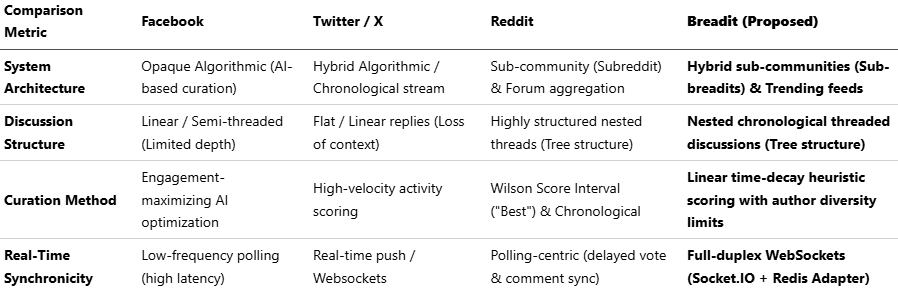
\includegraphics[width=0.92\linewidth,height=0.82\textheight,keepaspectratio]{images/image3.png}
\end{center}


\chapter{METHODOLOGY}

\section{Overview:}

This chapter describes the design methodology, architectural approach, and key technical decisions made during the development of the Breadit hybrid social networking platform. The methodology centers on a systems engineering approach: each architectural decision is evaluated against concrete alternatives based on the platform's defined requirements - real-time content delivery, hybrid feed ranking, threaded discussion management, and community moderation.

The implementation follows a TypeScript-first monorepo strategy using Turborepo, comprising two independently deployable applications: a NestJS/Fastify backend and a Next.js 15 frontend. All major technical choices - architecture pattern, pagination strategy, real-time protocol, and rendering model - are justified by explicit trade-off analysis documented in the sections below.

\section{Development Process:}

\subsection{Architecture Design:}

\begin{longtable}{|p{0.3\linewidth}|p{0.3\linewidth}|p{0.3\linewidth}|}
\caption{Table 16} \label{tab:16} \\
\hline
\textbf{Criterion} & \textbf{Modular Monolith (Chosen)} & \textbf{Microservices} \\
\hline
\endfirsthead
\multicolumn{3}{l}{\textit{(Continued from previous page)}} \\
\hline
\textbf{Criterion} & \textbf{Modular Monolith (Chosen)} & \textbf{Microservices} \\
\hline
\endhead
\hline \multicolumn{3}{r}{\textit{Continued on next page}} \\
\endfoot
\hline
\endlastfoot
Deployment complexity & Single deployable unit per application & Each service requires independent orchestration (Docker Compose, Kubernetes) \\
\hline
Inter-module communication & Direct in-process function calls via NestJS DI & Network calls (REST/gRPC), introducing latency and failure points \\
\hline
Data access & Single shared Prisma client with transactional integrity & Each service manages its own database, requiring distributed transaction patterns (SAGA) \\
\hline
Development overhead & Low - suitable for a single-developer pre-thesis project & High - requires service discovery, API gateways, and distributed logging \\
\hline
Module boundary enforcement & NestJS module encapsulation prevents cross-domain coupling & Enforced by network isolation \\
\hline
Scalability & Horizontal scaling via load balancer; Redis adapter enables stateless instances & Fine-grained per-service scaling \\
\hline
\end{longtable}

\begin{figure}[H]
  \centering
  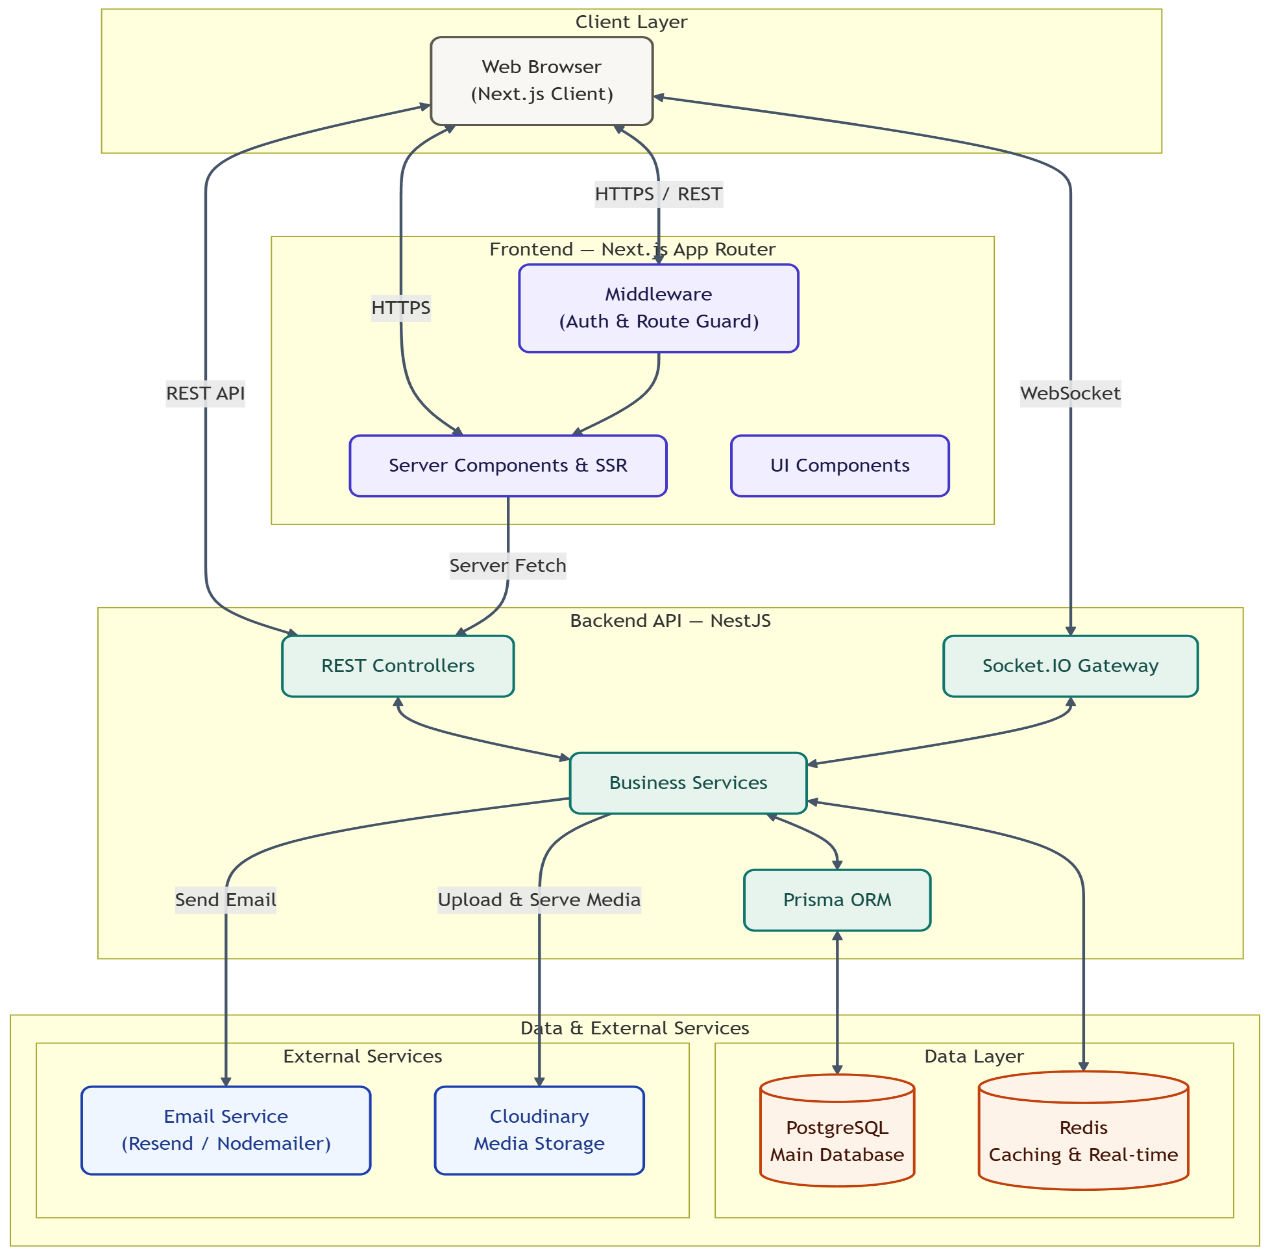
\includegraphics[width=0.92\linewidth,height=0.82\textheight,keepaspectratio]{images/image4.png}
  \caption{High-level architecture diagram}
  \label{fig:1}
\end{figure}

\textbf{Justification}: The Modular Monolithic pattern provides equivalent module isolation to Microservices while eliminating the operational overhead of distributed service orchestration. The NestJS module system enforces strict dependency injection boundaries, preventing domain coupling without requiring network-level separation. Horizontal scalability is still achievable via load-balanced deployments with the Redis-backed Socket.IO adapter, which maintains stateless WebSocket sessions.

\subsubsection{Summary Use Case:}
\begin{enumerate}
  \item Authentication: Guests and users can create accounts, securely log in, verify their email addresses, and reset their passwords.
  \item Content Discovery: Visitors and users can browse chronological feeds and search for specific users, hashtags, or communities.
  \item Post Management: Users can create new posts with rich media attachments, embed hashtags, and edit or delete their own content.
  \item Post Interaction: Users can actively engage with the platform by liking, commenting, replying to threads, reposting, and saving posts.
  \item Relationship Management: Users can follow or unfollow other profiles to curate their personal feed, and block or unblock users for privacy.
  \item Profile Management: Users can update their personal public profiles, including display name, bio, and avatar, and view their activity history.
  \item Direct Messaging: Users can communicate privately with other members through real-time direct messages.
  \item Real-time Notifications: Users receive instant system alerts for social interactions such as new followers, likes, comments, and messages.
  \item Community Management: Users can create specialized communities, join or leave existing groups, and manage community rules and members.
  \item Administrative Moderation: System administrators hold elevated privileges to manage user accounts, apply global bans, and resolve content reports.
\end{enumerate}
\begin{figure}[H]
  \centering
  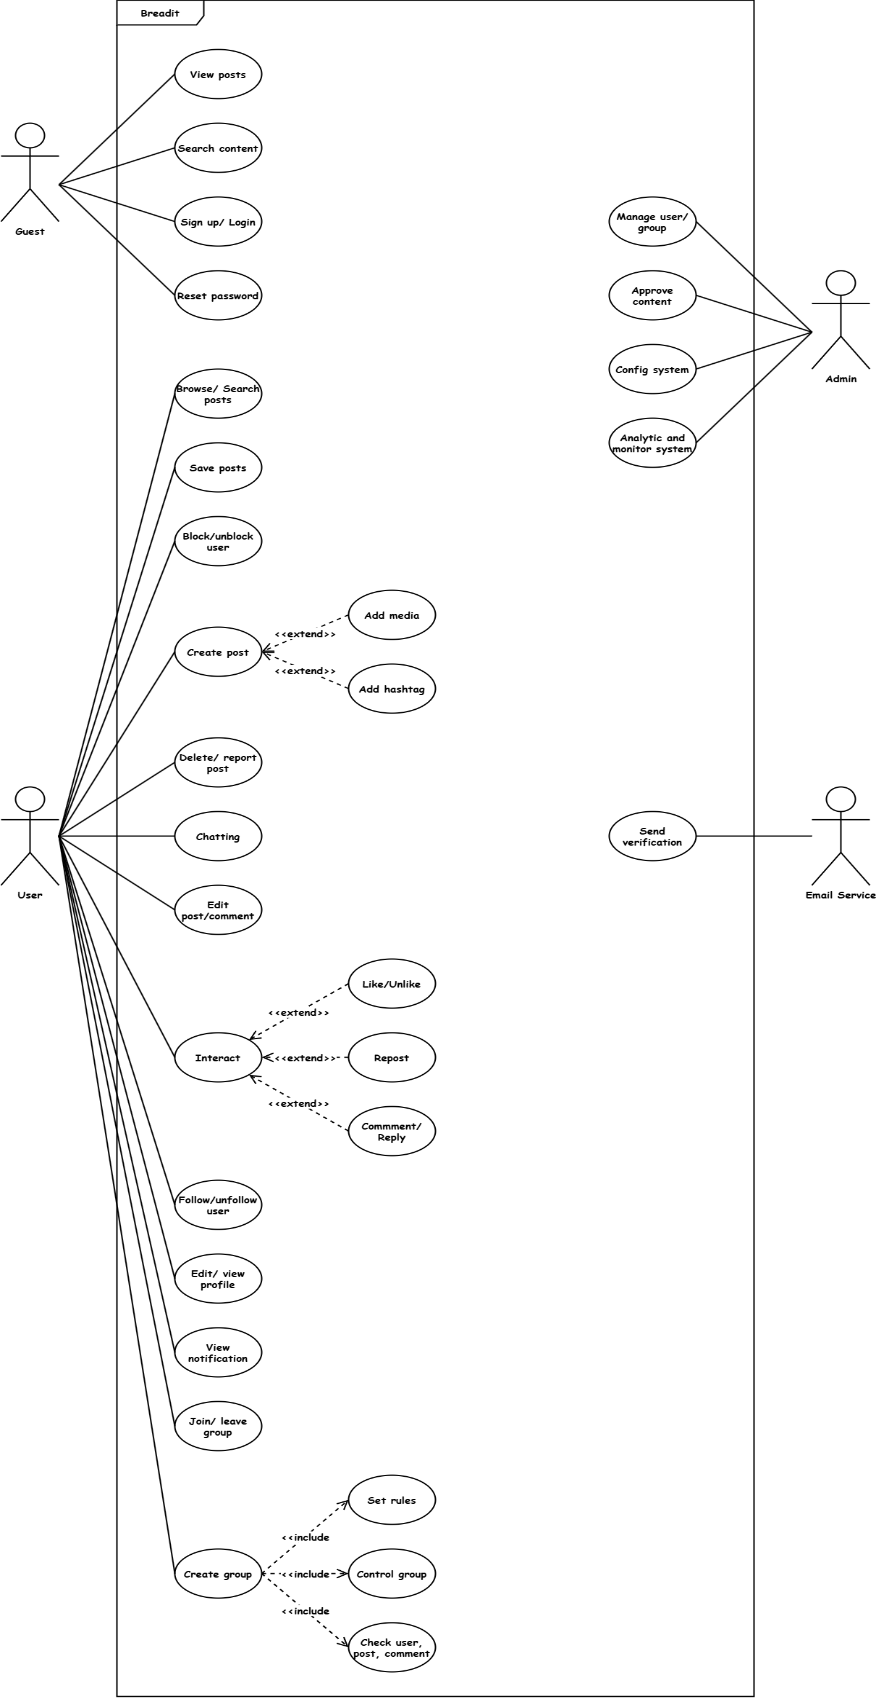
\includegraphics[width=0.92\linewidth,height=0.82\textheight,keepaspectratio]{images/image5.png}
  \caption{Summary Goal Use Case}
  \label{fig:2}
\end{figure}

Actors:
\begin{enumerate}
  \item \textbf{Guest / Unregistered User:}~Can browse public feeds, view user profiles.
  \item \textbf{User / Registered User:}~Can publish micro-blogs, actively interact with content, manage personal connections, send direct messages, and participate in communities.
  \item \textbf{System Admin:}~Manages the platform's integrity by reviewing user-reported content, resolving community disputes, and applying global bans accounts.
\end{enumerate}

\subsubsection{Use Cases:}
\begin{enumerate}
  \item Sign Up/ Login\textbf{:}~Visitors can register a new account to become users.
  \item Verify Email: Users must submit a secure code to verify emails.
  \item Password Recovery: Users can securely reset forgotten passwords via email links.
  \item Manage Profile: Users can update their public bio, avatar, and display name.
  \item View Public Feed: Visitors browse public posts and profiles without authenticating.
  \item Search \& Discovery: Users can search for profiles, communities, trending hashtags.
  \item Create Post: Users can publish micro-blogs and seamlessly attach rich media.
  \item Edit \& Delete Post: Users can modify or permanently remove their published content.
  \item Post Interaction: Users can engage by liking, reposting, or bookmarking posts.
  \item Threaded Comments: Users can participate in multi-level discussion threads posts.
  \item Relationship Management: Users can follow or unfollow accounts to curate feeds.
  \item User Blocking: Users can bidirectionally block accounts to ensure personal privacy.
  \item Direct Messaging: Users communicate privately through a real-time chat interface.
  \item Real-time Notifications: Users receive instant alerts for followers, likes, messages.
  \item Community Management: Users can create specialized communities, manage group
  \item Create Community: Users establish specialized groups for specific topic discussions.
  \item Join/Leave Community: Users can subscribe, unsubscribe from community forums.
  \item Manage Users: System administrators can view user lists and apply bans.
  \item Handle Reports: Administrators can review and resolve content reported by users.
  \item Moderate Content: Administrators can delete inappropriate posts platform guidelines.
\end{enumerate}

\subsubsection{Activity Diagram:}

\medskip\noindent\textbf{Authentication \& Account Management:}\\[2pt]
\begin{figure}[H]
  \centering
  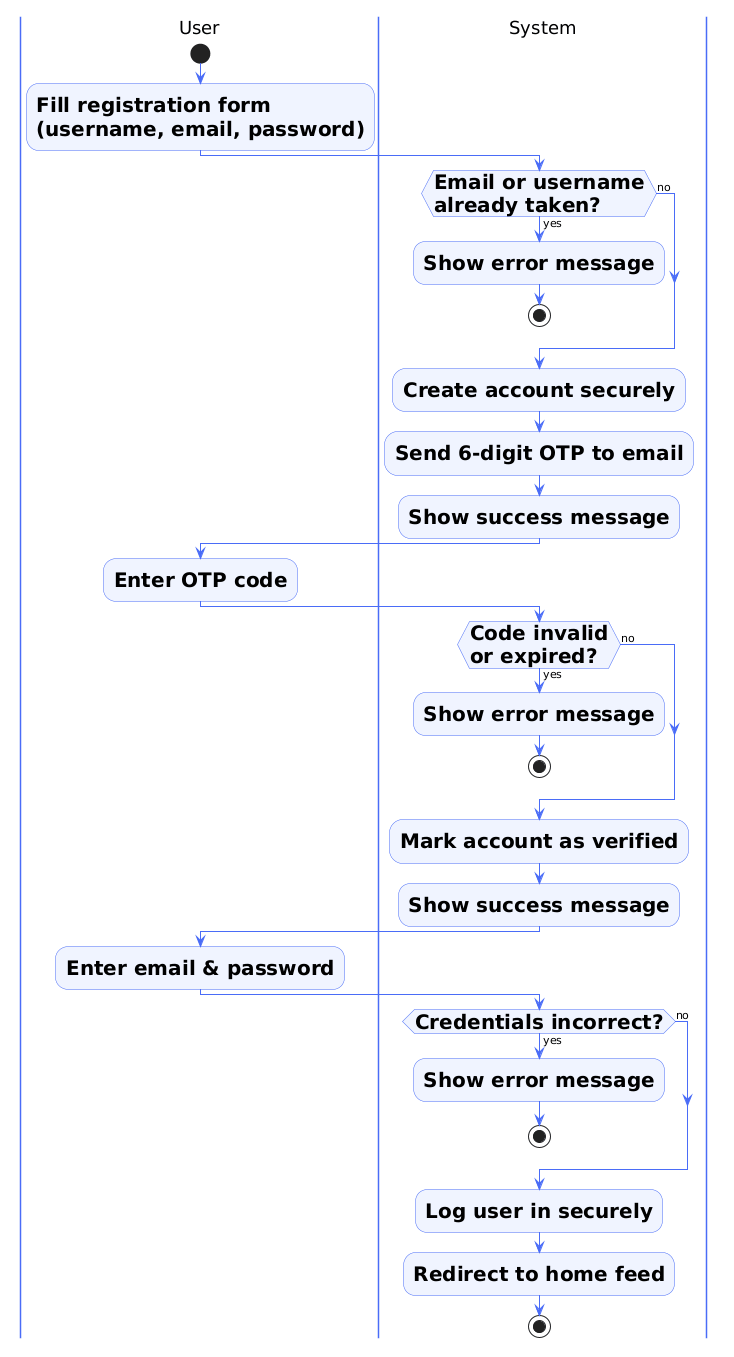
\includegraphics[width=0.92\linewidth,height=0.82\textheight,keepaspectratio]{images/image6.png}
  \caption{Authentication \& Account Management}
  \label{fig:3}
\end{figure}

\medskip\noindent\textbf{Feeds and Discovery:}\\[2pt]
\begin{figure}[H]
  \centering
  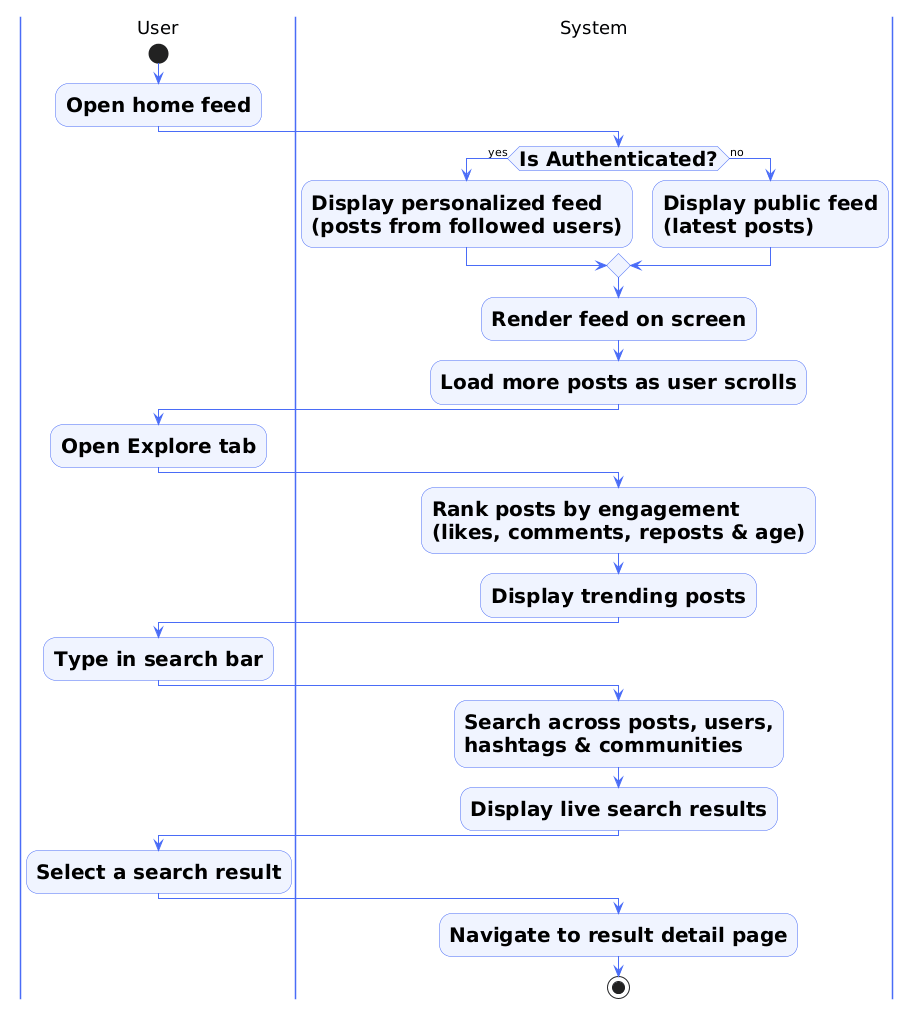
\includegraphics[width=0.92\linewidth,height=0.82\textheight,keepaspectratio]{images/image7.png}
  \caption{Feeds and Discovery}
  \label{fig:4}
\end{figure}

\medskip\noindent\textbf{Post Management:}\\[2pt]
\begin{figure}[H]
  \centering
  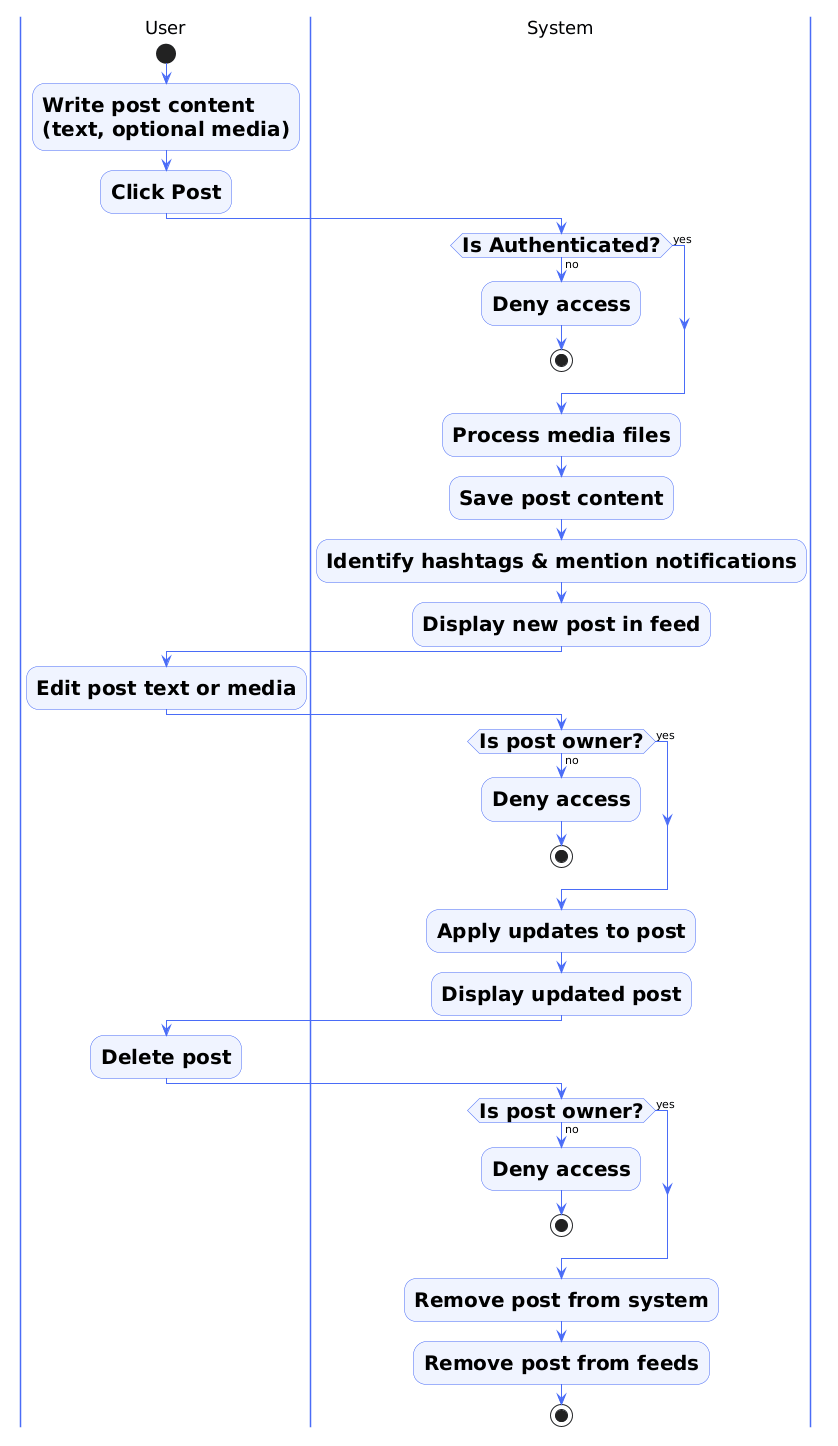
\includegraphics[width=0.92\linewidth,height=0.82\textheight,keepaspectratio]{images/image8.png}
  \caption{Post Management}
  \label{fig:5}
\end{figure}

\medskip\noindent\textbf{Post Interaction:}\\[2pt]
\begin{figure}[H]
  \centering
  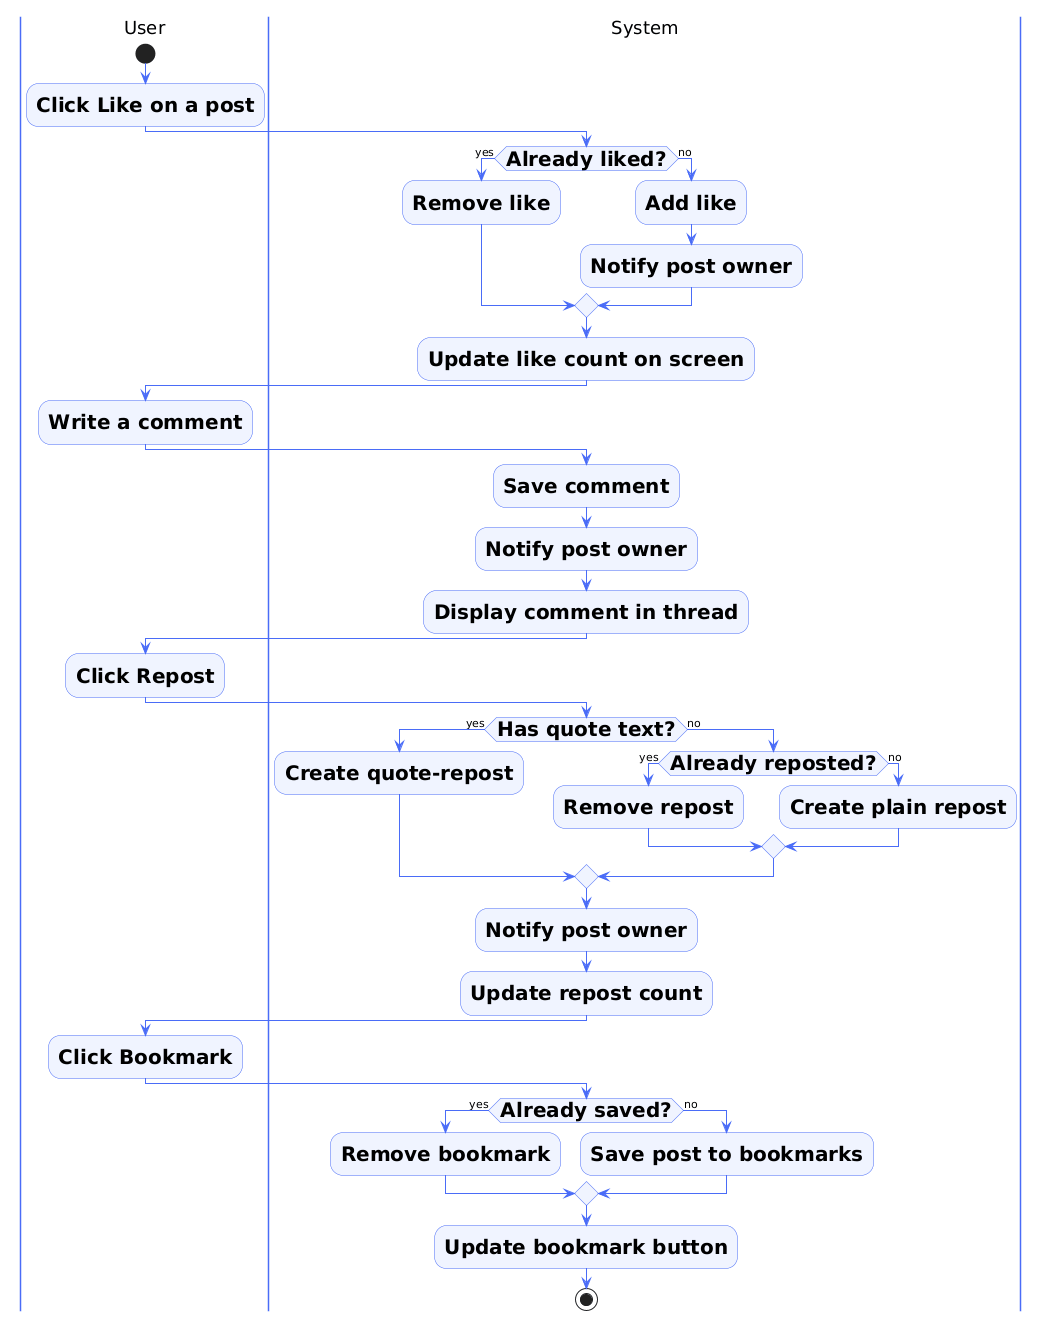
\includegraphics[width=0.92\linewidth,height=0.82\textheight,keepaspectratio]{images/image9.png}
  \caption{Post Interaction}
  \label{fig:6}
\end{figure}

\medskip\noindent\textbf{User Relationship Management:}\\[2pt]
\begin{figure}[H]
  \centering
  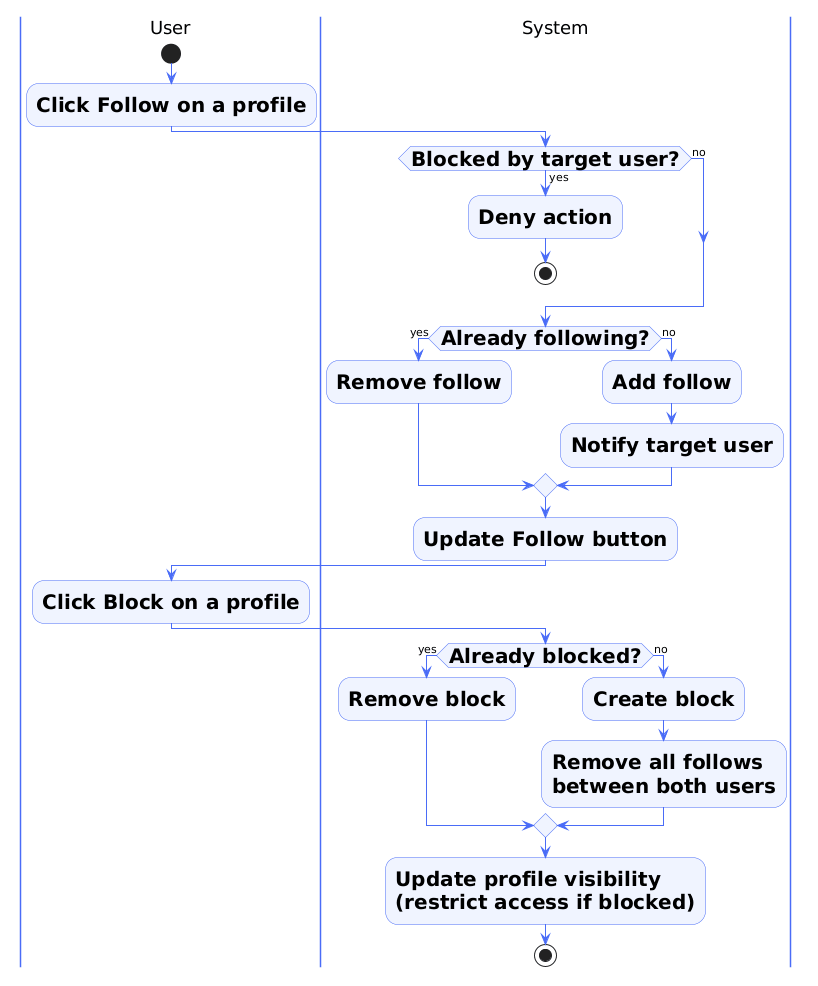
\includegraphics[width=0.92\linewidth,height=0.82\textheight,keepaspectratio]{images/image10.png}
  \caption{User Relationship Management}
  \label{fig:7}
\end{figure}

\medskip\noindent\textbf{User Profile Management:}\\[2pt]
\begin{figure}[H]
  \centering
  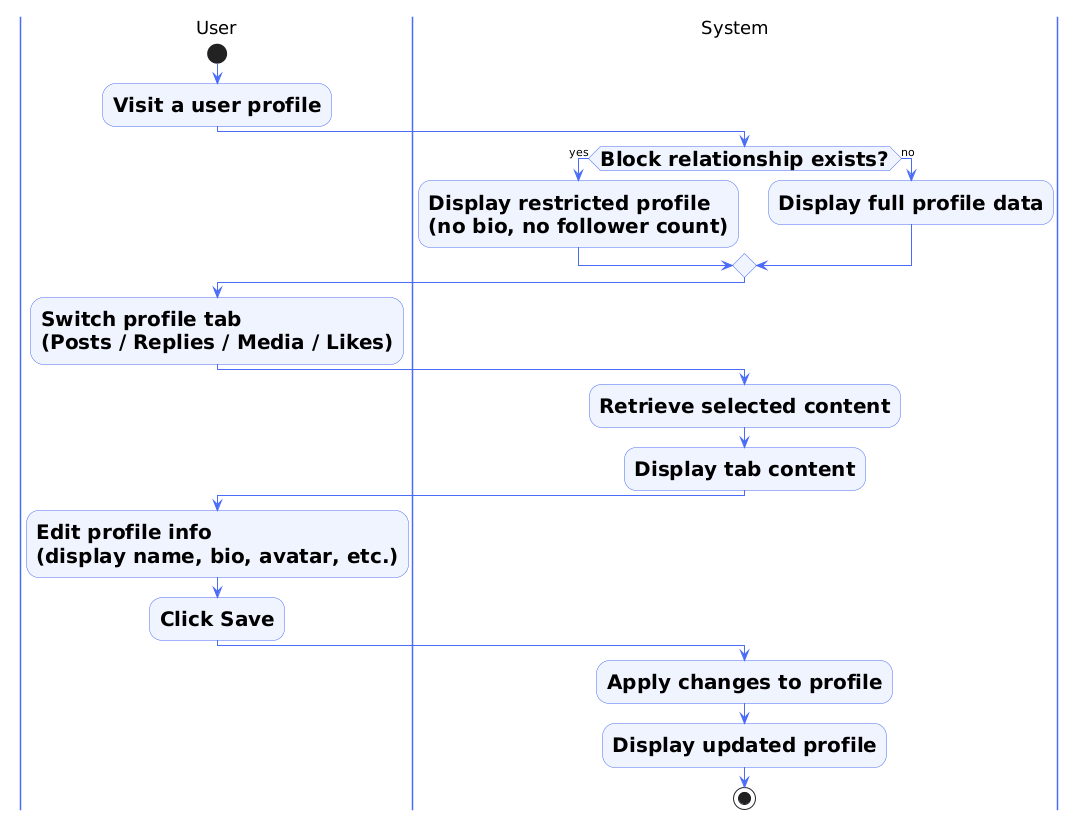
\includegraphics[width=0.92\linewidth,height=0.82\textheight,keepaspectratio]{images/image11.png}
  \caption{User Profile Management}
  \label{fig:8}
\end{figure}

\medskip\noindent\textbf{Direct Messaging:}\\[2pt]
\begin{figure}[H]
  \centering
  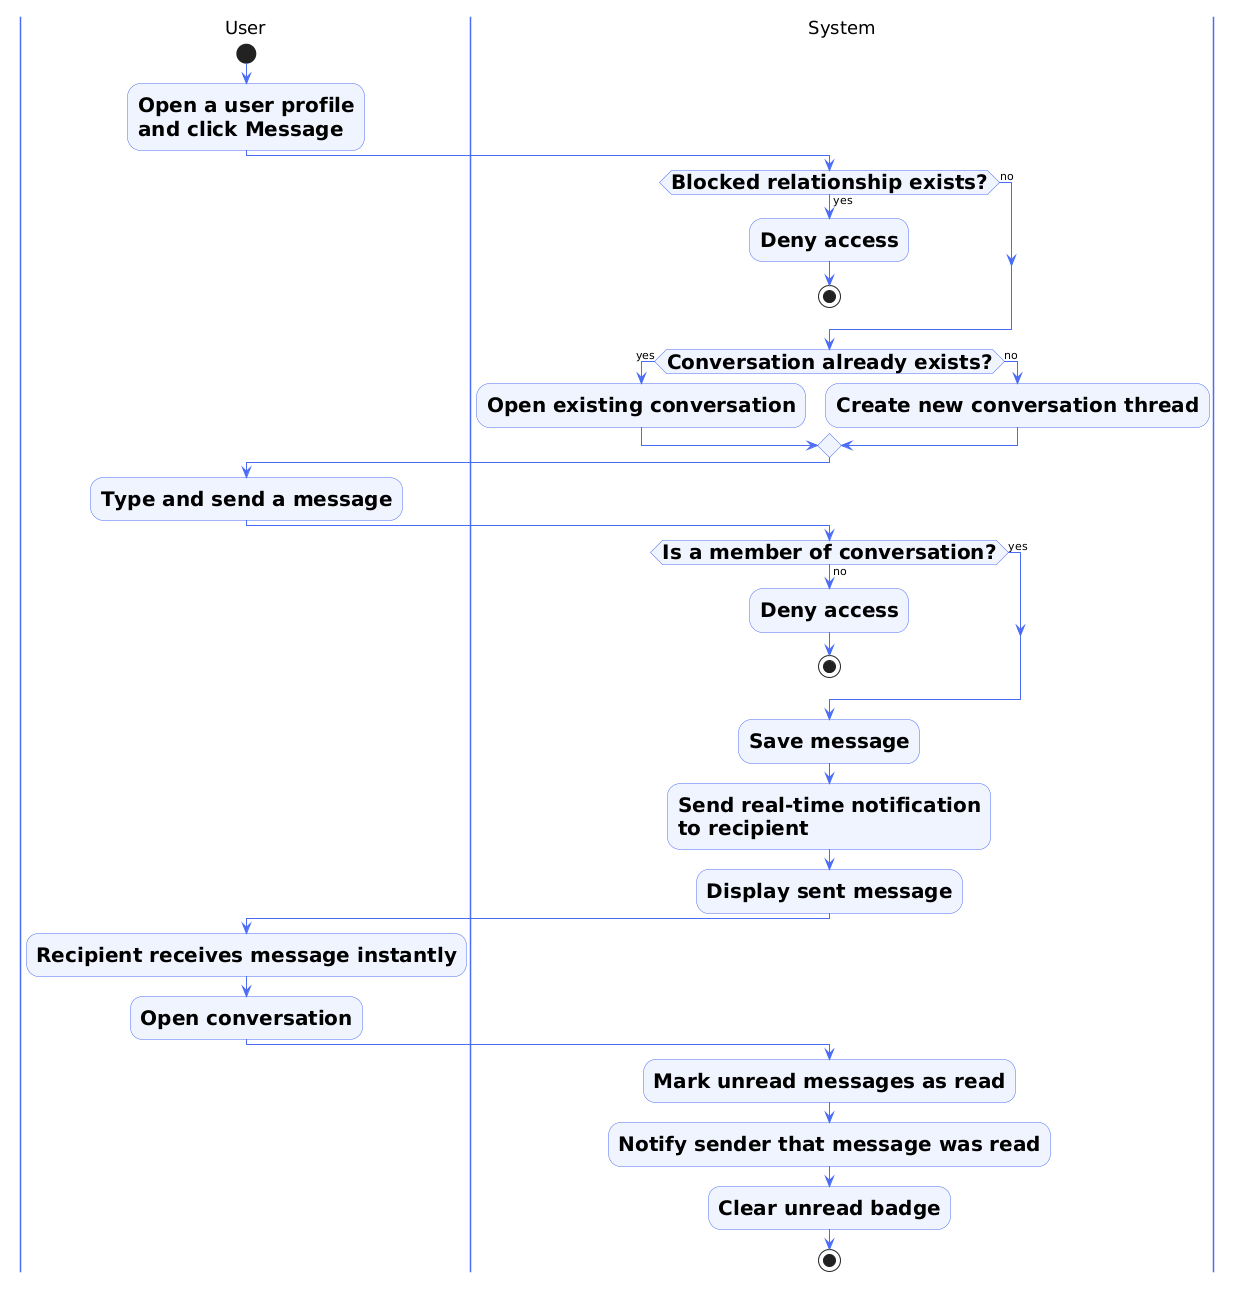
\includegraphics[width=0.92\linewidth,height=0.82\textheight,keepaspectratio]{images/image12.png}
  \caption{Direct Messaging}
  \label{fig:9}
\end{figure}

\medskip\noindent\textbf{Real-time Notifications:}\\[2pt]
\begin{figure}[H]
  \centering
  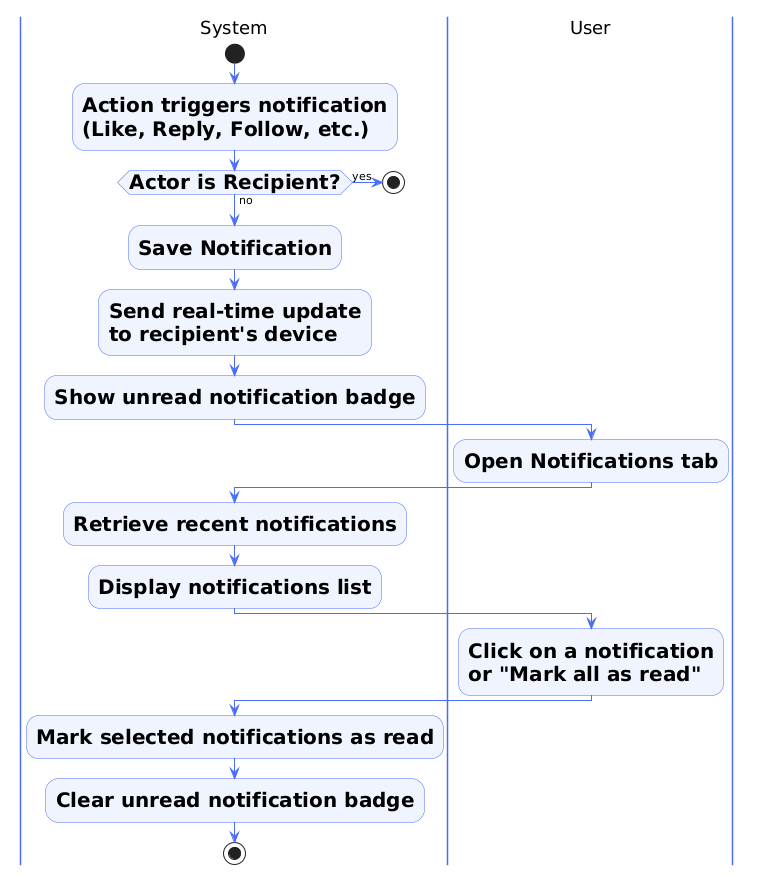
\includegraphics[width=0.92\linewidth,height=0.82\textheight,keepaspectratio]{images/image13.png}
  \caption{Real-time Notifications}
  \label{fig:10}
\end{figure}

\medskip\noindent\textbf{Community Management:}\\[2pt]
\begin{figure}[H]
  \centering
  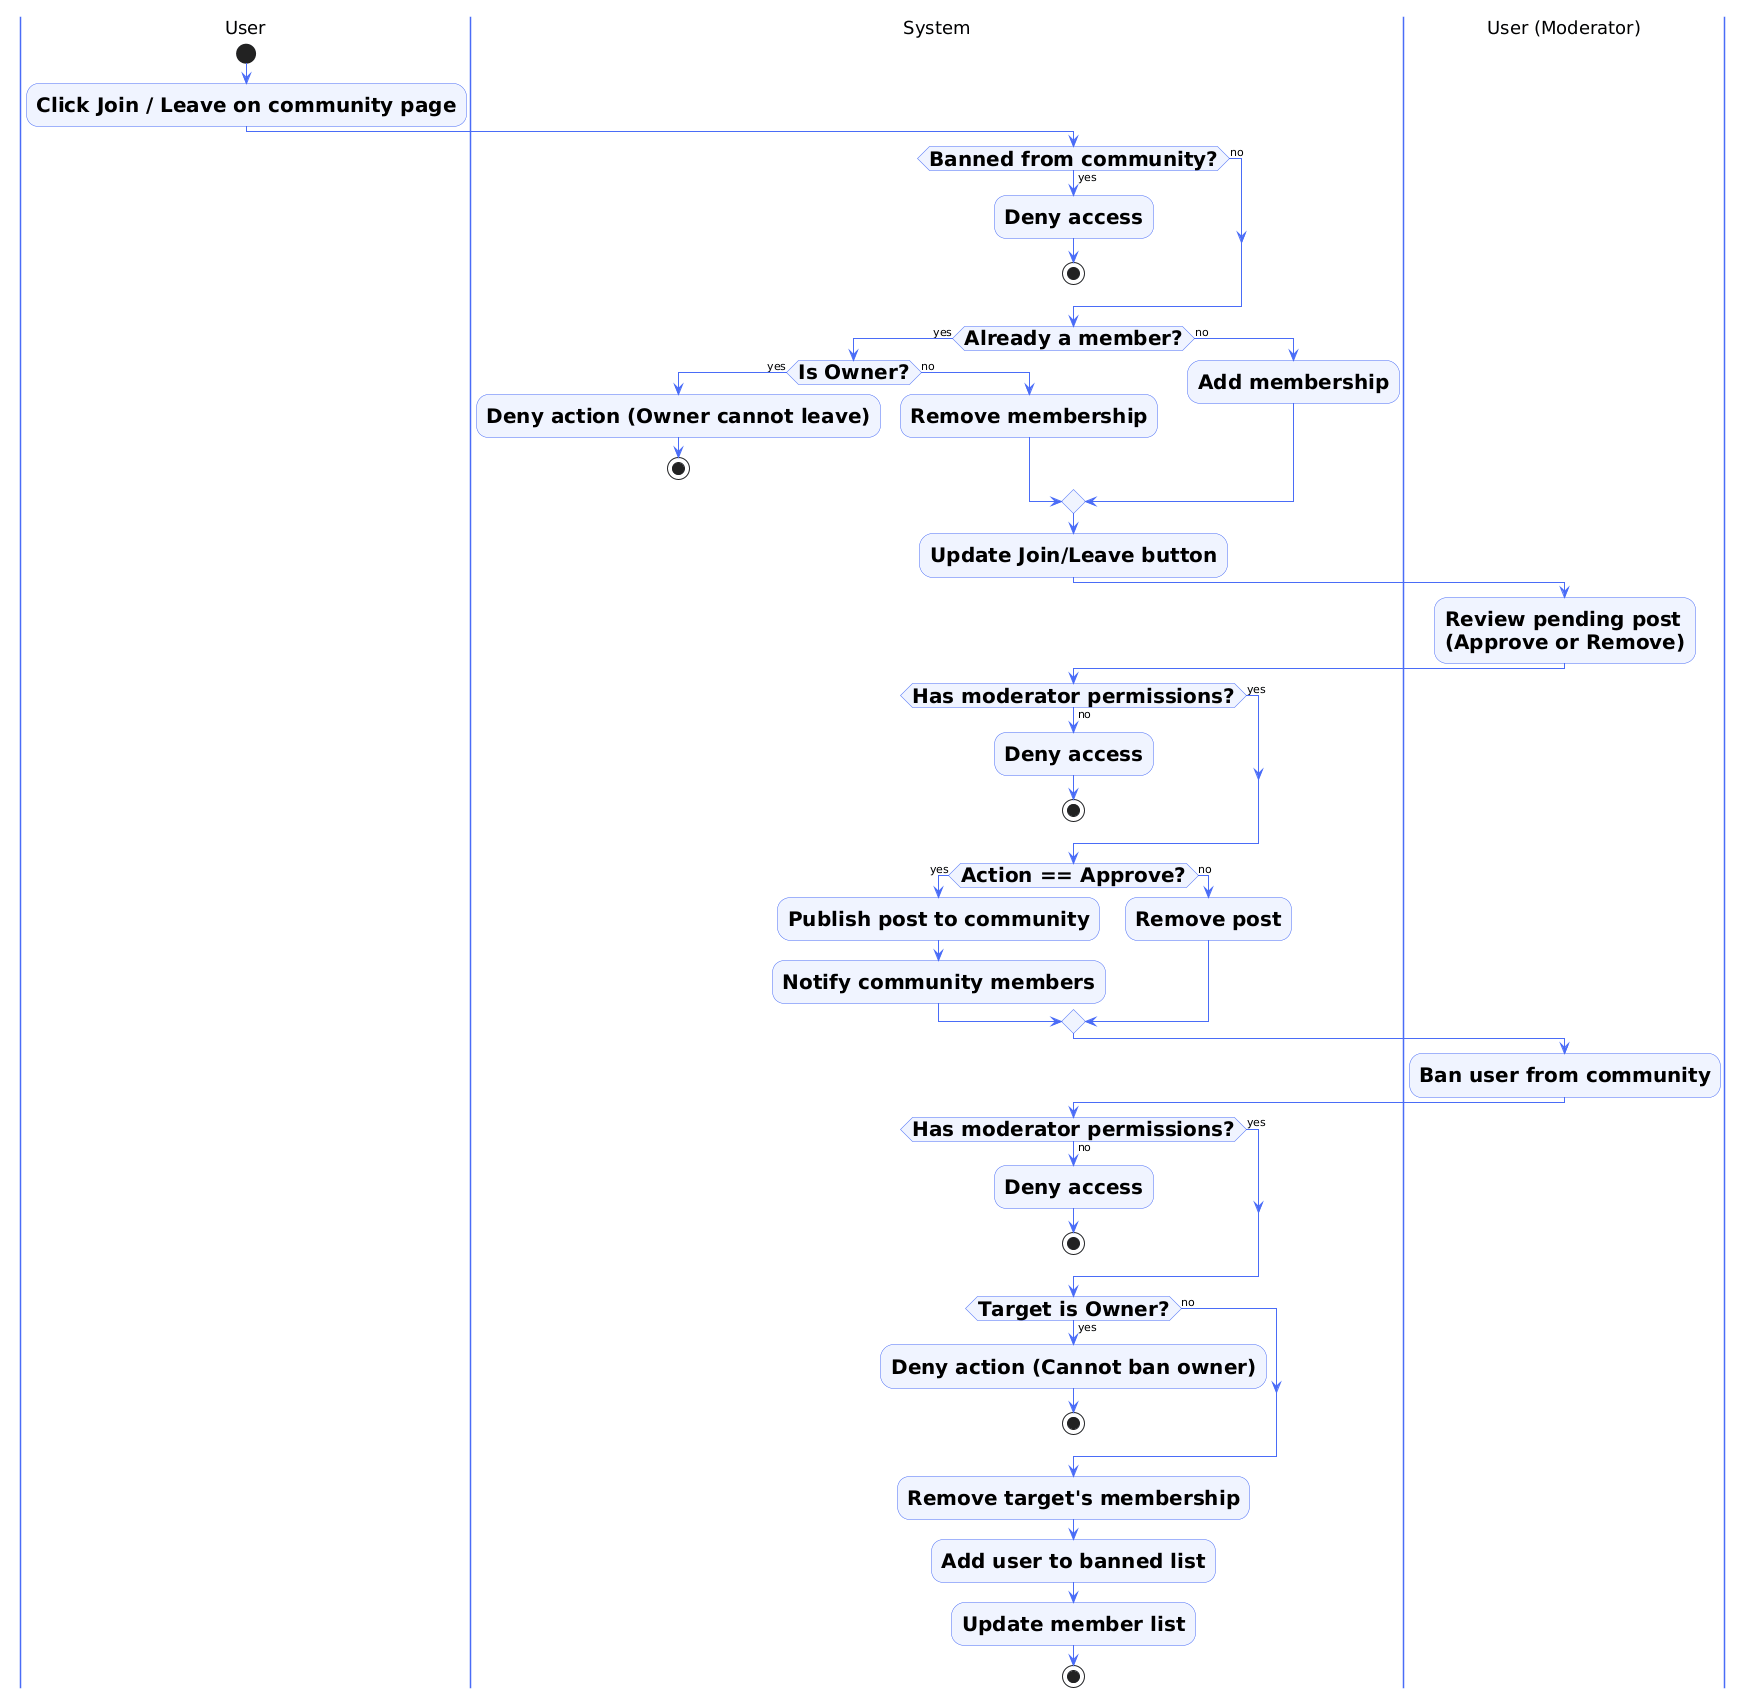
\includegraphics[width=0.92\linewidth,height=0.82\textheight,keepaspectratio]{images/image14.png}
  \caption{Community Management}
  \label{fig:11}
\end{figure}

\medskip\noindent\textbf{Administrative Moderation:}\\[2pt]
\begin{figure}[H]
  \centering
  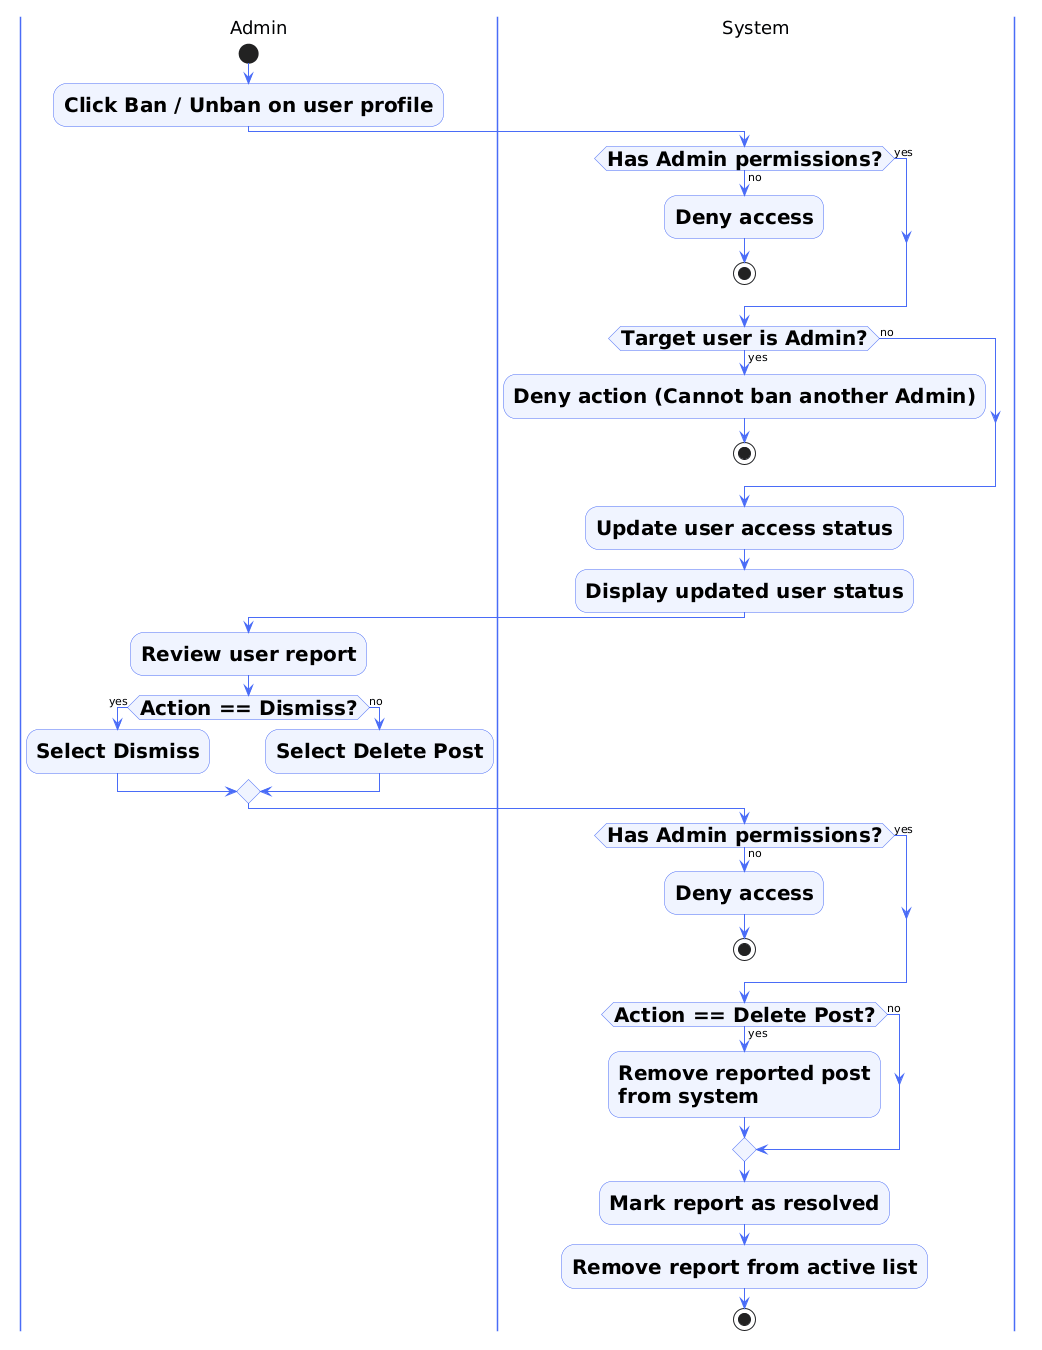
\includegraphics[width=0.92\linewidth,height=0.82\textheight,keepaspectratio]{images/image15.png}
  \caption{Administrative Moderation}
  \label{fig:12}
\end{figure}

\subsubsection{Entity Relationship Diagram:}
\begin{figure}[H]
  \centering
  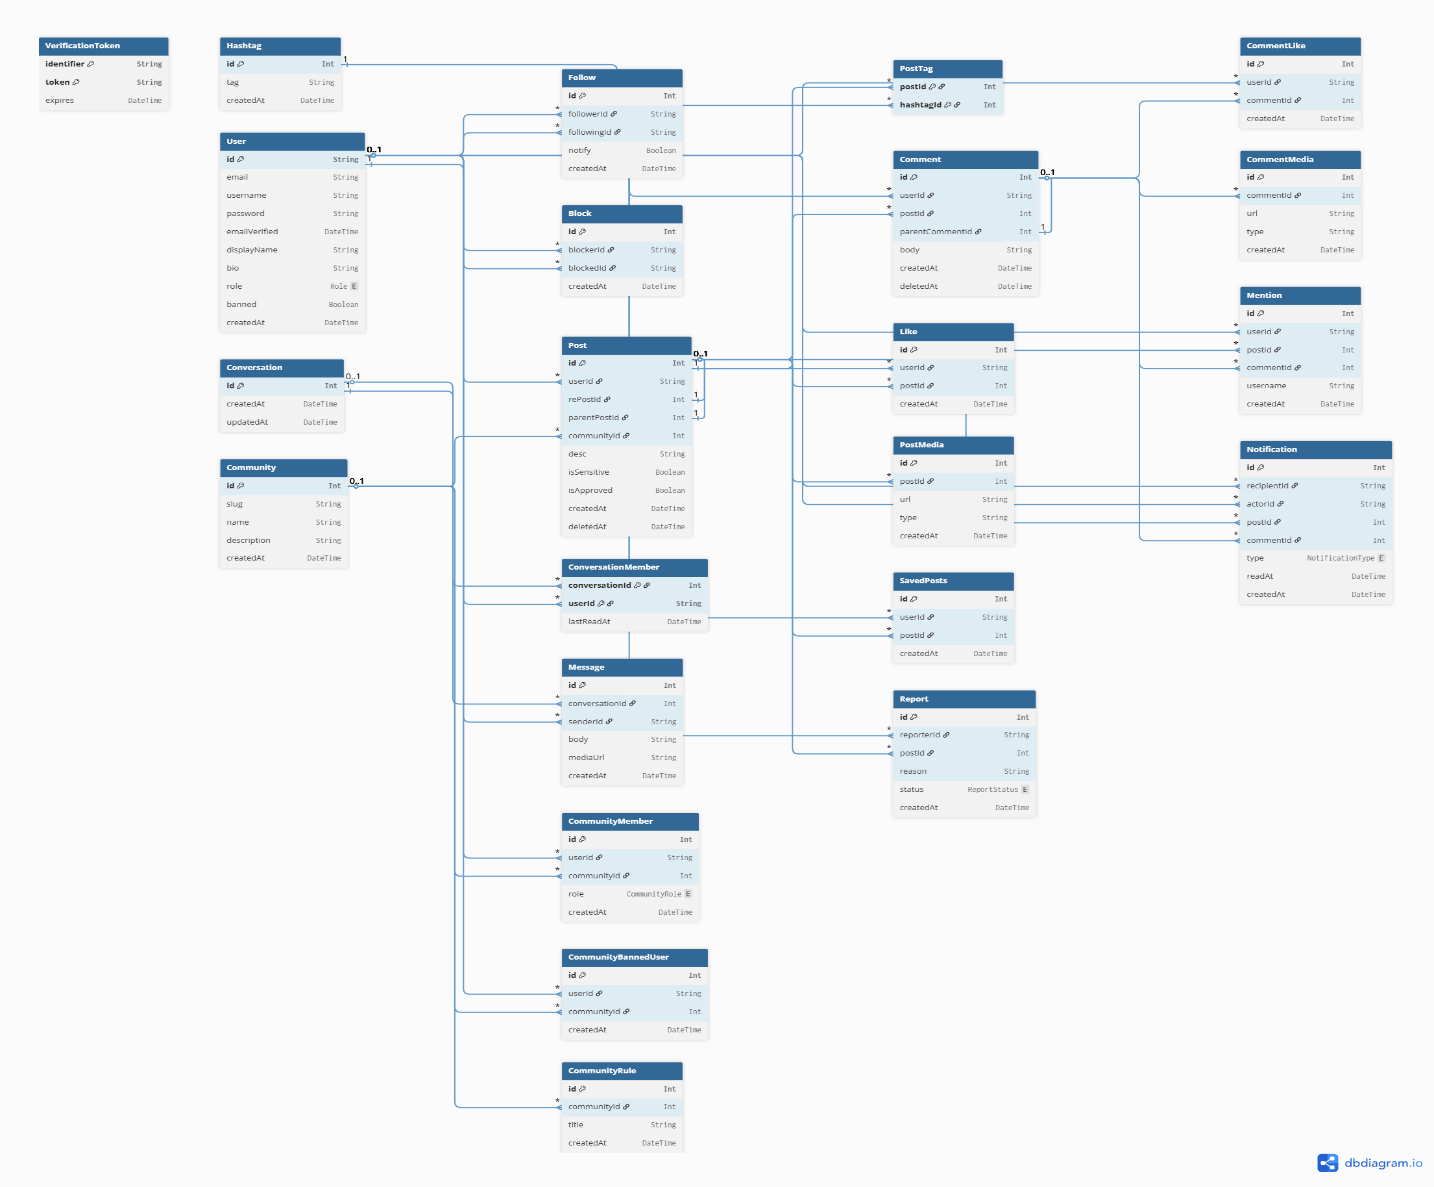
\includegraphics[width=0.92\linewidth,height=0.82\textheight,keepaspectratio]{images/image17.png}
  \caption{Entity Relationship Diagram}
  \label{fig:13}
\end{figure}

This section covers the all-database entities (tables) for the project. A more detailed and higher resolution version of the Entity Relationship Diagram is available in the Appendix section.

Summary:
\begin{enumerate}
  \item \textbf{Identity \& Access }\textbf{-Related Tables}
\end{enumerate}
\begin{figure}[H]
  \centering
  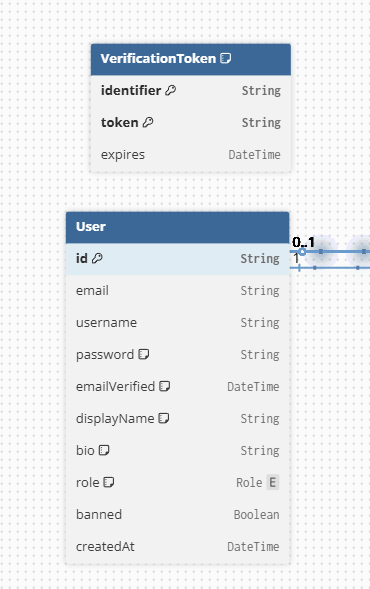
\includegraphics[width=0.92\linewidth,height=0.82\textheight,keepaspectratio]{images/image18.png}
  \caption{Identity \& Access -- Related Tables}
  \label{fig:14}
\end{figure}

\begin{longtable}{|p{0.45\linewidth}|p{0.45\linewidth}|}
\caption{Identity \& Access - Related Tables} \label{tab:17} \\
\hline
\textbf{\textbullet User  Description:~Core entity representing every platform account, storing identity, profile, and system-level access state.  Fields:}\newline id~(PK, String, cuid)\newline email~(String, unique)\newline username~(String, unique)\newline password~(String, nullable)\newline emailVerified~(DateTime, nullable)\newline displayName~(String, nullable)\newline bio~(String, nullable)\newline location~(String, nullable)\newline job~(String, nullable)\newline website~(String, nullable)\newline img~(String, nullable)\newline cover~(String, nullable)\newline role~(Enum: USER | ADMIN)\newline banned~(Boolean, default: false)\newline createdAt~/~updatedAt~(DateTime)\newline Relationships:\newline One-to-Many with interaction tables (Post, Comment, Like, etc.) & \textbf{\textbullet VerificationToken  Description:~Stores single-use OTP codes for email verification and password reset flows. Automatically deleted after use or expiry.  Fields:}\newline identifier~(PK, String) - e.g., "email-verify:user123"\newline token~(PK, String) - 6-digit OTP or UUID string\newline expires~(DateTime) - Expiration timestamp\newline Relationships:\newline One-to-Many with nearly all other tables (Post, Comment, Like, Follow, etc. \\
\hline
\endfirsthead
\multicolumn{2}{l}{\textit{(Continued from previous page)}} \\
\hline
\textbf{\textbullet User  Description:~Core entity representing every platform account, storing identity, profile, and system-level access state.  Fields:}\newline id~(PK, String, cuid)\newline email~(String, unique)\newline username~(String, unique)\newline password~(String, nullable)\newline emailVerified~(DateTime, nullable)\newline displayName~(String, nullable)\newline bio~(String, nullable)\newline location~(String, nullable)\newline job~(String, nullable)\newline website~(String, nullable)\newline img~(String, nullable)\newline cover~(String, nullable)\newline role~(Enum: USER | ADMIN)\newline banned~(Boolean, default: false)\newline createdAt~/~updatedAt~(DateTime)\newline Relationships:\newline One-to-Many with interaction tables (Post, Comment, Like, etc.) & \textbf{\textbullet VerificationToken  Description:~Stores single-use OTP codes for email verification and password reset flows. Automatically deleted after use or expiry.  Fields:}\newline identifier~(PK, String) - e.g., "email-verify:user123"\newline token~(PK, String) - 6-digit OTP or UUID string\newline expires~(DateTime) - Expiration timestamp\newline Relationships:\newline One-to-Many with nearly all other tables (Post, Comment, Like, Follow, etc. \\
\hline
\endhead
\hline \multicolumn{2}{r}{\textit{Continued on next page}} \\
\endfoot
\hline
\endlastfoot
\end{longtable}

\begin{enumerate}
  \item \textbf{Content }\textbf{-Related Table}\textbf{s}
\end{enumerate}
\begin{figure}[H]
  \centering
  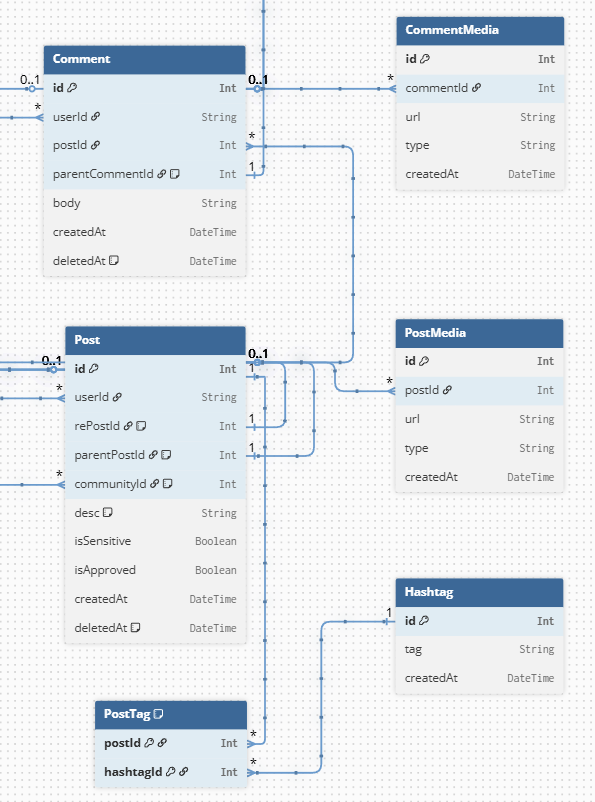
\includegraphics[width=0.92\linewidth,height=0.82\textheight,keepaspectratio]{images/image19.png}
  \caption{Content -- Related Tables}
  \label{fig:15}
\end{figure}

\begin{longtable}{|p{0.45\linewidth}|p{0.45\linewidth}|}
\caption{Content -Related Tables} \label{tab:18} \\
\hline
\textbf{\textbullet Post Description:~The backbone of the feed. Represents original post, repost, and through self-referencing belong community.}\newline Fields:\newline id~(PK, Int)\newline userId~(FK, String) - The author\newline communityId~(FK, Int, nullable)\newline desc~(String, nullable)\newline isSensitive~(Boolean\newline isApproved~(Boolean)\newline rePostId~(FK, Int, nullable)\newline parentPostId~(FK, Int, nullable) -\newline deletedAt~(DateTime, nullable)\newline Relationships:\newline Self-reference for reposts\newline Many-to-One with User, Community\newline One-to-Many with PostMedia, Comment, Like, SavedPosts, PostTag, Notification, Report, Mention & \textbf{\textbullet PostMedia Description:~Stores images/videos attached Post.}\newline Fields:\newline id (PK, Int)\newline postId (FK, Int)\newline url (String) CDN path (Cloudinary/S3)\newline type (String) --- "IMAGE" | "VIDEO" | "FILE"\newline width, height (Int, nullable) Used for layout rendering\newline createdAt (DateTime)\newline Relationships:\newline Many-to-One with~Post~(Cascade delete) \\
\hline
\endfirsthead
\multicolumn{2}{l}{\textit{(Continued from previous page)}} \\
\hline
\textbf{\textbullet Post Description:~The backbone of the feed. Represents original post, repost, and through self-referencing belong community.}\newline Fields:\newline id~(PK, Int)\newline userId~(FK, String) - The author\newline communityId~(FK, Int, nullable)\newline desc~(String, nullable)\newline isSensitive~(Boolean\newline isApproved~(Boolean)\newline rePostId~(FK, Int, nullable)\newline parentPostId~(FK, Int, nullable) -\newline deletedAt~(DateTime, nullable)\newline Relationships:\newline Self-reference for reposts\newline Many-to-One with User, Community\newline One-to-Many with PostMedia, Comment, Like, SavedPosts, PostTag, Notification, Report, Mention & \textbf{\textbullet PostMedia Description:~Stores images/videos attached Post.}\newline Fields:\newline id (PK, Int)\newline postId (FK, Int)\newline url (String) CDN path (Cloudinary/S3)\newline type (String) --- "IMAGE" | "VIDEO" | "FILE"\newline width, height (Int, nullable) Used for layout rendering\newline createdAt (DateTime)\newline Relationships:\newline Many-to-One with~Post~(Cascade delete) \\
\hline
\endhead
\hline \multicolumn{2}{r}{\textit{Continued on next page}} \\
\endfoot
\hline
\endlastfoot
\textbullet Comment Description:~Stores user replies to a Post. Fields:\newline id (PK, Int)\newline postId (FK, Int)\newline url (String) CDN path (Cloudinary/S3)\newline type (String) --- "IMAGE" | "VIDEO" | "FILE"\newline width, height (Int, nullable)\newline createdAt (DateTime)\newline Relationships:\newline Self-referencing nested comment tree\newline Many-to-One with User, Post\newline One-to-Many with CommentMedia, CommentLike, Mention, Notification & \textbullet CommentMedia Description:~File attachments inside comments. Fields:\newline id (PK, Int)\newline commentId (FK, Int)\newline url (String) CDN path\newline type (String) --- "IMAGE" | "VIDEO" | "FILE"\newline width, height (Int, nullable)\newline createdAt (DateTime)\newline Relationships:\newline Many-to-One with~Comment \\
\hline
\textbullet Hashtag Description:~Normalized registry of tags to serve the Trending feature. Fields:\newline id (PK, Int)\newline tag (String, unique) Lowercase tag string, e.g. "technology"\newline createdAt (DateTime)\newline Relationships:\newline One-to-Many with~PostTag & \textbullet PostTag Description:~Join table resolving the Many-to-Many relationship between Posts and Hashtags. Created/updated automatically when a post is submitted or edited. Fields:\newline postId~(PK, FK, Int)\newline hashtagId~(PK, FK, Int)\newline Relationships:\newline Composite Primary Key with 2 FKs. \\
\hline
\end{longtable}

\begin{enumerate}
  \item \textbf{Social Engagement}\textbf{ Tables}
\end{enumerate}
\begin{figure}[H]
  \centering
  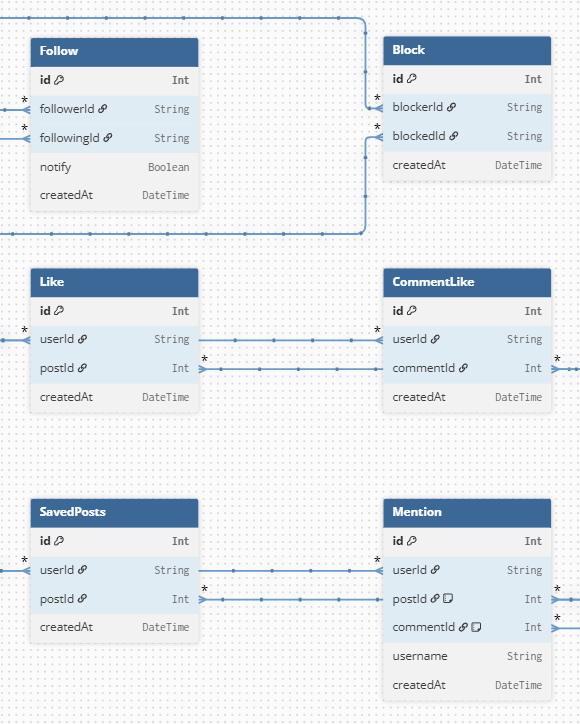
\includegraphics[width=0.92\linewidth,height=0.82\textheight,keepaspectratio]{images/image20.png}
  \caption{Social Engagement -- Related Tables}
  \label{fig:16}
\end{figure}

\begin{longtable}{|p{0.45\linewidth}|p{0.45\linewidth}|}
\caption{Social Engagement -- Related Tables} \label{tab:19} \\
\hline
\textbf{\textbullet  Follow Description:~Directed social graph edge. Determines which users appear in the personalized home feed of the follower. Fields:}\newline id (PK, Int)\newline followerId (FK, String)\newline followingId (FK, String)\newline notify (Boolean, default: false) Push notification preference for this specific follow\newline createdAt (DateTime)\newline Relationships:\newline Many-to-One with User twice (follower and following sides) & \textbf{\textbullet Block  Description:~Mutual blacklist between two users. Prevents all interactions (follow, message, view posts). Automatically removes existing follows between both parties. Fields:}\newline id (PK, Int)\newline blockerId (FK, String) --- The user initiating the block\newline blockedId (FK, String) --- The user being blocked\newline createdAt (DateTime)\newline Relationships:\newline Many-to-One with User twice.\newline Unique constraint on [blockerId, blockedId]. \\
\hline
\endfirsthead
\multicolumn{2}{l}{\textit{(Continued from previous page)}} \\
\hline
\textbf{\textbullet  Follow Description:~Directed social graph edge. Determines which users appear in the personalized home feed of the follower. Fields:}\newline id (PK, Int)\newline followerId (FK, String)\newline followingId (FK, String)\newline notify (Boolean, default: false) Push notification preference for this specific follow\newline createdAt (DateTime)\newline Relationships:\newline Many-to-One with User twice (follower and following sides) & \textbf{\textbullet Block  Description:~Mutual blacklist between two users. Prevents all interactions (follow, message, view posts). Automatically removes existing follows between both parties. Fields:}\newline id (PK, Int)\newline blockerId (FK, String) --- The user initiating the block\newline blockedId (FK, String) --- The user being blocked\newline createdAt (DateTime)\newline Relationships:\newline Many-to-One with User twice.\newline Unique constraint on [blockerId, blockedId]. \\
\hline
\endhead
\hline \multicolumn{2}{r}{\textit{Continued on next page}} \\
\endfoot
\hline
\endlastfoot
\textbullet   Like Description:~Records a User's "like" reaction on a Post. Triggers a LIKE notification to the post author. Fields:\newline id (PK, Int)\newline userId (FK, String)\newline postId (FK, Int)\newline createdAt (DateTime)\newline Relationships:\newline Many-to-One with User, Post & \textbullet  CommentLike\newline Description: Records a User's "like" reaction on a Comment. Unique constraint prevents double-liking.\newline Fields:\newline id (PK, Int)\newline userId (FK, String)\newline commentId (FK, Int)\newline createdAt (DateTime)\newline Relationships:\newline Many-to-One with User, Comment (Cascade delete)\newline Unique constraint on [userId, commentId] \\
\hline
\textbullet  SavedPosts\newline Description: User's personal bookmark list. Posts saved here appear in the /bookmarks.\newline Fields:\newline id (PK, Int)\newline userId (FK, String)\newline postId (FK, Int)\newline createdAt (DateTime)\newline Relationships:\newline Many-to-One with User, Post & \textbullet  Mention\newline Description: Records every @username tag inside a post or comment body. Parsed automatically on create/edit. Triggers a MENTION notification to the tagged user.\newline Fields:\newline id (PK, Int)\newline userId (FK, String)\newline username (String)\newline postId (FK, Int, nullable)\newline commentId (FK, Int, nullable)\newline createdAt (DateTime)\newline Relationships:\newline Many-to-One with User, Post, Comment (Cascade delete) \\
\hline
\end{longtable}

\begin{enumerate}
  \item \textbf{Community \& Moderation}\textbf{ Tables}
\end{enumerate}
\begin{figure}[H]
  \centering
  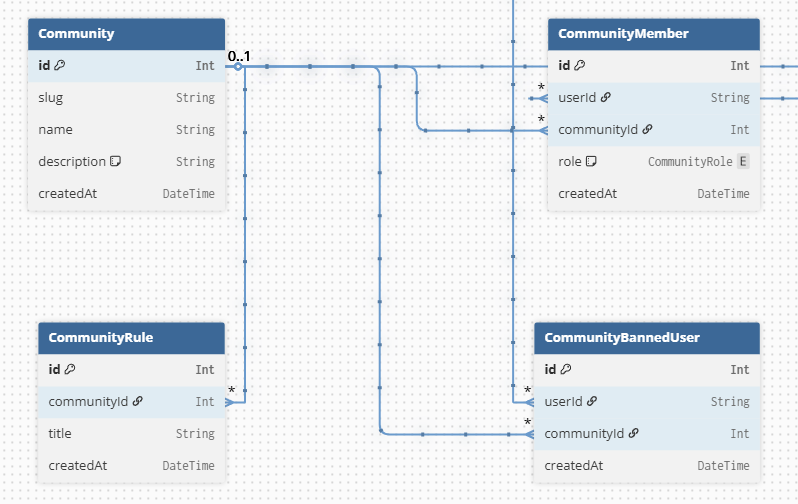
\includegraphics[width=0.92\linewidth,height=0.82\textheight,keepaspectratio]{images/image21.png}
  \caption{Community \& Moderation - Related Tables}
  \label{fig:17}
\end{figure}

\begin{longtable}{|p{0.45\linewidth}|p{0.45\linewidth}|}
\caption{Community \& Moderation Tables} \label{tab:20} \\
\hline
\textbf{\textbullet       Community Description:~Represents a Sub-reddit style group, a shared space for members with common interests. Fields:}\newline id (PK, Int)\newline slug (String, unique) URL identifier, e.g. breadit.com/c/technology\newline name (String) Display name\newline description (String, nullable)\newline img (String, nullable)\newline cover (String, nullable)\newline createdAt / updatedAt (DateTime)\newline Relationships:\newline One-to-Many with Post, Member, Rule, BannedUser & \textbf{CommunityMember Description:~Unique Constraint: 1 User can join a specific community only once.}\newline Fields:\newline id (PK, Int)\newline userId (FK, String)\newline communityId (FK, Int)\newline role (Enum: MEMBER | MOD | OWNER, default: MEMBER)\newline createdAt (DateTime)\newline Relationships:\newline Many-to-One with User, Community\newline Unique constraint on [userId, communityId] one role per user per community \\
\hline
\endfirsthead
\multicolumn{2}{l}{\textit{(Continued from previous page)}} \\
\hline
\textbf{\textbullet       Community Description:~Represents a Sub-reddit style group, a shared space for members with common interests. Fields:}\newline id (PK, Int)\newline slug (String, unique) URL identifier, e.g. breadit.com/c/technology\newline name (String) Display name\newline description (String, nullable)\newline img (String, nullable)\newline cover (String, nullable)\newline createdAt / updatedAt (DateTime)\newline Relationships:\newline One-to-Many with Post, Member, Rule, BannedUser & \textbf{CommunityMember Description:~Unique Constraint: 1 User can join a specific community only once.}\newline Fields:\newline id (PK, Int)\newline userId (FK, String)\newline communityId (FK, Int)\newline role (Enum: MEMBER | MOD | OWNER, default: MEMBER)\newline createdAt (DateTime)\newline Relationships:\newline Many-to-One with User, Community\newline Unique constraint on [userId, communityId] one role per user per community \\
\hline
\endhead
\hline \multicolumn{2}{r}{\textit{Continued on next page}} \\
\endfoot
\hline
\endlastfoot
\textbullet         CommunityRule Description:~Custom rules and regulations set by Community Admins. Fields:\newline id (PK, Int)\newline communityId (FK, Int)\newline title (String) - Rule headline\newline Relationships:\newline Many-to-One with Community & \textbullet  CommunityBannedUser Description:~Blacklist for individual Communities, enforced by local Moderators. Fields:\newline id~(PK, Int)\newline reason~(String, nullable) - Ban reason\newline userId~(FK, String) - The banned user\newline communityId~(FK, Int)\newline Relationships:\newline Many-to-One with User, Community\newline Unique [userId, communityId] \\
\hline
\end{longtable}

\begin{enumerate}
  \item \textbf{Communication }\textbf{Tables}
\end{enumerate}
\begin{figure}[H]
  \centering
  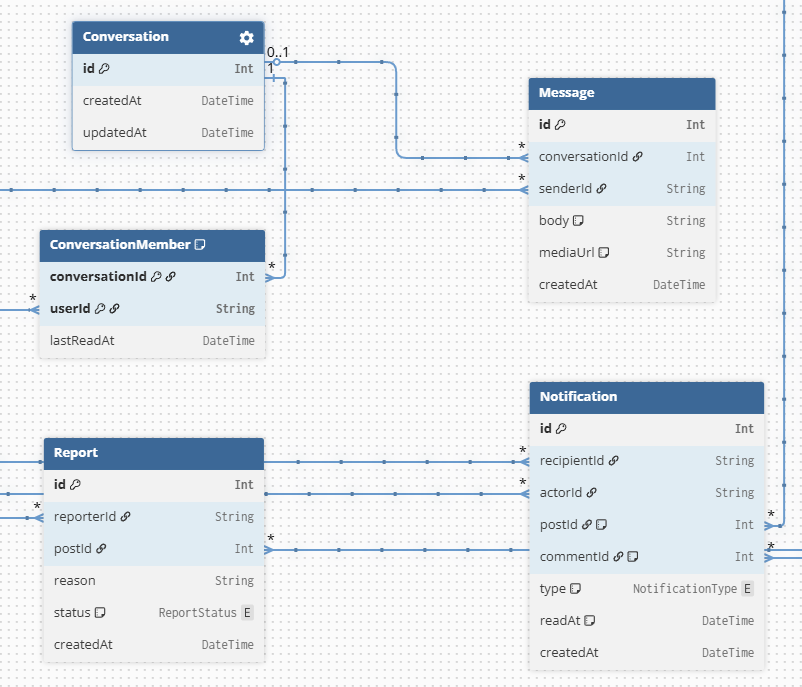
\includegraphics[width=0.92\linewidth,height=0.82\textheight,keepaspectratio]{images/image22.png}
  \caption{Communication -- Related Tables}
  \label{fig:18}
\end{figure}

\begin{longtable}{|p{0.45\linewidth}|p{0.45\linewidth}|}
\caption{Communication Tables} \label{tab:21} \\
\hline
\textbf{\textbullet  Conversation}\newline Description: Represents a single 1-to-1 Direct Message thread between two users. A conversation is created once and reused for all subsequent messages between the same pair.\newline Fields:\newline id (PK, Int)\newline createdAt (DateTime)\newline updatedAt (DateTime) Bumped on every new message; used to sort inbox by latest activity\newline Relationships:\newline One-to-Many with ConversationMember, Message & \textbf{\textbullet  ConversationMember}\newline Description: Junction table linking Users to Conversations. Tracks each participant's last-read timestamp, which powers the unread message badge count.\newline Fields:\newline conversationId (PK, FK, Int)\newline userId (PK, FK, String)\newline lastReadAt (DateTime, default: now()) Messages newer than this are considered "unread"\newline Relationships:\newline Composite PK ensures a user appears only once per conversation.\newline Many-to-One to Conversation, User \\
\hline
\endfirsthead
\multicolumn{2}{l}{\textit{(Continued from previous page)}} \\
\hline
\textbf{\textbullet  Conversation}\newline Description: Represents a single 1-to-1 Direct Message thread between two users. A conversation is created once and reused for all subsequent messages between the same pair.\newline Fields:\newline id (PK, Int)\newline createdAt (DateTime)\newline updatedAt (DateTime) Bumped on every new message; used to sort inbox by latest activity\newline Relationships:\newline One-to-Many with ConversationMember, Message & \textbf{\textbullet  ConversationMember}\newline Description: Junction table linking Users to Conversations. Tracks each participant's last-read timestamp, which powers the unread message badge count.\newline Fields:\newline conversationId (PK, FK, Int)\newline userId (PK, FK, String)\newline lastReadAt (DateTime, default: now()) Messages newer than this are considered "unread"\newline Relationships:\newline Composite PK ensures a user appears only once per conversation.\newline Many-to-One to Conversation, User \\
\hline
\endhead
\hline \multicolumn{2}{r}{\textit{Continued on next page}} \\
\endfoot
\hline
\endlastfoot
\textbullet  Message\newline Description: Individual message sent within a Conversation. Delivered in real-time via Socket.IO. Supports text and media attachments.\newline Fields:\newline id (PK, Int)\newline conversationId (FK, Int)\newline senderId (FK, String)\newline body (String, nullable, max 1000) Text content\newline mediaUrl (String, nullable) Image/file attachment URL\newline createdAt (DateTime)\newline Relationships:\newline Many-to-One with Conversation, User & \textbullet  Notification\newline Description: System-generated alert delivered to a recipient user when a relevant action occurs. Pushed in real-time via Socket.IO and persisted for the inbox view.\newline Fields:\newline id (PK, Int)\newline recipientId (FK, String)\newline actorId (FK, String)\newline type (Enum: LIKE | REPLY | REPOST | FOLLOW | MENTION | COMMUNITY\_POST | COMMUNITY\_NEW\_POST | COMMUNITY\_MOD\_ADDED | REPORT)\newline postId (FK, Int, nullable)\newline commentId (FK, Int, nullable)\newline readAt (DateTime, nullable)\newline createdAt (DateTime)\newline Relationships:\newline Many-to-One with User (recipient + actor), Post, Comment \\
\hline
\textbullet  Report\newline Description: Content flagging system. Any user can submit a report against a Post. System Admins review the report queue\newline Fields:\newline id (PK, Int)\newline reporterId (FK, String) --- The user who submitted the report\newline postId (FK, Int) --- The flagged post\newline reason (String) Report reason text (e.g., "Spam", "Hate speech")\newline status (Enum: OPEN | CLOSED, default: OPEN)\newline createdAt (DateTime)\newline Relationships:\newline Many-to-One with User (reporter), Post &  \\
\hline
\end{longtable}


\subsubsection{Class Diagram:}
\begin{figure}[H]
  \centering
  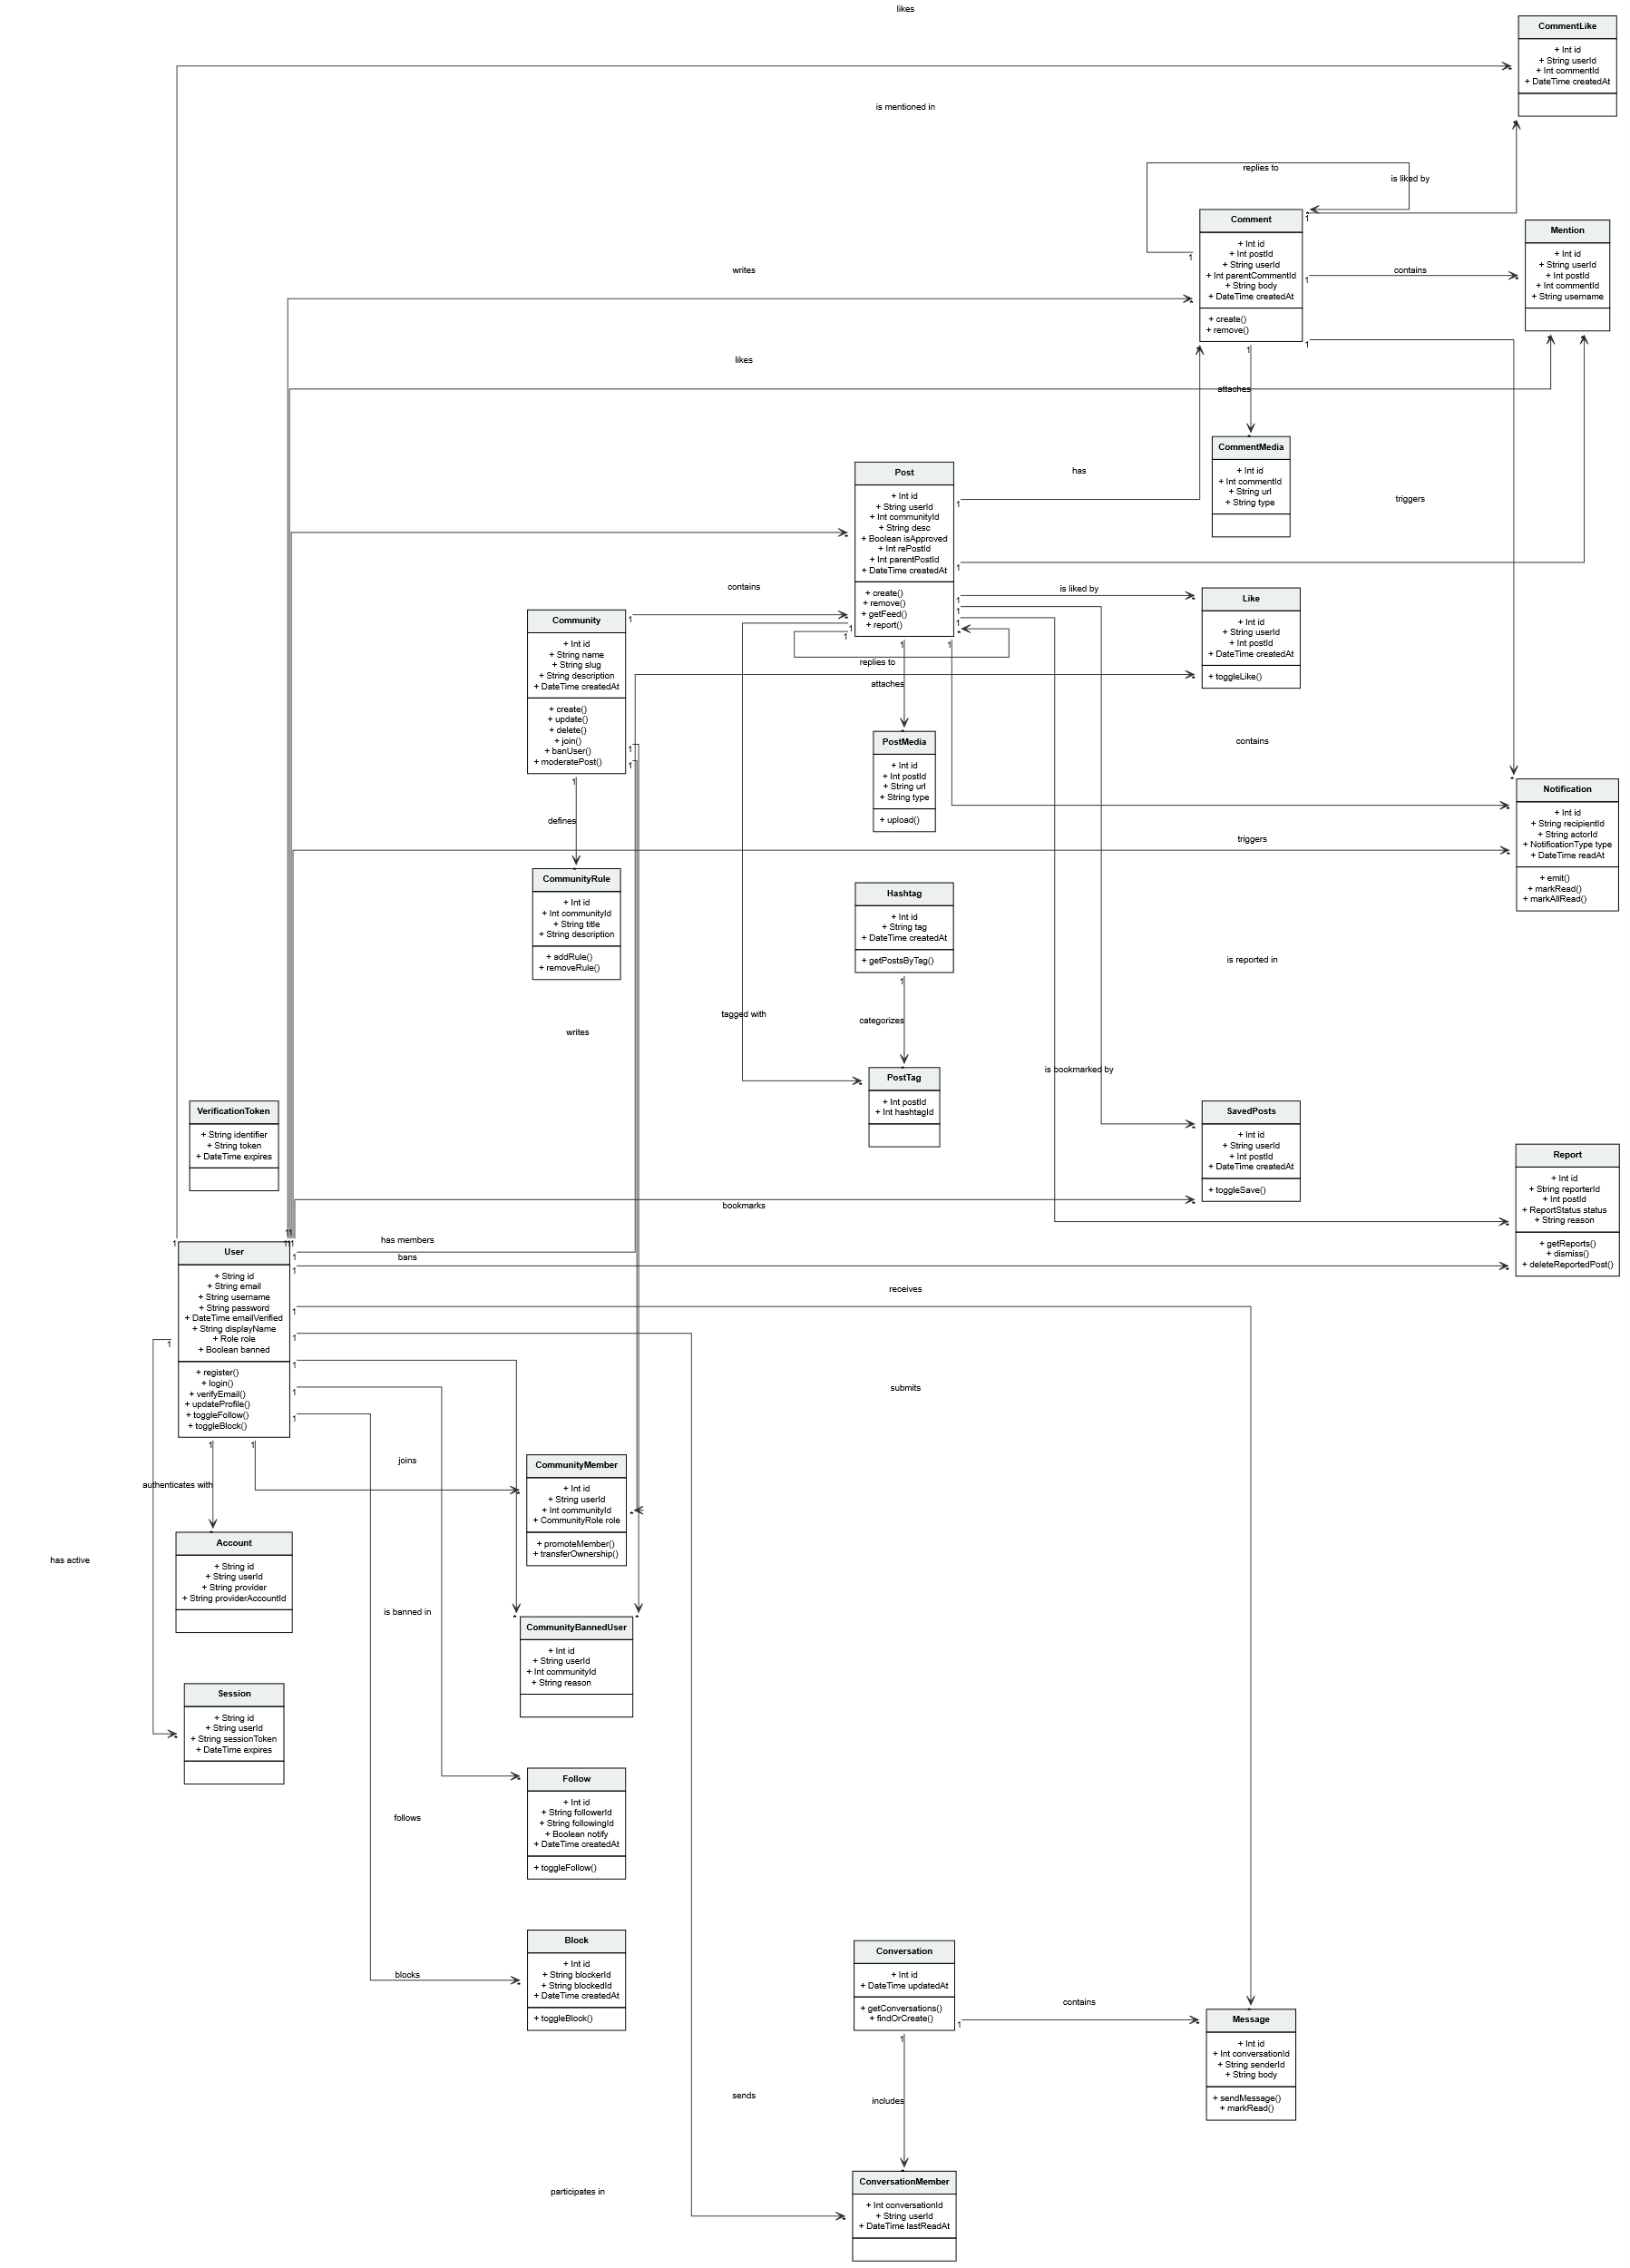
\includegraphics[width=0.92\linewidth,height=0.82\textheight,keepaspectratio]{images/image23.png}
  \caption{Class Diagram}
  \label{fig:19}
\end{figure}

Summary:
\begin{enumerate}
  \item Identity \& Access Domain Classes
\end{enumerate}

\begin{longtable}{|p{0.45\linewidth}|p{0.45\linewidth}|}
\caption{Identity \& Access Domain Classes} \label{tab:22} \\
\hline
\textbf{User}\newline Description: Core entity representing every platform account, storing identity and system-level access state.\newline Attributes:\newline id: String (PK)\newline email: String\newline username: String\newline password: String\newline emailVerified: DateTime\newline displayName: String\newline role: Role\newline banned: Boolean\newline Key Methods:\newline register(): Registers a new user\newline login(): Authenticates the user\newline verifyEmail(): Verifies email address\newline updateProfile(): Updates profile details\newline toggleFollow(): Follows or unfollows another user\newline toggleBlock(): Blocks or unblocks another user\newline Relationships:\newline Composition -> Account (one-to-many)\newline Composition -> Session (one-to-many)\newline Association -> Follow\newline Association -> Block\newline Association-> CommunityMember\newline Association -> Post\newline Association -> Comment\newline Association -> Notification & \textbf{VerificationToken}\newline Description: Stores single-use OTP codes for email verification and password reset.\newline Attributes:\newline identifier: String (PK)\newline token: String\newline expires: DateTime\newline Key Methods: None\newline Relationships: None \\
\hline
\endfirsthead
\multicolumn{2}{l}{\textit{(Continued from previous page)}} \\
\hline
\textbf{User}\newline Description: Core entity representing every platform account, storing identity and system-level access state.\newline Attributes:\newline id: String (PK)\newline email: String\newline username: String\newline password: String\newline emailVerified: DateTime\newline displayName: String\newline role: Role\newline banned: Boolean\newline Key Methods:\newline register(): Registers a new user\newline login(): Authenticates the user\newline verifyEmail(): Verifies email address\newline updateProfile(): Updates profile details\newline toggleFollow(): Follows or unfollows another user\newline toggleBlock(): Blocks or unblocks another user\newline Relationships:\newline Composition -> Account (one-to-many)\newline Composition -> Session (one-to-many)\newline Association -> Follow\newline Association -> Block\newline Association-> CommunityMember\newline Association -> Post\newline Association -> Comment\newline Association -> Notification & \textbf{VerificationToken}\newline Description: Stores single-use OTP codes for email verification and password reset.\newline Attributes:\newline identifier: String (PK)\newline token: String\newline expires: DateTime\newline Key Methods: None\newline Relationships: None \\
\hline
\endhead
\hline \multicolumn{2}{r}{\textit{Continued on next page}} \\
\endfoot
\hline
\endlastfoot
\end{longtable}

\begin{enumerate}
  \item Content Domain Classes
\end{enumerate}

\begin{longtable}{|p{0.45\linewidth}|p{0.45\linewidth}|}
\caption{Content Domain Classes} \label{tab:23} \\
\hline
\textbf{Post}\newline Description: Represents original posts, reposts, and quote-reposts.\newline Attributes:\newline id: Int (PK)\newline userId: String (FK)\newline communityId: Int (FK)\newline desc: String\newline isApproved: Boolean\newline rePostId: Int (FK)\newline parentPostId: Int (FK)\newline createdAt: DateTime\newline Key Methods:\newline create(): Creates a new post\newline remove(): Soft deletes the post\newline getFeed(): Retrieves post feed\newline report(): Reports the post\newline Relationships:\newline Association -> User\newline Association -> Community\newline Composition -> PostMedia (one-to-many)\newline Composition -> Comment (one-to-many)\newline Association -> PostTag (one-to-many) & \textbf{Comment}\newline Description: User replies to a Post, supporting nested comment threads.\newline Attributes:\newline id: Int (PK)\newline postId: Int (FK)\newline userId: String (FK)\newline parentCommentId: Int (FK)\newline body: String\newline createdAt: DateTime\newline Key Methods:\newline create(): Adds a comment\newline remove(): Removes a comment\newline Relationships:\newline Association -> User\newline Association -> Post\newline Composition -> CommentMedia (one-to-many) \\
\hline
\endfirsthead
\multicolumn{2}{l}{\textit{(Continued from previous page)}} \\
\hline
\textbf{Post}\newline Description: Represents original posts, reposts, and quote-reposts.\newline Attributes:\newline id: Int (PK)\newline userId: String (FK)\newline communityId: Int (FK)\newline desc: String\newline isApproved: Boolean\newline rePostId: Int (FK)\newline parentPostId: Int (FK)\newline createdAt: DateTime\newline Key Methods:\newline create(): Creates a new post\newline remove(): Soft deletes the post\newline getFeed(): Retrieves post feed\newline report(): Reports the post\newline Relationships:\newline Association -> User\newline Association -> Community\newline Composition -> PostMedia (one-to-many)\newline Composition -> Comment (one-to-many)\newline Association -> PostTag (one-to-many) & \textbf{Comment}\newline Description: User replies to a Post, supporting nested comment threads.\newline Attributes:\newline id: Int (PK)\newline postId: Int (FK)\newline userId: String (FK)\newline parentCommentId: Int (FK)\newline body: String\newline createdAt: DateTime\newline Key Methods:\newline create(): Adds a comment\newline remove(): Removes a comment\newline Relationships:\newline Association -> User\newline Association -> Post\newline Composition -> CommentMedia (one-to-many) \\
\hline
\endhead
\hline \multicolumn{2}{r}{\textit{Continued on next page}} \\
\endfoot
\hline
\endlastfoot
PostMedia\newline Description: Stores image and video attachments for a Post.\newline Attributes:\newline id: Int (PK)\newline postId: Int (FK)\newline url: String\newline type: String\newline Key Methods:\newline upload(): Uploads media file\newline Relationships:\newline Association -> Post & CommentMedia\newline Description: File attachments embedded inside comments.\newline Attributes:\newline id: Int (PK)\newline commentId: Int (FK)\newline url: String\newline type: String\newline Relationships:\newline Association -> Comment \\
\hline
Hashtag \& PostTag\newline Description: Registry of tags and the junction class link Posts to Hashtags.\newline Key Methods:\newline getPostsByTag(): Retrieves posts by hashtag\newline Relationships:\newline Association -> Post &  \\
\hline
\end{longtable}

\begin{enumerate}
  \item Social Engagement Domain Classes
\end{enumerate}

\begin{longtable}{|p{0.45\linewidth}|p{0.45\linewidth}|}
\caption{Social Engagement Domain Classes} \label{tab:24} \\
\hline
\textbf{Follow}\newline Description: Directed social graph edge for user following.\newline Attributes:\newline id: Int (PK)\newline followerId: String (FK)\newline followingId: String (FK)\newline notify: Boolean\newline createdAt: DateTime\newline Key Methods:\newline toggleFollow(): Follows/unfollows\newline Relationships:\newline Association -> User & \textbf{Like}\newline Description: Records a User's reaction on a Post.\newline Attributes:\newline id: Int (PK)\newline userId: String (FK)\newline postId: Int (FK)\newline createdAt: DateTime\newline Key Methods:\newline toggleLike(): Likes/ unlikes a post\newline Relationships:\newline Association -> User\newline Association -> Post \\
\hline
\endfirsthead
\multicolumn{2}{l}{\textit{(Continued from previous page)}} \\
\hline
\textbf{Follow}\newline Description: Directed social graph edge for user following.\newline Attributes:\newline id: Int (PK)\newline followerId: String (FK)\newline followingId: String (FK)\newline notify: Boolean\newline createdAt: DateTime\newline Key Methods:\newline toggleFollow(): Follows/unfollows\newline Relationships:\newline Association -> User & \textbf{Like}\newline Description: Records a User's reaction on a Post.\newline Attributes:\newline id: Int (PK)\newline userId: String (FK)\newline postId: Int (FK)\newline createdAt: DateTime\newline Key Methods:\newline toggleLike(): Likes/ unlikes a post\newline Relationships:\newline Association -> User\newline Association -> Post \\
\hline
\endhead
\hline \multicolumn{2}{r}{\textit{Continued on next page}} \\
\endfoot
\hline
\endlastfoot
Block\newline Description: Mutual blacklist between two users.\newline Attributes:\newline id: Int (PK)\newline blockerId: String (FK)\newline blockedId: String (FK)\newline createdAt: DateTime\newline Key Methods:\newline toggleBlock(): Blocks or unblocks a user\newline Relationships:\newline Association -> User & SavedPost\newline Description: User's personal bookmark list.\newline Attributes:\newline id: Int (PK)\newline userId: String (FK)\newline postId: Int (FK)\newline createdAt: DateTime\newline Key Methods:\newline toggleSave(): Save/unsave a post\newline Relationships:\newline Association -> User\newline Association -> Post \\
\hline
Mention\newline Description: Records @username tags inside content.\newline Attributes:\newline id: Int (PK)\newline userId: String (FK)\newline postId: Int (FK)\newline commentId: Int (FK)\newline username: String\newline Relationships:\newline Association -> User, Post, Comment & CommentLike\newline Description: Records a User's reaction on a Comment.\newline Attributes:\newline id: Int (PK)\newline userId: String (FK)\newline commentID: Int (FK)\newline Relationships:\newline Association -> User\newline Association -> Comment \\
\hline
\end{longtable}

\begin{enumerate}
  \item Community \& Moderation Domain Classes
\end{enumerate}

\begin{longtable}{|p{0.45\linewidth}|p{0.45\linewidth}|}
\caption{Community \& Moderation Domain Classes} \label{tab:25} \\
\hline
\textbf{Community}\newline Description: A shared space for members with a common interest.\newline Attributes:\newline id: Int (PK)\newline name: String\newline slug: String\newline description: String\newline createdAt: DateTime\newline Key Methods:\newline create(): Creates a new community\newline update(): Update community detail\newline delete(): Deletes the community\newline join(): Joins/ leaves the community\newline banUser(): Bans a user from the community\newline moderatePost(): Approves/rejects a post\newline Relationships:\newline Composition -> CommunityMember\newline Composition -> CommunityRule\newline Composition-> CommunityBannedUser\newline Composition -> Post & \textbf{CommunityMember}\newline Description: Manages community members and their roles.\newline Attributes:\newline id: Int (PK)\newline userId: String (FK)\newline communityId: Int (FK)\newline role: CommunityRole\newline Key Methods:\newline promoteMember(): Promotes a member to moderator\newline transferOwnership(): Transfers community ownership\newline Relationships:\newline Association -> Community\newline Association -> User \\
\hline
\endfirsthead
\multicolumn{2}{l}{\textit{(Continued from previous page)}} \\
\hline
\textbf{Community}\newline Description: A shared space for members with a common interest.\newline Attributes:\newline id: Int (PK)\newline name: String\newline slug: String\newline description: String\newline createdAt: DateTime\newline Key Methods:\newline create(): Creates a new community\newline update(): Update community detail\newline delete(): Deletes the community\newline join(): Joins/ leaves the community\newline banUser(): Bans a user from the community\newline moderatePost(): Approves/rejects a post\newline Relationships:\newline Composition -> CommunityMember\newline Composition -> CommunityRule\newline Composition-> CommunityBannedUser\newline Composition -> Post & \textbf{CommunityMember}\newline Description: Manages community members and their roles.\newline Attributes:\newline id: Int (PK)\newline userId: String (FK)\newline communityId: Int (FK)\newline role: CommunityRole\newline Key Methods:\newline promoteMember(): Promotes a member to moderator\newline transferOwnership(): Transfers community ownership\newline Relationships:\newline Association -> Community\newline Association -> User \\
\hline
\endhead
\hline \multicolumn{2}{r}{\textit{Continued on next page}} \\
\endfoot
\hline
\endlastfoot
CommunityBannedUser\newline Description: Community-level blacklist enforced by Moderators.\newline Attributes:\newline id: Int (PK)\newline userId: String (FK)\newline communityId: Int (FK)\newline reason: String\newline Relationships:\newline Association -> User\newline Association -> Community & CommunityRule\newline Description: Custom rules set by the community.\newline Attributes:\newline id: Int (PK)\newline communityId: Int (FK)\newline title: String\newline description: String\newline Key Methods:\newline addRule(): Adds a new rule\newline removeRule(): Removes a rule\newline Relationships\newline Association -> Community \\
\hline
\end{longtable}

\begin{enumerate}
  \item Communication Domain Classes
\end{enumerate}

\begin{longtable}{|p{0.45\linewidth}|p{0.45\linewidth}|}
\caption{Communication Domain Classes} \label{tab:26} \\
\hline
\textbf{ShopOrder}\newline Description: Represents a direct message thread.\newline Attributes:\newline id: Int (PK)\newline updateAt: DateTime\newline Key Methods:\newline getConversations(): Retrieves user conversations\newline findOrCreate(): Finds or creates a conversation thread\newline Relationships:\newline Composition -> ConversationMember (one-to-many)\newline Composition -> Message (one-to-many) & \textbf{Notification}\newline Description: System-generated alert\newline Attributes:\newline id: Int (PK)\newline recipientId: String (FK)\newline actorId: String (FK)\newline type: NotificationType\newline readAt: DateTime\newline Key Methods:\newline emit(): Emits real-time notification\newline markRead(): Marks notification\newline markAllRead(): Marks all notifications as read\newline Relationships:\newline Association -> User\newline Association -> Post\newline Association -> Comment \\
\hline
\endfirsthead
\multicolumn{2}{l}{\textit{(Continued from previous page)}} \\
\hline
\textbf{ShopOrder}\newline Description: Represents a direct message thread.\newline Attributes:\newline id: Int (PK)\newline updateAt: DateTime\newline Key Methods:\newline getConversations(): Retrieves user conversations\newline findOrCreate(): Finds or creates a conversation thread\newline Relationships:\newline Composition -> ConversationMember (one-to-many)\newline Composition -> Message (one-to-many) & \textbf{Notification}\newline Description: System-generated alert\newline Attributes:\newline id: Int (PK)\newline recipientId: String (FK)\newline actorId: String (FK)\newline type: NotificationType\newline readAt: DateTime\newline Key Methods:\newline emit(): Emits real-time notification\newline markRead(): Marks notification\newline markAllRead(): Marks all notifications as read\newline Relationships:\newline Association -> User\newline Association -> Post\newline Association -> Comment \\
\hline
\endhead
\hline \multicolumn{2}{r}{\textit{Continued on next page}} \\
\endfoot
\hline
\endlastfoot
ConservationMember\newline Description: Junction class tracking conversation participants.\newline Attributes:\newline conversationId: Int (FK)\newline userId: String (FK)\newline lastReadAt: DateTime\newline Relationships:\newline Association -> User\newline Association -> Conversation & Report\newline Description: Content flagging system for moderation.\newline Attributes:\newline id: Int (PK)\newline reporterId: String (FK)\newline postId: Int (FK)\newline status: ReportStatus\newline reason: String\newline Key Methods:\newline getReports(): Retrieves list post\newline dismiss(): Dismisses a report\newline deleteReportedPost(): Deletes the reported post\newline Relationships:\newline Association -> User\newline Association -> Post \\
\hline
Message\newline Description: Individual message within a conversation.\newline Attributes:\newline id: Int (PK)\newline conversationId: Int (FK)\newline senderId: String (FK)\newline body: String\newline Key Methods:\newline sendMessage(): Sends a new message\newline markRead(): Marks message as read\newline Relationships:\newline Association -> User\newline Association -> Conservation &  \\
\hline
\end{longtable}


\subsubsection{Sequence Diagram}

This section presents ten sequence diagrams that model the dynamic behavior of the Breadit social network, mapping directly to its core use cases. These diagrams visualize the runtime interactions between the user, Next.js frontend, NestJS backend API, PostgreSQL database (via Prisma), and real-time Socket.IO/Redis pipeline. The illustrated flows cover: (1) Authentication, (2) Content Discovery, (3) Post Management, (4) Post Interaction, (5) Relationship Management, (6) Profile Management, (7) Direct Messaging, (8) Real-Time Notifications, (9) Community Management, and (10) Administrative Moderation.

\medskip\noindent\textbf{Authentication \& Account Management}\\[2pt]
\begin{figure}[H]
  \centering
  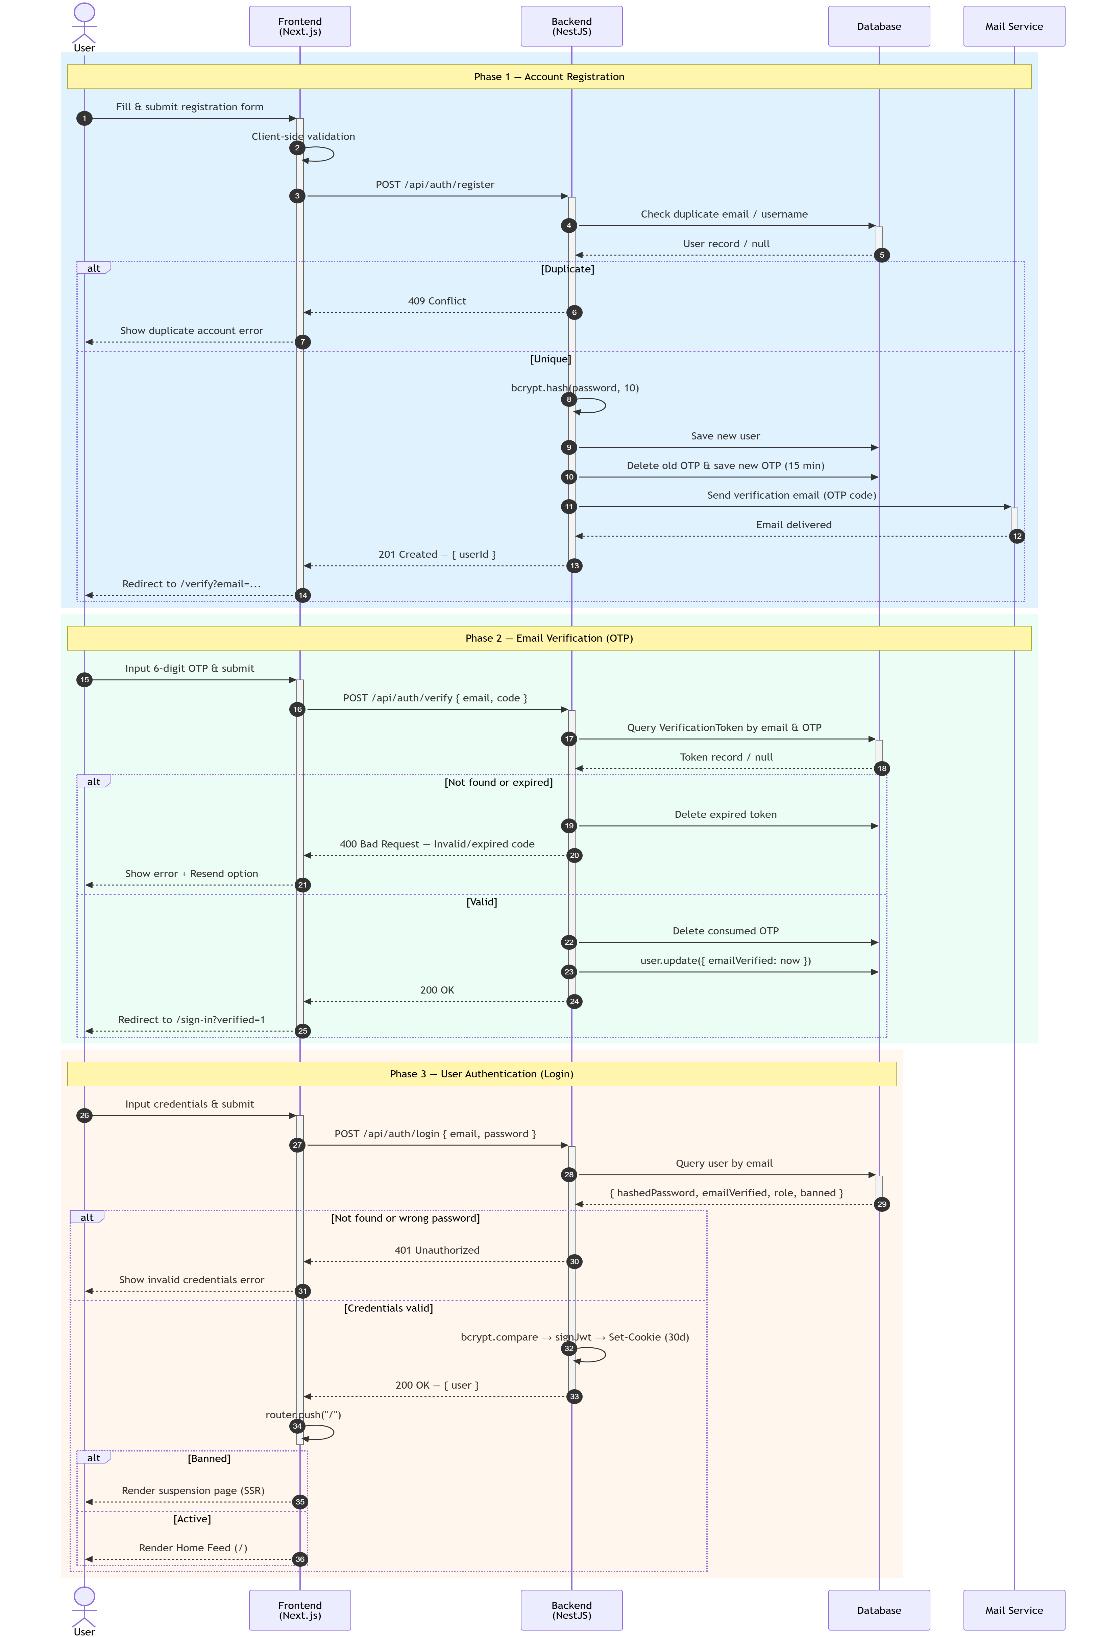
\includegraphics[width=0.92\linewidth,height=0.82\textheight,keepaspectratio]{images/image25.png}
  \caption{Authentication \& Account Management Diagram}
  \label{fig:20}
\end{figure}

\medskip\noindent\textbf{Feeds and Discovery}\\[2pt]
\begin{figure}[H]
  \centering
  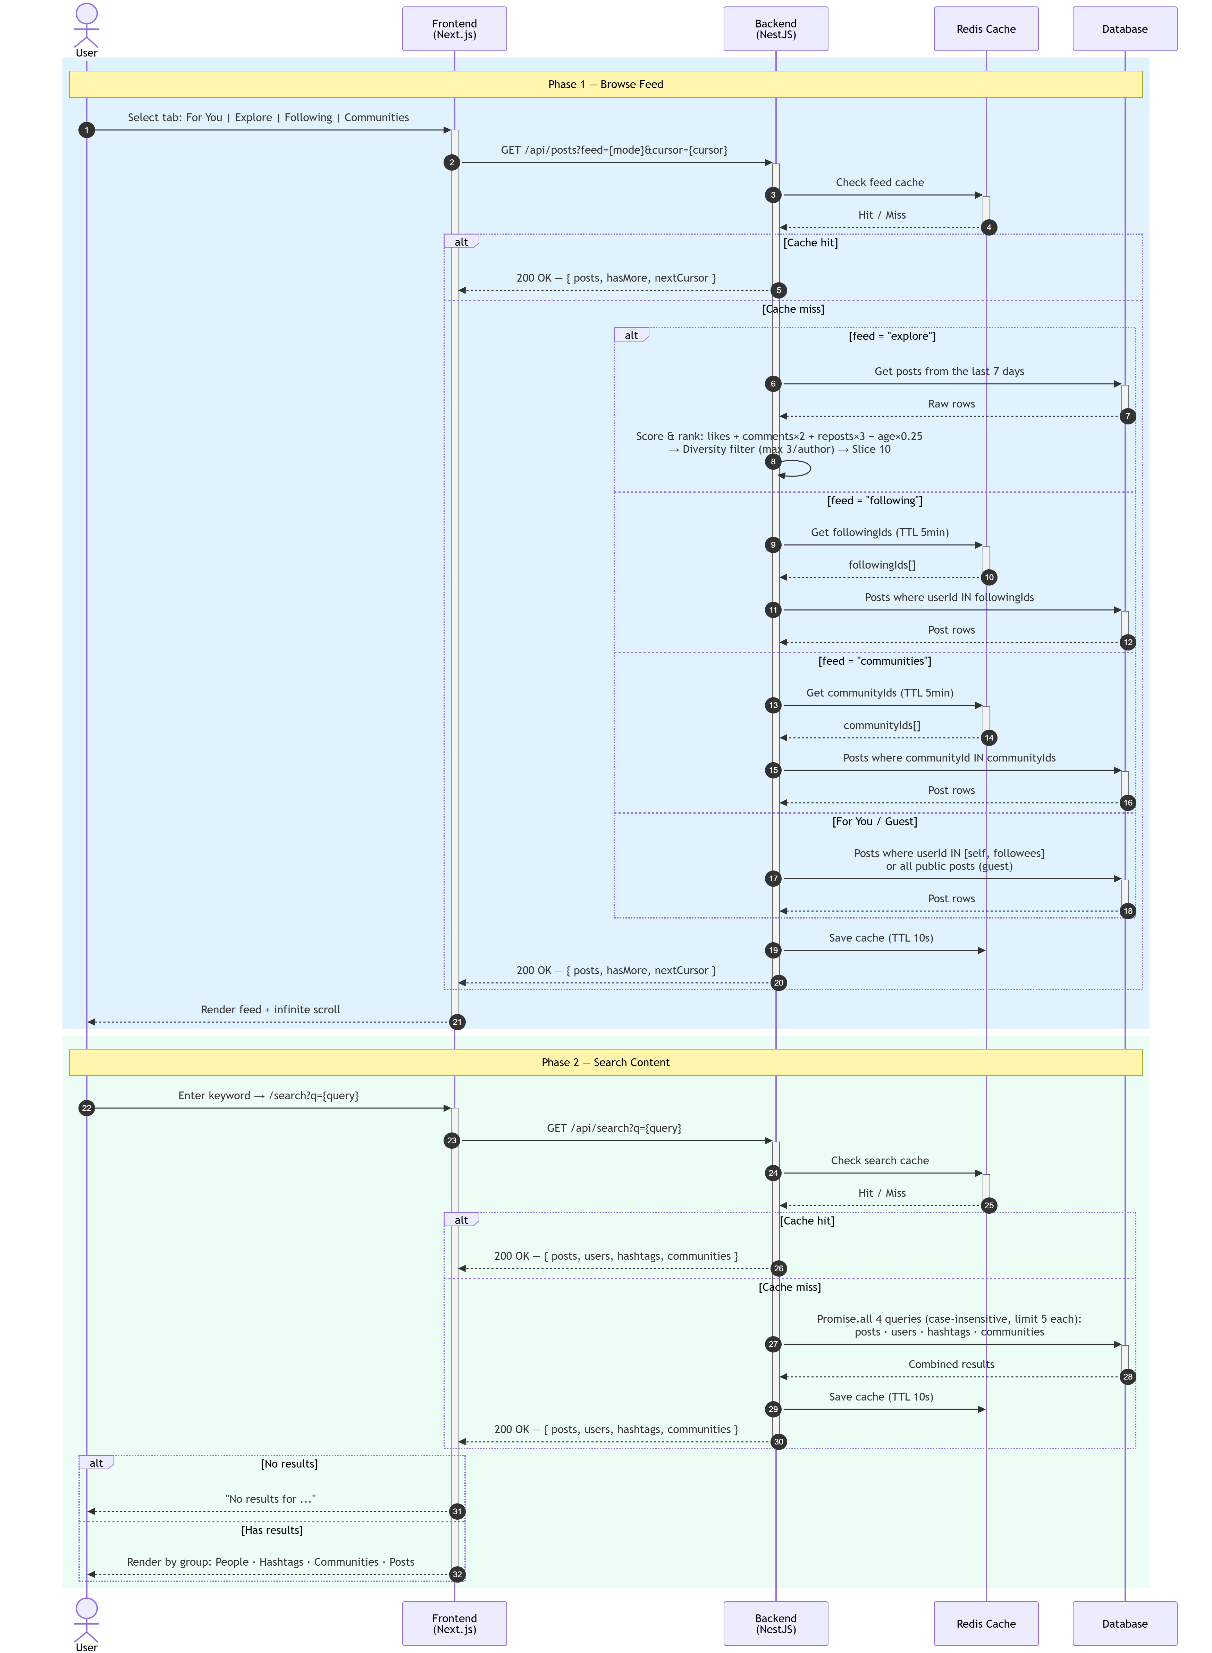
\includegraphics[width=0.92\linewidth,height=0.82\textheight,keepaspectratio]{images/image26.png}
  \caption{Feeds and Discovery Diagram}
  \label{fig:21}
\end{figure}

\medskip\noindent\textbf{Post Management}\\[2pt]
\begin{figure}[H]
  \centering
  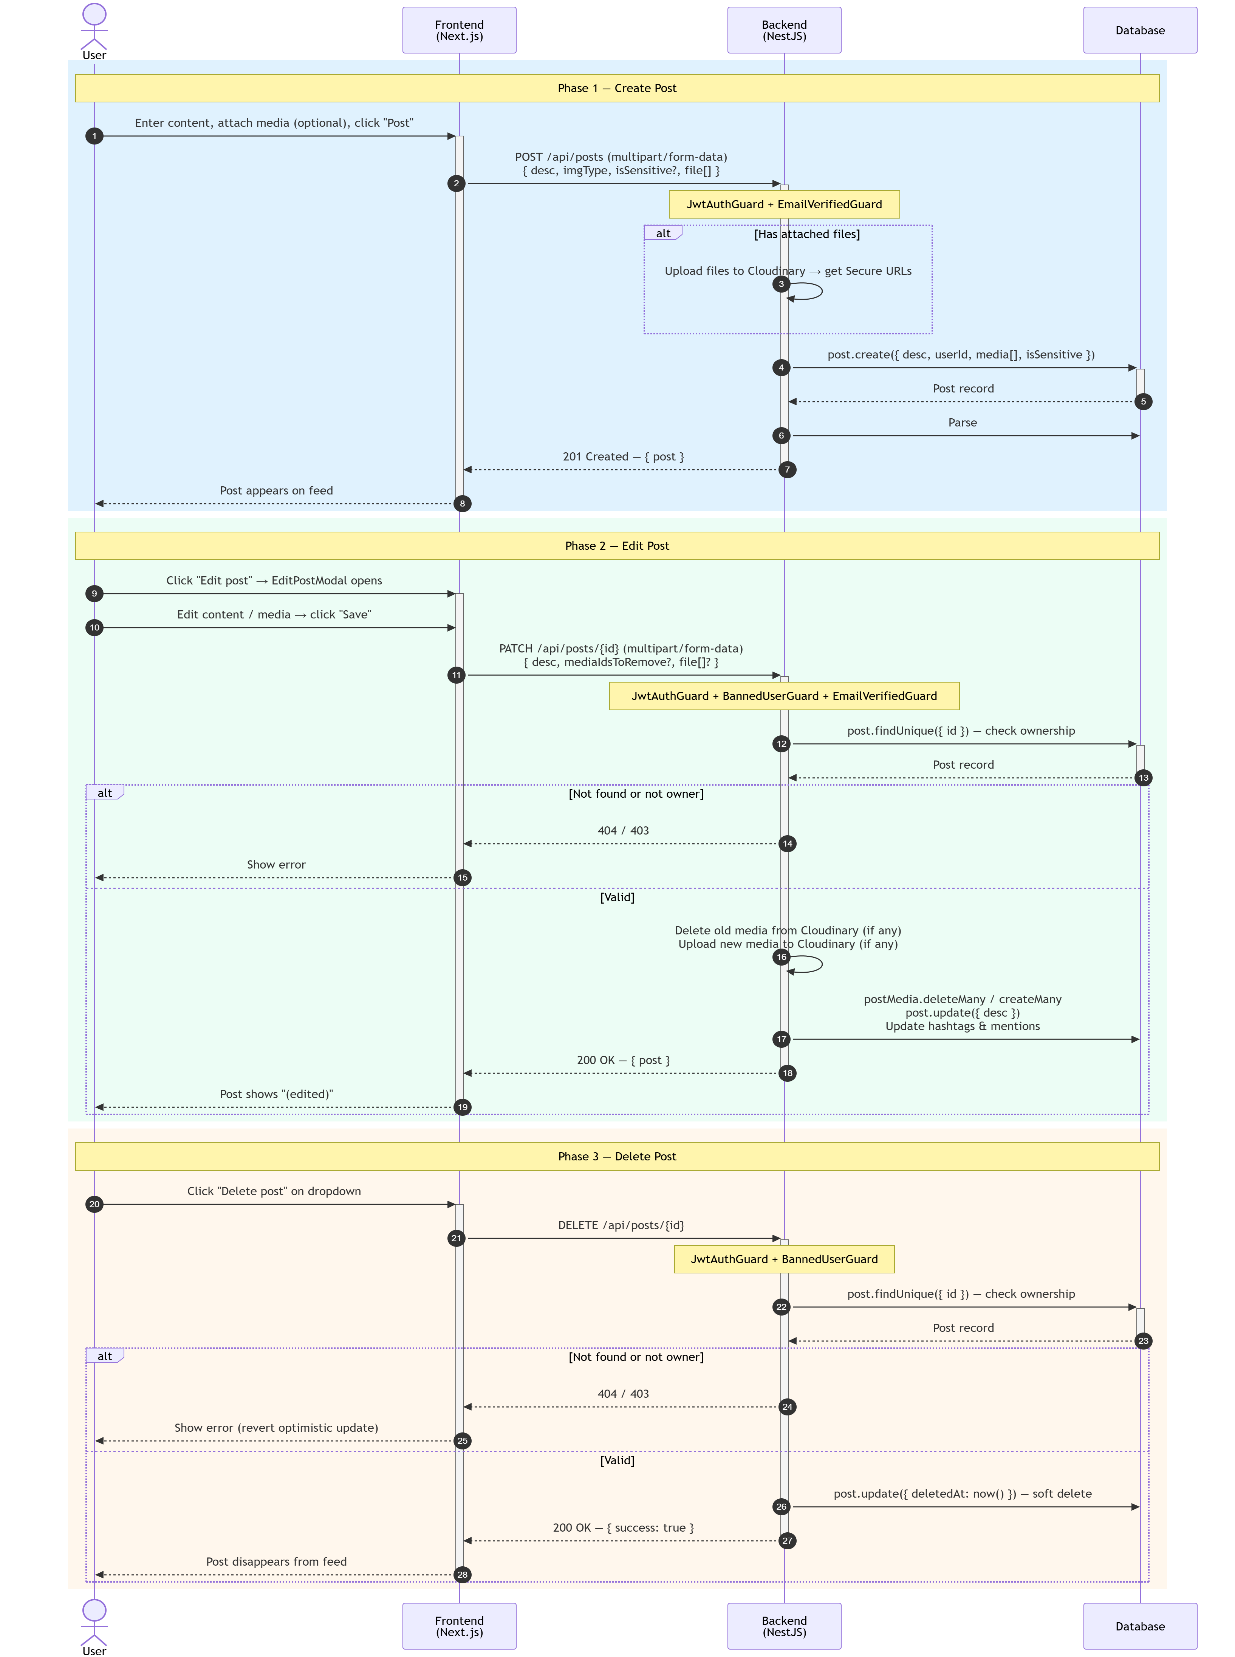
\includegraphics[width=0.92\linewidth,height=0.82\textheight,keepaspectratio]{images/image27.png}
  \caption{Post Management Diagram}
  \label{fig:22}
\end{figure}

\medskip\noindent\textbf{Post Interaction}\\[2pt]
\begin{figure}[H]
  \centering
  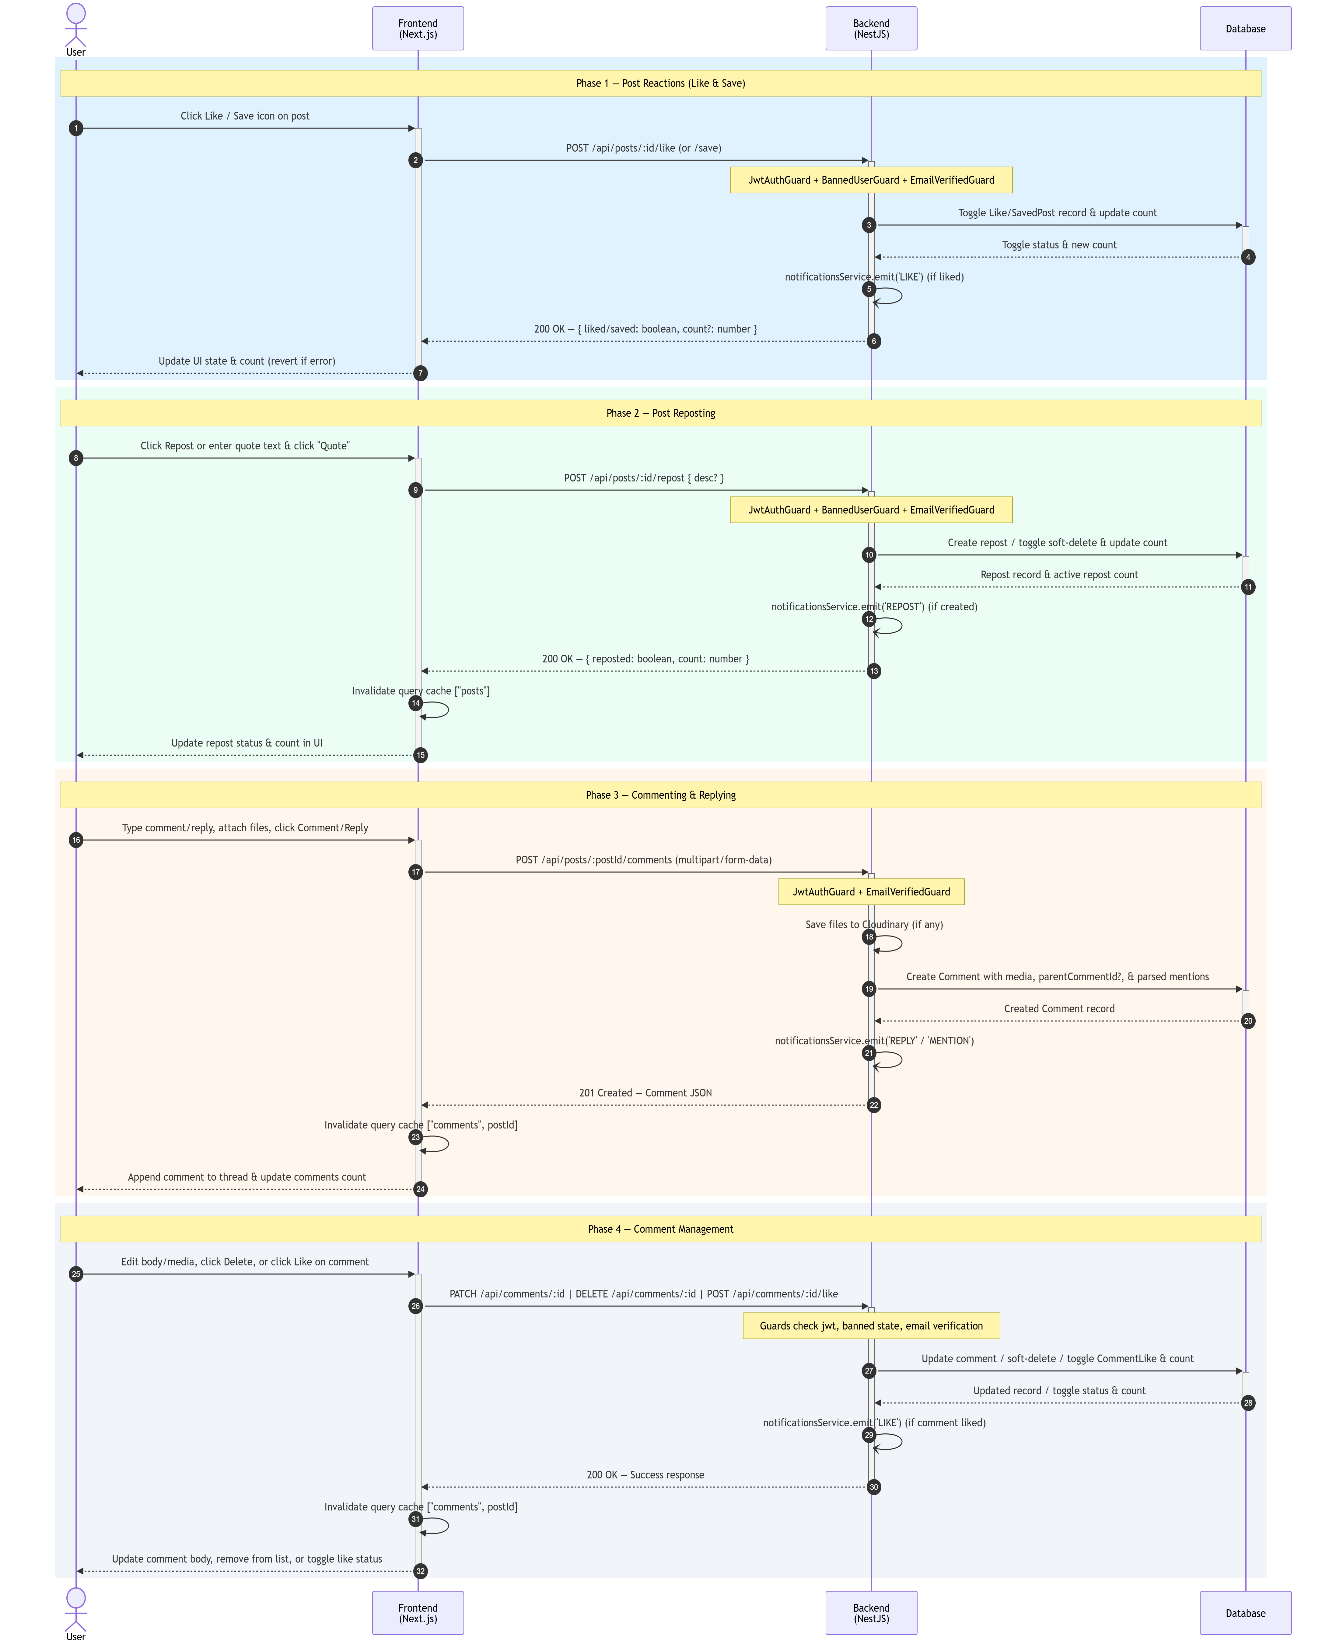
\includegraphics[width=0.92\linewidth,height=0.82\textheight,keepaspectratio]{images/image28.png}
  \caption{Post Interaction Diagram}
  \label{fig:23}
\end{figure}

\medskip\noindent\textbf{User Relationship Management}\\[2pt]
\begin{figure}[H]
  \centering
  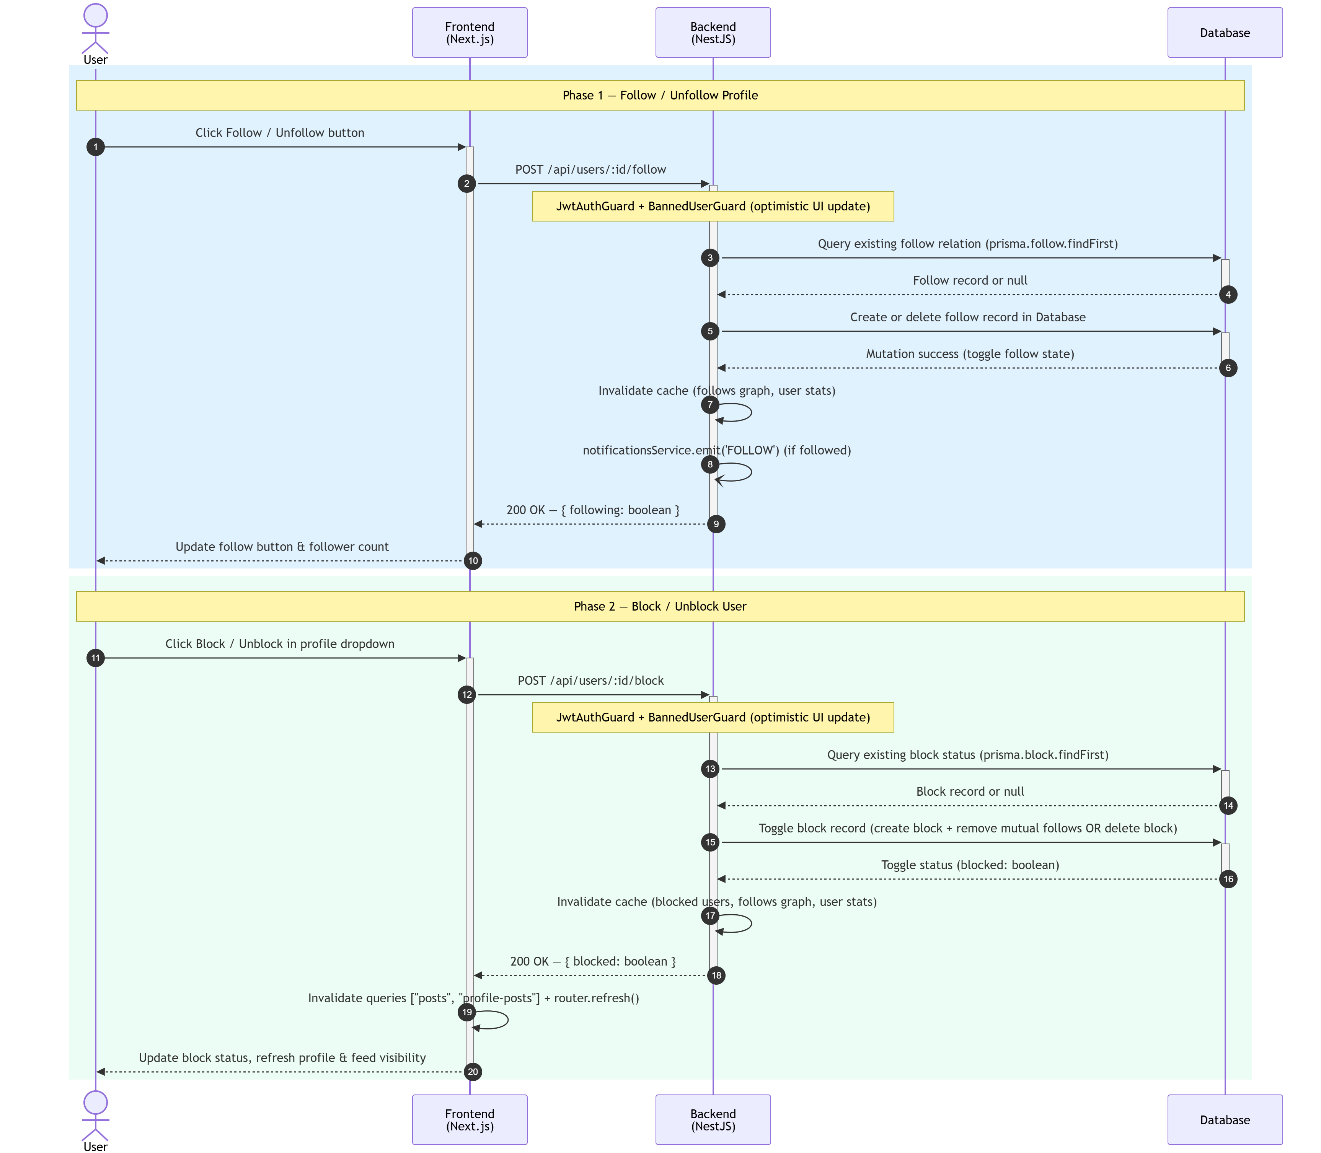
\includegraphics[width=0.92\linewidth,height=0.82\textheight,keepaspectratio]{images/image29.png}
  \caption{User Relationship Management Diagram}
  \label{fig:24}
\end{figure}

\medskip\noindent\textbf{User Profile Management}\\[2pt]
\begin{figure}[H]
  \centering
  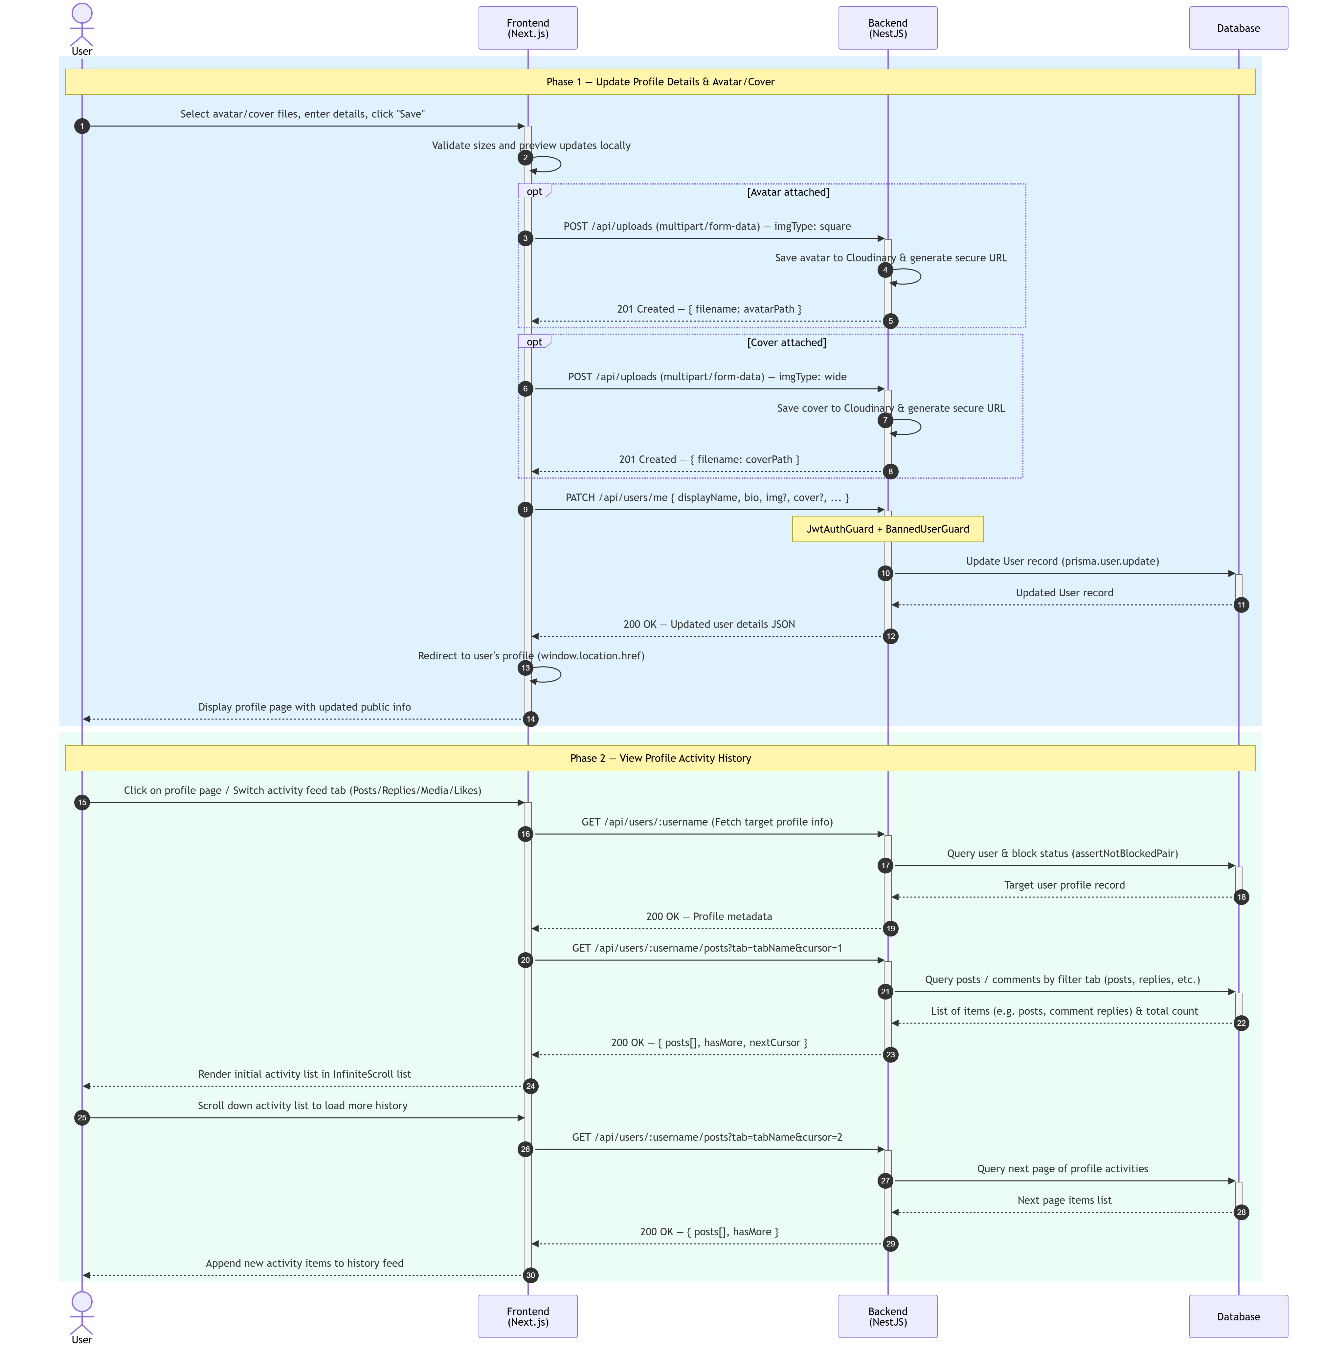
\includegraphics[width=0.92\linewidth,height=0.82\textheight,keepaspectratio]{images/image30.png}
  \caption{User Profile Management Diagram}
  \label{fig:25}
\end{figure}

\medskip\noindent\textbf{Direct Messaging}\\[2pt]
\begin{figure}[H]
  \centering
  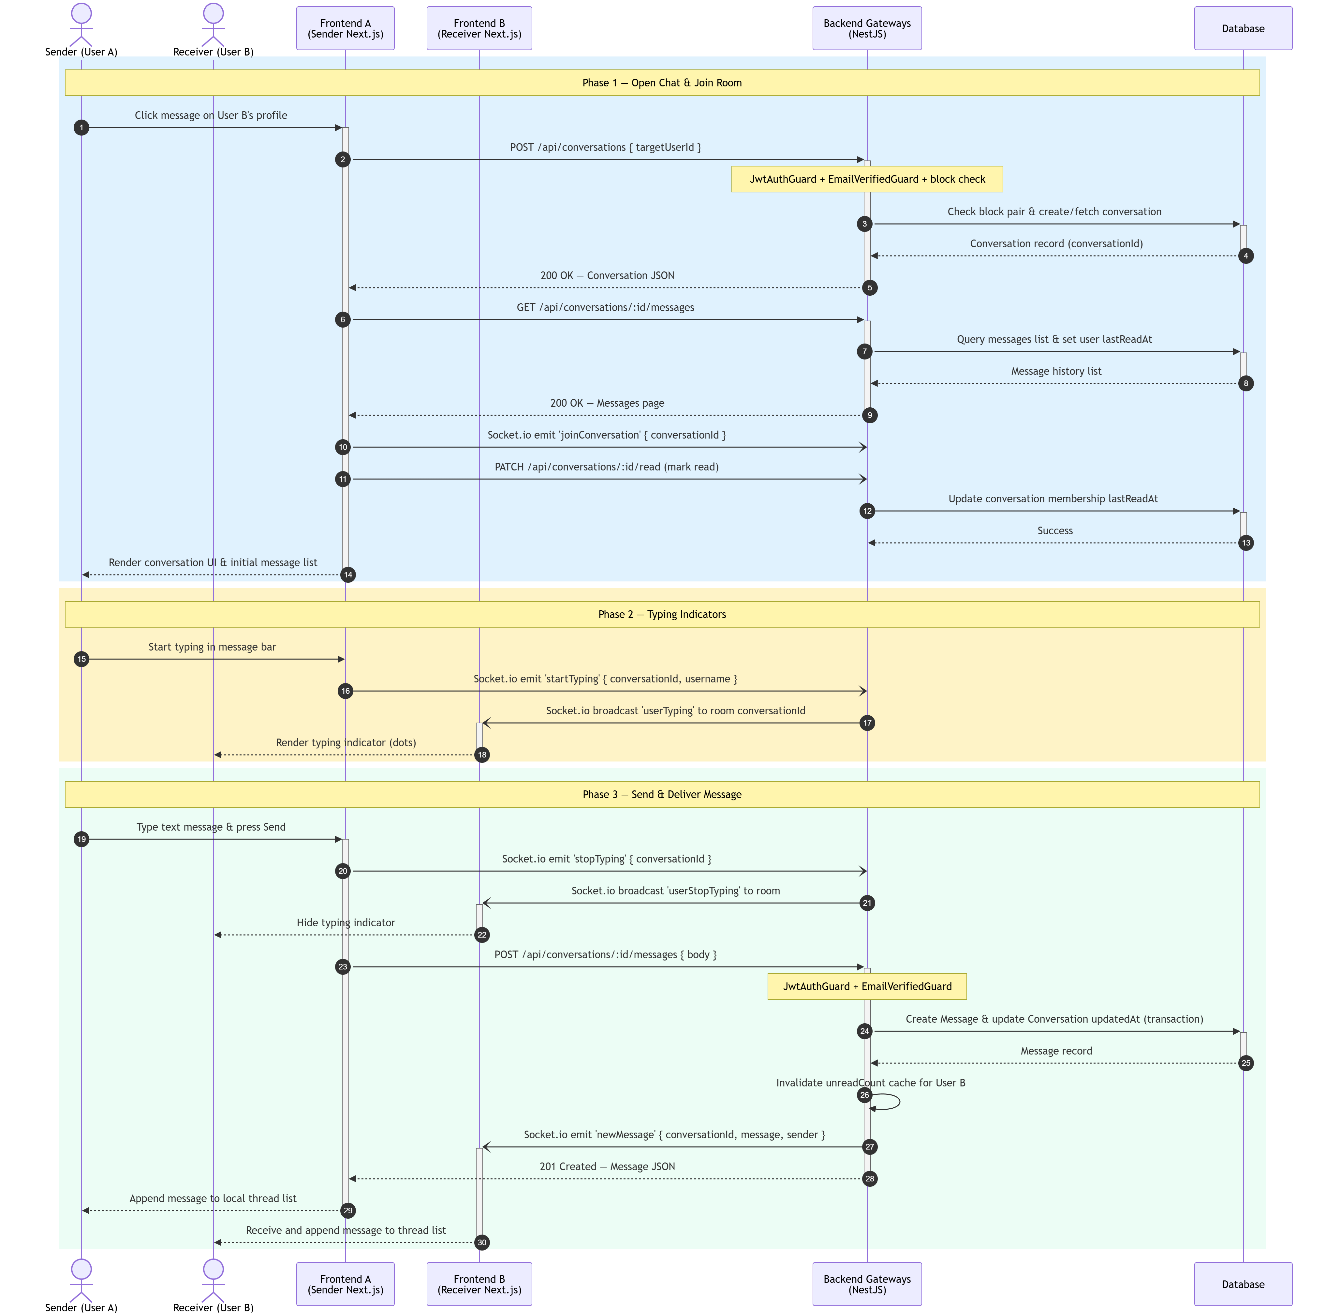
\includegraphics[width=0.92\linewidth,height=0.82\textheight,keepaspectratio]{images/image31.png}
  \caption{Direct Messaging Diagram}
  \label{fig:26}
\end{figure}

\medskip\noindent\textbf{Real-time Notifications}\\[2pt]
\begin{figure}[H]
  \centering
  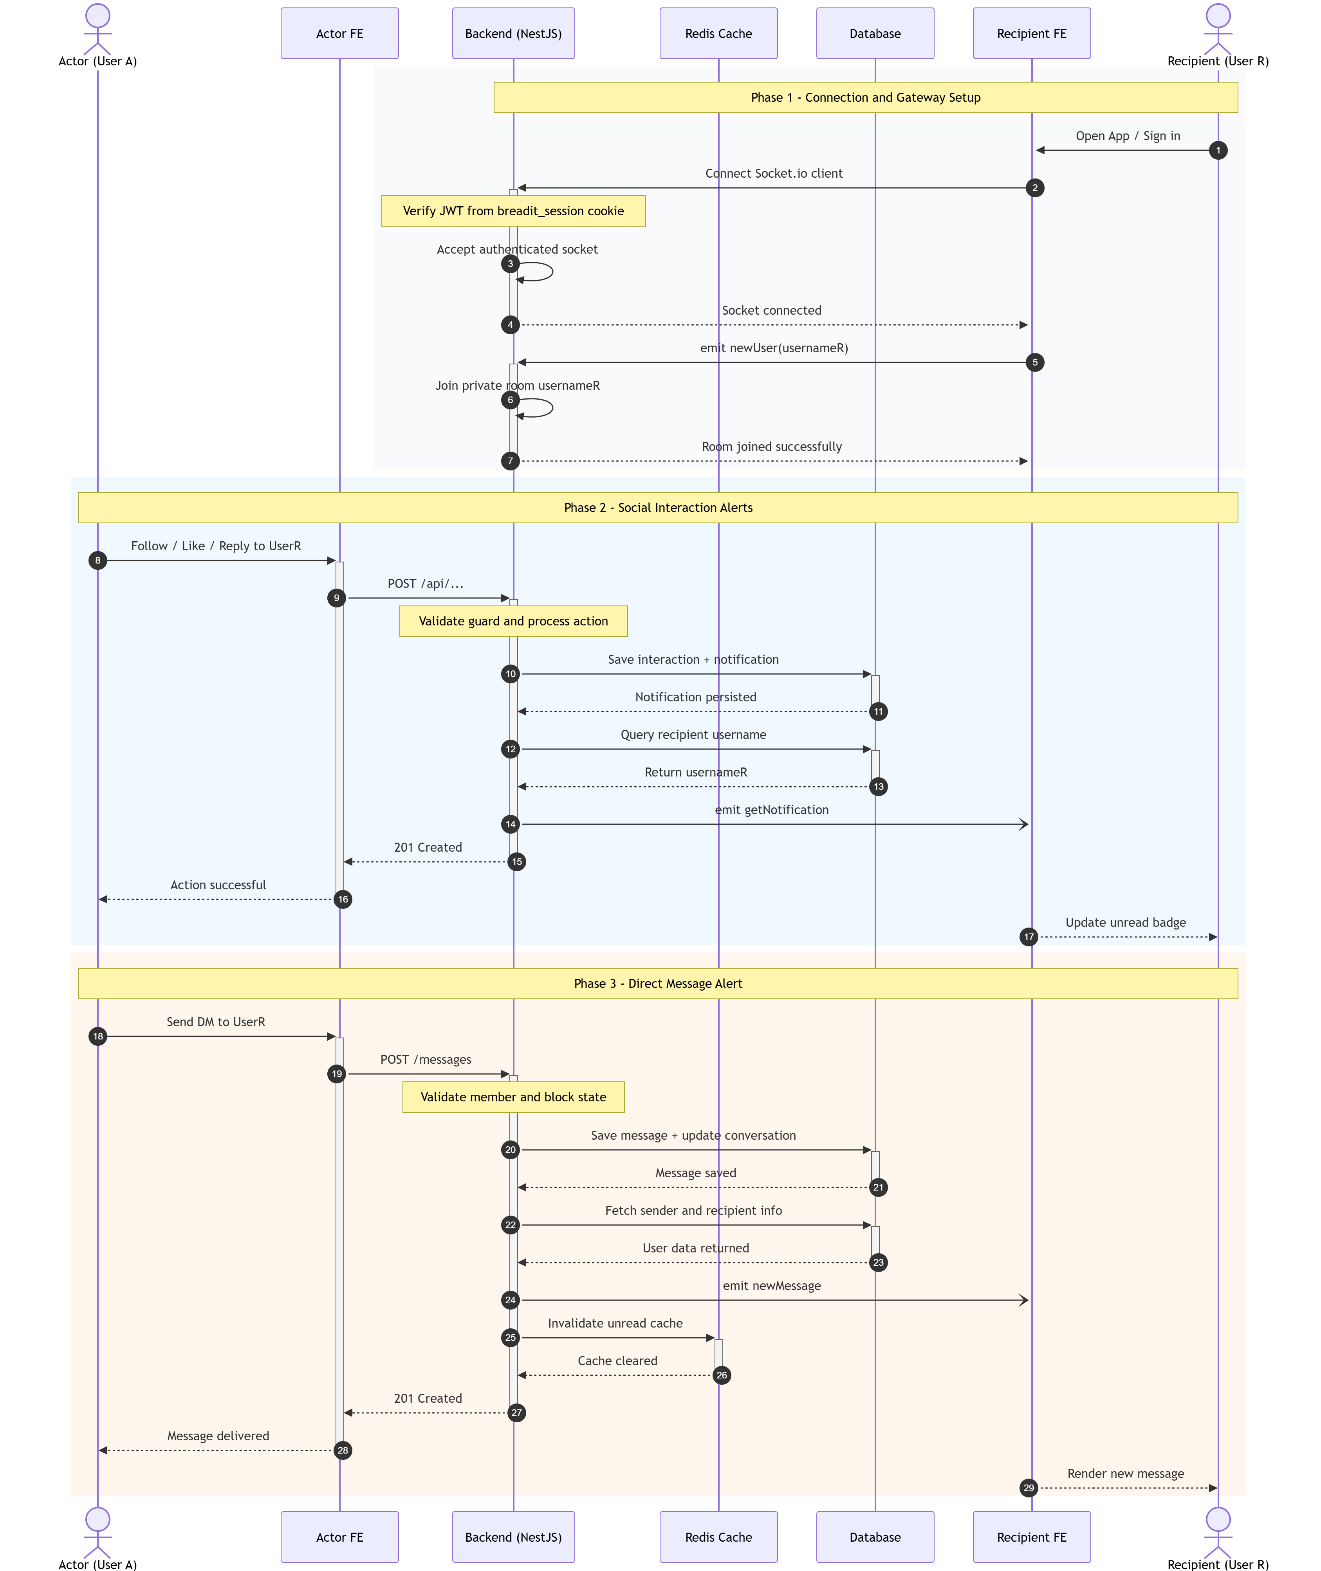
\includegraphics[width=0.92\linewidth,height=0.82\textheight,keepaspectratio]{images/image32.png}
  \caption{Real-time Notifications Diagram}
  \label{fig:27}
\end{figure}

\medskip\noindent\textbf{Community Management}\\[2pt]
\begin{figure}[H]
  \centering
  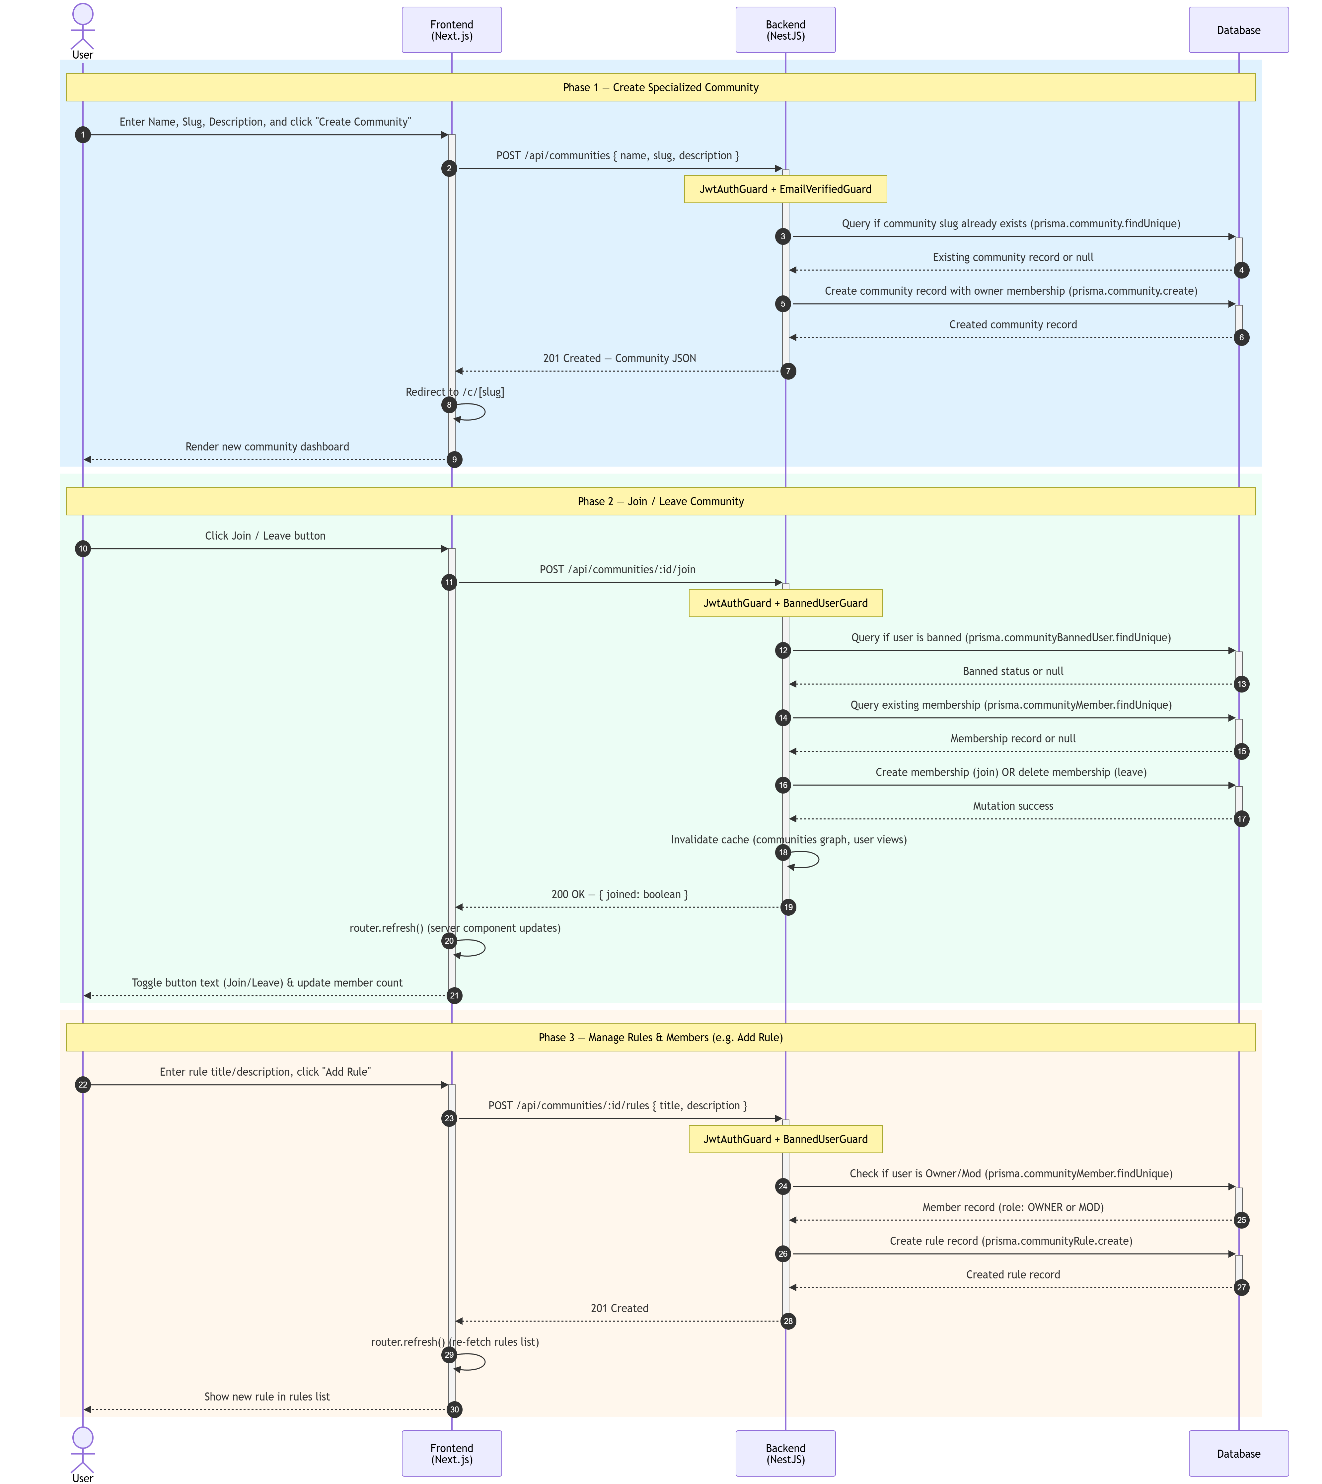
\includegraphics[width=0.92\linewidth,height=0.82\textheight,keepaspectratio]{images/image33.png}
  \caption{Community Management Diagram}
  \label{fig:28}
\end{figure}

\medskip\noindent\textbf{Administrative Moderation}\\[2pt]
\begin{figure}[H]
  \centering
  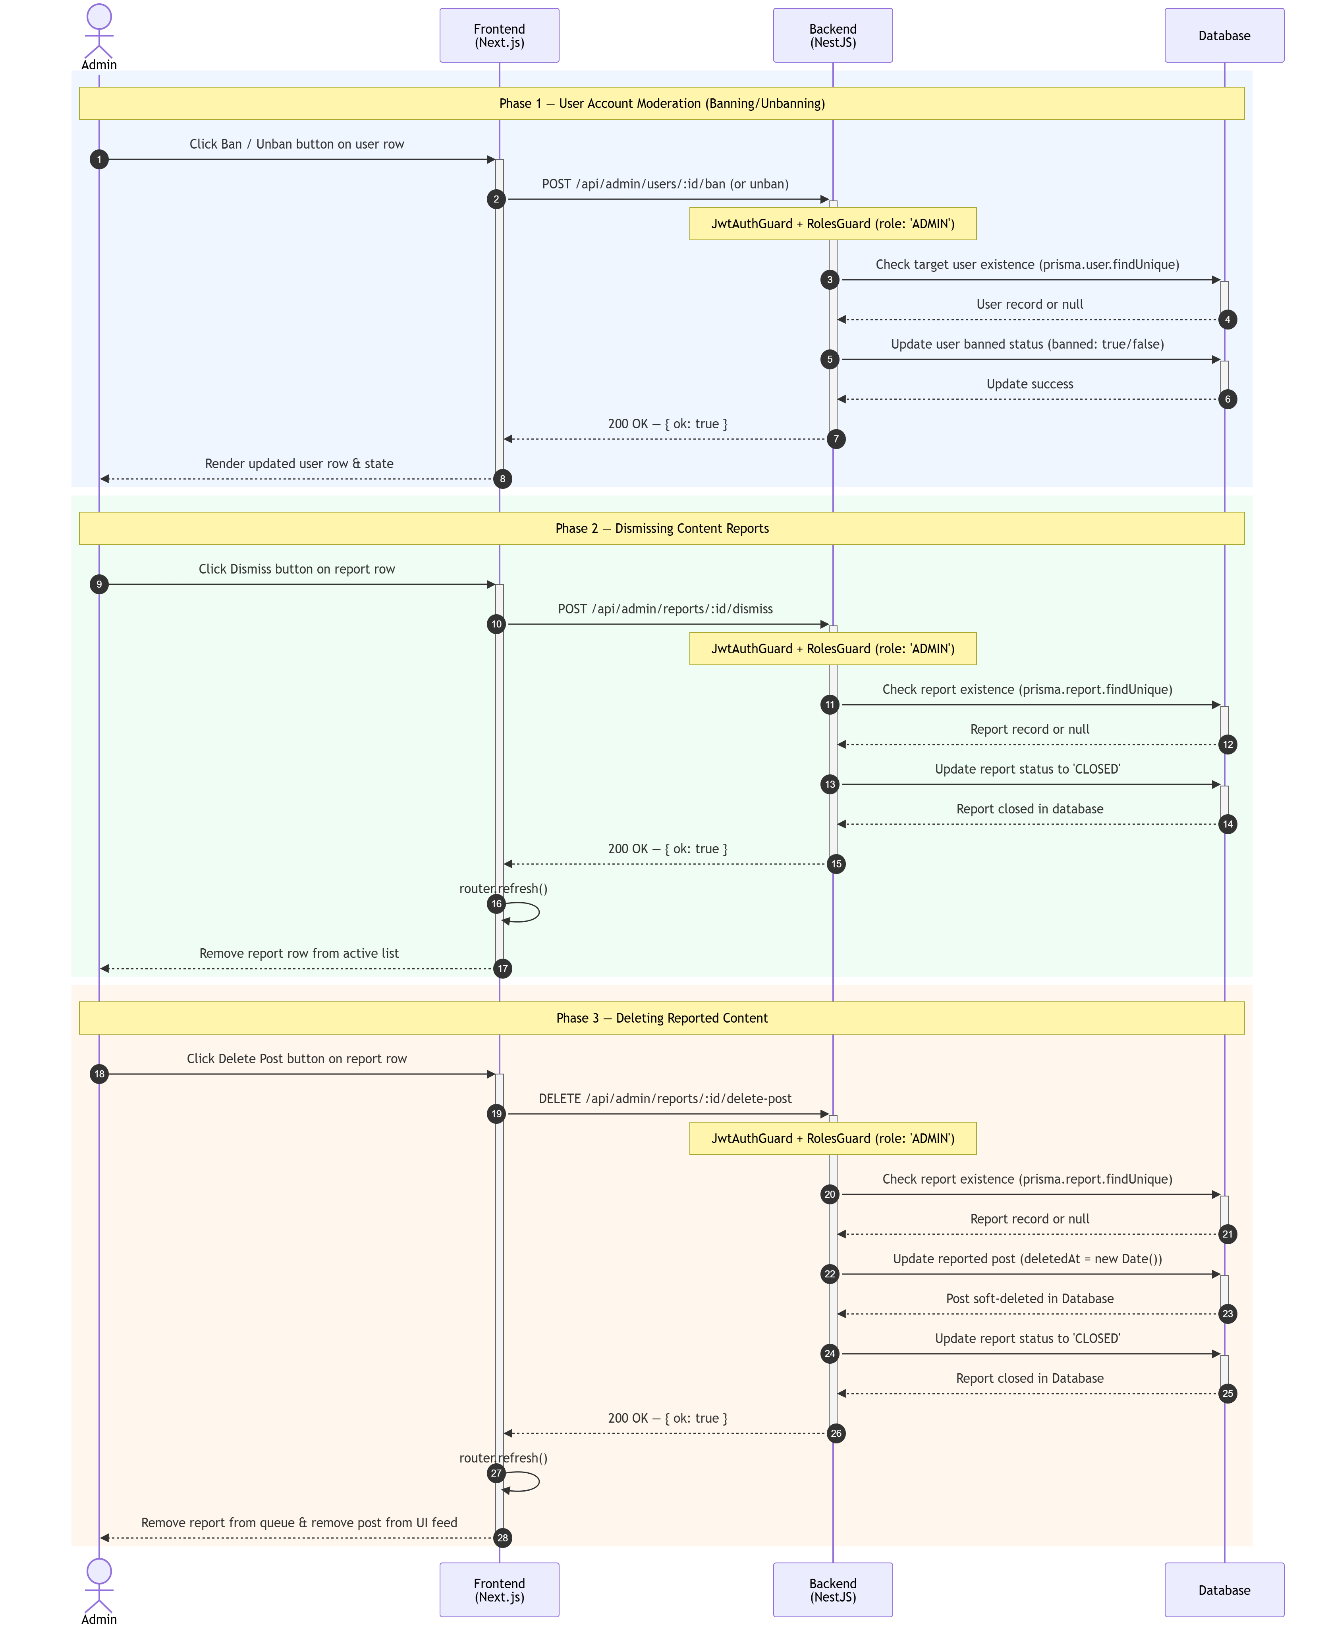
\includegraphics[width=0.92\linewidth,height=0.82\textheight,keepaspectratio]{images/image34.png}
  \caption{Administrative Moderation Diagram}
  \label{fig:29}
\end{figure}

\section{User Requirement Analysis:}

\subsection{User Interface Design:}

Breadit's user interface is split into two primary areas: a public-facing social network and a restricted administrative console. The user interface adapts a standardized three-column grid layout (navigation sidebar, central feed, and contextual discovery widgets) inspired by popular micro-blogging platforms like X/Twitter. This layout maximizes usability and reduces the learning curve for core social interactions. In contrast, the administrative panel uses a dark-themed dashboard focused purely on data visibility and moderation efficiency.

The client-side interface covers the user journey through the following main views:
\begin{itemize}
  \item Authentication \& Verification: Registration (Sign Up), login (Sign In), password recovery, and a 6-digit OTP verification view to validate email ownership.
  \item Unified Feed \& Discovery: Home timeline featuring "For You" (chronological) and "Explore" (trending by likes) tabs, supported by infinite-scroll hashtag feeds and a debounced search dropdown.
  \item Post Details \& Profiles: Individual post views with nested comment threads and media overlays, and user profiles containing filter tabs (Posts, Replies, Media{\ldots}).
  \item Messaging \& Communities: A real-time 1:1 chat interface powered by Socket.IO, and community pages featuring dedicated sub-feeds, group rules, and post submission queues.
  \item 
\end{itemize}

The moderation console contains two core operational views:
\begin{itemize}
  \item User Management (/admin-console/users): A searchable registry of users with controls to ban or reinstate suspended accounts.
  \item Content Moderation (/admin-console/reports): A real-time queue of flagged posts and comments, allowing admins to dismiss reports or delete offending content.
\end{itemize}

To maintain structural clarity and avoid redundant layouts in Chapter 3, mockups and user interface screenshots are excluded from this section and reserved for Chapter 5 (Demonstration). This section concentrates purely on design patterns and architectural user flows. Design inspirations and reference frameworks utilized in formulating the dashboard grid structure are acknowledged in the project bibliography, while screenshots of the deployed application in Chapter 5 document the actual system behavior.

\section{Technology Summary:}

This section provides a detailed overview of the technologies selected for the implementation of the full-stack micro-blogging and real-time social networking platform. While Chapter 2 outlined the theoretical concepts and general characteristics of modern web architectures, this section expands on those fundamentals by specifying their practical applications, architectural roles, and operational integration within the system. The integration of frontend, backend, caching, and database layers forms a cohesive, high-performance stack designed to support fast page rendering, real-time bidirectional communication, and provide an architectural foundation for the future integration of advanced trending and content trending/recommendation algorithms.

\subsection{Front -- end:}

\subsubsection{Technology Used: Next.js}

Next.js 15, powered by React 19, serves as the primary frontend framework for the platform. Utilizing the App Router architecture, Next.js combines Server-Side Rendering (SSR) for static content optimization with client-side interactivity, delivering a highly responsive, performant, and SEO-friendly social media interface.

\subsubsection{Architectural Role}

Next.js is responsible for:
\begin{itemize}
  \item Rendering page layouts and feeds (Home, Explore, Hashtags) dynamically.
  \item Managing user interaction states, including composing posts, liking content, commenting in threads, and updating profile settings.
  \item Communicating the NestJS backend via REST APIs for core CRUD transaction.
  \item Establishing a persistent Socket.IO connection to receive real-time notifications and handle instant messaging.
\end{itemize}

\subsubsection{Key Mechanisms and Features Applied}

\medskip\noindent\textbf{Server \& Client Component Architecture}\\[2pt]

The application leverages the separation of Server and Client components in. Static structures are pre-rendered on the server to optimize loading speeds, while interactive elements are modularized into client-side reusable components, such as:
\begin{itemize}
  \item Layout navigation: Leftbar (menu, user profile link) and Rightbar (search, trending, follow suggestion).
  \item Social interaction: Post (post/reposts), Comment (nested replies) and chat popups.
\end{itemize}

\medskip\noindent\textbf{State Management and Caching (TanStack Query)}\\[2pt]

To manage server state efficiently without complex global store boilerplate:
\begin{itemize}
  \item Instantly reflects actions (toggling a posts like status or following a user) in the UI before the backend confirmation completes, ensuring a zero-latency user experience.
  \item Caches user timelines, notification histories, and search results to prevent redundant API calls.
\end{itemize}

\medskip\noindent\textbf{Real-Time WebSocket Connection (Socket.IO)}\\[2pt]

For real-time features, the client maintains a persistent WebSocket connection.
\begin{itemize}
  \item Pushes real-time alerts (likes, follows, mentions, reposts) to users.
  \item Supports live, bidirectional transmission in the 1:1 chat interface, bypassing the overhead of traditional HTTP polling.
\end{itemize}

\medskip\noindent\textbf{Infinite Scrolling \& Asynchronous Fetching}\\[2pt]

To display long timelines without degrading browser performance, the application implements cursor-based pagination and infinite scrolling. As the next-page items are requested asynchronously, while skeleton screens are shown during data loading states.

\subsubsection{Justification}
\begin{itemize}
  \item Optimized Performance: Built-in features like route pre-fetching and asset optimization drastically reduce initial page load times.
  \item Architectural Flexibility: The modular, hook-driven architecture allows for easy expansion, making the codebase ready to integrate advanced content recommendation systems and trending pipelines in future phase.
\end{itemize}

\subsection{Back -- end:}

\subsubsection{Technology Used: NestJS (TypeScript) + Fastify}

NestJS, running on TypeScript and configured with Fastify as the underlying HTTP server adapter, serves as the main backend framework for the system. This combination provides a modular, highly scalable, and enterprise-grade architecture capable of handling intensive social media and real-time I/O workloads with high concurrency and low latency.

\subsubsection{Architectural Role}

The backend acts as the system's central business logic and data distribution layer:
\begin{itemize}
  \item Handles user session state and authentication (JWT cookie-based authentication)
  \item Manages core social networking domain workflows (feed query generation{\ldots})
  \item Manages database transaction and query logic PostgreSQL via Prisma ORM client.
  \item Dispatches real-time events (likes,notifications,messages) using Socket.IO gateways.
  \item Restricts API access via Guards, Pipes, and Throttling middleware.
\end{itemize}

\subsubsection{Key Mechanisms and Features Applied}

\medskip\noindent\textbf{High-Performance Asynchronous I/O (NestJS + Fastify)}\\[2pt]

Instead of standard Express engines, NestJS is configured with Fastify to support rapid asynchronous I/O execution. This enables:
\begin{itemize}
  \item Fast handling of simultaneous HTTP requests under high traffic.
  \item Efficient processing of pagination queries for massive feeds.
  \item Low-overhead file streaming and media uploads (Fastify's multipart performance).
\end{itemize}

\medskip\noindent\textbf{DTO-Based Data Validation (Class Validator \& Pipes)}\\[2pt]

All incoming API requests go through NestJS ValidationPipes:
\begin{itemize}
  \item Utilizes class-validator and class-transformer to enforce strict DTO (data transfer object) schemas.
  \item Sanitizes input and rejects malformed payloads before they reach service methods, preventing injection attacks and ensuring data integrity.
\end{itemize}

\medskip\noindent\textbf{Modular Architecture \& REST Services}\\[2pt]

The backend is divided into specialized modules (Auth, Users, Posts, Messages, Notifications, Communities) adhering to NestJS's dependency injection principles:
\begin{itemize}
  \item Exposes structured RESTful endpoints (POST /api/auth/register, GET /api/posts/feed
  \item Separates database operations using Prisma client services.
  \item This design supports future migration into isolated microservices if necessary.
\end{itemize}

\medskip\noindent\textbf{Integration with the Trendng/Recommendation Engine}\\[2pt]

\medskip\noindent\textbf{Real-time Event Broadcasting (Socket.IO + Redis Adapter)}\\[2pt]

To support instant notifications and direct messages, the backend implements:
\begin{itemize}
  \item WebSocket Gateways: Encapsulated within Socket.IO gateways to manage client WebSocket sessions.
  \item Redis Adapter: Utilizes redis-adapter to synchronize WebSocket events across multiple server instances, ensuring horizontal scaling.
\end{itemize}

\subsubsection{Justification}

NestJS + Fastify was chosen due to:
\begin{itemize}
  \item Modular and Scalable Structure: Dependency injection and module design result in a highly testable and maintainable codebase.
  \item Substantial Performance Gains: Fastify handles up to two times more requests per second compared to Express, offering optimal resource utilization.
  \item Robust Database Integration: Prisma ORM provides type-safe query building, auto-generated migrations, and high developer velocity.
  \item Ready for Future Scale: The architectural decoupling of services and the integration of Redis adapters ensure the system can scale both vertically and horizontally, easily accommodating real-time recommendation engines or dedicated feed-processing workers in future iterations.
\end{itemize}

\subsection{Database:}

The system incorporates a hybrid storage architecture combining a relational database with an in-memory data store to optimize transactional consistency, real-time state synchronization, and low-latency cache queries.

\subsubsection{Relational Database: PostgreSQL}

\medskip\noindent\textbf{Architectural Role}\\[2pt]

PostgreSQL-the primary relational database, stores all structured application entities:
\begin{itemize}
  \item User Identity \& Relations: Accounts, profile data, bidirectional follow/block relationships.
  \item Content \& Interactions: Posts, media attachments, nested comments, likes, saves, and report logs.
  \item Messaging \& Communities: 1:1 direct messages, conversation memberships, and community settings (rules, bans).
\end{itemize}

\medskip\noindent\textbf{Why PostgreSQL}\\[2pt]
\begin{itemize}
  \item Strong ACID Compliance: Guarantees transaction reliability for user registrations, authentication flows, and content states.
  \item Advanced Relational Modeling: Supports complex self-referencing structures essential for nested comments and reposts.
  \item Seamless ORM Compatibility: Integrates cleanly with Prisma ORM for automated schema migrations and type-safe database queries.
\end{itemize}

\medskip\noindent\textbf{Applied Features}\\[2pt]
\begin{itemize}
  \item Data Integrity Constraints: Unique constraints on fields and compound keys for relationship records.
  \item Query Optimization: Custom indexes on frequently queried fields to speed up timeline rendering.
  \item Atomic Transactions: Atomic database writes via Prisma Transaction APIs to register multiple related records simultaneously.
\end{itemize}

\subsection{Deployment}

The Breadit system is designed to be deployed in a cloud environment using the PaaS (Platform as a Service) and Serverless models. Specialized cloud services help minimize infrastructure management overhead, automate the CI/CD (Continuous Integration/Continuous Deployment) pipeline, and optimize performance for each application component.

The physical deployment architecture consists of the following components:
\begin{itemize}
  \item Frontend (Next.js): Deployed on Vercel (Serverless \& CDN).
  \item Backend (NestJS): Deployed on Render (Containerized Web Service).
  \item Database (PostgreSQL): Manage database service provided by Supabase.
  \item Cache (Redis): The Serverless Redis service provided by Upstash.
  \item Media Storage \& CDN: The cloud storage and media delivery services of Cloudinary.
\end{itemize}

\subsubsection{Workflow}
\begin{center}
  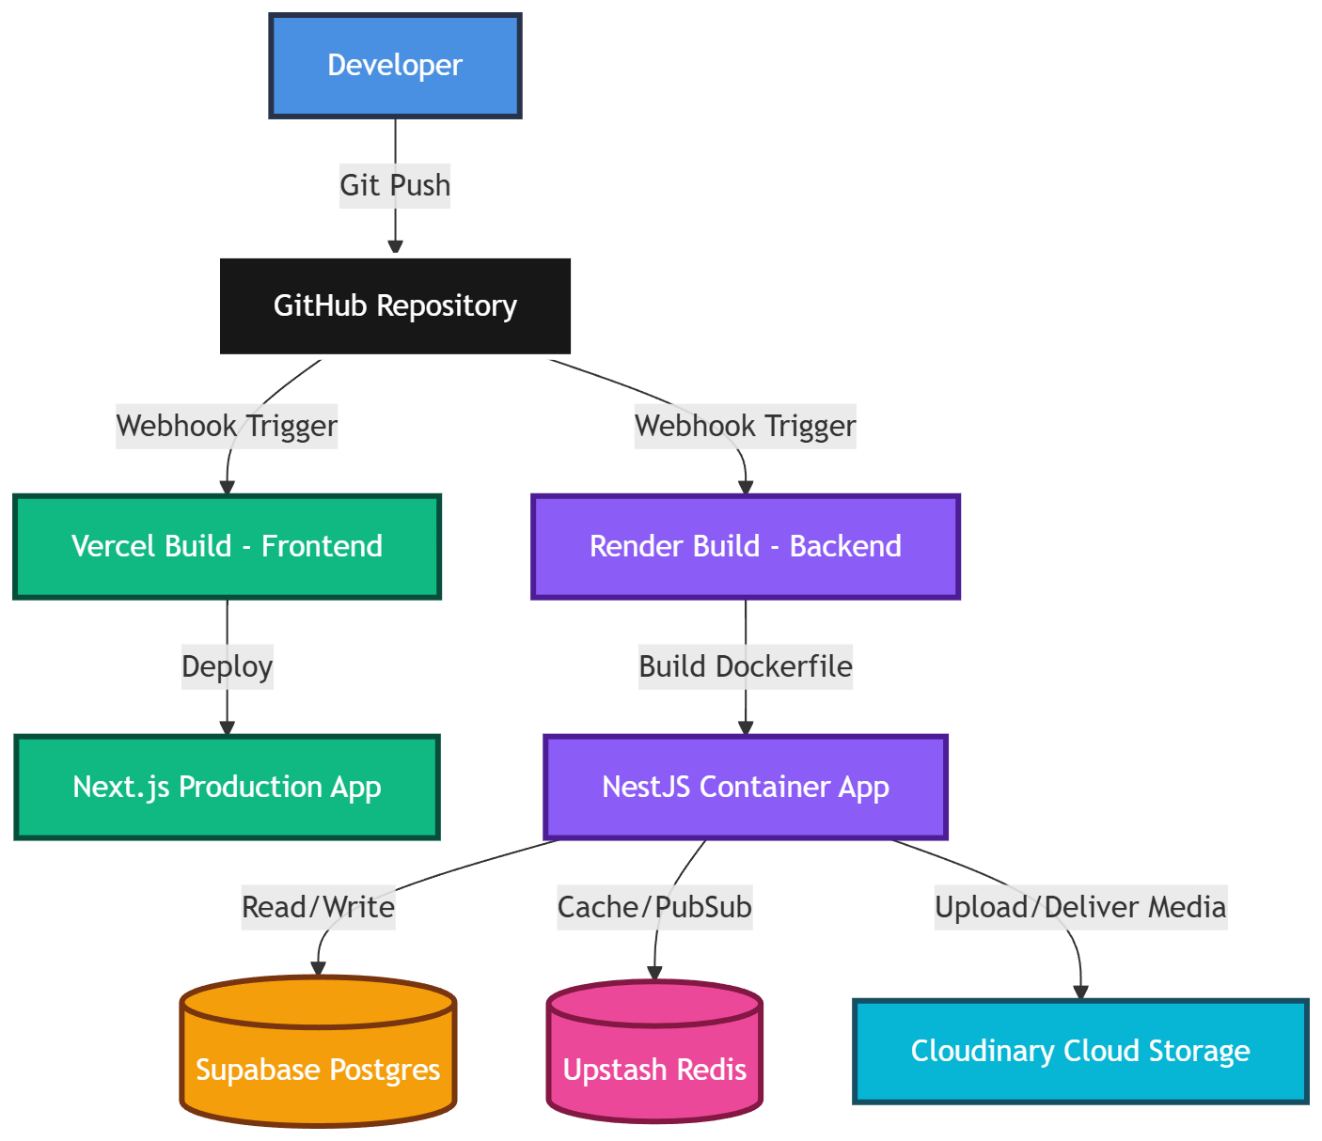
\includegraphics[width=0.92\linewidth,height=0.82\textheight,keepaspectratio]{images/image35.png}
\end{center}

\medskip\noindent\textbf{Flow A: (Frontend)}\\[2pt]
\begin{itemize}
  \item Trigger: The developer pushes new source code to the main branch of the GitHub repository.
  \item Build Pipeline: Vercel detects modifications within the frontend directory (apps/frontend/). An automated build pipeline is triggered on Vercel's infrastructure:
\begin{itemize}
  \item Node.js environment initialization.
  \item Compiling Next.js source code to a production-ready build (optimizing static pages, server-side routes, and minifying assets).
\end{itemize}
  \item Deployment: Once compilation succeeds, the build artifact is deployed and distributed across Vercel's global Edge CDN network. Vercel's router seamlessly redirects user traffic to the new version without any downtime.
\end{itemize}

\medskip\noindent\textbf{Flow B: (Backend)}\\[2pt]
\begin{itemize}
  \item Trigger: Similarly, a push event to the main branch fires a webhook targeting Render.
  \item Docker Build: Render identifies changes in the backend directory (apps/backend/) and reads the configured Dockerfile (apps/backend/Dockerfile):
\begin{itemize}
  \item A multi-stage Docker build runs to minimize the final container image size.
  \item Environment variables such as DATABASE\_URL (pointing to Supabase) and REDIS\_URL (pointing to Upstash) are injected during runtime.
\end{itemize}
  \item Deploy Container: Render spawns the NestJS backend container from the compiled Docker image. It performs continuous health checking via the /api/health endpoint. Once the container responds with a healthy status (200 OK), Render routes incoming API traffic to the new container and safely terminates the deprecated instance.
\end{itemize}

\subsubsection{Networking and Security}
\begin{itemize}
  \item Transport Layer Security (HTTPS/WSS): All connections from user browsers to the Frontend (Vercel) and Backend (Render) are strictly encrypted using HTTPS and WSS (Secure WebSockets). SSL/TLS certificates are provisioned and auto-renewed Encrypt.
  \item CORS (Cross-Origin Resource Sharing): The NestJS backend enforces a strict CORS policy, authorizing only requests originating from the official Frontend domain access API resources.
  \item Database Isolation: PostgreSQL on Supabase and Redis on Upstash are secured behind complex password authentication mechanisms and require SSL-encrypted connections. Database access ports are tightly restricted and shielded from the public internet.
  \item Authentication Security: JWT authentication tokens are securely transmitted between client and server via Cookies configured with the httpOnly flag (mitigating XSS token theft risks) and the Secure flag (restricting transmissions to HTTPS connections only).
\end{itemize}

\subsubsection{Compute and Scalability}
\begin{itemize}
  \item Frontend Compute: Leveraging Vercel's serverless infrastructure, static assets are cached at Edge nodes. Serverless API functions scale up and down instantly to accommodate fluctuating user traffic without manual configuration.
  \item Backend Compute: The NestJS container instance running on Render is continuously monitored for CPU and memory utilization. Under high load, Render supports both vertical scaling (allocating more CPU/RAM resources) and horizontal scaling (replicating multiple container instances running in parallel).
  \item Caching \& Load Reduction: The integration of Upstash Redis allows heavy queries (such as the Trending Feed) to be cached. This significantly alleviates processing overhead on the NestJS backend CPU and reduces direct read IOPS on the primary PostgreSQL database.
\end{itemize}

\subsubsection{Database Service}
\begin{itemize}
  \item The primary data layer of Breadit is powered by Supabase (Managed PostgreSQL):
\begin{itemize}
  \item Database Engine: PostgreSQL 16 running on optimized cloud infrastructure.
  \item Role: Stores structured data across the system, including User Profiles, Posts, Comments, Communities (Sub-breadits), Votes, and Moderation Reports.
  \item Automated Management: Features automated daily backups and Connection Pooling (via PgBouncer/Supabase Pooler) to sustain thousands of concurrent connections from the Backend without exhausting system resources.
  \item ORM Integration: Integrates seamlessly with Prisma ORM on the backend to synchronize schema definitions and execute database migrations safely.
\end{itemize}
\end{itemize}


\chapter{IMPLEMENTATION}

\section{Project Structure Overview:}

The Breadit project is structured as a monorepo utilizing npm workspaces. This architecture decouples the frontend client interface, backend server logic, and shared utility definitions, allowing independent component lifecycle management, easier deployment containerization, and unified types across the platform.
\begin{figure}[H]
  \centering
  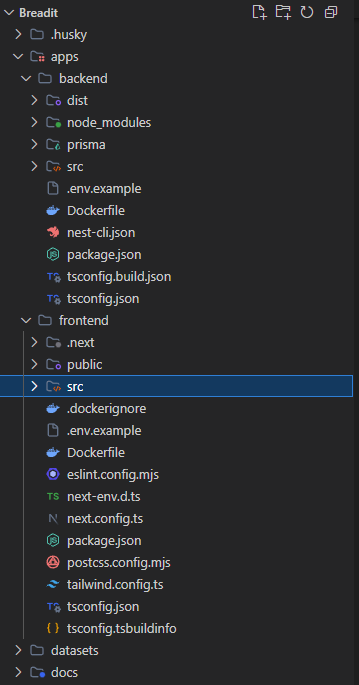
\includegraphics[width=0.92\linewidth,height=0.82\textheight,keepaspectratio]{images/image36.png}
  \caption{Project Structure}
  \label{fig:30}
\end{figure}

\section{Backend Implementation}

The backend functionality of Breadit is developed using the NestJS framework built on top of Fastify for high-performance HTTP request handling and WebSocket communication. The server interacts with a PostgreSQL database using Prisma ORM to manage data persistence and type safety across database operations.

\subsection{Database Models}

The system's data layer architecture is centrally defined in the schema.prisma file. This configuration file houses declarative schema models that Prisma translates into relational database tables and TypeScript interfaces.
\begin{figure}[H]
  \centering
  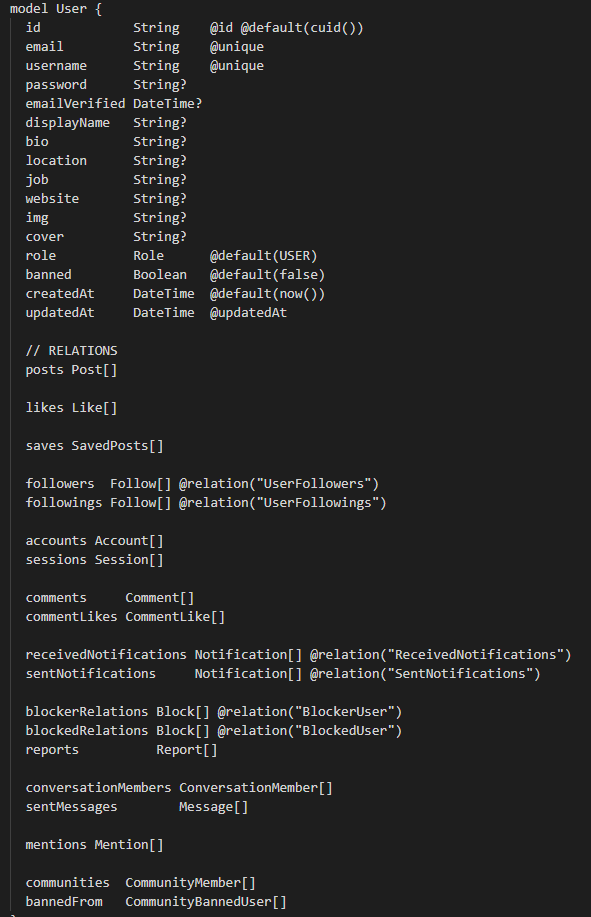
\includegraphics[width=0.92\linewidth,height=0.82\textheight,keepaspectratio]{images/image37.png}
  \caption{Code Snippet -- SiteUser Model Definition}
  \label{fig:31}
\end{figure}

\subsection{Module 1: Authentication \& Account Verification}

\textbf{Controller }\textbf{(API}\textbf{ }\textbf{routes)}\textbf{:} Exposes RESTful endpoints for authentication. It integrates NestJS @Throttle decorators to enforce rate-limiting rules (maximum of 10 requests per 60 seconds) at the entry layer, protecting sensitive operations like Registration, Login, and OTP Verification from automated dictionaries and brute-force attacks.
\begin{figure}[H]
  \centering
  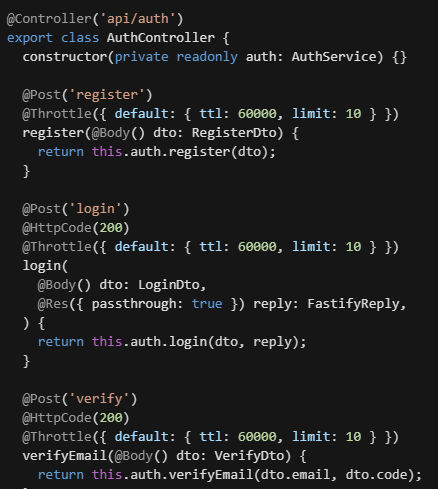
\includegraphics[width=0.92\linewidth,height=0.82\textheight,keepaspectratio]{images/image38.png}
  \caption{Code Snippet -- Authentication \& Account Verification}
  \label{fig:32}
\end{figure}

\textbf{Service (Business Logic)}: Implements secure password verification using bcrypt.compare against hashed credentials stored in PostgreSQL. Upon successful authentication, it generates stateless JSON Web Token (JWT) using the jose library containing the user session claims. This JWT is appended to the Fastify response header via a secure, httpOnly, sameSite: 'lax' cookie, shielding the application from Cross-Site Scripting (XSS) token interception.
\begin{figure}[H]
  \centering
  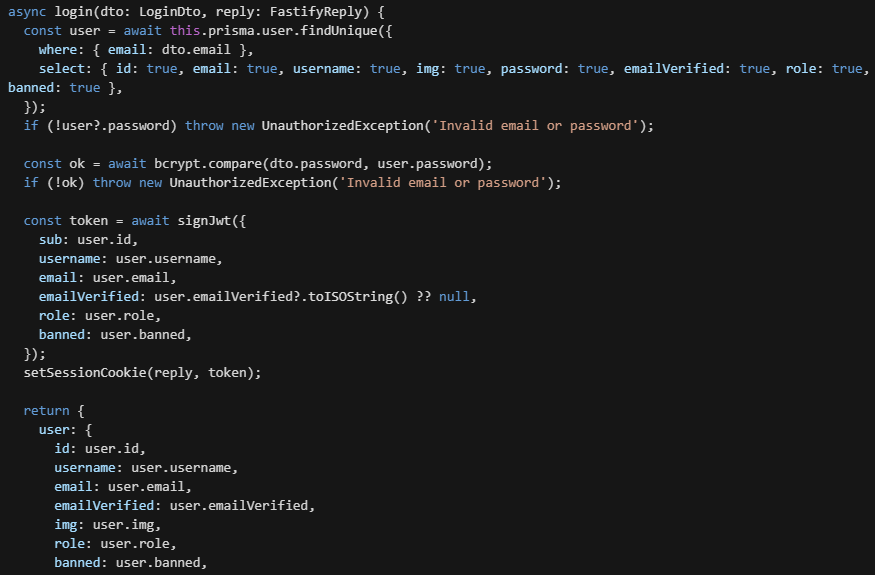
\includegraphics[width=0.92\linewidth,height=0.82\textheight,keepaspectratio]{images/image39.png}
  \caption{Code Snippet -- Authentication \& Account Verification}
  \label{fig:33}
\end{figure}

\subsection{Module 2: Feeds \& Discovery}

\textbf{Controller (API Routes):} Handlers request for dynamic feed retrieval. It utilizes an OptionalJwtAuthGuard to determine session presence: if the request is authenticated, the client is identified (req.user.id) to fetch personalized interactions (such as like and bookmark statuses); if anonymous, the request bypasses session enforcement to serve generic public feeds.
\begin{figure}[H]
  \centering
  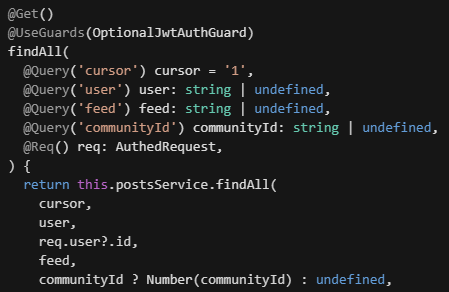
\includegraphics[width=0.92\linewidth,height=0.82\textheight,keepaspectratio]{images/image40.png}
  \caption{Code Snippet -- Feed \& Discovery}
  \label{fig:34}
\end{figure}

\textbf{Service (Business Logic \& Algorithm):} Implements a time-decay explore feed ranking algorithm. The system aggregates dynamic user signals (likes, comments, reposts) and applies a linear decay factor based on post age (ageHours). It further applies a diversity filter (applyExploreDiversity) that limits consecutive posts from the same author to 3, ensuring feed variety and preventing monopoly of the explore feed by single active users.
\begin{figure}[H]
  \centering
  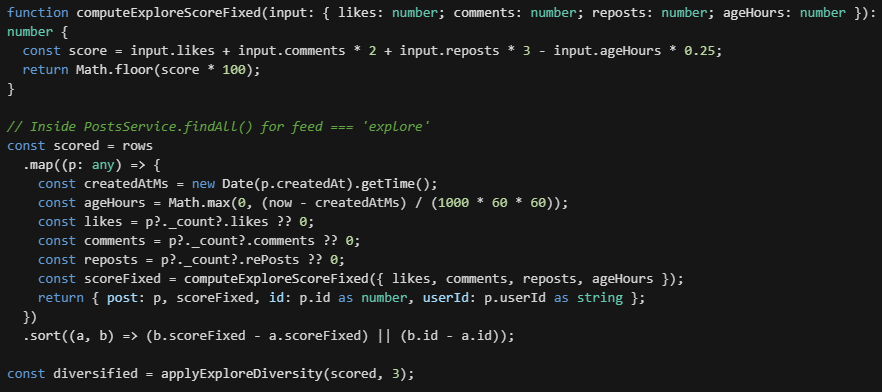
\includegraphics[width=0.92\linewidth,height=0.82\textheight,keepaspectratio]{images/image41.png}
  \caption{Code Snippet -- Feed \& Discovery}
  \label{fig:35}
\end{figure}

\subsection{Module 3: Post Management}

\textbf{Controller (API Routes):} Handles post creation requests submitted via multipart/form-data. Because the project runs on Fastify instead of Express, file uploads are processed asynchronously using non-blocking streams (req.parts()), which significantly reduces memory utilization and avoids high-RAM spikes during concurrent heavy file uploads.
\begin{figure}[H]
  \centering
  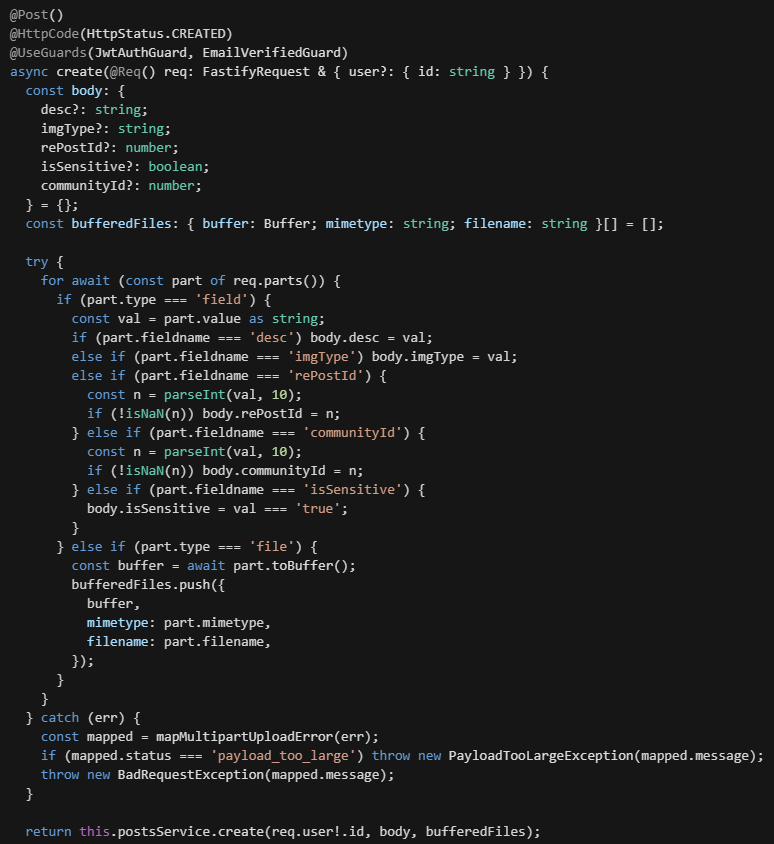
\includegraphics[width=0.92\linewidth,height=0.82\textheight,keepaspectratio]{images/image42.png}
  \caption{Code Snippet -- Post Management}
  \label{fig:36}
\end{figure}

\textbf{Service (Business Logic):} Executes post insertion and handles automatic hashtag discovery. It uses an ES6 RegExp matchAll(/\#([a-zA-Z0-9\_]+)/g) search to isolate tags, eliminate duplicate entries using a Set, and executes concurrent database upsert queries inside a Promise.all block. This establishes hashtag records and many-to-many relationship rows in SQL in a single non-blocking execution block.
\begin{figure}[H]
  \centering
  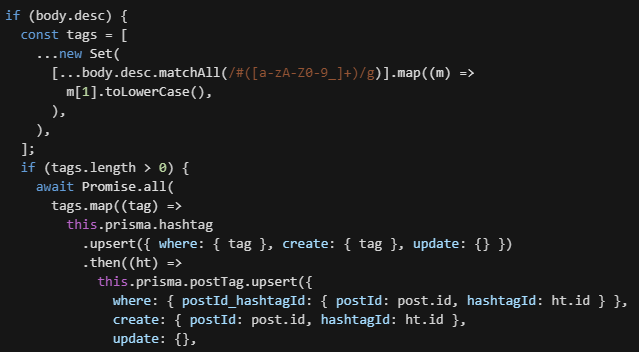
\includegraphics[width=0.92\linewidth,height=0.82\textheight,keepaspectratio]{images/image43.png}
  \caption{Code Snippet -- Post Management}
  \label{fig:37}
\end{figure}

\subsection{Module 4: Post Interaction}

\textbf{Controller (API Routes):} Exposes retrieval routes for comment feeds, integrates NestJS ParseIntPipe to sanitize and cast the parameter postId from a raw string into an integer directly at the controller routing layer, blocking malformed input types before database querying.
\begin{figure}[H]
  \centering
  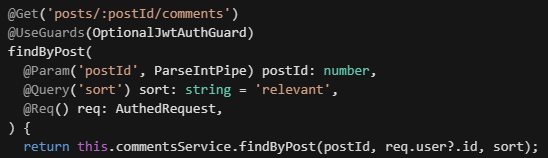
\includegraphics[width=0.92\linewidth,height=0.82\textheight,keepaspectratio]{images/image44.png}
  \caption{Code Snippet -- Post Interaction}
  \label{fig:38}
\end{figure}

\textbf{Service (Business Logic):} Resolves threaded nested hierarchical comment streams. The service executes recursive queries through Prisma, retrieving top-level parent comments and nesting subsequent children (replies) up to 5 levels deep. Root replies are sorted dynamically according to popularity (like count) or recency, while inner child replies are sorted chronologically (createdAt: asc) to maintain coherent thread conversations.
\begin{figure}[H]
  \centering
  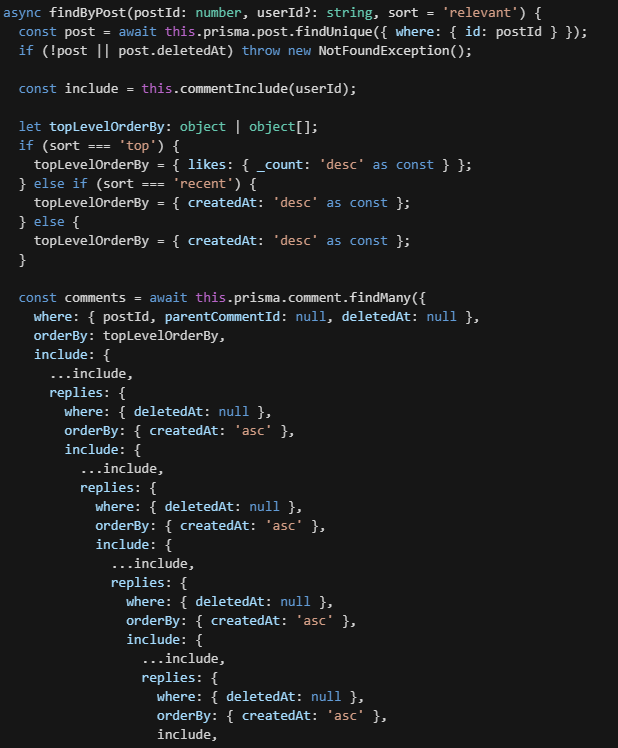
\includegraphics[width=0.92\linewidth,height=0.82\textheight,keepaspectratio]{images/image45.png}
  \caption{Code Snippet -- Post Interaction}
  \label{fig:39}
\end{figure}

\subsection{Module 5: User Relationship Management}

\textbf{Controller (API Routes):} Endpoint that handles user blocks. Combines session validation (JwtAuthGuard) and security moderation checks (BannedUserGuard) to prevent blocked or banned users from initiating relationship modifications on the platform.
\begin{figure}[H]
  \centering
  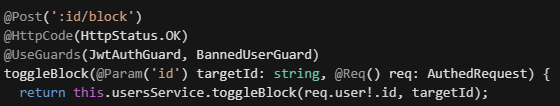
\includegraphics[width=0.92\linewidth,height=0.82\textheight,keepaspectratio]{images/image46.png}
  \caption{Code Snippet -- User Relationship Management}
  \label{fig:40}
\end{figure}

\textbf{Service (Business Logic):} Implements bidirectional blocking logic. When a block is established, the database removes mutual follow instances in a unified transaction (deleteMany). Cache invalidation commands are pushed immediately to Redis to delete old relationship state graphs (graph:follows and graph:blockedPeers), enforcing instant privacy boundaries on subsequent page requests.
\begin{center}
  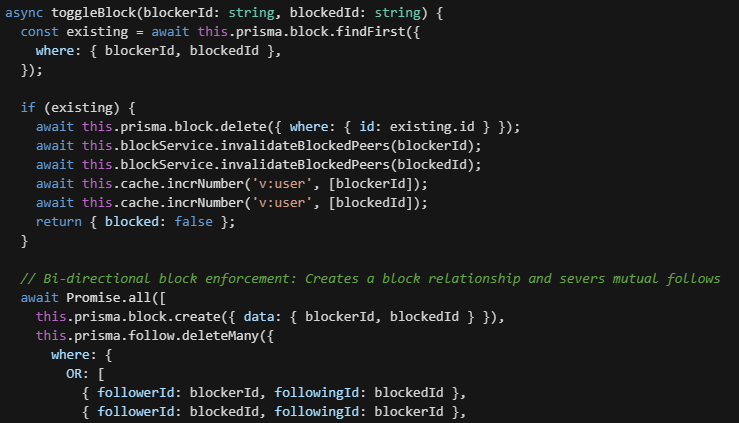
\includegraphics[width=0.92\linewidth,height=0.82\textheight,keepaspectratio]{images/image47.png}
\end{center}
\begin{figure}[H]
  \centering
  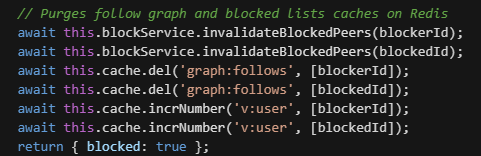
\includegraphics[width=0.92\linewidth,height=0.82\textheight,keepaspectratio]{images/image48.png}
  \caption{Code Snippet -- User Relationship Management}
  \label{fig:41}
\end{figure}

\subsection{Module 6: Profile Management}

\textbf{Controller (API Routes):} Defines routes for loading specific user profiles. Uses the OptionalJwtAuthGuard to verify session parameters, allowing guests to read profiles while letting authenticated users pass search queries (q) and tab queries.
\begin{figure}[H]
  \centering
  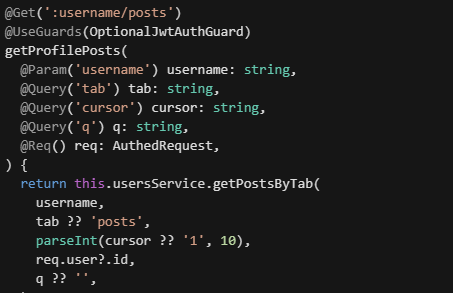
\includegraphics[width=0.92\linewidth,height=0.82\textheight,keepaspectratio]{images/image49.png}
  \caption{Code Snippet -- Profile Management}
  \label{fig:42}
\end{figure}

\textbf{Service (Business Logic):} Dynamically compiles PostgreSQL where conditions are based on selected categories (media, likes, posts). Security checks are enforced inside the service (isBlockedPair) to verify blocking status before compiling profile content, blocking malicious API requests from bypass attempts.
\begin{center}
  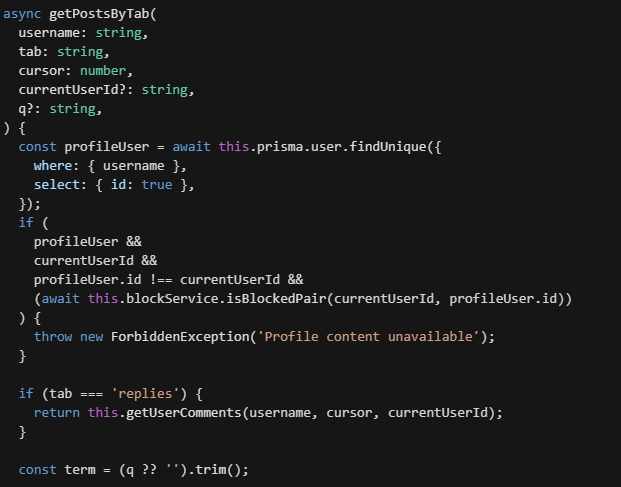
\includegraphics[width=0.92\linewidth,height=0.82\textheight,keepaspectratio]{images/image50.png}
\end{center}
\begin{center}
  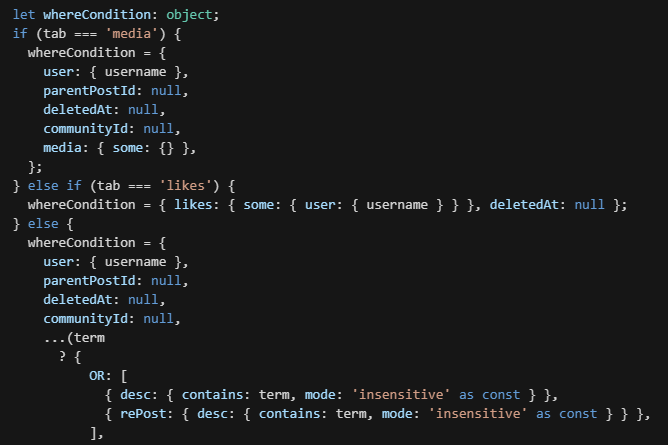
\includegraphics[width=0.92\linewidth,height=0.82\textheight,keepaspectratio]{images/image51.png}
\end{center}
\begin{figure}[H]
  \centering
  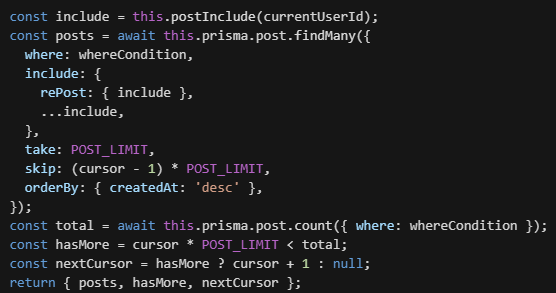
\includegraphics[width=0.92\linewidth,height=0.82\textheight,keepaspectratio]{images/image52.png}
  \caption{Code Snippet -- Profile Management}
  \label{fig:43}
\end{figure}

\subsection{Module 7: Direct Messaging}

\textbf{Controller (API Routes):} Routing endpoint for message dispatching. Guarded by the EmailVerifiedGuard to restrict real-time communication privileges to verified users, preventing malicious spam and automated bot registration flows.
\begin{figure}[H]
  \centering
  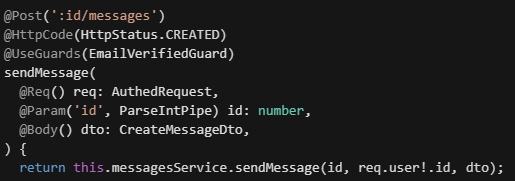
\includegraphics[width=0.92\linewidth,height=0.82\textheight,keepaspectratio]{images/image53.png}
  \caption{Code Snippet -- Direct Messaging}
  \label{fig:44}
\end{figure}

\textbf{Service (Business Logic):} Encapsulates message creation and conversation metadata updates within an ACID \$transaction block. Once changes are successfully written to SQL, the service leverages Socket.io WebSocket Gateway to broadcast the message payload (newMessage event) to the recipient's secure connection channel, subsequently invalidating the unread count in Redis.
\begin{center}
  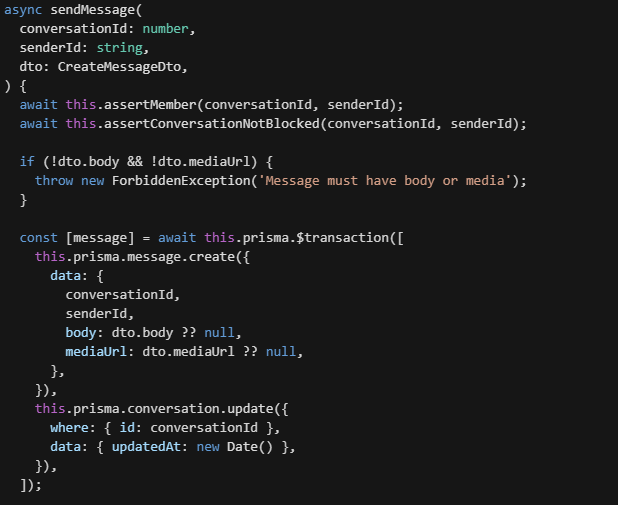
\includegraphics[width=0.92\linewidth,height=0.82\textheight,keepaspectratio]{images/image54.png}
\end{center}
\begin{figure}[H]
  \centering
  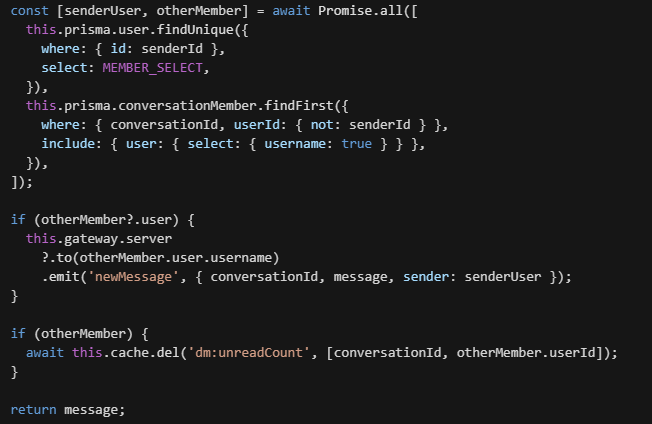
\includegraphics[width=0.92\linewidth,height=0.82\textheight,keepaspectratio]{images/image55.png}
  \caption{Code Snippet -- Direct Messaging}
  \label{fig:45}
\end{figure}

\subsection{Module 8: Real-time Notifications}

\textbf{Controller (API Routes):} Handlers request for reading the authenticated user's notification log history, supporting paging via integer cursors and filters for read/unread notification states.
\begin{figure}[H]
  \centering
  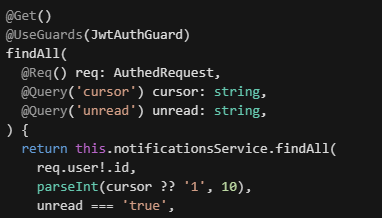
\includegraphics[width=0.92\linewidth,height=0.82\textheight,keepaspectratio]{images/image56.png}
  \caption{Code Snippet -- Real-time Nofications}
  \label{fig:46}
\end{figure}

\textbf{WebSocket Gateway (Real-time Hub):} Implements a full-duplex WebSocket hub powered by Socket.io. It integrates @socket.io/redis-adapter to enable cluster pub/sub synchronization, allowing horizontal scaling of backend instances. It reads the incoming handshake headers to fetch the breadit\_session cookie, validation-checking the JWT signature before establishing the connection.
\begin{figure}[H]
  \centering
  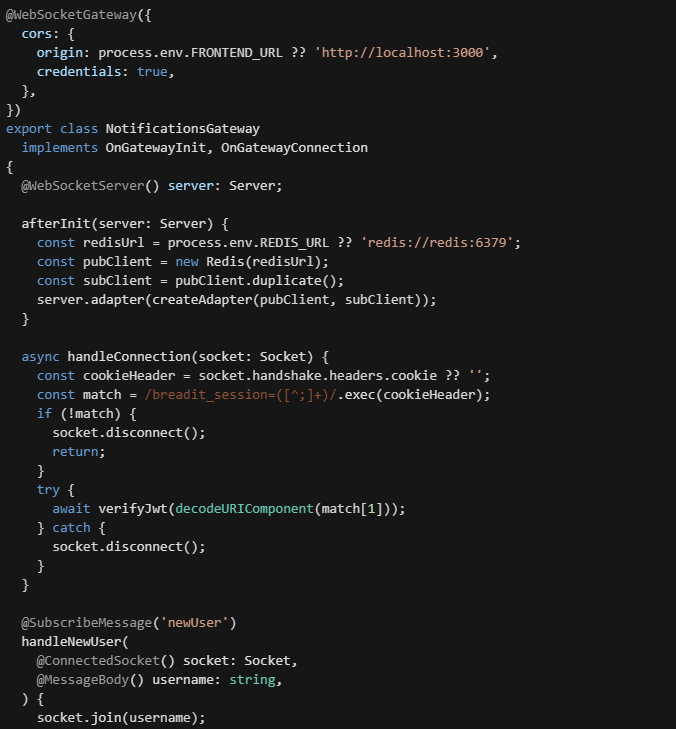
\includegraphics[width=0.92\linewidth,height=0.82\textheight,keepaspectratio]{images/image57.png}
  \caption{Code Snippet -- Real-time Nofications}
  \label{fig:47}
\end{figure}

\subsection{Module 9: Community Management}

\textbf{Controller (API Routes):} Exposes endpoint for community moderators to approve or reject pending member posts, validating basic request parameters (id and postId format) before calling the Service layer.
\begin{figure}[H]
  \centering
  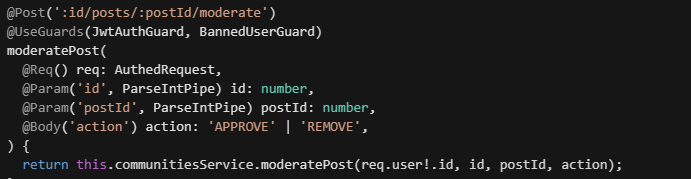
\includegraphics[width=0.92\linewidth,height=0.82\textheight,keepaspectratio]{images/image58.png}
  \caption{Code Snippet -- Community Management}
  \label{fig:48}
\end{figure}

\textbf{Service (Business Logic):} Implements community-level role-based access control (RBAC). The member's moderator/owner status in PostgreSQL before update the target post's isApproved flag. Posts trigger async notifications (COMMUNITY\_NEW\_POST) dispatched concurrently to all community members via Promise.all.
\begin{figure}[H]
  \centering
  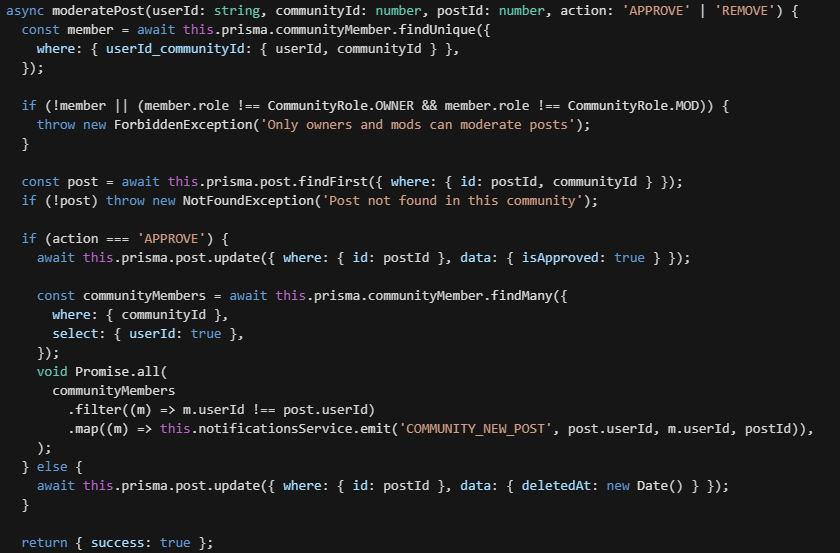
\includegraphics[width=0.92\linewidth,height=0.82\textheight,keepaspectratio]{images/image59.png}
  \caption{Code Snippet -- Community Management}
  \label{fig:49}
\end{figure}

\subsection{Module 10: Administrative Moderation}

\textbf{Controller (API Routes):} Controller endpoint for global moderation. Access is restricted by using global guards (RolesGuard) to verify that the executing account holds a site-wide role of 'ADMIN' before processing bans.
\begin{figure}[H]
  \centering
  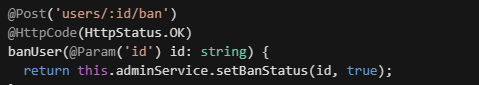
\includegraphics[width=0.92\linewidth,height=0.82\textheight,keepaspectratio]{images/image60.png}
  \caption{Code Snippet -- Administrative Moderation}
  \label{fig:50}
\end{figure}

\textbf{Service (Business Logic}\textbf{)}: Updates a user account's banned state in PostgreSQL. Ensure instant moderation enforcement, the service immediately emits an accountBanned event to the user's active WebSocket room. The client-side application listens for this event to clear session state, revoke cookies, and force redirect the user to prevent the interaction.
\begin{figure}[H]
  \centering
  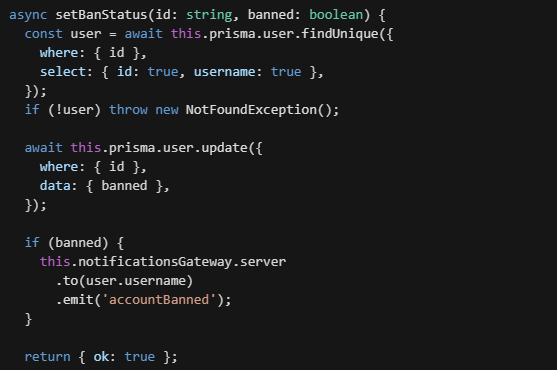
\includegraphics[width=0.92\linewidth,height=0.82\textheight,keepaspectratio]{images/image61.png}
  \caption{Code Snippet -- Administrative Moderation}
  \label{fig:51}
\end{figure}

\section{Frontend Implementation}

The frontend application of Breadit serves as the interactive presentation layer. It is built using the Next.js 15 framework and follows component-based architecture. Client-side state and caching are managed using TanStack React Query, while routing and route guards are handled through Next.js App Router and server-side middleware, ensuring a responsive and seamless user experience.

\subsection{Authentication \& Onboarding Flow (/sign-up, /sign-in, /verify)}
\begin{itemize}
  \item Regex-based Client Validation: During user registration, the system validates the email format instantly in real-time (onChange) utilizing the validateEmail function and a custom regular expression (EMAIL\_RE). This provides instant visual feedback to the user, preventing unnecessary HTTP requests to the backend API.
  \item Stateful Query Parameter Interception: The Login component reads URL query parameters (verified, reset, ban	ned) to dynamically display administrative status alerts (such as informing banned users of account suspension).
  \item OTP Submission Flow: Upon successful registration, the client routes the user to the OTP page. The component enforces a strict 6-digit numeric pattern verification (pattern="[0-9]\{6\}" and inputMode="numeric") before enabling form submission. It invokes the verification API asynchronously and redirects the user to the login screen with a success query parameter upon approval.
\end{itemize}
\begin{figure}[H]
  \centering
  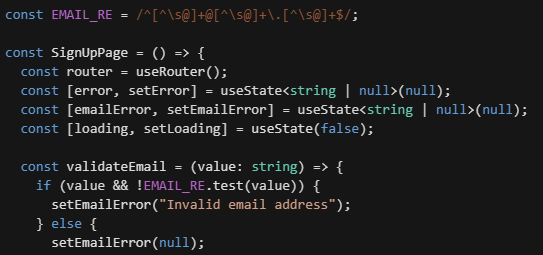
\includegraphics[width=0.92\linewidth,height=0.82\textheight,keepaspectratio]{images/image62.png}
  \caption{Code Snippet -- Sign-Up Page}
  \label{fig:52}
\end{figure}
\begin{figure}[H]
  \centering
  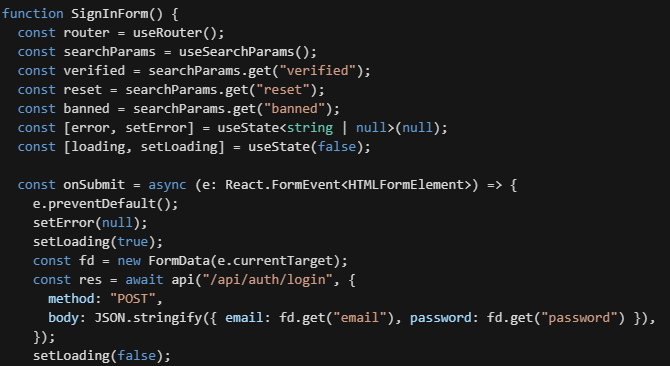
\includegraphics[width=0.92\linewidth,height=0.82\textheight,keepaspectratio]{images/image64.png}
  \caption{Code Snippet -- Sign-In Page}
  \label{fig:53}
\end{figure}
\begin{figure}[H]
  \centering
  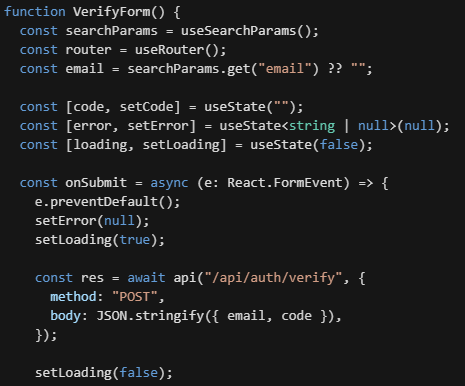
\includegraphics[width=0.92\linewidth,height=0.82\textheight,keepaspectratio]{images/image65.png}
  \caption{Code Snippet -- Verify Page}
  \label{fig:54}
\end{figure}

\subsection{Main Feed \& Discovery Page (/ - Home \& Explore Feed)}
\begin{itemize}
  \item URL-Driven Tabs: The / (Home) route parses the URL search parameters to retrieve the specific active feed type (For you, Explore, Following, Communities). This value is passed down to the Feed wrapper.
  \item useInfiniteQuery Integration: The client-side logic leverages TanStack's useInfiniteQuery hook. By specifying an initial page parameter of 1, the client fetches post items asynchronously. The query key depends on the active tab and filters (userProfileId, feed, communityId), enabling independent cache for each view.
  \item Cursor-based Pagination \& Scroll Trigger: The API returns a nextCursor value. The hook reads this via getNextPageParam to keep track of the subsequent page's cursor. The InfiniteScroll component monitors window scrolls parameters; when the user nears the page bottom, it triggers fetchNextPage, requesting the next page. This forms a smooth, Twitter-like feed scroll experience.
\end{itemize}
\begin{figure}[H]
  \centering
  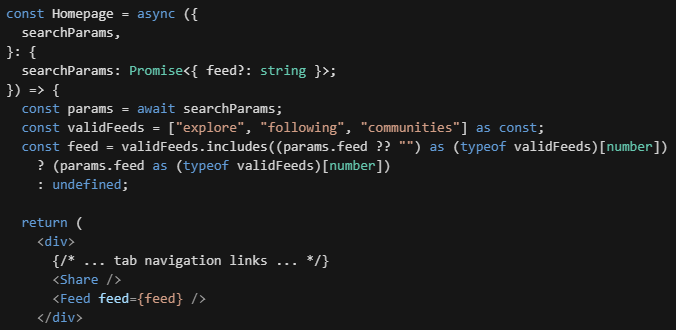
\includegraphics[width=0.92\linewidth,height=0.82\textheight,keepaspectratio]{images/image66.png}
  \caption{Code Snippet -- Feed Routing Layout}
  \label{fig:55}
\end{figure}
\begin{center}
  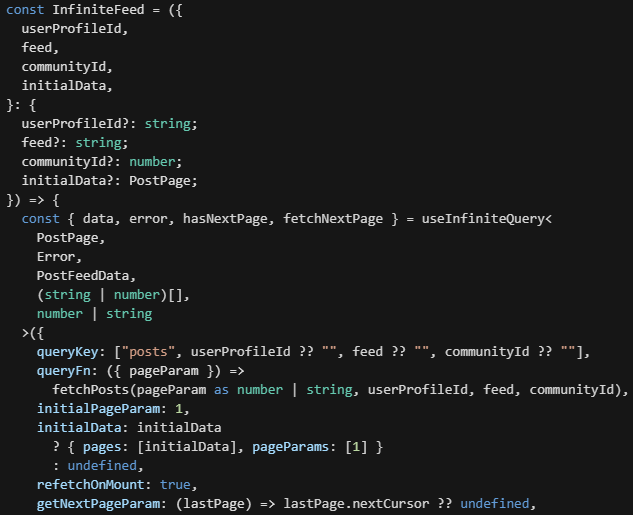
\includegraphics[width=0.92\linewidth,height=0.82\textheight,keepaspectratio]{images/image67.png}
\end{center}
\begin{figure}[H]
  \centering
  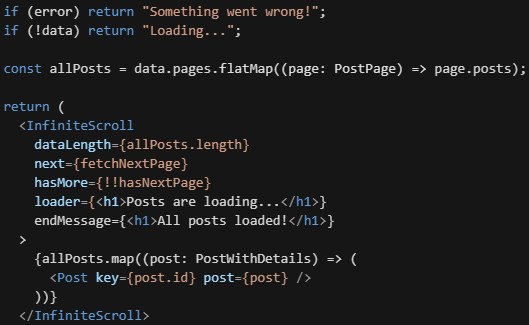
\includegraphics[width=0.92\linewidth,height=0.82\textheight,keepaspectratio]{images/image68.png}
  \caption{Code Snippet -- Main Home Page}
  \label{fig:56}
\end{figure}

\subsection{Direct Messaging \& Chat Interface (/messages)}
\begin{itemize}
  \item WebSocket Handshake and Session Security: The React client establishes a persistent connection with the NestJS Socket.io server, utilizing withCredentials: true to forward session credentials.
  \item Event-Driven Thread Updates: Inside MessageThread.tsx, the component registers event listeners. When the server emits a new message payload, the callback triggers immediately, modifying the TanStack React Query cache dynamically via queryClient.setQueryData to append the message to the view, and performing a smooth programmatic scroll to focus on the new message.
  \item Room-scoped Typing Broadcasts: The custom hook useTypingIndicator manages room-scoped typing indicators. Upon mount, the client joins a conversation room. Typing input textareas trigger onKeystroke(), which emits startTyping events and sets a 3-second debounce timer. If typing stops, stopTyping is emitted. Meanwhile, the client listens to incoming userTyping / userStopTyping events to display real-time feedback.
\end{itemize}
\begin{figure}[H]
  \centering
  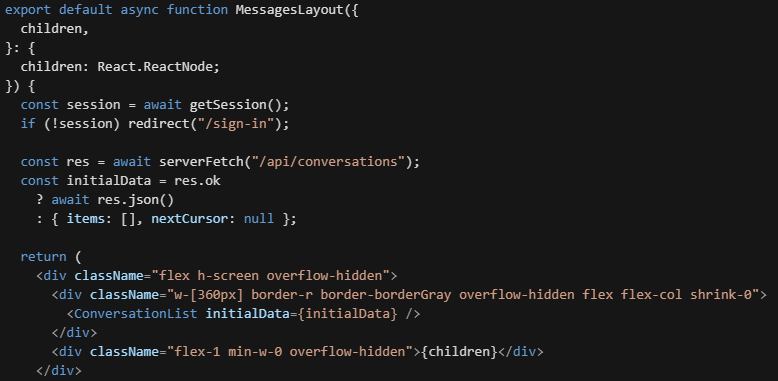
\includegraphics[width=0.92\linewidth,height=0.82\textheight,keepaspectratio]{images/image69.png}
  \caption{Code Snippet -- Messages Layout}
  \label{fig:57}
\end{figure}
\begin{figure}[H]
  \centering
  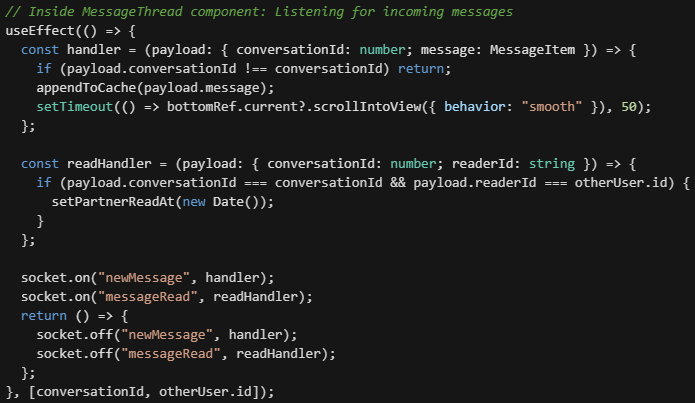
\includegraphics[width=0.92\linewidth,height=0.82\textheight,keepaspectratio]{images/image70.png}
  \caption{Code Snippet -- Real-time Message Thread}
  \label{fig:58}
\end{figure}
\begin{figure}[H]
  \centering
  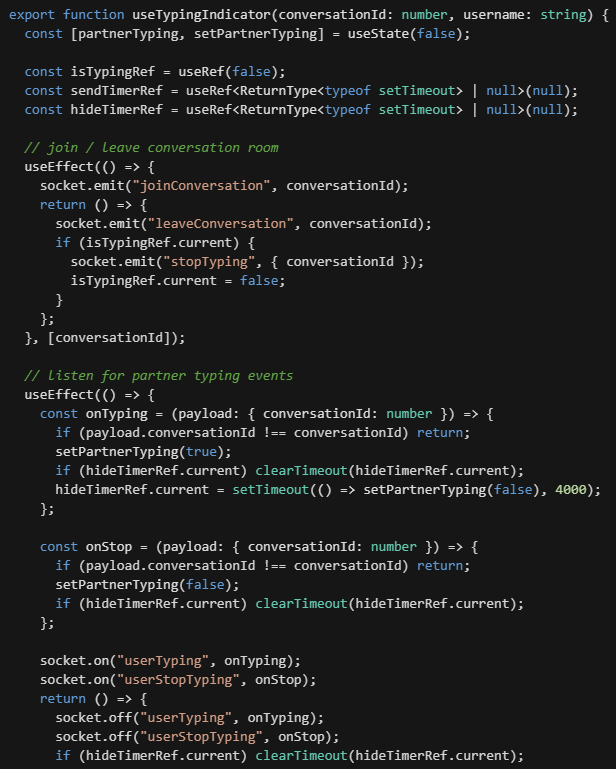
\includegraphics[width=0.92\linewidth,height=0.82\textheight,keepaspectratio]{images/image71.png}
  \caption{Code Snippet -- Typing Indicator Hook}
  \label{fig:59}
\end{figure}

\subsection{User Profile Page (/[username])}
\begin{itemize}
  \item Block-Aware Server Rendering: In [username]/page.tsx, the server performs a pre-fetch on the target user's details. If relationship flags (blockedYou or blockedByYou) are true, the page is flagged as profileRestricted, returning a localized privacy screen instead of sensitive details.
  \item Interactive Tabs: In ProfileTabs.tsx, the client switches between tab selections (posts, replies, media, likes). Updating the activeTab state changes the query key of useInfiniteQuery in ProfileTabFeed.tsx.
  \item Dynamic Query Invalidation: Changing the tab triggers a react-query cache reset and initiates a HTTP request targeting /api/users/\$\{username\}/posts?tab=\$\{activeTab\} with credentials. The component captures 403 Forbidden statuses to prevent restricted users from accessing api-sensitive details.
\end{itemize}
\begin{figure}[H]
  \centering
  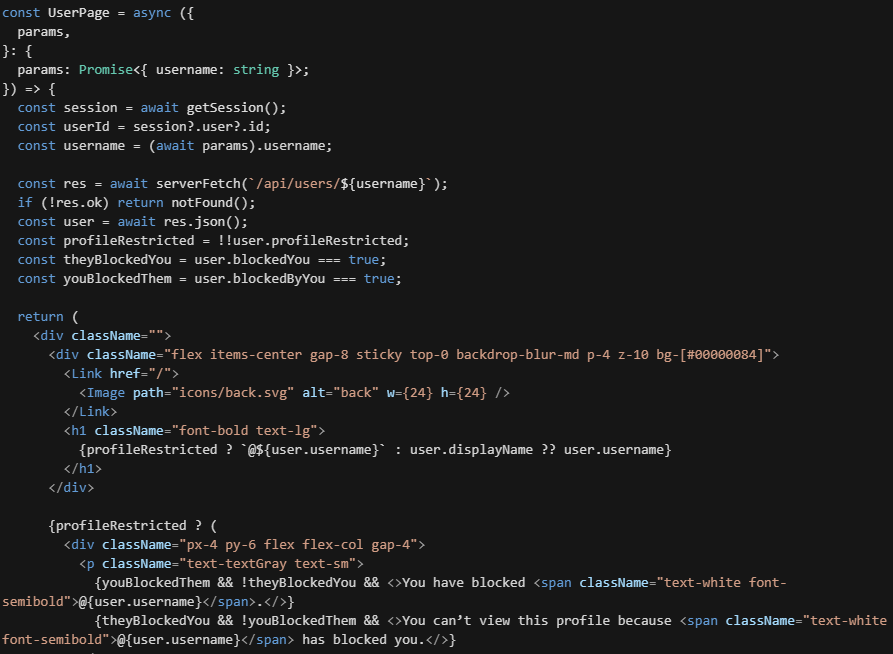
\includegraphics[width=0.92\linewidth,height=0.82\textheight,keepaspectratio]{images/image72.png}
  \caption{Code Snippet -- Server-Side Profile Page}
  \label{fig:60}
\end{figure}
\begin{figure}[H]
  \centering
  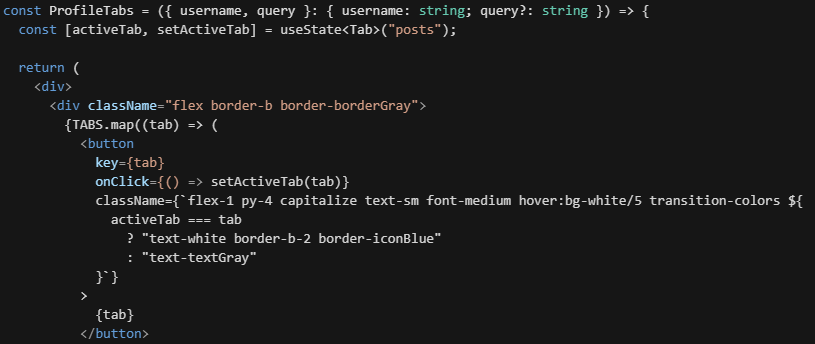
\includegraphics[width=0.92\linewidth,height=0.82\textheight,keepaspectratio]{images/image73.png}
  \caption{Code Snippet -- Profile Tab Switching}
  \label{fig:61}
\end{figure}
\begin{figure}[H]
  \centering
  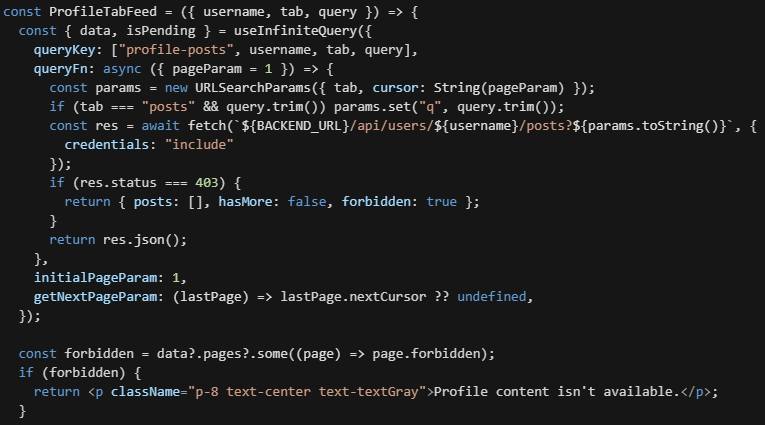
\includegraphics[width=0.92\linewidth,height=0.82\textheight,keepaspectratio]{images/image74.png}
  \caption{Code Snippet -- Profile Feed Fetcher}
  \label{fig:62}
\end{figure}

\subsection{Community Page (/c/[slug])}
\begin{itemize}
  \item Session-Forwarding Server Fetch: Next.js Server Components load the community config (getCommunity) on the server. By parsing cookies using cookies() and forwarding the JWT payload (breadit\_session) in headers, the backend determines membership roles prior to rendering the DOM, preventing unauthorized content leak.
  \item Optimistic State Updates: In CommunityHeader.tsx, the Join/Leave trigger uses a React Query mutation (useMutation). Upon success, it fires router.refresh(), triggering Next.js to re-verify server components and update UI labels dynamically.
  \item Role-Based Pending Queue (Moderator Queue): If the user is flagged as an OWNER or MOD, the page injects the PendingPostsBanner component. This fetch pending community posts from /api/communities/\$\{id\}/posts/pending and exposes instant Approve or Reject buttons. Moderation actions execute asynchronously, filtering out moderated posts instantly from the list.
\end{itemize}
\begin{figure}[H]
  \centering
  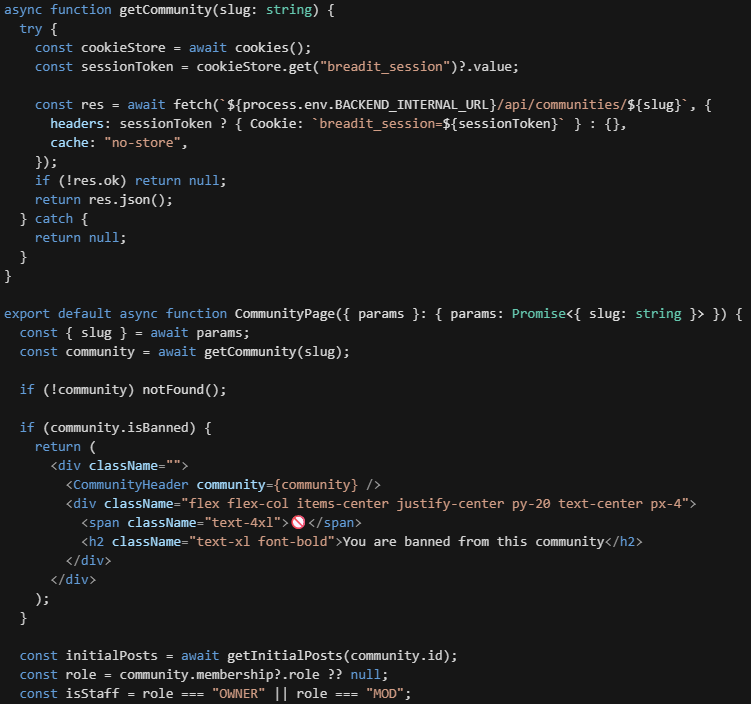
\includegraphics[width=0.92\linewidth,height=0.82\textheight,keepaspectratio]{images/image75.png}
  \caption{Code Snippet -- Community Server Component}
  \label{fig:63}
\end{figure}
\begin{figure}[H]
  \centering
  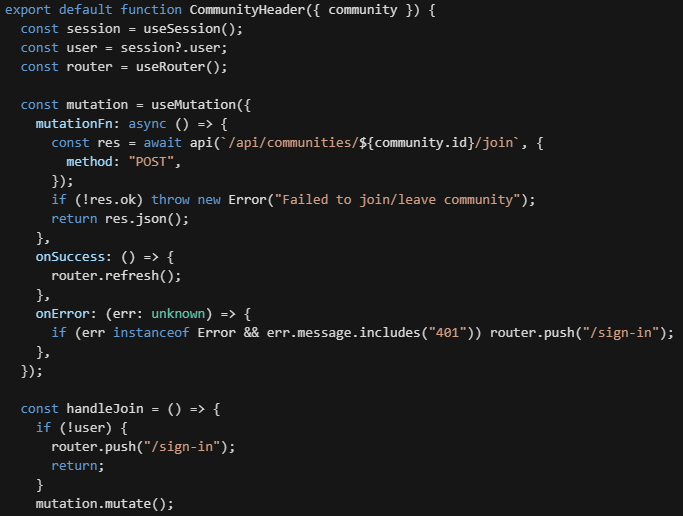
\includegraphics[width=0.92\linewidth,height=0.82\textheight,keepaspectratio]{images/image76.png}
  \caption{Code Snippet -- Join / Leave State}
  \label{fig:64}
\end{figure}
\begin{figure}[H]
  \centering
  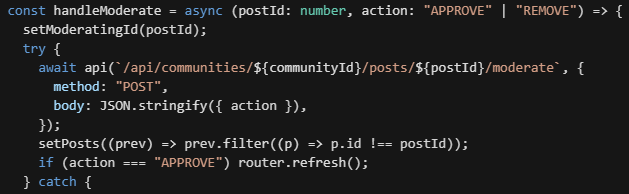
\includegraphics[width=0.92\linewidth,height=0.82\textheight,keepaspectratio]{images/image77.png}
  \caption{Code Snippet -- Moderator Pending Posts Queue}
  \label{fig:65}
\end{figure}

\subsection{Administrative Console (/admin-console)}
\begin{itemize}
  \item Server-Side Role Guarding: layout.tsx reads session details server-side. If the session is missing or the role claim is not equal to "ADMIN", the router triggers a prompt redirect (redirect("/")) before rendering any administrative markup.
  \item Global User Control (Ban/Unban): The UserTable displays a list of accounts. The administrator can click the Ban/Unban toggle, which calls the global ban endpoint. Triggering router.refresh() refreshes the table rows with the latest status.
  \item Content Report Resolution Queue (Report Queue): The ReportTable displays reported posts. It provides two operations: Dismissal (handleDismiss) which flags the report as clean and Delete Post (handleDeletePost) which removes the offending post from the system database.
\end{itemize}
\begin{figure}[H]
  \centering
  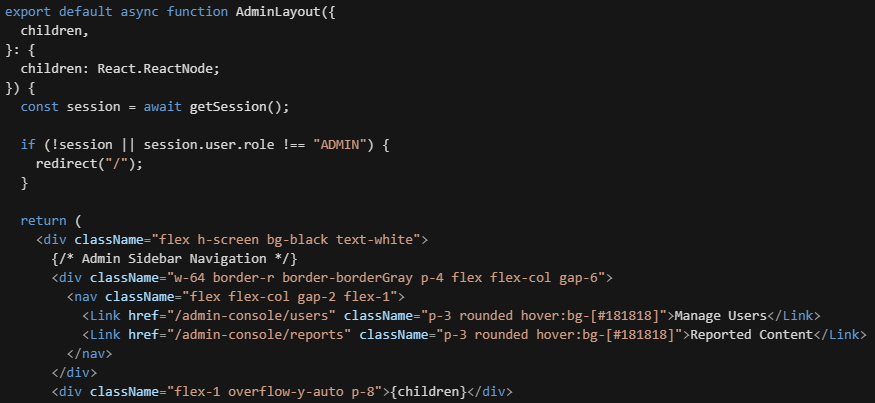
\includegraphics[width=0.92\linewidth,height=0.82\textheight,keepaspectratio]{images/image78.png}
  \caption{Code Snippet -- Administrative Layout}
  \label{fig:66}
\end{figure}
\begin{figure}[H]
  \centering
  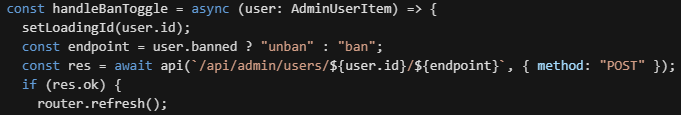
\includegraphics[width=0.92\linewidth,height=0.82\textheight,keepaspectratio]{images/image79.png}
  \caption{Code Snippet -- Banning Dashboard}
  \label{fig:67}
\end{figure}
\begin{figure}[H]
  \centering
  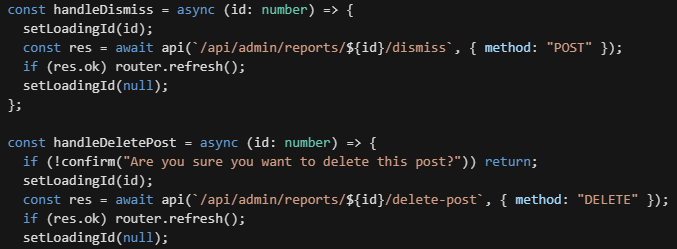
\includegraphics[width=0.92\linewidth,height=0.82\textheight,keepaspectratio]{images/image80.png}
  \caption{Code Snippet -- Report Queue}
  \label{fig:68}
\end{figure}


\chapter{TEST CASES}

\section{Detailed Cases:}
\begin{itemize}
  \item Author: Cao Ngoc Anh Tuan
  \item Date: May 30, 2026
  \item System: Breadit Social Web Platform
\end{itemize}

This document contains comprehensive test cases for the Breadit system, covering all major features and workflows based on actual system implementation.

Reference Test Accounts:
\begin{itemize}
  \item User:     user1@example.com / password
  \item Admin:    admin@breadit.dev / 123456
  \item Mod Community
\end{itemize}

\subsection{Authentication \& Account Verification}

This section demonstrates the core authentication flows. Registration and login are the entry points for all platform features. These endpoints are rate-limited (@Throttle: 10 requests per 60 seconds) and use bcrypt for secure password handling.

\subsubsection{Test Case \#: UC01}
\begin{itemize}
  \item Test Case Name: Register Account
  \item System: Breadit
  \item Subsystem: Authentication \& account verification
  \item Short Description:
  \item User registers a new account by providing a unique username, email address, and a strong password. The system validates all inputs, hashes the password with bcrypt (10 salt rounds), and dispatches a 6-digit OTP to the provided email.
  \item Pre-conditions:
  \item No existing account with the provided email or username in the database
  \item SMTP email service is configured in the backend environment
  \item The /sign-up page is accessible
\end{itemize}

\begin{longtable}{|p{0.18\linewidth}|p{0.18\linewidth}|p{0.18\linewidth}|p{0.18\linewidth}|p{0.18\linewidth}|}
\caption{UC01} \label{tab:27} \\
\hline
\textbf{Step} & \textbf{Action} & \textbf{System Response} & \textbf{Pass/Fail} & \textbf{Comments} \\
\hline
\endfirsthead
\multicolumn{5}{l}{\textit{(Continued from previous page)}} \\
\hline
\textbf{Step} & \textbf{Action} & \textbf{System Response} & \textbf{Pass/Fail} & \textbf{Comments} \\
\hline
\endhead
\hline \multicolumn{5}{r}{\textit{Continued on next page}} \\
\endfoot
\hline
\endlastfoot
01 & Submit registration form at /sign-up & Calls register API & Pass &  \\
\hline
02 & System validates inputs & Checks format and password strength & Pass &  \\
\hline
03 & System checks duplicate & Queries DB (returns 409 if duplicate) & Pass &  \\
\hline
04 & System hashes passwords and saves users with emailVerified: null & bcrypt (10 rounds); saves User record & Pass & Bcrypt 10 rounds \\
\hline
05 & System sends OTP \& redirects & Stores token, sends email, redirects & Pass & OTP valid for 15m \\
\hline
\end{longtable}

\begin{itemize}
  \item Post-condition:
  \item A new~User~record exists in the database with~emailVerified = null
  \item A VerificationToken~row is stored
  \item User's inbox contains a verification email with the 6-digit OTP
\end{itemize}

\subsubsection{Test Case \#: UC04}
\begin{itemize}
  \item Test Case Name: Log In with Email and Password
  \item System: Breadit
  \item Subsystem: Authentication \& Account Verification
  \item Short Description:
\begin{itemize}
  \item User logs into the system using a registered email and password. The system validates credentials via bcrypt comparison and issues a JWT breadit\_session httpOnly cookie on success.
\end{itemize}
  \item Pre-conditions:
\begin{itemize}
  \item A user account with the provided email exists in the database
  \item User's email is verified (emailVerified is not null)
  \item The /sign-in page is accessible
\end{itemize}
\end{itemize}

\begin{longtable}{|p{0.18\linewidth}|p{0.18\linewidth}|p{0.18\linewidth}|p{0.18\linewidth}|p{0.18\linewidth}|}
\caption{UC04} \label{tab:28} \\
\hline
\textbf{Step} & \textbf{Action} & \textbf{System Response} & \textbf{Pass/Fail} & \textbf{Comments} \\
\hline
\endfirsthead
\multicolumn{5}{l}{\textit{(Continued from previous page)}} \\
\hline
\textbf{Step} & \textbf{Action} & \textbf{System Response} & \textbf{Pass/Fail} & \textbf{Comments} \\
\hline
\endhead
\hline \multicolumn{5}{r}{\textit{Continued on next page}} \\
\endfoot
\hline
\endlastfoot
01 & Submit credentials at /sign-in & Calls login API & Pass &  \\
\hline
02 & System queries user & Finds user by email & Pass &  \\
\hline
03 & System compares password & Compares bcrypt hash & Pass &  \\
\hline
04 & System generates JWT & Creates token with claims & Pass &  \\
\hline
05 & System sets session cookie & Sets breadit\_session cookie & Pass & httpOnly cookie \\
\hline
06 & System redirects to / & Redirects to homepage / & Pass &  \\
\hline
\end{longtable}

\begin{itemize}
  \item Post-condition:
\begin{itemize}
  \item Users can access all protected routes.
  \item User is redirected to the home feed at /
\end{itemize}
\end{itemize}

\subsection{Feeds \& Discovery}

This section demonstrates how users discover content. The home feed shows posts from followed users; the explore feed surfaces trending content ranked by a time-decay engagement algorithm with author-diversity enforcement. Global search spans posts, users, hashtags, and communities.

\subsubsection{Test Case \#: UC26}
\begin{itemize}
  \item Test Case Name: View Home Feed (For You)
  \item System: Breadit
  \item Subsystem: Feeds \& Discovery
  \item Short Description:
\begin{itemize}
  \item Authenticated user views a personalized home feed containing top-level posts from themselves and followed users, ordered by most recent. Community posts and replies are excluded. Blocked users are filtered out.
\end{itemize}
  \item Pre-conditions:
\begin{itemize}
  \item User is authenticated.
  \item User follows at least one other user who has published posts.
  \item Posts exist in the system.
\end{itemize}
\end{itemize}

\begin{longtable}{|p{0.18\linewidth}|p{0.18\linewidth}|p{0.18\linewidth}|p{0.18\linewidth}|p{0.18\linewidth}|}
\caption{UC26} \label{tab:29} \\
\hline
\textbf{Step} & \textbf{Action} & \textbf{System Response} & \textbf{Pass/Fail} & \textbf{Comments} \\
\hline
\endfirsthead
\multicolumn{5}{l}{\textit{(Continued from previous page)}} \\
\hline
\textbf{Step} & \textbf{Action} & \textbf{System Response} & \textbf{Pass/Fail} & \textbf{Comments} \\
\hline
\endhead
\hline \multicolumn{5}{r}{\textit{Continued on next page}} \\
\endfoot
\hline
\endlastfoot
01 & Click "For you" or navigate to / & Calls feed API with token & Pass &  \\
\hline
02 & System validates request & Optional\allowbreak{}Jwt\allowbreak{}Auth\allowbreak{}Guard checks auth & Pass &  \\
\hline
03 & System filters posts & Queries posts from self/followees & Pass & Exclude replies \\
\hline
04 & System sorts and paginates & Orders createdAt desc (limit 3) & Pass &  \\
\hline
05 & Frontend displays feed & Renders post list with scroll pagination & Pass &  \\
\hline
\end{longtable}

\begin{itemize}
  \item Post-condition:
\begin{itemize}
  \item Users see a personalized feed sorted by most recent.
  \item Interaction state (liked, saved, reposted) is correct per post.
\end{itemize}
\end{itemize}

\subsubsection{Test Case \#: UC27}
\begin{itemize}
  \item Test Case Name: View Explore Feed (Discover)
  \item System: Breadit
  \item Subsystem: Feeds \& Discovery
  \item Short Description:
\begin{itemize}
  \item User views the explore feed, which surfaces globally trending posts ranked by a time-decay engagement score. Author-diversity is enforced.
\end{itemize}
  \item Pre-conditions:
\begin{itemize}
  \item Posts exist in the system created within the last 7 days.
  \item User may be authenticated or a guest.
\end{itemize}
\end{itemize}

\begin{longtable}{|p{0.18\linewidth}|p{0.18\linewidth}|p{0.18\linewidth}|p{0.18\linewidth}|p{0.18\linewidth}|}
\caption{UC27} \label{tab:30} \\
\hline
\textbf{Step} & \textbf{Action} & \textbf{System Response} & \textbf{Pass/Fail} & \textbf{Comments} \\
\hline
\endfirsthead
\multicolumn{5}{l}{\textit{(Continued from previous page)}} \\
\hline
\textbf{Step} & \textbf{Action} & \textbf{System Response} & \textbf{Pass/Fail} & \textbf{Comments} \\
\hline
\endhead
\hline \multicolumn{5}{r}{\textit{Continued on next page}} \\
\endfoot
\hline
\endlastfoot
01 & Click "Explore" tab & Calls explore feed API & Pass &  \\
\hline
02 & System filters posts & Gets top-level posts from last 7 days & Pass & Last 7 days posts \\
\hline
03 & System computes scores & Calculates time-decay score & Pass &  \\
\hline
04 & System applies diversity cap & Restricts to max 3 posts per author & Pass & Max 3 posts/author \\
\hline
05 & System paginates feed & Returns ranked posts with cursor & Pass &  \\
\hline
06 & Frontend displays posts & Renders explore feed; loads on scroll & Pass &  \\
\hline
\end{longtable}

\begin{itemize}
  \item Post-condition:
\begin{itemize}
  \item User sees a trending feed ranked by engagement quality.
\end{itemize}
\end{itemize}

\subsubsection{Test Case \#: UC30}
\begin{itemize}
  \item Test Case Name: Global Search
  \item System: Breadit
  \item Subsystem: Feeds \& Discovery
  \item Short Description:
\begin{itemize}
  \item User submits a search query and receives multi-type results: matching posts, users, hashtags, and communities (up to 5 each). Queries run in parallel; results are block-filtered for authenticated users.
\end{itemize}
  \item Pre-conditions:
\begin{itemize}
  \item Search query string q is non-empty (at least 1 character)
  \item Users may be authenticated or a guest.
\end{itemize}
  \item 
\end{itemize}

\begin{longtable}{|p{0.18\linewidth}|p{0.18\linewidth}|p{0.18\linewidth}|p{0.18\linewidth}|p{0.18\linewidth}|}
\caption{UC30} \label{tab:31} \\
\hline
\textbf{Step} & \textbf{Action} & \textbf{System Response} & \textbf{Pass/Fail} & \textbf{Comments} \\
\hline
\endfirsthead
\multicolumn{5}{l}{\textit{(Continued from previous page)}} \\
\hline
\textbf{Step} & \textbf{Action} & \textbf{System Response} & \textbf{Pass/Fail} & \textbf{Comments} \\
\hline
\endhead
\hline \multicolumn{5}{r}{\textit{Continued on next page}} \\
\endfoot
\hline
\endlastfoot
01 & Enter query in search bar & Calls search API & Pass &  \\
\hline
02 & System checks credentials & Optional\allowbreak{}Jwt\allowbreak{}Auth\allowbreak{}Guard runs (guests allowed) & Pass &  \\
\hline
03 & System runs searches & Runs parallel queries on posts, users, tags, communities & Pass & Parallel searches \\
\hline
04 & System groups results & Returns up to 5 items per category & Pass &  \\
\hline
05 & System paginates feed & Returns ranked posts with cursor & Pass &  \\
\hline
06 & Frontend renders results & Displays lists; navigates on click & Pass &  \\
\hline
\end{longtable}

\begin{itemize}
  \item Post-condition:
\begin{itemize}
  \item Multi-type search results displayed in sections.
  \item Clicking a result navigates to the post permalink, user profile, hashtag feed, or community page.
\end{itemize}
\end{itemize}

\subsection{Post Management}

This section covers post creation, editing, and deletion. All post mutations go through a unified multipart endpoint that handles both text content and media files. Soft delete is used to preserve referential integrity.

\subsubsection{Test Case \#: UC08}
\begin{itemize}
  \item Test Case Name: Create Text Post
  \item System: Breadit
  \item Subsystem: Post Management
  \item Short Description:
\begin{itemize}
  \item Authenticated and email-verified user creates a text post from the Share component. The system parses hashtags and @mentions, persists the post, and notifies mentioned users.
\end{itemize}
  \item Pre-conditions:
\begin{itemize}
  \item User is authenticated and email verified.
\end{itemize}
\end{itemize}

\begin{longtable}{|p{0.18\linewidth}|p{0.18\linewidth}|p{0.18\linewidth}|p{0.18\linewidth}|p{0.18\linewidth}|}
\caption{UC08} \label{tab:32} \\
\hline
\textbf{Step} & \textbf{Action} & \textbf{System Response} & \textbf{Pass/Fail} & \textbf{Comments} \\
\hline
\endfirsthead
\multicolumn{5}{l}{\textit{(Continued from previous page)}} \\
\hline
\textbf{Step} & \textbf{Action} & \textbf{System Response} & \textbf{Pass/Fail} & \textbf{Comments} \\
\hline
\endhead
\hline \multicolumn{5}{r}{\textit{Continued on next page}} \\
\endfoot
\hline
\endlastfoot
01 & Write text and click "Post" & Submits multipart request & Pass &  \\
\hline
02 & System checks text length & Validates description & Pass & Max 255 characters \\
\hline
03 & System verifies auth status & Guards check session and verification & Pass &  \\
\hline
04 & System creates Post & Saves Post record to database & Pass &  \\
\hline
05 & System parses hashtags & Creates Hashtag and PostTag rows & Pass & Index hashtags \\
\hline
06 & System parses mention & Sends Socket.IO notifications to mention users & Pass &  \\
\hline
07 & Frontend updates feed & Prepends new post to feed & Pass &  \\
\hline
\end{longtable}

\begin{itemize}
  \item Post-condition:
\begin{itemize}
  \item Post record exists in the database.
  \item \#breadit hashtag is searchable via /hashtag/breadit feed
  \item @alice (if exists) receives a real-time MENTION notification
\end{itemize}
\end{itemize}

\subsubsection{Test Case \#: UC09}
\begin{itemize}
  \item Test Case Name: Create Post with Media (Image/Video)
  \item System: Breadit
  \item Subsystem: Post Management
  \item Short Description:
\begin{itemize}
  \item User attaches image or video files to a post. The system processes each file through Cloudinary (or local sharp fallback) and creates PostMedia rows linked to the post.
\end{itemize}
  \item 
  \item Pre-conditions:
\begin{itemize}
  \item User is authenticated and email-verified
  \item File is a valid image or video format (File size $\leq$ 500 MB per file)
\end{itemize}
\end{itemize}

\begin{longtable}{|p{0.18\linewidth}|p{0.18\linewidth}|p{0.18\linewidth}|p{0.18\linewidth}|p{0.18\linewidth}|}
\caption{UC09} \label{tab:33} \\
\hline
\textbf{Step} & \textbf{Action} & \textbf{System Response} & \textbf{Pass/Fail} & \textbf{Comments} \\
\hline
\endfirsthead
\multicolumn{5}{l}{\textit{(Continued from previous page)}} \\
\hline
\textbf{Step} & \textbf{Action} & \textbf{System Response} & \textbf{Pass/Fail} & \textbf{Comments} \\
\hline
\endhead
\hline \multicolumn{5}{r}{\textit{Continued on next page}} \\
\endfoot
\hline
\endlastfoot
01 & Attach files and click "Post" & Submits multipart request & Pass & Max 10 files, $\leq$ 500MB \\
\hline
02 & System validates files & Checks file size and mime types & Pass &  \\
\hline
03 & System uploads files & Saves to Cloudinary or falls back to Sharp & Pass &  \\
\hline
04 & System creates Post & Saves Post record to database & Pass & Association rules \\
\hline
05 & System creates PostMedia & Links media URLs to Post row & Pass &  \\
\hline
06 & Frontend renders media & Displays post with media grid & Pass &  \\
\hline
\end{longtable}

\begin{itemize}
  \item Post-condition:
\begin{itemize}
  \item Post and PostMedia records exist in the database.
  \item Posts with media are visible in the feed.
\end{itemize}
  \item 
\end{itemize}

\subsection{Post Interaction}

This section covers user engagement actions: liking, commenting (replying), reposting, and bookmarking. All interaction endpoints require authentication; most also require email verification and a non-banned account status.

\subsubsection{Test Case \#: UC15}
\begin{itemize}
  \item Test Case Name: Like / Unlike Post
  \item System: Breadit
  \item Subsystem: Post Interaction
  \item Short Description:
\begin{itemize}
  \item Authenticated user toggles the like state on a post. A LIKE notification is emitted via Socket.IO to the post owner on first like. Clicking again removes the like.
\end{itemize}
  \item Pre-conditions:
\begin{itemize}
  \item User is authenticated, email-verified, and not banned.
  \item Post exists and is not deleted.
\end{itemize}
\end{itemize}

\begin{longtable}{|p{0.18\linewidth}|p{0.18\linewidth}|p{0.18\linewidth}|p{0.18\linewidth}|p{0.18\linewidth}|}
\caption{UC15} \label{tab:34} \\
\hline
\textbf{Step} & \textbf{Action} & \textbf{System Response} & \textbf{Pass/Fail} & \textbf{Comments} \\
\hline
\endfirsthead
\multicolumn{5}{l}{\textit{(Continued from previous page)}} \\
\hline
\textbf{Step} & \textbf{Action} & \textbf{System Response} & \textbf{Pass/Fail} & \textbf{Comments} \\
\hline
\endhead
\hline \multicolumn{5}{r}{\textit{Continued on next page}} \\
\endfoot
\hline
\endlastfoot
01 & Click heart icon on post & Calls like API & Pass &  \\
\hline
02 & System verifies auth & Checks auth, verification, and ban status & Pass &  \\
\hline
03 & System checks current like & Queries Like table for user/post & Pass &  \\
\hline
04 & System toggles Like row & Deletes (unlike) or inserts (like) & Pass &  \\
\hline
05 & System sends notification & Emits Socket.IO notification to owner & Pass & Notify post owner \\
\hline
06 & Frontend updates button & Toggles heart fill and counter & Pass &  \\
\hline
\end{longtable}

\begin{itemize}
  \item Post-condition:
\begin{itemize}
  \item Like rows exist in the database
  \item Post owner receives a real-time LIKE notification (if actor $\neq$ owner)
  \item Heart icon is filled; like count incremented by 1.
\end{itemize}
\end{itemize}

\subsubsection{Test Case \#: UC10}
\begin{itemize}
  \item Test Case Name: Create Reply / Comment
  \item System: Breadit
  \item Subsystem: Post Interaction
  \item Short Description:
\begin{itemize}
  \item User replies to an existing post, creating a threaded comment. The parent post owner receives a REPLY notification. Replies support text and media attachments.
\end{itemize}
  \item Pre-conditions:
\begin{itemize}
  \item Parent posts exist and is not deleted.
\end{itemize}
\end{itemize}

\begin{longtable}{|p{0.18\linewidth}|p{0.18\linewidth}|p{0.18\linewidth}|p{0.18\linewidth}|p{0.18\linewidth}|}
\caption{UC10} \label{tab:35} \\
\hline
\textbf{Step} & \textbf{Action} & \textbf{System Response} & \textbf{Pass/Fail} & \textbf{Comments} \\
\hline
\endfirsthead
\multicolumn{5}{l}{\textit{(Continued from previous page)}} \\
\hline
\textbf{Step} & \textbf{Action} & \textbf{System Response} & \textbf{Pass/Fail} & \textbf{Comments} \\
\hline
\endhead
\hline \multicolumn{5}{r}{\textit{Continued on next page}} \\
\endfoot
\hline
\endlastfoot
01 & Type reply and click "Reply" & Calls posts API with parent ID & Pass &  \\
\hline
02 & System saves reply & Creates reply post; processes media & Pass & Link parent post ID \\
\hline
03 & System sends notification & Emits Socket.IO notification to parent owner & Pass &  \\
\hline
04 & System parses mention & Dispatches notifications to mentioned users & Pass &  \\
\hline
05 & Frontend appends reply & Displays reply in comment thread & Pass &  \\
\hline
\end{longtable}

\begin{itemize}
  \item Post-condition:
\begin{itemize}
  \item Post record with parentPostId set exists in the database.
  \item Parent post owner receives a real-time REPLY notification.
  \item Reply is visible in the comment thread below the parent post.
\end{itemize}
\end{itemize}

\subsection{User Relationship Management}

This section covers the social graph features: following users to customize the home timeline and blocking users to restrict access. Both operations include real-time feedback and cache invalidation.

\subsubsection{Test Case \#: UC18}
\begin{itemize}
  \item Test Case Name: Follow / Unfollow User
  \item System: Breadit
  \item Subsystem: User Relationship Management
  \item Short Description:
\begin{itemize}
  \item User follows another user to add their posts to the home feed. The target user receives a real-time FOLLOW notification. Clicking the button again unfollows and removes the relationship.
\end{itemize}
  \item Pre-conditions:
\begin{itemize}
  \item Follower is authenticated and not banned.
  \item Follower is viewing the target user's profile page.
\end{itemize}
\end{itemize}

\begin{longtable}{|p{0.18\linewidth}|p{0.18\linewidth}|p{0.18\linewidth}|p{0.18\linewidth}|p{0.18\linewidth}|}
\caption{UC18} \label{tab:36} \\
\hline
\textbf{Step} & \textbf{Action} & \textbf{System Response} & \textbf{Pass/Fail} & \textbf{Comments} \\
\hline
\endfirsthead
\multicolumn{5}{l}{\textit{(Continued from previous page)}} \\
\hline
\textbf{Step} & \textbf{Action} & \textbf{System Response} & \textbf{Pass/Fail} & \textbf{Comments} \\
\hline
\endhead
\hline \multicolumn{5}{r}{\textit{Continued on next page}} \\
\endfoot
\hline
\endlastfoot
01 & Click "Follow" on profile & Calls follow API & Pass &  \\
\hline
02 & System verifies auth & Guards check session and ban status & Pass &  \\
\hline
03 & System checks follow & Queries Follow table & Pass &  \\
\hline
04 & System toggles Follow & Inserts follow row or delete it & Pass &  \\
\hline
05 & System sends notification & Emits Socket.IO notification to target & Pass & Real-time follow notification \\
\hline
06 & Home feed cache updates & Home feed cache updates & Pass &  \\
\hline
\end{longtable}

\begin{itemize}
  \item Post-condition:
\begin{itemize}
  \item Follow row exists in the database.
  \item Target user's posts now appear in the follower's home feed.
  \item Target user received a FOLLOW notification.
\end{itemize}
\end{itemize}

\subsubsection{Test Case \#: UC21}
\begin{itemize}
  \item Test Case Name: Block / Unblock User
  \item System: Breadit
  \item Subsystem: User Relationship Management
  \item Short Description:
\begin{itemize}
  \item User blocks another user, removing all mutual follow relationships and filtering the blocked user from all feeds, search results, and notifications. The block is bidirectional.
\end{itemize}
  \item Pre-conditions:
\begin{itemize}
  \item Acting users are authenticated and not banned.
\end{itemize}
\end{itemize}

\begin{longtable}{|p{0.18\linewidth}|p{0.18\linewidth}|p{0.18\linewidth}|p{0.18\linewidth}|p{0.18\linewidth}|}
\caption{UC21} \label{tab:37} \\
\hline
\textbf{Step} & \textbf{Action} & \textbf{System Response} & \textbf{Pass/Fail} & \textbf{Comments} \\
\hline
\endfirsthead
\multicolumn{5}{l}{\textit{(Continued from previous page)}} \\
\hline
\textbf{Step} & \textbf{Action} & \textbf{System Response} & \textbf{Pass/Fail} & \textbf{Comments} \\
\hline
\endhead
\hline \multicolumn{5}{r}{\textit{Continued on next page}} \\
\endfoot
\hline
\endlastfoot
01 & Select "Block" on profile & Calls block API & Pass &  \\
\hline
02 & System verifies auth & Guards check session and ban status & Pass &  \\
\hline
03 & System checks block & Queries Block table & Pass &  \\
\hline
04 & System toggles Block & Inserts block row or delete it & Pass &  \\
\hline
05 & System removes follows & Deletes mutual follows in both directions & Pass & Delete mutual follows \\
\hline
06 & System filters content & Bidirectionally filters posts and search & Pass & Bidirectional \\
\hline
\end{longtable}

\begin{itemize}
  \item Post-condition:
\begin{itemize}
  \item Block row exists in the database.
  \item All mutual Follow relationships are deleted.
  \item Blocked user is excluded from feeds, search, and notifications.
\end{itemize}
\end{itemize}

\subsection{Profile Management}

This section covers profile viewing and editing. Profiles are rendered via Server-Side Rendering and include block-status checks. Profile updates use a sparse PATCH operation so only provided fields are modified.

\subsubsection{Test Case \#: UC22}
\begin{itemize}
  \item Test Case Name: View User Profile
  \item System: Breadit
  \item Subsystem: Profile Management
\end{itemize}
\begin{itemize}
  \item Short Description:
\begin{itemize}
  \item User navigates to another user's profile. The system checks block status in both directions, returns the full profile with follower/following counts, interaction options.
\end{itemize}
  \item Pre-conditions:
\begin{itemize}
  \item Target users exist and are not banned.
\end{itemize}
\end{itemize}

\begin{longtable}{|p{0.18\linewidth}|p{0.18\linewidth}|p{0.18\linewidth}|p{0.18\linewidth}|p{0.18\linewidth}|}
\caption{UC22} \label{tab:38} \\
\hline
\textbf{Step} & \textbf{Action} & \textbf{System Response} & \textbf{Pass/Fail} & \textbf{Comments} \\
\hline
\endfirsthead
\multicolumn{5}{l}{\textit{(Continued from previous page)}} \\
\hline
\textbf{Step} & \textbf{Action} & \textbf{System Response} & \textbf{Pass/Fail} & \textbf{Comments} \\
\hline
\endhead
\hline \multicolumn{5}{r}{\textit{Continued on next page}} \\
\endfoot
\hline
\endlastfoot
01 & Navigate to profile /: username & Initiates profile load & Pass &  \\
\hline
02 & System fetches user profile & Calls user detail API & Pass &  \\
\hline
03 & System checks block & Queries database for mutual block & Pass &  \\
\hline
04 & System restricts view & Returns basic details only if blocked & Pass & Restrict post view \\
\hline
05 & System returns full profile & Returns profile fields, counts, and posts & Pass &  \\
\hline
06 & Frontend displays profile & Renders header, actions, and tabs & Pass &  \\
\hline
\end{longtable}

\begin{itemize}
  \item Post-condition:
\begin{itemize}
  \item Viewers can follow, block, message, or browse the target's posts via tabs.
\end{itemize}
  \item 
\end{itemize}

\subsection{Direct Messaging}

This section covers 1:1 real-time messaging. Conversations persisted in the database and delivered in real-time via Socket.IO. Unread message counts are tracked per conversation and displayed as a badge in the sidebar.

\subsubsection{Test Case \#: UC40}
\begin{itemize}
  \item Test Case Name: Start or Find a Conversation
  \item System: Breadit
  \item Subsystem: Direct Messaging
  \item Short Description:
\begin{itemize}
  \item User initiates a direct message thread with another user. If a conversation already exists between the two, the system returns it; otherwise, a new one is created.
\end{itemize}
  \item Pre-conditions:
\begin{itemize}
  \item Initiating user is authenticated and email verified.
\end{itemize}
  \item 
\end{itemize}

\begin{longtable}{|p{0.18\linewidth}|p{0.18\linewidth}|p{0.18\linewidth}|p{0.18\linewidth}|p{0.18\linewidth}|}
\caption{UC40} \label{tab:39} \\
\hline
\textbf{Step} & \textbf{Action} & \textbf{System Response} & \textbf{Pass/Fail} & \textbf{Comments} \\
\hline
\endfirsthead
\multicolumn{5}{l}{\textit{(Continued from previous page)}} \\
\hline
\textbf{Step} & \textbf{Action} & \textbf{System Response} & \textbf{Pass/Fail} & \textbf{Comments} \\
\hline
\endhead
\hline \multicolumn{5}{r}{\textit{Continued on next page}} \\
\endfoot
\hline
\endlastfoot
01 & Click Message on profile & Calls conversation API & Pass &  \\
\hline
02 & System verifies credentials & Guards check session and verification & Pass &  \\
\hline
03 & System checks user ID & Confirms user is not messaging self & Pass &  \\
\hline
04 & System searches conversation & Queries database for existing pair & Pass &  \\
\hline
05 & System returns conversation & Returns metadata if conversation exists & Pass &  \\
\hline
06 & System creates conversation & Atomically inserts conversation \& member rows & Pass &  \\
\hline
07 & Frontend redirects & Navigates to /messages/:id & Pass & Redirect to thread \\
\hline
\end{longtable}

\begin{itemize}
  \item Post-condition:
\begin{itemize}
  \item Conversation and two ConversationMember rows exist in the database.
  \item User is navigated to the message thread at /messages/: conversationId
\end{itemize}
\end{itemize}

\subsubsection{Test Case \#: UC43}
\begin{itemize}
  \item Test Case Name: Send Text Message
  \item System: Breadit
  \item Subsystem: Direct Messaging
  \item Short Description:
\begin{itemize}
  \item User sends a text message in a conversation. The message persisted and delivered to the recipient in real-time via Socket.IO. The conversation is bumped to the top of both users' lists.
\end{itemize}
  \item Pre-conditions:
\begin{itemize}
  \item User is authenticated and email verified.
  \item User is a ConversationMember of the target conversation.
\end{itemize}
\end{itemize}

\begin{longtable}{|p{0.18\linewidth}|p{0.18\linewidth}|p{0.18\linewidth}|p{0.18\linewidth}|p{0.18\linewidth}|}
\caption{UC43} \label{tab:40} \\
\hline
\textbf{Step} & \textbf{Action} & \textbf{System Response} & \textbf{Pass/Fail} & \textbf{Comments} \\
\hline
\endfirsthead
\multicolumn{5}{l}{\textit{(Continued from previous page)}} \\
\hline
\textbf{Step} & \textbf{Action} & \textbf{System Response} & \textbf{Pass/Fail} & \textbf{Comments} \\
\hline
\endhead
\hline \multicolumn{5}{r}{\textit{Continued on next page}} \\
\endfoot
\hline
\endlastfoot
01 & Type message and click Send & Inputs text (checks $\leq$ 1000 limit) & Pass &  \\
\hline
02 & Frontend appends message & Renders message instantly in chat UI & Pass &  \\
\hline
03 & System checks credentials & Guards check auth, verification, \& member role & Pass &  \\
\hline
04 & System saves message & Inserts Message row in DB & Pass &  \\
\hline
05 & System sends message & Emits newMessage Socket.IO event & Pass & Socket.IO broadcast \\
\hline
06 & System updates activity time & Refreshes Conversation.updatedAt timestamp & Pass &  \\
\hline
07 & System returns message & Returns saved row; swaps UI card & Pass &  \\
\hline
\end{longtable}

\begin{itemize}
  \item Post-condition:
\begin{itemize}
  \item Message row persisted in the database
  \item Recipient receives the message in real-time via Socket.IO.
  \item Conversation updatedAt is refreshed; conversation appears at the top of both users' lists.
\end{itemize}
\end{itemize}

\subsection{Real-time Notifications}

This section covers the notification system. Notifications for likes, replies, reposts, follows, and mentions persisted in the database and pushed in real-time via Socket.IO. Redis is used to scale broadcasting across multiple server instances.

\subsubsection{Test Case \#: UC37}
\begin{itemize}
  \item Test Case Name: View Notification List
  \item System: Breadit
  \item Subsystem: Real-time Notifications
  \item Short Description:
\begin{itemize}
  \item Authenticated user views their paginated notification history. Notifications include LIKE, REPLY, REPOST, FOLLOW, MENTION, and COMMUNITY types with read/unread visual indicators.
\end{itemize}
  \item Pre-conditions:
\begin{itemize}
  \item At least one notification exists for the user.
\end{itemize}
\end{itemize}

\begin{longtable}{|p{0.18\linewidth}|p{0.18\linewidth}|p{0.18\linewidth}|p{0.18\linewidth}|p{0.18\linewidth}|}
\caption{UC37} \label{tab:41} \\
\hline
\textbf{Step} & \textbf{Action} & \textbf{System Response} & \textbf{Pass/Fail} & \textbf{Comments} \\
\hline
\endfirsthead
\multicolumn{5}{l}{\textit{(Continued from previous page)}} \\
\hline
\textbf{Step} & \textbf{Action} & \textbf{System Response} & \textbf{Pass/Fail} & \textbf{Comments} \\
\hline
\endhead
\hline \multicolumn{5}{r}{\textit{Continued on next page}} \\
\endfoot
\hline
\endlastfoot
01 & Click notifications bell icon & Calls notifications API & Pass &  \\
\hline
02 & System validates user session & JwtAuthGuard checks credentials & Pass &  \\
\hline
03 & System queries notifications & Fetches user notifications with details & Pass &  \\
\hline
04 & System sorts and paginates & Orders by createdAt desc & Pass & Sort desc, limit 10 \\
\hline
05 & System returns lists & Returns items; frontend renders list & Pass &  \\
\hline
06 & Click notification & Calls read API; marks record; navigates & Pass &  \\
\hline
\end{longtable}

\begin{itemize}
  \item Post-condition:
\begin{itemize}
  \item Full notification history is visible to the user.
  \item Clicked notifications are marked as read (readAt set)
\end{itemize}
\end{itemize}

\subsection{Community Management}

This section covers the community lifecycle: creation, membership, and content moderation. Communities use a role hierarchy (OWNER $\rightarrow$ MOD $\rightarrow$ MEMBER). Member posts enter a moderation queue and require approval before becoming visible in the community feed.

\subsubsection{Test Case \#: UC51}
\begin{itemize}
  \item Test Case Name: Approve / Reject Community Post
  \item System: Breadit
  \item Subsystem: Community Management
  \item Short Description:
\begin{itemize}
  \item Community OWNER or MOD reviews a pending post submitted by a MEMBER. Approving publishes the post to the community feed and notifies all members. Rejecting soft deletes the post.
\end{itemize}
  \item Pre-conditions:
\begin{itemize}
  \item At least one post with isApproved = false exists in the community
  \item Acting users are authenticated and have OWNER or MOD role in the community.
\end{itemize}
  \item 
\end{itemize}

\begin{longtable}{|p{0.18\linewidth}|p{0.18\linewidth}|p{0.18\linewidth}|p{0.18\linewidth}|p{0.18\linewidth}|}
\caption{UC51} \label{tab:42} \\
\hline
\textbf{Step} & \textbf{Action} & \textbf{System Response} & \textbf{Pass/Fail} & \textbf{Comments} \\
\hline
\endfirsthead
\multicolumn{5}{l}{\textit{(Continued from previous page)}} \\
\hline
\textbf{Step} & \textbf{Action} & \textbf{System Response} & \textbf{Pass/Fail} & \textbf{Comments} \\
\hline
\endhead
\hline \multicolumn{5}{r}{\textit{Continued on next page}} \\
\endfoot
\hline
\endlastfoot
01 & Moderator clicks Approve/Reject & Calls moderate API & Pass &  \\
\hline
02 & System verifies role & Checks if role is OWNER or MOD & Pass & Verify OWNER/MOD role \\
\hline
03 & System updates post & Sets isApproved = true or soft-deletes post & Pass &  \\
\hline
04 & System sends notification & Emits COMMUNITY\_NEW\_POST event & Pass &  \\
\hline
05 & System returns state & Removes post from queue; updates feed & Pass &  \\
\hline
\end{longtable}


\subsection{Administrative Moderation}

This section covers the admin console features. Administrators have site-wide authority to manage users (ban/unban) and handle content reports. All admin routes are protected by both JwtAuthGuard and RolesGuard requiring role = ADMIN.

\subsubsection{Test Case \#: UC62}
\begin{itemize}
  \item Test Case Name: Ban / Unban User (Admin)
  \item System: Breadit
  \item Subsystem: Administrative Moderation
  \item Short Description:
\begin{itemize}
  \item Administrator bans a user from the platform. The BannedUserGuard on all write endpoints will subsequently block any write action attempted by the banned user.
\end{itemize}
  \item Pre-conditions:
\begin{itemize}
  \item Acting user has role = ADMIN
\end{itemize}
\end{itemize}

\begin{longtable}{|p{0.18\linewidth}|p{0.18\linewidth}|p{0.18\linewidth}|p{0.18\linewidth}|p{0.18\linewidth}|}
\caption{UC62} \label{tab:43} \\
\hline
\textbf{Step} & \textbf{Action} & \textbf{System Response} & \textbf{Pass/Fail} & \textbf{Comments} \\
\hline
\endfirsthead
\multicolumn{5}{l}{\textit{(Continued from previous page)}} \\
\hline
\textbf{Step} & \textbf{Action} & \textbf{System Response} & \textbf{Pass/Fail} & \textbf{Comments} \\
\hline
\endhead
\hline \multicolumn{5}{r}{\textit{Continued on next page}} \\
\endfoot
\hline
\endlastfoot
01 & Admin clicks Ban/Unban & Calls admin ban/unban API & Pass &  \\
\hline
02 & System verifies admin & Guards verify ADMIN role & Pass & Verify ADMIN role \\
\hline
03 & System updates database & Toggles User.banned status & Pass &  \\
\hline
04 & System returns success & Returns ok response; updates table & Pass &  \\
\hline
05 & System restricts user & BannedUserGuard blocks write requests & Pass & Revoke write access \\
\hline
06 & Frontend alerts user & Displays suspension banner on reload & Pass &  \\
\hline
\end{longtable}

\begin{itemize}
  \item Post-condition:
\begin{itemize}
  \item User.banned = true in the database
  \item Banned user cannot perform any write actions (posts, likes, follows, messages{\ldots}
  \item Admin can unban at any time via POST /api/admin/users/:id/unban
\end{itemize}
\end{itemize}

\subsubsection{Test Case \#: UC65}
\begin{itemize}
  \item Test Case Name: Delete Reported Post (Admin)
  \item System: Breadit
  \item Subsystem: Administrative Moderation
  \item Short Description:
\begin{itemize}
  \item Administrator reviews the reports queue and permanently softly deletes a reported post, simultaneously closing the report. Admins receive real-time REPORT notifications via Socket.IO when a new report is submitted.
\end{itemize}
  \item Pre-conditions:
\begin{itemize}
  \item At least one OPEN report exists in the queue (Report.status = "OPEN")
  \item The reported post exists and has not been deleted.
\end{itemize}
\end{itemize}

\begin{longtable}{|p{0.18\linewidth}|p{0.18\linewidth}|p{0.18\linewidth}|p{0.18\linewidth}|p{0.18\linewidth}|}
\caption{UC65} \label{tab:44} \\
\hline
\textbf{Step} & \textbf{Action} & \textbf{System Response} & \textbf{Pass/Fail} & \textbf{Comments} \\
\hline
\endfirsthead
\multicolumn{5}{l}{\textit{(Continued from previous page)}} \\
\hline
\textbf{Step} & \textbf{Action} & \textbf{System Response} & \textbf{Pass/Fail} & \textbf{Comments} \\
\hline
\endhead
\hline \multicolumn{5}{r}{\textit{Continued on next page}} \\
\endfoot
\hline
\endlastfoot
01 & Admin clicks Delete post on report & Calls delete reported post API & Pass &  \\
\hline
02 & System verifies admin role & Guards verify ADMIN role & Pass & Verify ADMIN role \\
\hline
03 & System soft-deletes post & Sets deletedAt = now() in database & Pass & Soft-delete post \\
\hline
04 & System closes report & Sets Report.status = 'CLOSED' in & Pass &  \\
\hline
05 & Frontend updates queue & Removes report card from list & Pass &  \\
\hline
\end{longtable}

\begin{itemize}
  \item Post-condition:
\begin{itemize}
  \item Reported post is soft-deleted (deletedAt set) and hidden from all feeds
  \item Report.status = "CLOSED"; report removed from the admin queue
\end{itemize}
\end{itemize}

\section{Evaluation:}

\subsection{Performance:}

\textbf{Verification method: Quantitative --- Redis INFO telemetry}

After warming the cache with 20 consecutives explore feed requests, Redis telemetry was captured:
\begin{center}
  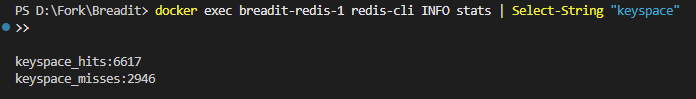
\includegraphics[width=0.92\linewidth,height=0.82\textheight,keepaspectratio]{images/image81.png}
\end{center}

Target: Cache hit rate $\geq$ 70\% under normal load (same query repeated across users)

 Redis cache reduces repeated PostgreSQL reads for trending queries.

\textbf{Verification method:~Quantitative --- k6 load test} (\texttt{docs/planning/k6\_perf\_test.js})

The explore feed endpoint (GET /api/posts?feed=explore) was tested under two scenarios:
\begin{center}
  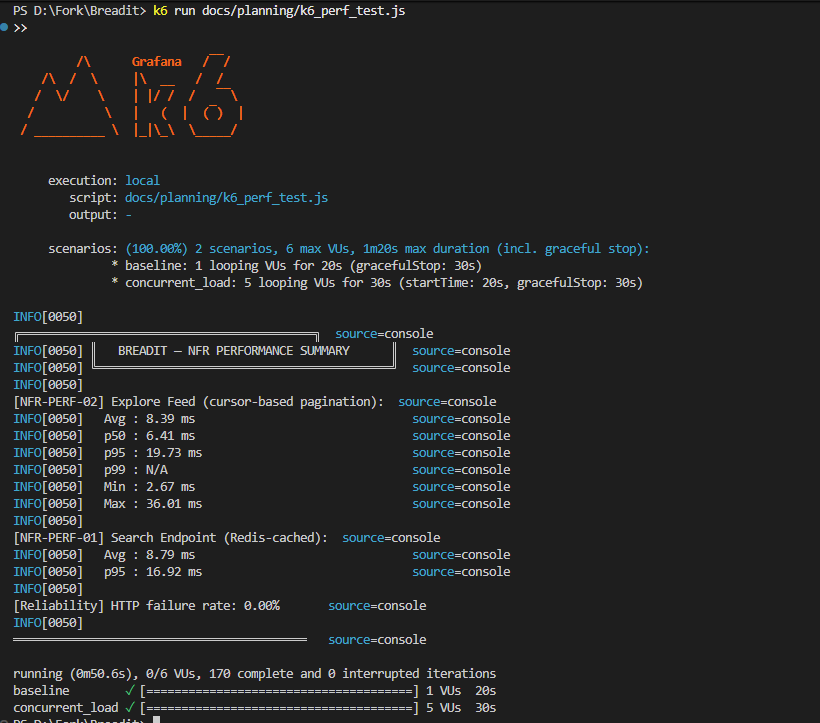
\includegraphics[width=0.92\linewidth,height=0.82\textheight,keepaspectratio]{images/image82.png}
\end{center}
\begin{itemize}
  \item Repeated requests to the same page (cursor) return cached results, observable in the significantly lower p50 vs p95 spread.
  \item Page 2 requests (new cursor) show slightly higher latency due to cache miss on first request, then drop on subsequent identical cursor requests.
\end{itemize}

\subsection{Scalability:}

\textbf{Verification method:~Qualitative + response header inspection}

The~@Throttle~decorator (10 requests per 60 seconds) is applied to authentication endpoints. Exceeding the limit returns HTTP 429 with a~Retry-After~header:
\begin{center}
  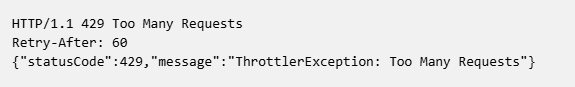
\includegraphics[width=0.92\linewidth,height=0.82\textheight,keepaspectratio]{images/image83.png}
\end{center}

\subsection{Usability:}

\textbf{Verification method:~Quantitative --- Lighthouse audit}

A Lighthouse audit was conducted on the Explore feed page ():
\begin{center}
  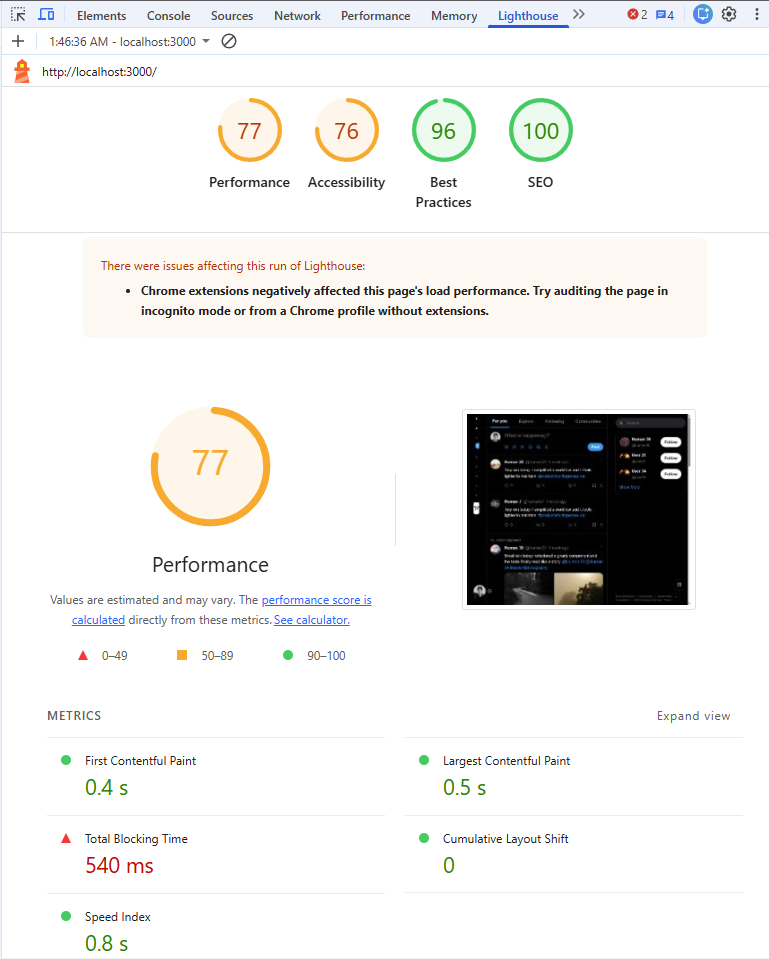
\includegraphics[width=0.92\linewidth,height=0.82\textheight,keepaspectratio]{images/image84.png}
\end{center}

\subsection{Real-Time Performance: WebSocket Notification Latency:}
\begin{center}
  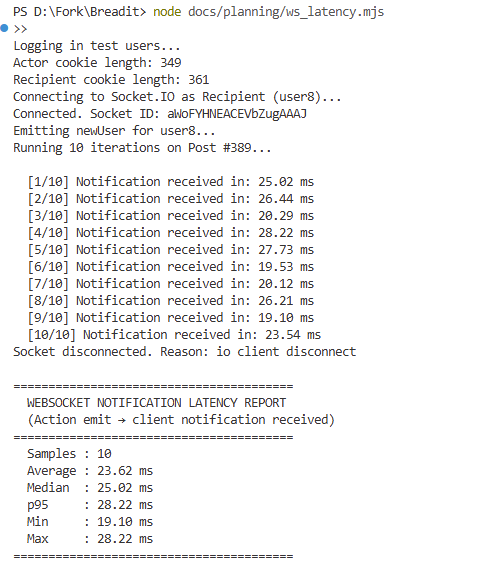
\includegraphics[width=0.92\linewidth,height=0.82\textheight,keepaspectratio]{images/image85.png}
\end{center}

\textbf{Interpretation}: The average end-to-end latency from a user action (like) to the target user's notification event arriving via Socket.IO is 23.62 ms in the local environment. This latency consists of: (1) HTTP request to NestJS $\rightarrow$ (2) database write $\rightarrow$ (3) Socket.IO emit $\rightarrow$ (4) Redis pub/sub broadcast $\rightarrow$ (5) client reception.

\subsection{Content Discovery Algorithm:}

\textbf{Qualitative Comparison: Time-Decay Scoring vs. Like-Count Baseline}

To evaluate whether the time-decay heuristic produces more relevant "trending" results than a naive like-count ranking, the following comparison was conducted using a sample of 10 posts from the local database:
\begin{center}
  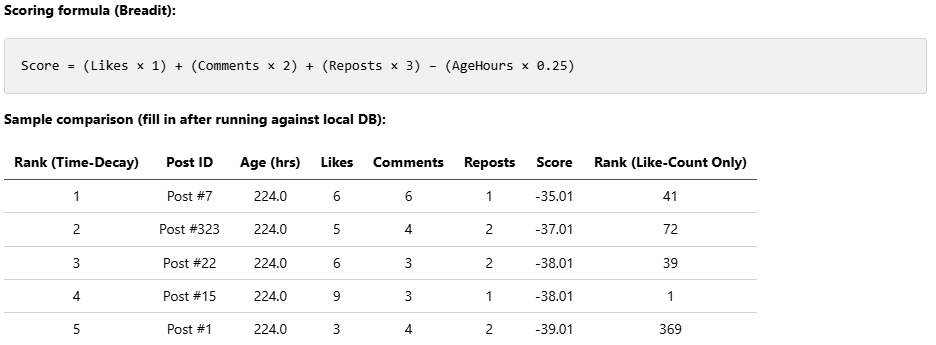
\includegraphics[width=0.92\linewidth,height=0.82\textheight,keepaspectratio]{images/image86.png}
\end{center}
\begin{itemize}
  \item Posts with high like counts but older age are ranked lower under time-decay scoring, ensuring freshness.
  \item Recent posts with moderate engagement appear higher than stale posts with higher total likes.
  \item The author-diversity filter (max 3 posts per author) prevents any single user's content from dominating the feed.
\end{itemize}

\textbf{Result:}~The time-decay heuristic demonstrably surfaces more recent, contextually relevant content compared to a naive like-count baseline, fulfilling the stated content discovery goal.


\chapter{DEMONSTRATION}

\section{User -- Features:}

\subsection{Home Page:}
\begin{figure}[H]
  \centering
  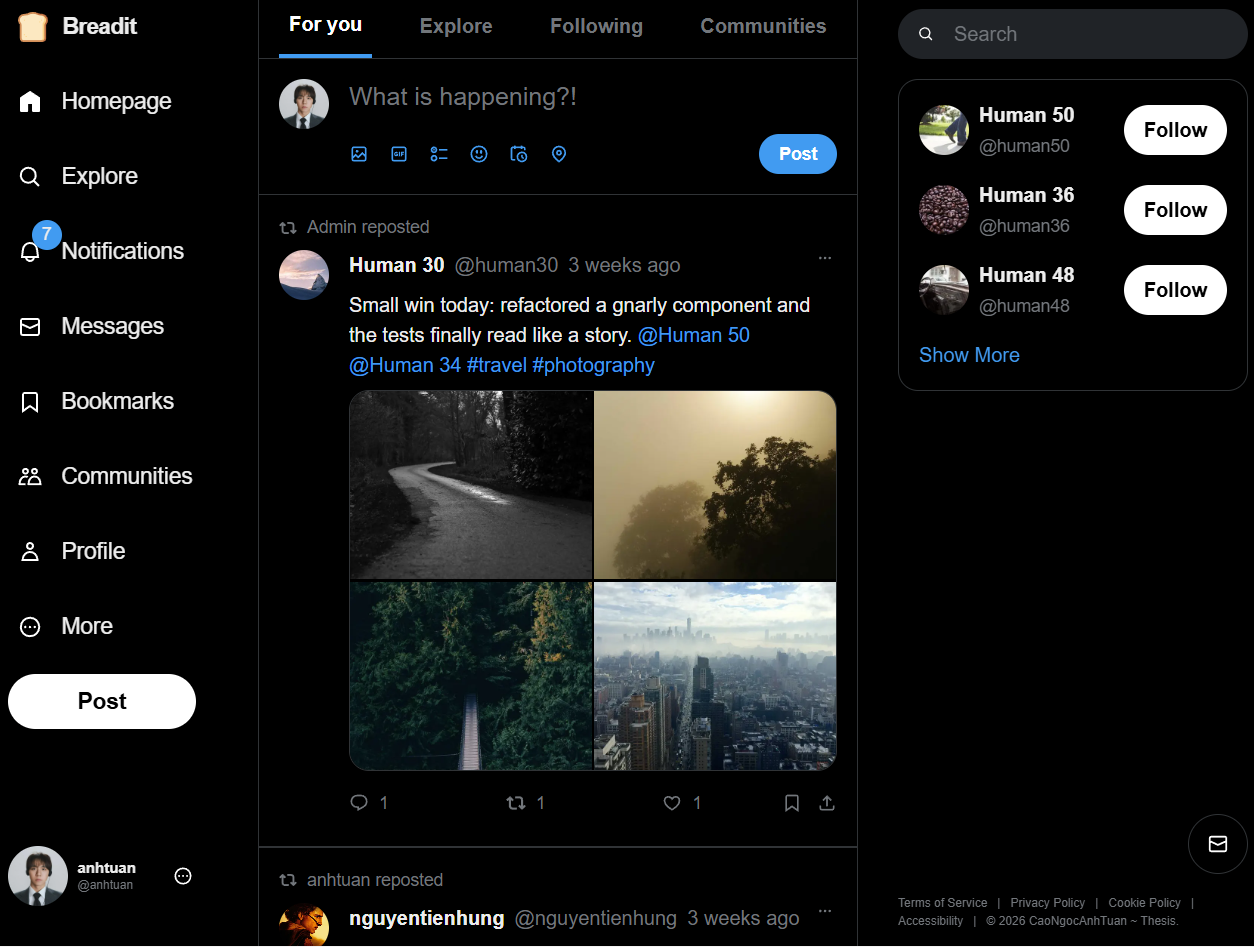
\includegraphics[width=0.92\linewidth,height=0.82\textheight,keepaspectratio]{images/image87.png}
  \caption{Home Page}
  \label{fig:69}
\end{figure}

\subsection{Sign Up Page}
\begin{figure}[H]
  \centering
  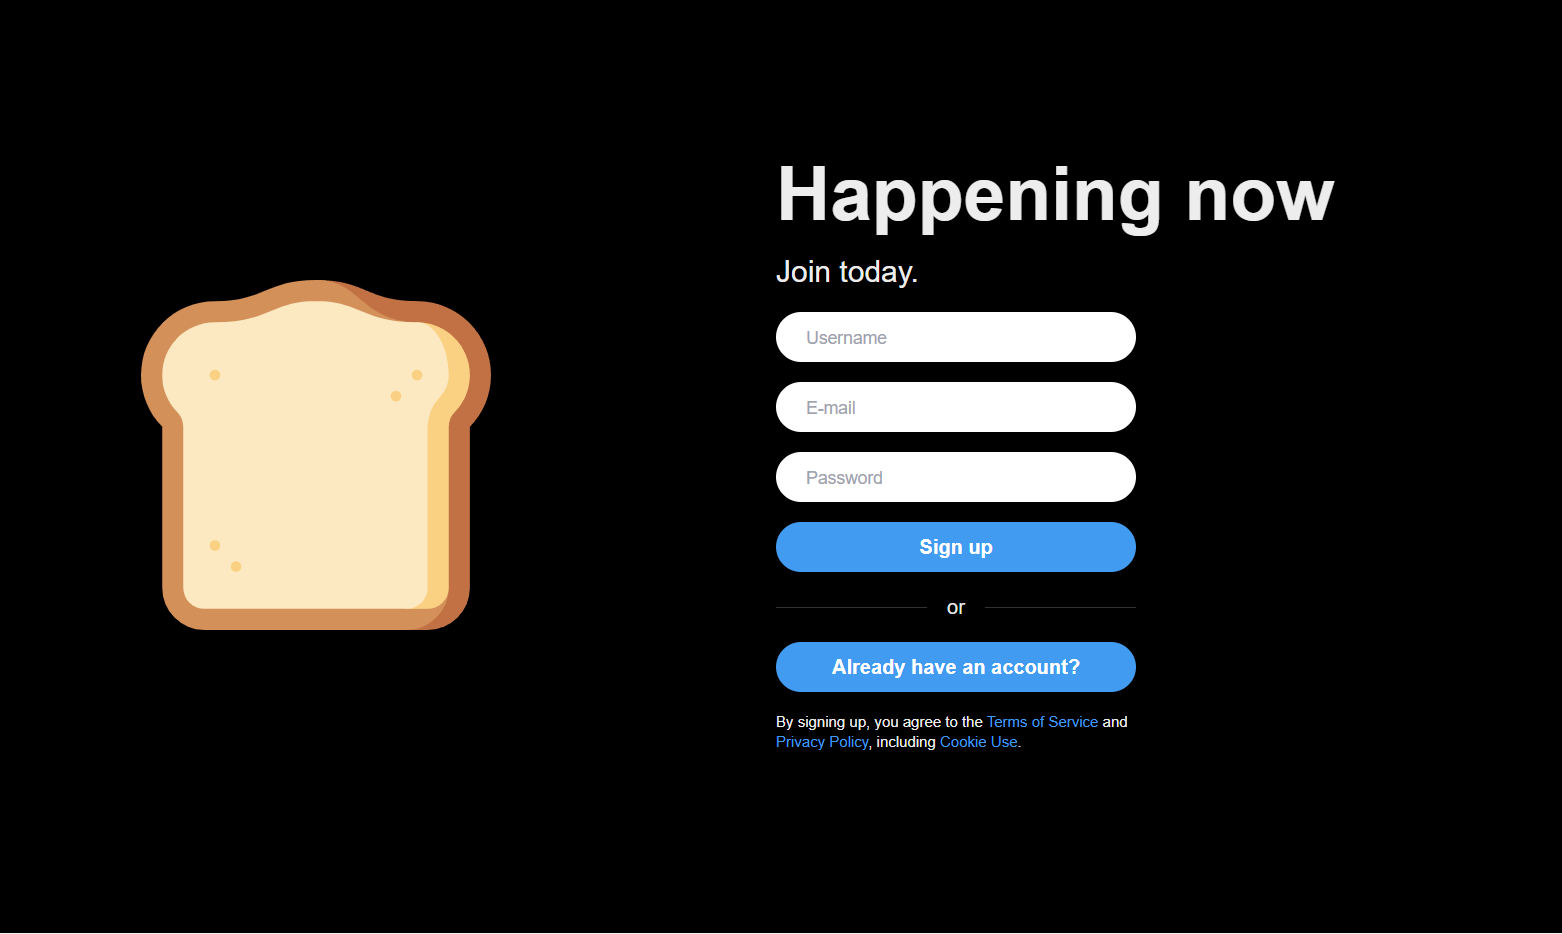
\includegraphics[width=0.92\linewidth,height=0.82\textheight,keepaspectratio]{images/image88.png}
  \caption{Sign Up Page}
  \label{fig:70}
\end{figure}

\subsection{Sign In Page}
\begin{figure}[H]
  \centering
  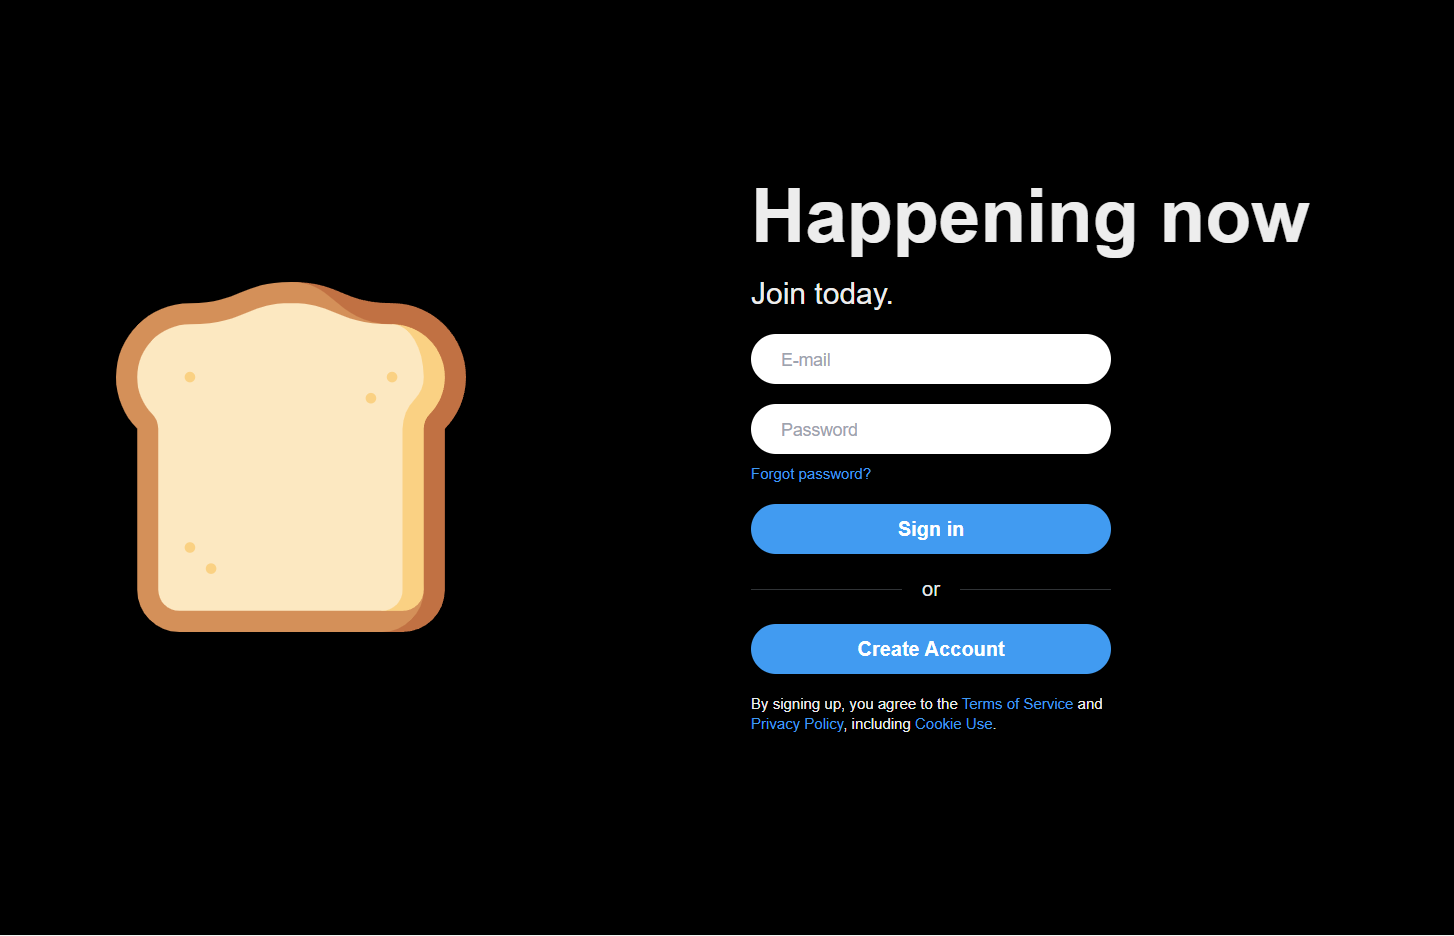
\includegraphics[width=0.92\linewidth,height=0.82\textheight,keepaspectratio]{images/image89.png}
  \caption{Sign In Page}
  \label{fig:71}
\end{figure}

\subsection{Forgot Password Page}
\begin{figure}[H]
  \centering
  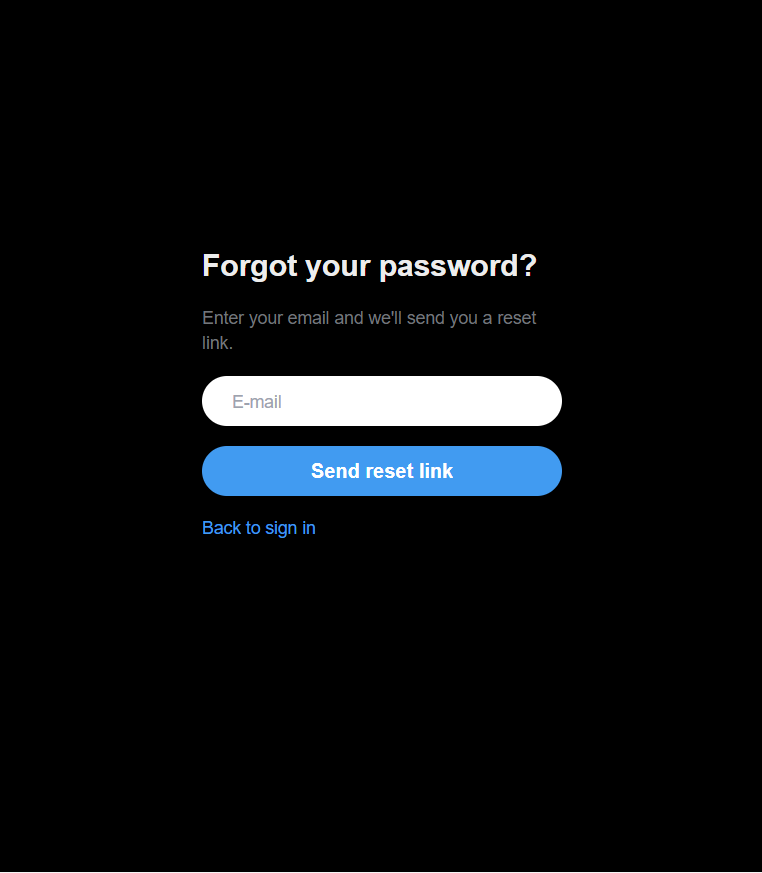
\includegraphics[width=0.92\linewidth,height=0.82\textheight,keepaspectratio]{images/image90.png}
  \caption{Forgot Password Page}
  \label{fig:72}
\end{figure}

\subsection{User Profile Page}
\begin{figure}[H]
  \centering
  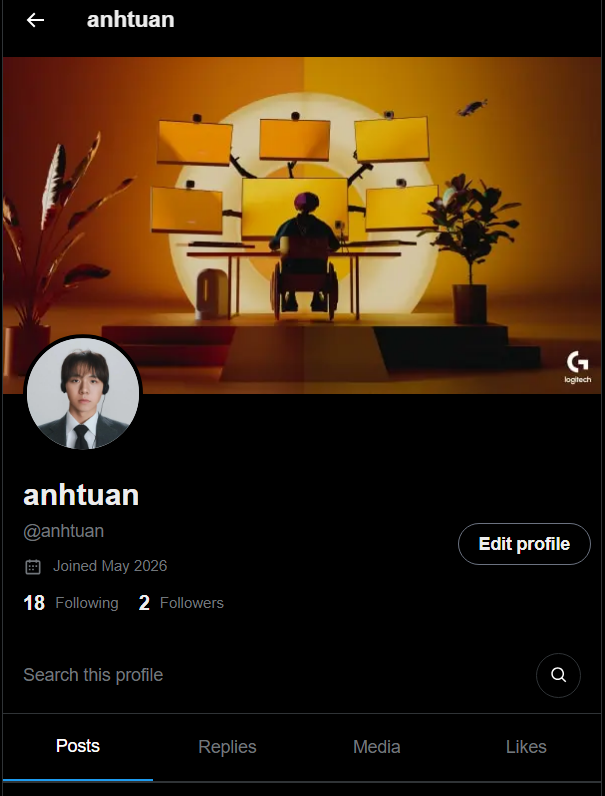
\includegraphics[width=0.92\linewidth,height=0.82\textheight,keepaspectratio]{images/image91.png}
  \caption{User Profile Page - Information Display}
  \label{fig:73}
\end{figure}

\subsection{Search Page}
\begin{figure}[H]
  \centering
  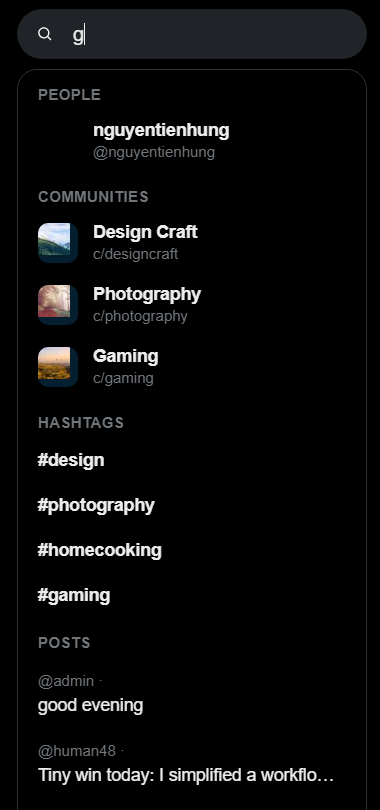
\includegraphics[width=0.92\linewidth,height=0.82\textheight,keepaspectratio]{images/image92.png}
  \caption{Search Page}
  \label{fig:74}
\end{figure}

\subsection{Message Page}
\begin{figure}[H]
  \centering
  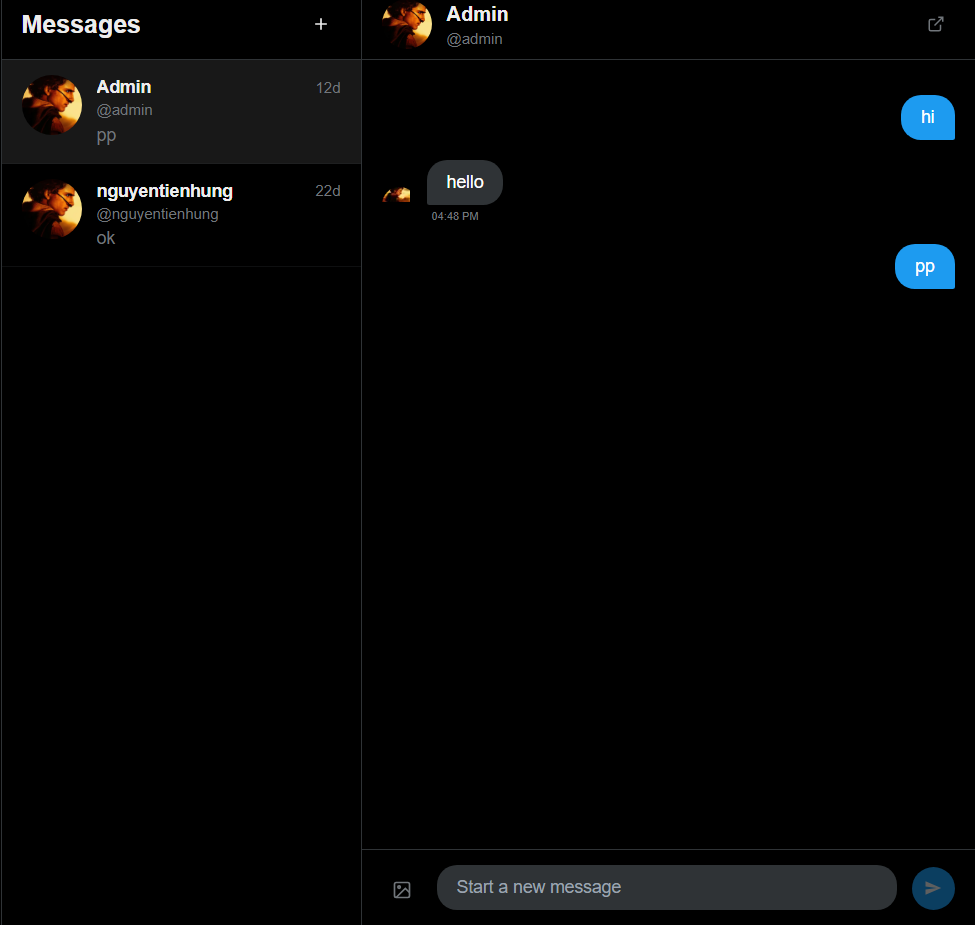
\includegraphics[width=0.92\linewidth,height=0.82\textheight,keepaspectratio]{images/image93.png}
  \caption{Message Page}
  \label{fig:75}
\end{figure}

\subsection{Bookmarks Page}
\begin{figure}[H]
  \centering
  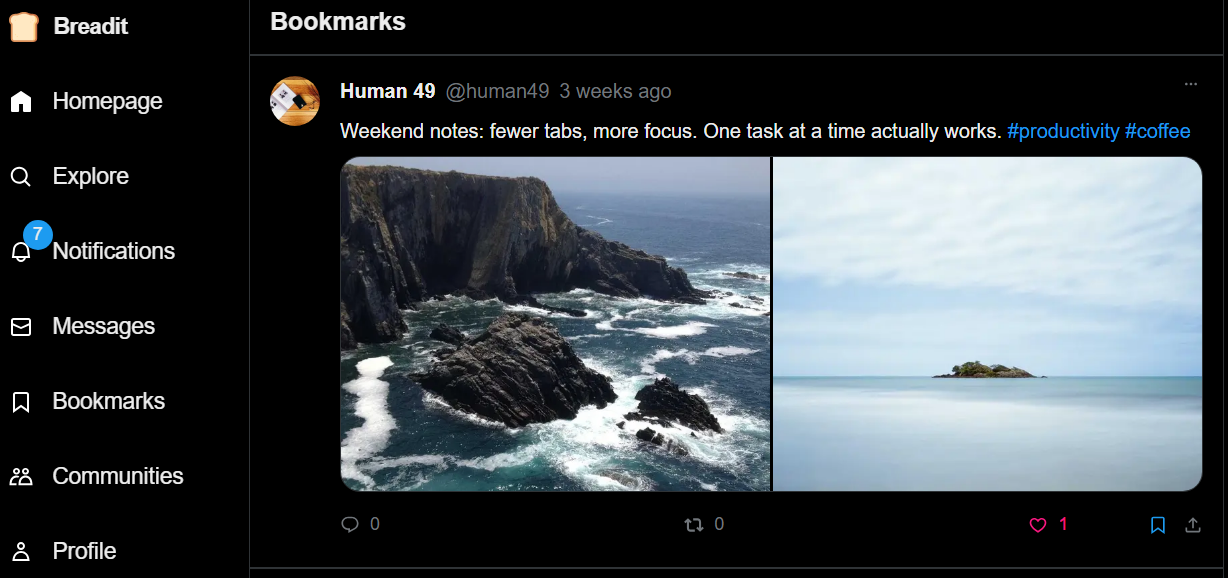
\includegraphics[width=0.92\linewidth,height=0.82\textheight,keepaspectratio]{images/image94.png}
  \caption{Bookmarks Page}
  \label{fig:76}
\end{figure}

\subsection{Notifications Page}
\begin{figure}[H]
  \centering
  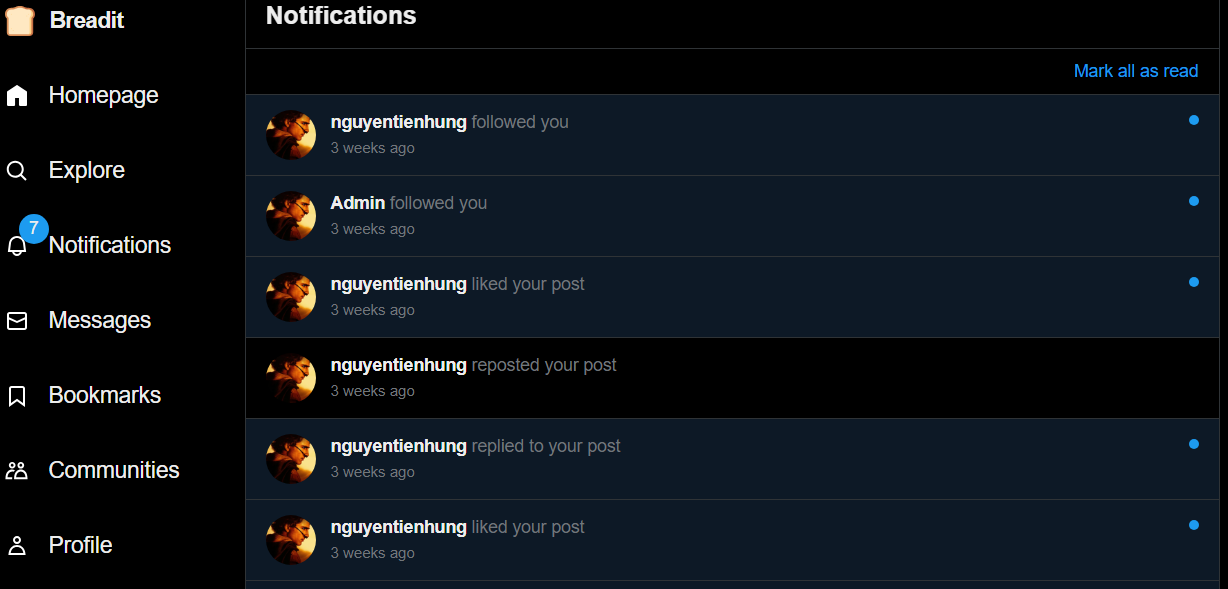
\includegraphics[width=0.92\linewidth,height=0.82\textheight,keepaspectratio]{images/image95.png}
  \caption{Notifications Page}
  \label{fig:77}
\end{figure}

\subsection{Blocked accounts Page}
\begin{figure}[H]
  \centering
  
\includegraphics[width=0.92\linewidth,height=0.82\textheight,keepaspectratio]{images/image96.png}
  \caption{Blocked accounts Page}
  \label{fig:78}
\end{figure}

\subsection{Communities Page}
\begin{figure}[H]
  \centering
  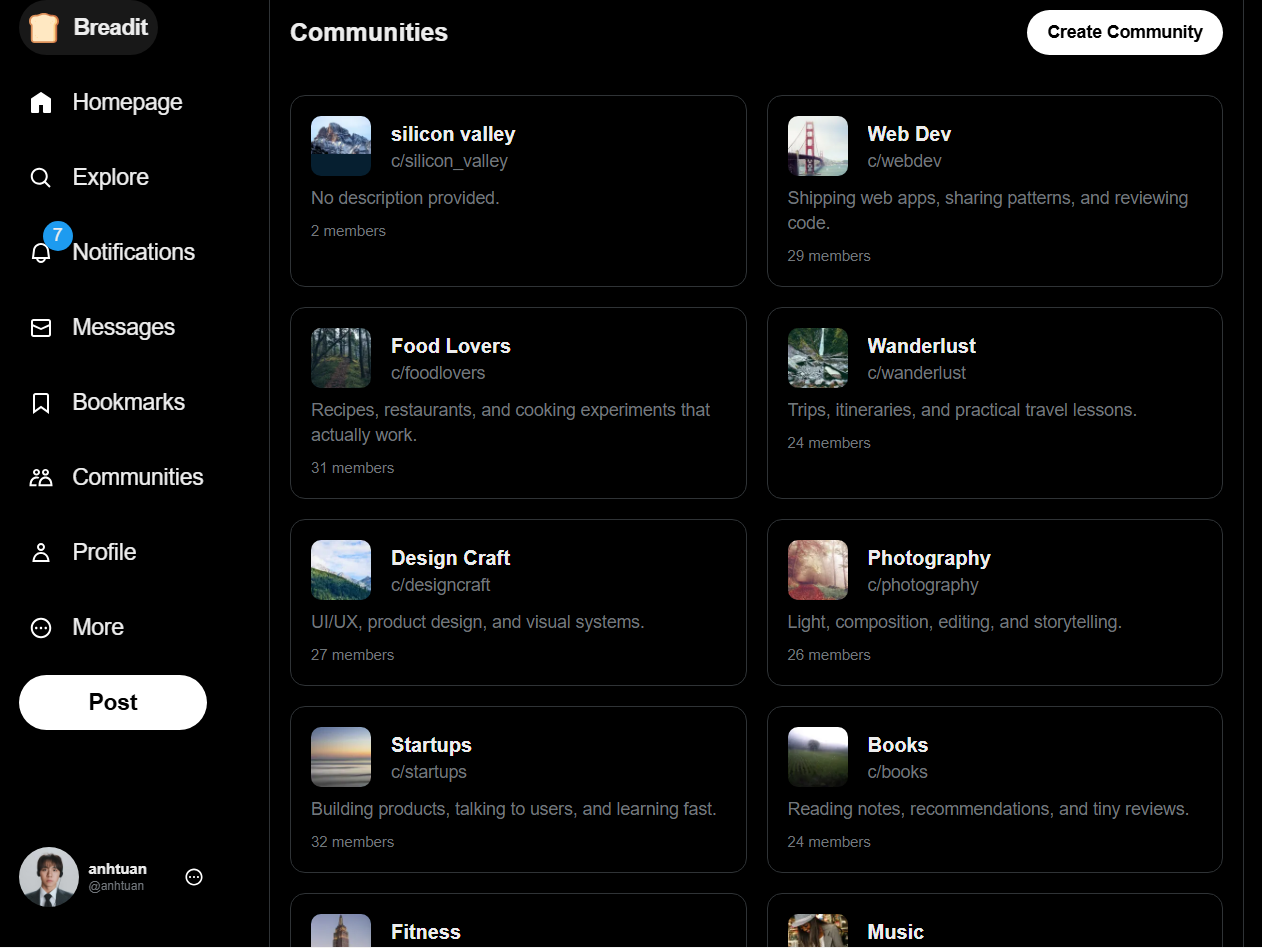
\includegraphics[width=0.92\linewidth,height=0.82\textheight,keepaspectratio]{images/image97.png}
  \caption{Communities Page}
  \label{fig:79}
\end{figure}

\subsection{Connect Page}
\begin{figure}[H]
  \centering
  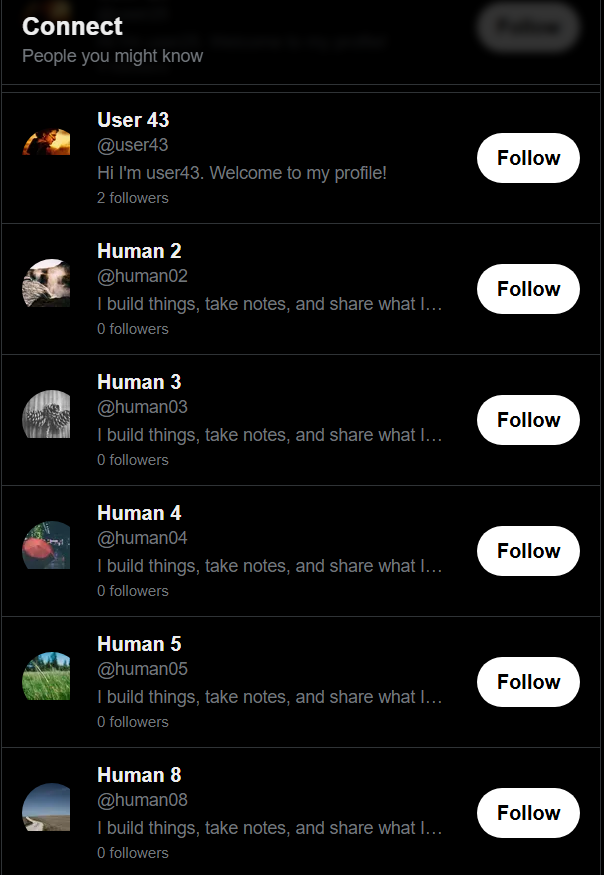
\includegraphics[width=0.92\linewidth,height=0.82\textheight,keepaspectratio]{images/image98.png}
  \caption{Connect Page}
  \label{fig:80}
\end{figure}

\subsection{Community feeds Page}
\begin{figure}[H]
  \centering
  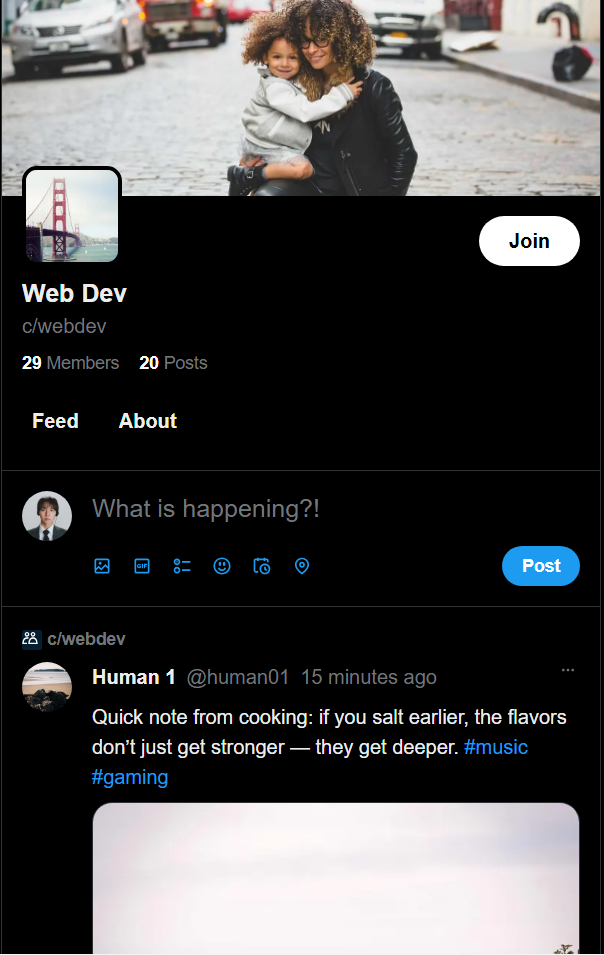
\includegraphics[width=0.92\linewidth,height=0.82\textheight,keepaspectratio]{images/image99.png}
  \caption{Community feeds Page}
  \label{fig:81}
\end{figure}

\subsection{Community rules Page}
\begin{figure}[H]
  \centering
  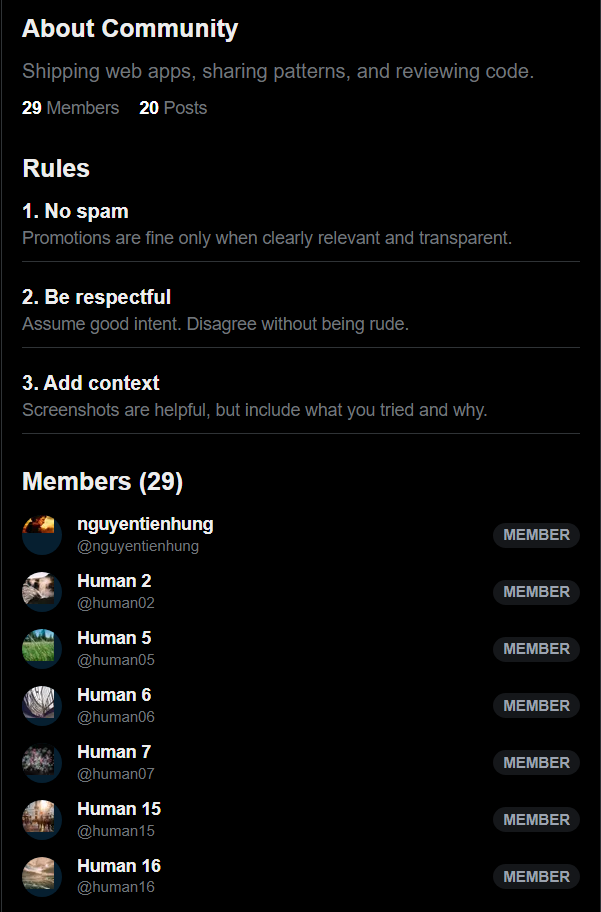
\includegraphics[width=0.92\linewidth,height=0.82\textheight,keepaspectratio]{images/image100.png}
  \caption{Community rules Page}
  \label{fig:82}
\end{figure}

\subsection{Thread comments Page}
\begin{figure}[H]
  \centering
  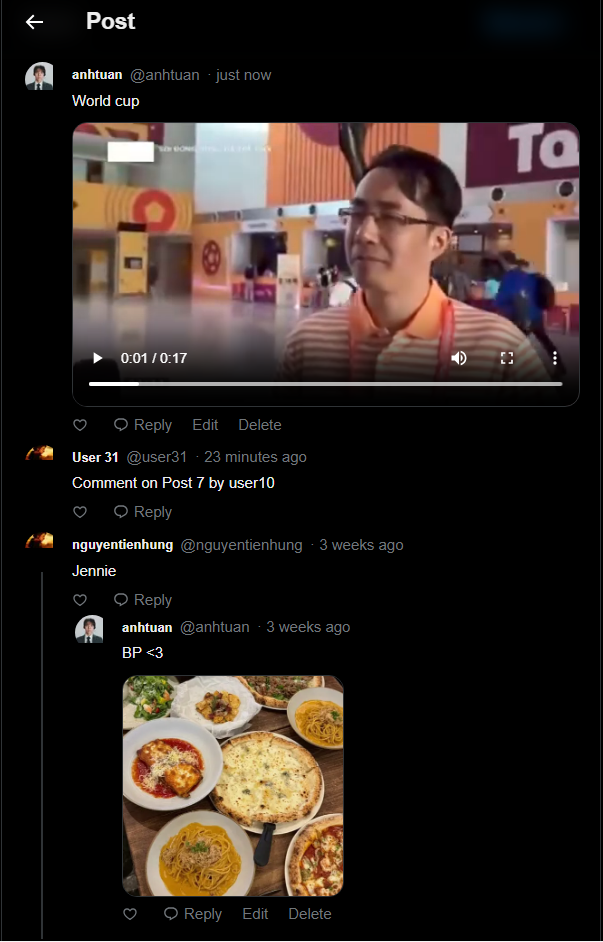
\includegraphics[width=0.92\linewidth,height=0.82\textheight,keepaspectratio]{images/image101.png}
  \caption{Thread comments Page}
  \label{fig:83}
\end{figure}

\section{Administrative Features}

\subsection{Admin Overview Page}
\begin{figure}[H]
  \centering
  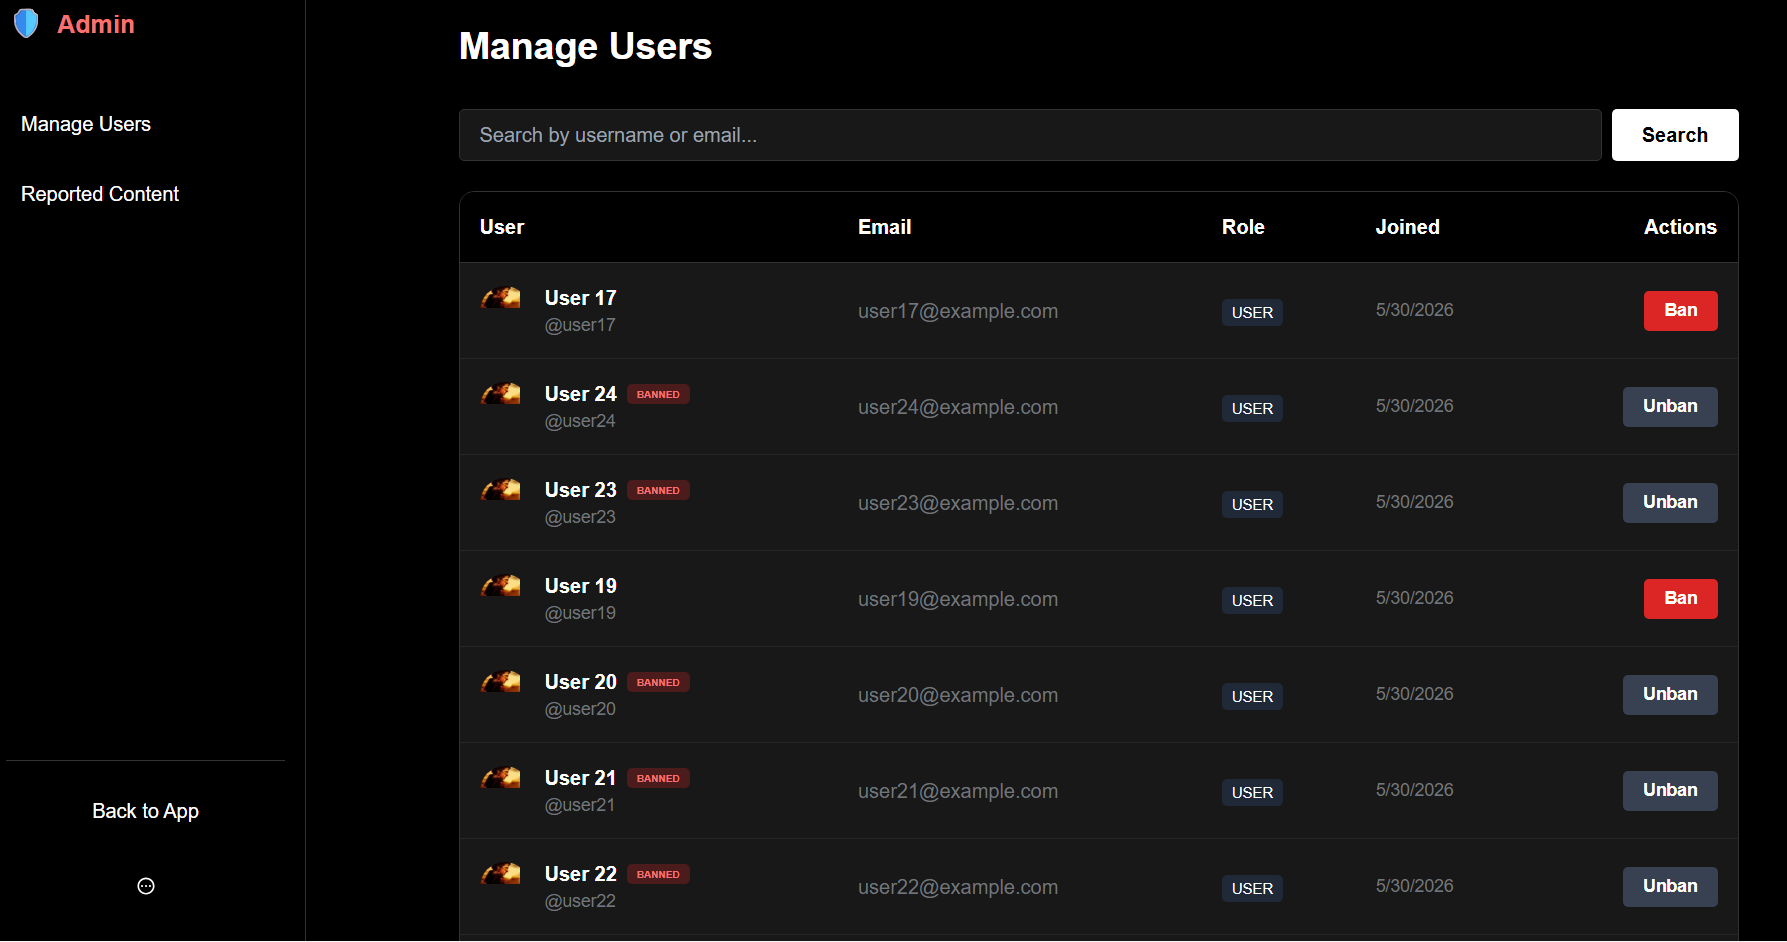
\includegraphics[width=0.92\linewidth,height=0.82\textheight,keepaspectratio]{images/image102.png}
  \caption{Admin Overview - Dashboard Access}
  \label{fig:84}
\end{figure}
\begin{figure}[H]
  \centering
  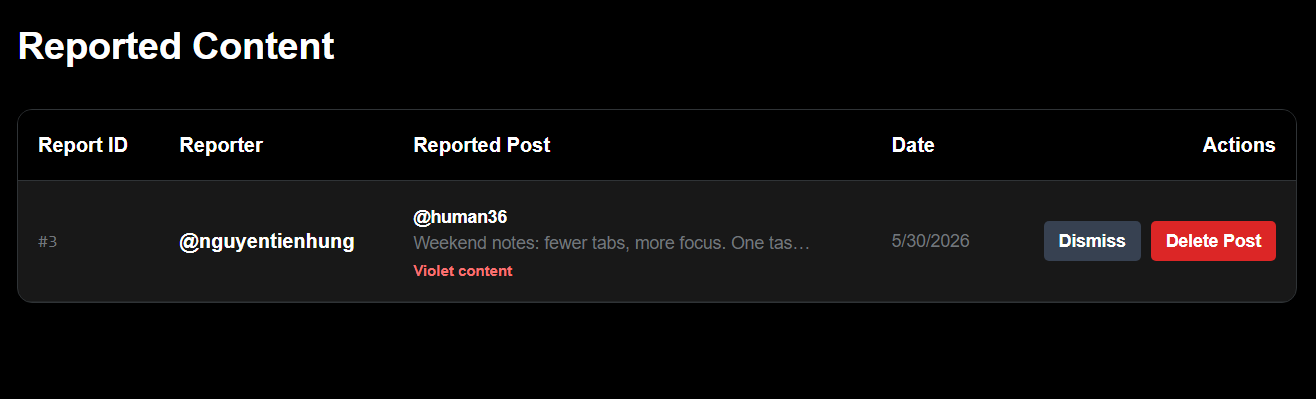
\includegraphics[width=0.92\linewidth,height=0.82\textheight,keepaspectratio]{images/image103.png}
  \caption{Admin Overview -- Report Content}
  \label{fig:85}
\end{figure}


\chapter{CONCLUSION \& FUTURE WORKS}

The Breadit Social Network Platform successfully integrates features for personalized content recommendations and real-time trending feeds, enhancing the user browsing and interaction experience. It provides a fully web-based interface accessible across modern browsers, with a responsive design that adapts to desktop and mobile viewports. The system includes both community moderator and global admin functionalities, enabling efficient content governance, user management, and report handling. Secure authentication, robust database management with PostgreSQL and Redis, and performance-optimized pagination ensure scalability and reliability, while user-friendly interfaces make the platform accessible to diverse audiences.

\section{Achievement of Research Contributions and Goals}

We evaluate the quality and success of the implemented Breadit platform against the initial Problem Statement and the three primary Research Contributions (C1, C2, C3) defined in Chapter 1:
\begin{enumerate}
  \item \textbf{C1: Hybrid Social Networking Architecture Evaluation:}
\begin{itemize}
  \item \textit{Goal:}~Address the contextual fragmentation and unorganized discussions caused by flat-reply structures in contemporary social media.
  \item \textit{Result:}~Breadit successfully unifies Reddit-style community threaded discussions and Twitter-style microblogging. Recursive parent-child relational mappings and client-side nested rendering allow multi-user conversations to maintain structural context. Qualitative validation of core use cases (UC-26, UC-27) confirmed that parallel sub-discussions co-exist without layout clutter or contextual fragmentation, satisfying Pillar 1.
\end{itemize}
\end{enumerate}
\begin{enumerate}
  \item \textbf{C2: Transparent, Deterministic Explore Feed Algorithm Evaluation:}
\begin{itemize}
  \item \textit{Goal:}~Solve the "information noise" problem and prevent content monopolization in social feeds using an auditable, deterministic ranking heuristic instead of opaque, non-interpretable machine learning models.
  \item \textit{Result:}~The content discovery engine was validated qualitatively in Section 5.5 against a like-count baseline. The empirical scoring scores proved that our linear time-decay formula () successfully penalizes older content to prioritize freshness, while the author-diversity filter (capping at 3 posts per author) ensures feed variety and prevents content monopolization, satisfying Pillar 2.
\end{itemize}
\end{enumerate}
\begin{enumerate}
  \item \textbf{C3: Real-Time Social Interaction Layer Evaluation:}
\begin{itemize}
  \item \textit{Goal:}~Deliver instant push notifications and bidirectional feedback loops without page reloads to resolve the stale user interface problems typical of traditional social networks.
  \item \textit{Result:}~The Socket.IO WebSocket gateway, integrated with a Redis Pub/Sub adapter, was validated under active load. Real-world network telemetry in Section 5.4 recorded a round-trip notification delivery latency of~\textbf{23.62 }\textbf{ms}~(from a user action like a "like" to client reception). This sub-30ms performance establishes an instant, full-duplex social interaction layer, satisfying Pillar 3.
\end{itemize}
\end{enumerate}
\begin{enumerate}
  \item \textbf{Performance, Reliability, and Security (Non-Functional Requirements):}
\begin{itemize}
  \item \textit{Goal:}~Sustain high concurrent performance, prevent database read bottlenecks, and secure sensitive authentication endpoints under load.
  \item \textit{Result:}
\begin{itemize}
  \item \textit{Caching \& Feeds:}~Redis query caching yielded a~\textbf{69.19\% hit rate}~under load. k6 load testing under concurrent load verified consistent response times for the Explore Feed (\textbf{8.39 }\textbf{ms}~average) with a~\textbf{0.00\% HTTP failure rate}, validating cursor-based pagination stability.
  \item \textit{Security:}~Custom JWT secure cookie propagation (HTTP-only) satisfies XSS mitigation (NFR-SEC-01), while Redis-backed rate limiting successfully mitigates brute-force vulnerabilities by returning HTTP 429 after 10 requests.
  \item \textit{Usability:}~Next.js SSR pre-rendering resulted in a Lighthouse~\textbf{SEO score of 100/100}~and FCP of~\textbf{400 }\textbf{ms}, ensuring indexing readiness.
\end{itemize}
\end{itemize}
\end{enumerate}

\section{System Limitations}

Despite meeting the non-functional requirements, the current Breadit implementation has several limitations that must be acknowledged:
\begin{enumerate}
  \item \textbf{Content Cold-Start Problem:}
\begin{itemize}
  \item The time-decay trending algorithm relies heavily on engagement metrics (likes, comments, reposts). Brand new posts or posts by new users with low initial visibility face a "cold-start" period where they struggle to surface in the Explore feed, even if the content is highly relevant.
\end{itemize}
  \item \textbf{Local Single-Instance Evaluation:}
\begin{itemize}
  \item Although the backend is designed to scale horizontally using a Redis Pub/Sub adapter for WebSockets and a Redis-backed throttler, the system has only been evaluated in a single-instance containerized local Docker environment. High-availability clustering, database replication lag, and multi-region network latency have not been tested under production cloud loads.
\end{itemize}
  \item \textbf{Lack of Offline Notification Fallbacks:}
\begin{itemize}
  \item Real-time notifications are only delivered if the target user is actively connected via WebSockets. The system currently lacks fallback mechanisms (such as email digests, SMS, or native Web Push notifications) to notify offline users of urgent direct messages or interactions.
\end{itemize}
  \item \textbf{Synchronous Media Processing Overhead:}
\begin{itemize}
  \item Uploading and processing images on the Fastify backend (handling multi-part files and uploading to Cloudinary) runs synchronously on the main Node.js event loop. Processing very large media payloads can block execution, temporarily slowing down concurrent lightweight API requests.
\end{itemize}
\end{enumerate}

\section{Future Works}

Provide seamless access to the Breadit Social Network across multiple platforms:

\subsection{Multi-Platform Integration}

Provide seamless access to the Breadit Social Network across multiple platforms:
\begin{itemize}
  \item \textbf{Mobile Application:}~Develop mobile apps for iOS and Android using React Native or Expo, consuming the existing NestJS REST API and Socket.IO gateway.
\begin{itemize}
  \item \textit{Full social functionality:}~Browsing feeds (For You, Explore, Hashtag, Community), creating posts with media attachments, and interacting (like, repost, comment, bookmark).
  \item \textit{Real-time push notifications:}~Push notifications for new likes, comments, mentions, follows, and direct messages.
  \item \textit{Moderation on the go:}~Community management interface for Moderators to approve posts and manage membership.
\end{itemize}
  \item \textbf{Desktop Application:}
\begin{itemize}
  \item Create a desktop version using Tauri or Electron for cross-platform compatibility (Windows, macOS, Linux).
  \item Replicate the full web feature set, optimized for larger screens and keyboard-driven navigation.
  \item Add desktop-native features such as system tray notifications for real-time events (new messages, mentions) and native file-picker integration for media uploads.
\end{itemize}
\end{itemize}

\subsection{Trending and Recommendation Module Upgrade}
\begin{itemize}
  \item \textbf{Online Scoring Pipeline:}~Upgrade the Explore Feed from its current rule-based time-decay scoring model to an online learning approach, updating post rankings in near real-time as interaction events stream in, so that trending content reflects the last few minutes of activity rather than the last cache TTL window.
  \item \textbf{Implicit Feedback Modeling:}~Extend the For You Feed offline pipeline (currently Matrix Factorization / LightFM) by incorporating richer implicit signals such as post view duration events (PostView table), allowing the model to distinguish between posts that were scrolled past and posts that were genuinely read, improving Recall@K and NDCG@K scores.
  \item \textbf{Progressive Web App (PWA) Features:}~Enable offline caching of the last-seen feed via Service Workers and a Web App Manifest, allowing users to browse cached content without an active internet connection and install Breadit as a home-screen shortcut on mobile devices.
\end{itemize}

\subsection{Enhanced AI Capabilities}
\begin{itemize}
  \item \textbf{NLP-Assisted Topic Extraction:}~Replace the current keyword-based hashtag parsing with an NLP topic extraction model that automatically infers relevant topics from post text even when the author does not include explicit hashtags, enriching feed targeting and search discovery.
  \item \textbf{Automated Toxicity Detection:}~Introduce a toxicity detection classifier (e.g., a fine-tuned BERT-based model) into the content moderation pipeline to automatically flag or quarantine posts and comments containing harmful or abusive language before they reach other users, reducing the moderation burden on Admins and Community Moderators.
  \item \textbf{Cross-Community Recommendation:}~Surface posts from communities a user have not yet joined but whose content is statistically similar to communities they actively engage with, increasing organic community discovery and platform growth.
\end{itemize}

\subsection{Public API and Integration}
\begin{itemize}
  \item \textbf{Social Login Integration:}~Integrate third-party identity providers (Google OAuth, GitHub OAuth) to enable social login, reducing registration friction and increasing conversion rates.
  \item \textbf{Public API Developer Portal:}~Expose a public API (with OAuth 2.0 scopes) allowing third-party clients to read public feeds, post on behalf of users, and embed Breadit content widgets in external websites.
  \item \textbf{Webhook Subscriptions:}~Enable webhook subscriptions so external services can receive real-time callbacks for events such as new posts in a community, enabling integration with bots, automation pipelines, and developer tooling.
\end{itemize}

\subsection{Performance Optimization}
\begin{itemize}
  \item \textbf{Database Query Performance:}~Optimize database queries for handling large post volumes efficiently, particularly the Explore feed scoring query, by introducing materialized views or pre-aggregated engagement counters that are refreshed periodically rather than computed on every request.
  \item \textbf{Cache Extension:}~Extend Redis caching beyond search results to cover user profile data, community metadata, and notification payloads, further reducing PostgreSQL read pressure during peak traffic.
  \item \textbf{Horizontally Scalable Gateway:}~Configure Socket.IO with a Redis Pub/Sub adapter to enable stateless, horizontally scaled backend deployments where WebSocket events are correctly routed across multiple server instances.
  \item \textbf{Load Testing:}~Perform regular load testing (e.g., using k6 or Artillery) to validate that the system scales gracefully under concurrent feed requests, post submissions, and WebSocket connections.
\end{itemize}

\subsection{Security Enhancements}
\begin{itemize}
  \item \textbf{Immutable Admin Audit Log:}~Implement a comprehensive Admin Audit Log---an append-only database table (AuditLog) that immutably records every administrative action (ban/unban user, delete post, dismiss report) with the acting admin's identity, target entity, reason, and timestamp, providing a non-repudiable trail for accountability.
  \item \textbf{Automated Content Filtering:}~Introduce a global word filter backed by a Redis-cached banned-word list, scanned at the backend middleware layer using the Aho-Corasick algorithm before content reaches the database, automatically flagging or blocking violating submissions in real time.
  \item \textbf{Regular Security Audits:}~Conduct regular security audits covering JWT secret rotation, httpOnly cookie configuration, CORS policy enforcement, and SQL injection surface area through Prisma's parameterized queries.
  \item \textbf{Automated End-to-End Tests:}~Implement automated end-to-end tests (e.g., using Playwright) covering authentication flows, admin moderation actions, and community permission boundaries to catch regressions in security-critical paths before deployment.
\end{itemize}


%% ── REFERENCES ───────────────────────────────────────────────────────────────
\chapter*{References}
\addcontentsline{toc}{chapter}{References}

% ── References — numbered list, matching docx format exactly ─────────────────
\begin{enumerate}[leftmargin=*, label=\arabic*., itemsep=0.8em]

  \item \textbf{Twitter Social Topology Study (Chapter 1, 2)}

  Kwak, H., Lee, C., Park, H., \& Moon, S. (2010). What is Twitter, a social network or a news media? In \textit{Proceedings of the 19th International Conference on World Wide Web} (pp.\ 591--600).

  \item \textbf{Redis Architectural Patterns (Chapter 2, 3)}

  Carlson, J. L. (2013). \textit{Redis in Action}. Manning Publications.

  \item \textbf{Algorithmic Feeds vs.\ Chronological Curation Study (Chapter 1, 2).}

  Guess, A. M., Malhotra, N., Hunt, J. B., et al. (2023). How do algorithmic feeds affect what people see, who they interact with, and what they believe? \textit{Science}, 381(6656), 398--404.

  \item \textbf{Social Content Decay Patterns (Chapter 2).}

  Lerman, K., \& Ghosh, R. (2010). Information contagion: An empirical study of the spread of news on Digg and Twitter social networks. In \textit{Proceedings of the 4th International AAAI Conference on Weblogs and Social Media} (pp.\ 90--97).

  \item \textbf{Time-Decay Feed Mechanics (Chapter 2, 3).}

  Salihefendic, A. (2015, December 8). How Hacker News ranking algorithm works. \textit{Hacking and Gonzo.} \url{https://medium.com/hacking-and-gonzo/how-hacker-news-ranking-algorithm-works-1d9b0cf2c08d}

  \item \textbf{Binomial Confidence Intervals (Wilson Score) (Chapter 2).}

  Wilson, E. B. (1927). Probable inference, the law of succession, and statistical inference. \textit{Journal of the American Statistical Association}, 22(158), 209--212.

  \item \textbf{Wilson Score Rating Application (Chapter 2).}

  Miller, E. (2009). How Not To Sort By Average Rating. \textit{Evan Miller Blog.} \url{https://www.evanmiller.org/how-not-to-sort-by-average-rating.html}

  \item \textbf{WebSocket Protocol Performance Analysis (Chapter 2).}

  Pimentel, V., \& Nickerson, B. G. (2012). Communicating and displaying real-time data with WebSocket. \textit{IEEE Internet Computing}, 16(4), 45--53.

  \item \textbf{The WebSocket Protocol Specification (Chapter 2, 3)}

  Fette, I., \& Melnikov, A. (2011). The WebSocket protocol (RFC 6455). \textit{Internet Engineering Task Force.} \url{https://www.rfc-editor.org/rfc/rfc6455}

  \item \textbf{Next.js Data Fetching \& Server Rendering Specification (Chapter 2, 3)}

  Vercel. (2026). Next.js data fetching: Server-side request routing and cookie propagation. \textit{Vercel Next.js Documentation.} \url{https://nextjs.org/docs/app/building-your-application/data-fetching}

  \item \textbf{Social Media Fatigue \& Information Overload Study (Chapter 1, 2)}

  Gupta, T., Bodhi, R., \& Pandey, A. (2024). Impact of privacy concern, information overload, and social media addiction on emotional exhaustion: an empirical study. \textit{Academy of Marketing Studies Journal}, 28(S6), 1--11.

  \item \textbf{Information Overload \& Avoidance Study (Chapter 1, 2)}

  Stamenkovi\'c, I., \& Aleksi\'c, D. (2025). Digital Overload: Fatigue and Information Avoidance on Social Media. \textit{Applied Media Studies Journal}, 6(2), 27--41.

  \item \textbf{Collaborative Filtering Foundations (Chapter 2)}

  Sarwar, B., Karypis, G., Konstan, J., \& Riedl, J. (2001). Item-based collaborative filtering recommendation algorithms. In \textit{Proceedings of the 10th International Conference on World Wide Web} (pp.\ 285--295).

  \item \textbf{NestJS Fastify Adapter Guide (Chapter 3)}

  NestJS. (2025). NestJS techniques: High-performance HTTP server integration using the Fastify adapter. \textit{NestJS Documentation.} \url{https://docs.nestjs.com/techniques/performance}

  \item \textbf{Prisma ORM Relations Guide (Chapter 3)}

  Prisma. (2026). Prisma schema relations and client integration with NestJS. \textit{Prisma ORM Documentation.} \url{https://www.prisma.io/docs/orm/prisma-schema/data-model/relations}

  \item \textbf{NestJS WebSockets Gateway Integration (Chapter 3, 5)}

  NestJS. (2025). NestJS WebSockets: Gateway decorator, connection handling, and message subscription. \textit{NestJS Documentation.} \url{https://docs.nestjs.com/websockets/gateways}

  \item \textbf{Cloudinary Upload API Reference (Chapter 3, 7)}

  Cloudinary. (2026). Cloudinary Node.js integration: Uploading files, base64 data, and buffer streams. \textit{Cloudinary Developer Documentation.} \url{https://cloudinary.com/documentation/node_integration}

  \item \textbf{Pagination API Design Patterns (Chapter 3)}

  Stripe. (2026). Pagination. \textit{Stripe API Reference.} \url{https://docs.stripe.com/api/pagination}

\end{enumerate}


%% ── APPENDIX ─────────────────────────────────────────────────────────────────
% \appendix switches counter to A, B, C... but also auto-prefixes "Appendix A"
% Using \chapter*{} suppresses that prefix so only "APPENDIX" appears
\appendix
\chapter*{APPENDIX}
\addcontentsline{toc}{chapter}{APPENDIX}
\input{chapters/appendix}

\end{document}
